% Header aus der Vorlage
\documentclass[a4paper,11pt, footheight=26pt]{scrartcl}
\usepackage[head=23pt]{geometry}	% head=23pt umgeht Fehlerwarnung, dafür größeres "top" in geometry
\geometry{a4paper, top=30mm, left=20mm, right=20mm, bottom=22mm,headsep=10mm, footskip=12mm}

% Input inkl. Umlaute, Silbentrennung
\usepackage[T1]{fontenc}
\usepackage[utf8]{inputenc}
\usepackage[ngerman]{babel}
\usepackage{csquotes}	% Anführungszeichen

% HTW Corporate Design: Arial (Helvetica)
\usepackage{helvet}
\renewcommand{\familydefault}{\sfdefault}

% Style-Aufhübschung
\usepackage{soul, color}	% Kapitälchen, Unterstrichen, Durchgestrichen usw. im Text
\usepackage{scrlayer-scrpage}	% Kopf-/Fußzeile
%\usepackage{titleref}
\usepackage[perpage]{footmisc}	% Fußnotenzählung Seitenweit, nicht Dokumentenweit

% Mathe usw.
\usepackage{amssymb}
\usepackage[fleqn]{amsmath}	% fleqn: align-Umgebung rechtsbündig
\usepackage{xcolor}
\usepackage{esint}	% Schönere Integrale, \oiint vorhanden
\everymath=\expandafter{\the\everymath\displaystyle}	% Mathe Inhalte werden weniger verkleinert
\usepackage{wasysym}	% mehr Symbole, bspw \lightning

% tikz usw.
\usepackage{tikz}
\usepackage{pgfplots}
\pgfplotsset{compat=1.11}	% Umgeht Fehlermeldung
\usetikzlibrary{graphs}
%\usetikzlibrary{through}	% ???
\usetikzlibrary{arrows}
\usetikzlibrary{arrows.meta}	% Pfeile verändern / vergrößern: \draw[-{>[scale=1.5]}] (-3,5) -> (-3,3);
\usetikzlibrary{automata,positioning} % Zeilenumbruch im Node node[align=center] {Text\\nächste Zeile}
\usetikzlibrary{patterns}	% Schraffierte Füllung
\tikzstyle{reverseclip}=[insert path={	% Inverser Clip \clip
	(current page.north east) --
	(current page.south east) --
	(current page.south west) --
	(current page.north west) --
	(current page.north east)}
% Nutzen: 
%\begin{tikzpicture}[remember picture]
%\begin{scope}
%\begin{pgfinterruptboundingbox}
%\draw [clip] DIE FLÄCHE, IN DER OBJEKT NICHT ERSCHEINEN SOLL [reverseclip];
%\end{pgfinterruptboundingbox}
%\draw DAS OBJEKT;
%\end{scope}
%\end{tikzpicture}
]	% Achtung: dafür muss doppelt kompliert werden!
\usepackage{graphpap}	% Grid für Graphen

% Tabular
\usepackage{longtable}	% Große Tabellen über mehrere Seiten
\usepackage{multirow}	% Multirow/-column: \multirow{2[Anzahl der Zeilen]}{*[Format]}{Test[Inhalt]} oder \multicolumn{7[Anzahl der Reihen]}{|c|[Format]}{Test2[Inhalt]}
\renewcommand{\arraystretch}{1.3} % Tabellenlinien nicht zu dicht
\usepackage{colortbl}
\arrayrulecolor{gray}	% heller Tabellenlinien

% Nützliches
\usepackage{verbatim}	% u.a. zum auskommentieren via \begin{comment} \end{comment}
\usepackage{tabto}	% Tabs: /tab zum nächsten Tab oder /tabto{.5 \CurrentLineWidth} zur Stelle in der Linie
\NumTabs{6}	% Anzahl von Tabs pro Zeile zum springen
\usepackage{listings} % Source-Code mit Tabs
\usepackage{lstautogobble} 
\usepackage{enumitem}	% Anpassung der enumerates
\setlist[enumerate,1]{label=\arabic*.)}	% global andere Enum-Items
\usepackage{letltxmacro} % neue Definiton von Grundbefehlen
% Nutzen:
%\LetLtxMacro{\oldemph}{\emph}
%\renewcommand{\emph}[1]{\oldemph{#1}}

% Einrichtung von lst
\lstset{
basicstyle=\ttfamily, 
mathescape=true, 
escapeinside=||, 
autogobble, 
tabsize=2,
basicstyle=\footnotesize\sffamily\color{black},
frame=single,
rulecolor=\color{lightgray},
numbers=left,
numbersep=5pt,
%basicstyle=\footnotesize\sffamily\color{black},
commentstyle=\color{gray},
%frame=single,
%numbers=left,
%numbersep=5pt,
numberstyle=\tiny\color{gray},
keywordstyle=\color{green},
%showspaces=false,
showstringspaces=false,
stringstyle=\color{orange},
tabsize=2,
literate=%
    {Ö}{{\"O}}1
    {Ä}{{\"A}}1
    {Ü}{{\"U}}1
    {ß}{{\ss}}1
    {ü}{{\"u}}1
    {ä}{{\"a}}1
    {ö}{{\"o}}1
    {~}{{\textasciitilde}}1
}

% BibTeX
\usepackage[backend=bibtex, bibencoding=ascii]{biblatex}	% BibTeX
\usepackage{makeidx}
%\makeglossary
%\makeindex

% Grafiken
\usepackage{graphicx}
\usepackage{epstopdf}	% eps-Vektorgrafiken einfügen

% pdf-Setup
\usepackage{pdfpages}
\usepackage[bookmarks,%
bookmarksopen=false,% Klappt die Bookmarks in Acrobat aus
colorlinks=true,%
linkcolor=black,%
citecolor=red,%
urlcolor=green,%
]{hyperref}

% Titel, Autor usw. werden vor dem Anfang des Dokuments in einem Rutsch definiert…
\newcommand{\DTitel}[1]{\newcommand{\Dokumententitel}{#1}}
\newcommand{\DUntertitel}[1]{\newcommand{\Dokumentenuntertitel}{#1}}
\newcommand{\DAutor}[1]{\newcommand{\Dokumentenautor}{#1}}
\newcommand{\DNotiz}[1]{\newcommand{\Dokumentennotiz}{#1}}
% … Deswegen folgendes erst Nach Dokumentenbeginn ausführen:
\AtBeginDocument{
	\hypersetup{
		pdfauthor={\Dokumentenautor},
		pdftitle={HTW Dresden | \Dokumententitel - \Dokumentenuntertitel},
	}
	\automark[section]{section}
	\automark*[subsection]{subsection}
	\pagestyle{scrheadings}
	\ihead{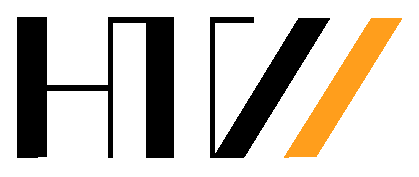
\includegraphics[height=1.7em]{../LaTeX_master/HTW-Logo.eps}}
	\ohead{\Dokumententitel}
	\ofoot{\footnotesize{\textcolor{darkgray}{Mitschrift von\\ \Dokumentenautor}}}
	% Titelseite
	\title{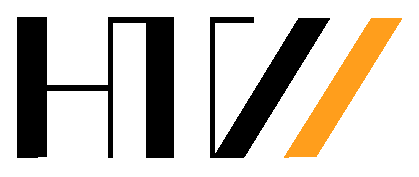
\includegraphics[width=0.35\textwidth]{../LaTeX_master/HTW-Logo.eps}\\\vspace{0.5em}
	\Huge\textbf{\Dokumententitel} \\\vspace*{0,5cm}
	\Large \Dokumentenuntertitel \\\vspace*{4cm}}
	\author{\textcolor{darkgray}{Mitschrift von \Dokumentenautor} \vspace*{1cm}\\\Dokumentennotiz}
}

%% EIGENE BEFEHLE

%Farbdefinitionen
\definecolor{red}{RGB}{180,0,0}
\definecolor{green}{RGB}{75,160,0}
\definecolor{blue}{RGB}{0,75,200}
\definecolor{orange}{RGB}{255,128,0}
\definecolor{yellow}{RGB}{255,245,0}
\definecolor{purple}{RGB}{75,0,160}
\definecolor{cyan}{RGB}{0,160,160}
\definecolor{brown}{RGB}{120,60,10}

% Textfarbe ändern
\newcommand{\tred}[1]{\textcolor{red}{#1}}
\newcommand{\tgreen}[1]{\textcolor{green}{#1}}
\newcommand{\tblue}[1]{\textcolor{blue}{#1}}
\newcommand{\torange}[1]{\textcolor{orange}{#1}}
\newcommand{\tyellow}[1]{\textcolor{yellow}{#1}}
\newcommand{\tpurple}[1]{\textcolor{purple}{#1}}
\newcommand{\tcyan}[1]{\textcolor{cyan}{#1}}
\newcommand{\tbrown}[1]{\textcolor{brown}{#1}}

% Umstellen der Tabellen Definition
\newcommand{\mpb}[1][.3]{\begin{minipage}{#1\textwidth}\vspace*{3pt}}
\newcommand{\mpe}{\vspace*{3pt}\end{minipage}}

\newcommand{\resultul}[1]{\underline{\underline{#1}}}
\newcommand{\parskp}{$ $\\}	% new line after paragraph
\newcommand{\corr}{\;\widehat{=}\;}
\newcommand{\mdeg}{^{\circ}}

\newcommand{\nok}[2]{\begin{pmatrix}#1\\#2\end{pmatrix}}	% n über k

% Definition von Titel, Autor usw.
\DTitel{Mathematik I}
\DUntertitel{Vorlesungsskript}
\DAutor{Falk-Jonatan Strube}
\DNotiz{Vorlesung von Herrn Michael Meinhold\\ \& Prof. Dr. Fabian Schwarzenberger}

\begin{document}

\maketitle
\newpage
\tableofcontents
\newpage

\chapter{Elementare Grundlagen}

\section{Aussagen und Grundzüge der Logik}
%\subsection{Aussagen, Wahrheitswert}

\paragraph{Aussage:} (im weiteren Sinne) Sprachlich sinnvoller, konsatierender Satz. In diesem Abschnitt werden nur zweiwertige Aussagen betrachtet, d.h. Aussagen, die entwoder wahr oder falsch sind.

\subparagraph{Bsp. 1:} 
\begin{itemize}
\item[(1)] Es gibt unendlich viele Primzahlen (wahr)
\item[(2)] Es gibt unendlich viele Primzahlzwillinge, z.B. (3,5), (5,7), (11,13), (17,19) usw. (Wahrheitswert nicth bekannt!)
\item[(3)] $5+7=13$ (falsch)
\item[(4)] Wie spät ist es? (keine Aussage)
\item[(5)] Diese Aussage ist falsch! (keine Aussage, paradox)
\item[(6)] Am 30.06.2016 wird es in Dresden regnen.
\end{itemize}

(1)--(3) sind zweiwertige Aussagen, (4) und (5) sind keine Aussagen, (6) ist keine zweiwertige Aussage (Wahrscheinlichkeit, d.h. Zahl zwischen 0 und 1 angebbar).

\subparagraph{Bezeichnungen:} \parskp
\begin{tabular}{l l}
p, q, r, &… Aussagen,\\
0 &… falsche Aussage, \\
1 &… wahre Aussage\\
\end{tabular}

\paragraph{Wahrheitswert:} \parskp
$w(p)=\begin{cases}
1 & \text{(falls p wahr)} \\
0 & \text{(fallls p falsch)}
\end{cases}$
    
$p \equiv q$ (p \emph{identisch} q) … p und q haben denselben Wahrheitswert
    
\subsection{Aussagesverschiebung}

\begin{enumerate}
\item \emph{Negation} $\overline{p}$ („nicht p“) [oft auch $p!$ bzw. $\neg p$]\\
\begin{tabular}{c | c}
$p$ & $\overline{p}$\\
\hline
0 & 1 \\
1 & 0 \\
\end{tabular}

\item \emph{Konjunktion} $p \wedge q$ („p und q“)
\item \emph{Disjunktion} $ p \vee q $ („p oder q“) [Alternative -- nicht ausschließendes Oder!]\\
\begin{tabular}{c | c |c |c}
$p$ & $q$ & $p \wedge q$ & $p \vee q$\\
\hline
1 & 1 &1&1\\
1 & 0 &0&1\\
0 & 1 &0&1\\
0 & 0 &0&0\\
\end{tabular}

\item \emph{Implikation} $(p \Rightarrow q ):\equiv \overline{p} \vee q$ („aus p folgt q“, „wenn p, dann q“)\\
\begin{tabular}{c | c |c|c}
$p$ & $q$ & $\overline{p}$ & $p\Rightarrow q$\\
\hline
1&1&0&1 \\
1&0&0&0\\
1&1&1&1\\
1&0&1&1\\
\end{tabular}\\
Begriffe: $p \Rightarrow q$ (p: \emph{Prämisse}, q: \emph{Konklusion})\\
Eine Implikation ist genau dann falsch, wenn die Prämisse richtig und die Konklusion falsch ist!
\paragraph{Bsp. 2:}
\begin{itemize}
\item $-1=1$ (falsch) $\Rightarrow$ $1=1$ (wahr) [durch Quadrieren]
\item $-1=1$ (falsch) $\Rightarrow$ $0=2$ (falsch) [Addition von 1]
\end{itemize}
Aus einer falschen Aussage lassen sich durch richtiges Schließen sowohl falsche als auch richtige Aussagen gewinnen.

Andere Sprechweisen: „p ist \emph{hinreichend} für q“, „q ist \emph{notwendig} für p“
\item \emph{Äquivalenz} $(p\Leftrightarrow q):\equiv (p\Rightarrow q) \wedge (q \Rightarrow p)$ („p äquivalent q“, „p ist notwendig und hinreichend für q“, „p genau dann wenn q“)\\
(ist genau dann wahr, wenn p und q den selben Wahrheitswert besitzen)
\end{enumerate}

\subsection{Logische Gesetze (Tautologien)}
Eine Tautologie $t$ ist eine Aussagenverbindung, die unabhängig vom Wahrheitswert der einzelnen Aussagen stets wahr ist (d.h. $t\equiv 1$).
\paragraph{Bsp. 3:}\parskp
Einige wichtige Tautologien
\begin{enumerate}
\item $p\Leftrightarrow \overline{\overline{p}}$ \tab \tab(Negation der Negation)
\item $p \vee \overline{p}$\tab \tab (Satz vom ausgeschlossenem Dritten)
\item a) $\overline{p\wedge q} \equiv \overline{p} \vee \overline{q}$\\
b) $\overline{p\vee q} \equiv \overline{p} \wedge \overline{q}$ \tab(de Morgansche Regeln)
\item $(p\Rightarrow q) \equiv (\overline{q} \Rightarrow \overline{p})$ \tab(Kontrapositionsgesetz)
\item $p\wedge (p\Rightarrow q)) \Rightarrow q$ \tab(direkter Beweis)
\item $p\wedge (\overline{q} \Rightarrow \overline{p})) \Rightarrow q$ \tab(indirekter Beweis)
\end{enumerate}
Beweise mittels Wahrheitstafeln (vgl. Übung 1).\\
Bemerkung zu 1., 3., 4.: Eine Äquivalenz ist genau dann eine Tautologie, wenn beide Seiten identisch sind, z.B. $p\equiv \overline{\overline{p}}$.

\paragraph{Beweistechniken:} \parskp
Zu beweisen ist $q$.
\begin{enumerate}
\item Direkter Beweis:
\begin{itemize}
\item Nachweis von $p$ (Voraussetzung)
\item Richtiger Schluss $p\Rightarrow q$\\
Dann $q$ wahr (Behauptung)
\end{itemize}
\item Indirekter Beweis: Annahme von $\overline{q}$ auf Wiederspruch führen (auf unterschiedliche Weise möglich, vgl. folgendes Bsp).
\end{enumerate}

\subparagraph{Bsp. 4:}\parskp
$q = $„$\sqrt{2}$ ist irrational“ (keine rationale Zahl)

Beweis indirekt: \\
Es gelte $\overline{q}$, d.h. $\sqrt{2}$ ist rational, dann gelten folgende Schlüsse: $\sqrt{2} = \frac{m}{n}$ mit teilerfremden natürlichen Zahlen $m$ und $n$.\\
$\Rightarrow 2=\frac{m^2}{n^2} \Rightarrow 2 \cdot n^2 = m^2 \Rightarrow 2|m^2$\\
$\Rightarrow \boxed{2|m}$ (2 ist Teiler von m)\\
$\Rightarrow 4|m^2$ (mit $m^2=2n^2$)\\
$\Rightarrow 4|2n^2 \Rightarrow 2|n^2 \Rightarrow \boxed{2|n}$\\
Widerspruch: Da $m$ und $n$ teilerfremd sind.	\#

\paragraph{Weitere Gesetze}

\begin{itemize}
\item $p\wedge q \equiv q \wedge p$\\$p\vee q \equiv q \vee p$ \tab \tab \tab(Kommutativgesetze)
\item $(p\wedge q)\wedge r \equiv p\wedge (q\wedge r)$\\$(p\vee q)\vee r \equiv p\vee (q \vee r)$ \tab \tab(Assoziativgesetze)
\item $(p\wedge q)\vee r \equiv (p \vee r) \wedge (q \vee r)$\\$(p\vee q)\wedge r \equiv (p\wedge r) \vee (q \wedge r)$ \tab(Distributivgesetze)
\item $p\wedge 1 \equiv p$, $p\vee 1 \equiv 1$, $p\wedge p \equiv p$\\$p\wedge 0 \equiv 0$, $p\vee 0 \equiv p$, $p\wedge p \equiv p$
\item $p \vee (p\wedge q ) \equiv p$ \tab \tab(Absorptionsgesetz)
\end{itemize}

\subsection{Aussagefunktionen, Quantoren, Prädikatenlogik} \label{subsec:Aussagefunktionen}
$X$ sei eine Menge (Gesamtheit von Objekten $x$ mit einem gemeinsamen Merkmal, vgl.  Abschnitt \ref{sec:Mengen})\\
$x\in X$ … $x$ ist Element von $X$. Die Objekte haben Eigenschaften (\emph{Prädikate})

\paragraph{Aussagefunktion} (auch Aussageform) $p(x)$:
Jedem $x\in X$ ist eine Aussage $p(x)$ zugeordnet. Dabei steht $x$ für ein Objekt, $p$ für ein Prädikat.
\subparagraph{Bsp. 5:}\parskp
$X$ … Menge der positiven natürlichen Zahlen (1, 2, 3, …)\\
$p(x):=$„$x$ ist eine Primzahl“\\
$p(5)$ … wahr, $p(10)$ … falsch

\paragraph{Quantoren:} \parskp
Betrachtet werden folgende Aussagen:
\begin{enumerate}
\item „Für alle $x$ (aus $X$) gilt $p(x)$“ $\equiv$ $\boxed{\forall x\; p(x)}$ (\emph{universeller Quantor} / Allquantor)
\item „Es existiert (wenigstens) ein $x$, für welches $p(x)$ gilt“ $\equiv$ $\boxed{\exists x \; p(x)}$ (\emph{existenzieller Quantor})
\end{enumerate}
Zur Schreibweise: 
\begin{itemize}
\item Bei Anwendungen (außerhalb der reinen Logik) wird oft die Grundmenke $X$ mit angegeben: \\
$\forall x \in X\; p(x)$ usw.
\item Falls sich Quantoren auf eine Teilmenge $M$ von $X$ beziehen sollen, dann können folgende Schreibweisen verwendet werden:\\
$a = \forall x \in M \; p(x)$, $b=\exists x\in M \; p(x)$.
\item Die Schreibweisen in der formalen Logik sind dann:\\
$a = \forall x \;(x \in M \Rightarrow p(x))$
\end{itemize}

\paragraph{Rechenregeln:}\parskp
$\boxed{\overline{\forall x \; p(x)} \equiv \exists x \; \overline{p(x)}}$\\
$\boxed{\overline{\exists x \; p(x)} \equiv \forall x \; \overline{p(x)}}$

\paragraph{Mehrstellige Aussagefunktionen}

\begin{itemize}
\item $p(x_1, x_2,\: ..., x_n)$,\quad $x_1 \in X_1, x_2 \in X_2,\: ... , x_n \in X_n$\\
Die Grundmengen $X_i$ können, müssen aber nicht für jede Stelle gleich sein.
\item Wird ein Quantor auf eine n-stellige Aussagefunktion angewandt, so entsteht eine (n-1)-stellige Aussagefunktion (eine 0-stellige Aussagefunktion ist eine Aussage)\\
z.B.: $\exists y \; p(x,y,z)=: q(x,z)$, die Variable $y$ wird durch den Quantor $\exists$ gebunden ($y$… gebundene Variable). Wichtig ist der Platz, nicht der Name der Variable.\\
$x, z$ … freie Variable, können durch weitere Quantoren gebunden werden.
\end{itemize}

\subparagraph{Bsp. 6:} \parskp
Ein Dorf bestehe aus 2 Teilen (Ober- und Unterdorf). Es sei $M$ die Menge aller Bewohner des Dorfes. $M_1$ bzw. $M_2$ seien die Teilmengen von $M$, die dem Ober- bzw. Unterdorf entsprechen. 

Wir betrachten folgende zweistellige Aussagefunktionen:\\
$k(x,y)$… Person $x$ (aus $M$) kennt Person $y$ (aus $M$)
\begin{enumerate} [label=\alph*)]
\item $a(x):= \forall y \; k(x,y)$… Person $x$ kennt jeden ($\Rightarrow$ „Für alle $y$ gilt: $x$ kennt $y$“)\\
$b(y):= \exists x \; k(x,y)$ … es gibt jemanden, der $y$ kennt\\
$c := \forall x \forall y \; k(x,y)$ … jeder kennt jeden\\
$d := \forall y \exists x \: k(x,y)$ … jeder wird von wenigstens einer Person gekannt\\
$e := \exists x \forall y \; k(x,y)$ … es gibt mindestens eine Person, die alle Personen kennt\\
Man beachte: \begin{itemize}
\item $d$ und $e$ sind nicht das Gleiche: Die Reihenfolge unterschiedlicher Quantoren muss beachtet werden. Bei $d$ kann für jedes $y$ ein anderes $x$ mit $k(x,y)$ existieren. Diese Abhängigkeit von $y$ wird manchmal in Anwendungen durch $\forall y \: \exists x(y) \; k(x,y)$ ausgedrückt.
\item Es gilt aber $e \Rightarrow d$ (stets wahr: Tautologie). Der Wahrheitsgehalt von z.B. $c, d, e$ kann dagegen nicht mit logischen Mitteln bestimmt werden.
\end{itemize}
\item Negation der Aussagen  bzw. Aussageformen aus a).\\
$\overline{a(x)}\equiv \exists y \; \overline{k(x,y)}$… $x$ kennt wenigstens eine Person nicht\\
$\overline{b(x)} \equiv \forall x \; \overline{k(x,y)}$ … keiner kennt $y$\\
$\overline{c} \equiv \exists x \; \overline{\forall y \; k(x,y)}\equiv \exists x \; \exists y \; \overline{k(x,y)}$ … es gibt jemanden der wenigstens eine Person nicht kennt (jemanden, der nicht alle kennt)\\
$\overline{d} \equiv \exists y \; \forall x \; \overline{k(x,y)}$… es gibt jemanden, der von keiner Person gekannt wird
$\overline{e}\equiv \forall x \; \exists y \; \overline{k(x,y)}$ … jeder kennt wenigstens eine Person nicht.
\item Folgende Aussagen sind mit Hilfe von Quantoren auszudrücken:\\
$f$… jeder aus dem Oberdorf kennt wenigstens eine Person aus dem Unterdorf.\\
$g$… es gibt jemanden im Unterdorf, der alle Personen des Oberdorfs kennt.
\begin{align*}f&=\forall x \in M_1 \; \exists y \in M_2 \; k(x,y)\\
&=\forall x \; (x \in M_1 \Rightarrow \exists y \; (y \in M_2 \wedge k(x,y)))\end{align*}
\begin{align*}
g&= \exists x \in M_2 \; \forall y \in M_1 \; k(x,y)\\
&= \exists x \; (x\in M_2 \wedge \forall y \; (y \in M_1 \Rightarrow k(x,y)))
\end{align*}
\end{enumerate}

\section{Mengen}\label{sec:Mengen}
%\subsection{Begriffe}

\paragraph{Menge:} Zusammenfassung gewisser wohl unterscheidbarer Objekte (Elemente) mit einem gemeinsamen Merkmal zu einem Ganzen.

\subparagraph{Diskussion:} Naiver Mengenbegriff führt zu Widerpsrüchen. z.B. Menge $X$ aller Mengen, die sich nicht selbst als Element enthalten.

$X=\{A | A \; Menge, A\not\in A\}$\\
$X\in X$? Wenn $X\in X \Rightarrow X\not\in X$ und $X\not\in X\Rightarrow X \in X$ (Widerspruch!).

Diese Widersprüche können umgangen werden, wenn nur Teilmengen einer sogenannten Grundmenge betrachtet werden.

\subparagraph{Bezeichungen:}
\begin{itemize}
\item meist große Buchstaben für Mengen: $A, B, ..., M, ...,X$
\item $\boxed{x\in M}$… $x$ ist Element von $M$
\item $\boxed{x\not\in M}$… $x$ ist kein Element von $M$
\end{itemize}

\subparagraph{Schreibweise:} \parskp
$M=\{\underset{\text{Elemente}}{...}\}$ oder $M = \{ x | p(x)\}$\\
mit $p(x)=$ Aussage, die genau für die Elemente $x$ aus $M$ wahr ist.

\paragraph{Wichtige Grundmengen:}
\begin{itemize}
\item $\mathbb{N}$ … Menge der natürlichen Zahlen $\{0,1,2,3,...\}$
\item $\mathbb{N}^*=\mathbb{N}\setminus \{0\} = \{1,2,3,...\}$
\item $\mathbb{Z}$ … Menge der ganzen Zahlen $\{...,-3,-2,-1,0,1,2,3,...\}$
\item $\mathbb{Q}$ … Menge der rationaln Zahlen $\{ x | x = \frac{m}{n}, m\in \mathbb{Z}, n \in \mathbb{Z}, n\not= 0\}$
\item $\mathbb{R}$ … Menge der reelen Zahlen
\item $\mathbb{C}$ … Menge der komplexen Zahlen $\{ z | z=x+ i \cdot  y,\quad x, y \in \mathbb{R}, i^2=-1\}$
\end{itemize}

\subparagraph{Bsp. 1:} \parskp
$M_1$ … Menge der Primzahlen kleiner 10, $M_1=\{2,3,5,7\}$\\
$M_2$ … Menge der reelen Zahlen zwischen 0 und 1 $M_2=\{x \in \mathbb{R}| 0<x<1\} =: \underset{\text{Intervallschreibweise}}{(0,1)}$

\paragraph{Def. 1:} (Intervallschreibweisen) \\
Es seien $a$ und $b$ reele Zahlen mit $a<b$:\\
$[a,b]:=\{ x \in \mathbb{R} | a \le x \le b\}$ … abgeschlossenes Intervall\\
$(a,b):= \{ x \in \mathbb{R} | a < x < b\}$ … offenes Intervall\\
$[a,b):= \{ x \in \mathbb{R}  | a \le x < b\}$\\
$(-\infty , a ) := \{ x \in \mathbb{R} | - \infty < x < a \} = \{x \in \mathbb{R} | x < a\}$\\
usw.

\subparagraph{Leere Menge:} z.B. $\{ x \in \mathbb{R} | x =x+1\}= \{x \in \mathbb{R} | x^2+1=0\}$ enthält kein Element.\\
Bezeichnung: $\emptyset$ oder $\{\}$

\subsection{Mengenverknüpfungen}

\paragraph{Def. 2:} \parskp
$\boxed{M_1 = M_2} : \equiv \boxed{\forall x \; (x\in M_1 \Leftrightarrow x \in M_2}$ (\emph{Gleichheit})
\paragraph{Def. 3:} \parskp
$\boxed{M_1 \subseteq M_2} : \equiv \boxed{\forall x \; (x\in M_1 \Rightarrow x \in M_2}$ (\emph{Inkulsion}) „$M_1$ ist Teilmenge von $M_2$“

\subparagraph{Diskussion:} \parskp
Ist $M_1 \subseteq M_2$ aber $M_1\not = M_2$ so kann man schreiben $M_1\subset M_2$ (echte Teilmenge).

\paragraph{Def. 4:}
\begin{enumerate}
\item \mpb 
$A\cap B := \{x | x \in A \wedge x \in B\}$\\
\emph{Durchschnitt} von $A$ und $B$
\mpe \mpb \begin{tikzpicture} [scale =0.25]
\node at (-7,3) {A};
\node at (1,3) {B};
\draw  (-5,3) ellipse (3 and 3);
\draw  (-1,3) ellipse (3 and 3);
\begin{scope} % lokal halten der Wirkung von \clip
\clip (-5,3) ellipse (3 and 3);
\draw[pattern= north east lines, pattern color=gray] (-1,3) ellipse (3 and 3);
\end{scope}
\end{tikzpicture} 
\mpe
\item \mpb
$A \cup B := \{ x | x\in A \vee x \in B\}$\\
\emph{Vereinigung} von $A$ und $B$
\mpe \mpb \begin{tikzpicture} [scale =0.25]
\draw [pattern= north east lines, pattern color=gray]  (-5,3) ellipse (3 and 3) (-1,3) ellipse (3 and 3);
\node at (-7,3) {A};
\node at (1,3) {B};
\end{tikzpicture}
\mpe
\item \mpb
$A \setminus B := \{ x | x \in A \wedge x \not\in B\}$\\
\emph{Differenz} „$A$ minus $B$“
\mpe \mpb \begin{tikzpicture} [scale =0.25, remember picture]
\draw  (-5,3) ellipse (3 and 3);
\draw  (-1,3) ellipse (3 and 3);
\begin{scope}
\begin{pgfinterruptboundingbox} % To make sure our clipping path does not mess up the placement of the picture
\draw [clip] (-5,3) ellipse (3 and 3) [reverseclip];
\end{pgfinterruptboundingbox}
\draw[pattern= north east lines, pattern color=gray] (-1,3) ellipse (3 and 3);
\end{scope}
\node at (-7,3) {A};
\node at (1,3) {B};
\end{tikzpicture} 
\mpe
\item \mpb[0.4] Bei Vorliegen einer Grundmenge $E$:\\
$\overline{A} := E \setminus A$\\
\emph{Komplimentärmenge} von $A$
\mpe \mpb \begin{tikzpicture} [scale =0.25, remember picture]
\draw  (-9,-1) rectangle (3,7);
\draw  (-5,3) ellipse (3 and 3);
\begin{scope}
\begin{pgfinterruptboundingbox} % To make sure our clipping path does not mess up the placement of the picture
\draw [clip]  (-5,3) ellipse (3 and 3) [reverseclip];
\end{pgfinterruptboundingbox}
\draw[pattern= north east lines, pattern color=gray](-9,-1) rectangle (3,7);
\end{scope}
\node at (-7,3) {A};
\node at (1,3) {E};
\end{tikzpicture}
\mpe
\end{enumerate}
\subparagraph{Diskussion:} (ausgewählte Rechenregeln)
\begin{enumerate}
\item $\cup$ und $\cap$ sind kommutativ und assoziativ\\
z.B. gilt $A \cup B = B\cup A$, $(A\cap B)\cap C = A \cap (B \cap C) = A \cap B \cap C$
\item Allg. $I$ … Indexmenge, z.B. $\{1,2,...,n\}$, $\mathbb{N}$, $\mathbb{Z}$, $\mathbb{R}$ dann:\\
$\bigcup_{i\in I}A_i := \{x| \exists i \in I \quad x \in A_i\}$\\
$\bigcap_{i\in I}A_i := \{x| \forall i \in I \quad x \in A_i\}$
\end{enumerate}

\subsection{Relationen}

\subsubsection{Grundbegriffe}

\paragraph{Def. 5:} \parskp
Die Menge $M_1 \times M_2 := \{ (x_1,x_2) | x_1 \in M_1 \wedge x_2 \in M_2\}$ heißt \emph{kartesisches Produkt} der Mengen $M_1$ und $M_2$ (= Menge aller geordneten Paare)

\subparagraph{Bsp. 2:} \parskp
$\mathbb{R}$ … Menge der reelen Zahlen, veranschaulicht durch die Zahlengerade\\
$\mathbb{R}^2 := \mathbb{R} \times \mathbb{R} = \{ (x,y) | x \in \mathbb{R} \wedge y \in \mathbb{R}\}$ … x-y-Ebene

\paragraph{Def. 6:} \parskp
Eine Teilmenge $T \subseteq M_1 \times M_2$ heißt \emph{(binäre) Relation}.

\subparagraph{Diskussion:}
\begin{enumerate}
\item Verallgemeinerung: $M_1 \times M_2 \times ... \times M_n= \{ (x_1, x_2, ..., x_n) | x_1 \in M_1, ..., x_n \in M_n\}$
(= Menge geordneter n-Tupel)\\
Eine Teilmenge $T\subseteq M_1 \times M_2 \times ... \times M_n$ heißt \emph{n-stellige Relation}.
\item \emph{Jede} Teilmenge von $M_1\times M_2$ ist eine Relation, also auch die Grenfälle $\emptyset$ (gesamt leere Menge) und $M_1\times M_2$ (vollständige Menge). Wichtig sind aber im allgemeinen die echten Teilmengen, die die verschiedensten Beziehungen zwischen den Elementen von $M_1$ und $M_2$ ausdrücken.
\end{enumerate}

\paragraph{Def. 7:}\label{Def. 7} (Eigenschaften binärer Relationen in $M_1\times M_2$)

Eine Relation $T\subseteq M_1\times M_2$ heißt:
\begin{enumerate}[label=\alph*)]
\item \emph{linksvollständig (linkstotal)}, wenn für jedes $x_1 \in M_1$ (wenigstens) ein $x_2 \in M_2$ existiert mit $(x_1, x_2) \in T$.
\item \emph{recthvollständig (rechtstotal}, wenn für jedes $x_2 \in M_2$ (wenigstens) ein $x_1 \in M_1$ existiert mit $(x_1,x_2) \in T$.
\item \emph{rechteindeutig}, wenn für jedes $x_1 \in M_1$ höchstens ein $x_2 \in M_2$ existiert mit $(x_1, x_2) \in T$.
\item \emph{linkseindeutig}, wenn für jedes $x_2 \in M_2$ höchstens ein $x_1 \in M_1$ existiert mit $(x_1, x_2) \in T$.
\end{enumerate}

\subparagraph{Bsp. 3:} \parskp
Es seien $S$ bzw. $L$ folgende Mengen von Städten bzw. Ländern:\\
$S=\{Berlin, \; Dresden, \; K\ddot{o}ln, \; Paris, \; Ram, \; Neapel, \; Oslo\}$\\
$L=\{D(eutschland), \; F(rankreich), \; B(elgien), \; I(talien), \; P(olen), \; N(orwegen)\}$\\
Die Relation $T\subseteq S \times L$ soll darstellen, welche Stadt in welchem Land liegt.\\
Man gebe $T$ elementweise an und stelle die Relation graphisch dar!\\
Welche der Eigenschaften aus Def. 7 treffen zu?
\begin{itemize}
\item $T=\{(Berlin, D), (Dresden, D), (K\ddot{o}ln, D), (Paris, F), (Rom, I), (Neapel, I), (Oslo, N)\}$
\item graphische Darstellung: \\
\begin{tikzpicture} [scale=0.25]

\draw  (0,2) rectangle (10,0) node[pos =.5]{Berlin};
\draw  (0,-1) rectangle (10,-3) node[pos =.5]{Dresden};
\draw  (0,-4) rectangle (10,-6) node[pos =.5]{Köln};
\draw  (0,-7) rectangle (10,-9) node[pos =.5]{Paris};
\draw  (0,-10) rectangle (10,-12) node[pos =.5]{Rom};
\draw  (0,-13) rectangle (10,-15) node[pos =.5]{Neapel};
\draw  (0,-16) rectangle (10,-18) node[pos =.5]{Oslo};


\draw  (18,2) rectangle (28,0) node[pos =.5]{D};
\draw  (18,-1) rectangle (28,-3) node[pos =.5]{F};
\draw  (18,-4) rectangle (28,-6) node[pos =.5]{B};
\draw  (18,-7) rectangle (28,-9) node[pos =.5]{P};
\draw  (18,-10) rectangle (28,-12) node[pos =.5]{I};
\draw  (18,-13) rectangle (28,-15) node[pos =.5]{N};

\node at (5,3) {S};
\node at (23,3) {L};
\draw[-latex] (10,1) -- (18,1);
\draw[-latex] (10,-2) -- (18,1);
\draw[-latex] (10,-5) -- (18,1);
\draw[-latex] (10,-8) -- (18,-2);
\draw[-latex] (10,-11) -- (18,-11);
\draw[-latex] (10,-14) -- (18,-11);
\draw[-latex] (10,-17) -- (18,-14);
\end{tikzpicture}\\
$(x,y) \in T: x\rightarrow y $ (gerichteter Graph)
\item Eigenschaften:\\
linksvollständig \\
nicht rechtsvollständig\\
rechtseindeutig\\
nicht linkseindeutig\\
(solche Relationen nennt man auch „Funktionen“, eindeutige Zuordnung [von Stadt $\rightarrow$ Land])
\end{itemize}

\paragraph{Def. 8:} (Eigenschaften binärer Relationen in $M\times M$)\\
Eine Relation $T\subseteq M\times M$ (Sprechweise auch „Relation auf M“) heißt…
\begin{enumerate} [label=\alph*)]
\item \emph{reflexiv}, wenn $(x,x) \in T$ für alle $x \in M$,
\item \emph{symmetrisch}, wenn $(x,y) \in T \Rightarrow (y,x) \in T$,
\item \emph{antisymmetrisch}, wenn $((x,y) \in T \wedge (y,x) \in T) \Rightarrow x=y$,
\item \emph{asymmetrisch}, wenn $(x,y) \in T \Rightarrow (y,x) \not\in T$, 
\item \emph{transitiv}, wenn $((x,y) \in T \wedge (y,z) \in T) \Rightarrow (x,z) \in T$
\end{enumerate}
… jeweils für \emph{alle} $x,y,z \in M$ gilt.

\subparagraph{Bsp. 4:} \parskp
Welche Eigenschaften aus Def. 8 besitzen folgende Relationen?\\
Es sei $P$ eine Menge von Personen.
\begin{enumerate} [label=\alph*)]
\item Eine Person $x\in P$ sei jünger als $y\in P$, wenn ihr Geburtstag später als der von $y$ ist.\\
$\curvearrowright J \subseteq P \times P$ mit $J=\{ (x,y) | x \text{ ist jünger als } y\}$.\\
$J$ ist offensichtlich asymmetrisch (damit auch antisymmetrisch [Die Prämisse der Implikation $((x,y) \in J \wedge (y,x) \in J) \Rightarrow x=y$ ist stets falsch, damit die Implikation stets wahr]) und transitiv. Eine solche Relation nennt man auch \emph{strikte Ordnungsrelation} (vgl. Abschnitt \ref{subsec:Ordnungsrelationen}).
\item Zwei Personon $x\in P$ und $y\in P$ heißen gleichaltrig, wenn $x$ und $y$ das gleiche Geburts\emph{jahr} besitzen.\\
$\curvearrowright G \subseteq P\times P$ mit $G= \{ (x,y) | x \text{ und } y \text{ sind gleichaltrig}\}$.\\
$G$ ist offensichtlich reflexiv, symmetrisch und transitiv.\\
Derartige Relationen nennt man \emph{Äquivalenzrelationen}, vgl. Abschnitt \ref{subsec:Äquivalenzrelationen}. Sie teilen $P$ in disjunkte sogenannte Äquivalenzklassen auf ($x$ äquivalent $y$ heißt, $x$ und $y$ besitzen gleiches Geburtsjahr).
\end{enumerate}
Graphische Darstellung von Relationen $T$ in $M\times M$ (auf $M$). Möglichkeiten:
\begin{enumerate}
\item Elemente von $M$ nur einmal darstellen, Pfeildarstellun wie bisher, bei $(x,x) \in T$ eine Schlinge zeichnen.\\
\begin{tikzpicture} [scale=0.35]
\draw (0,0) circle (1) node{x};
\draw [-latex] plot[smooth, tension=1.5] coordinates {(0.2,1) (0.5,2) (-0.5,2) (-0.2,1)};
\draw[-latex] (1,0) -- (3,0);
\draw (4,0) circle (1) node{y};
\draw[-latex] (5,0) -- (7,0);
\draw (8,0) circle (1) node{z};
\draw[-latex] (1,0) -- (3,0);
\draw [-latex] plot[smooth, tension=1] coordinates {(8,-1) (6,-2) (4,-1)};
\end{tikzpicture}\\
(gerichteter Graph)
\item 
\begin{tikzpicture}[scale=0.5]
% Achsen zeichnen
\draw[thick] (0,0) -- (2,0);
\draw[thick] (0,0) -- (0,2);
\draw[dashed] (1,0) -- (1,2);
\draw[dashed] (2,0) -- (2,2);
\draw[dashed] (0,1) -- (2,1);
\draw[dashed] (0,2) -- (2,2);

\fill[black] (0,0) circle (0.1) node[below left]{x};
\fill[black] (1,0) circle (0.1) node[below]{y};
\fill[black] (2,0) circle (0.1) node[below]{z};
\fill[black] (0,1) circle (0.1) node[left]{y};
\fill[black] (0,2) circle (0.1) node[left]{z};

\draw (0,1) circle (0.2);
\draw (0,0) circle (0.2);
\draw (1,2) circle (0.2);
\draw (2,1) circle (0.2);
\end{tikzpicture}\\
(Koordinatensystem)\\
Diese Variante ist auch bei Relationen in $M_1 \times M_2$ möglich.
\end{enumerate}

\subparagraph{Diskussion:}
\begin{enumerate}
\item Die Eigenschaften Reflexivität, Symmetrie und Transitivität lassen sich beim gerichteten Graphen leicht nachprüfen.\\
\emph{Reflexivität:} Bei jedem Element ist eine Schlinge.\\
\emph{Symmetrie:} Jeder Pfeil $x\rightarrow y \; (y \not = x)$ besitzt „umkehrpfeil“ ($x\leftarrow y$). \\
Antisymmetrie: Schlinge möglich, aber keine Umkehrpfeile.\\
Asymmetrie: weder Schlingen noch Umkehrpfeile.\\
\emph{Transitivität:} Falls ein Pfeil $x\rightarrow y $ eine „Fortsetzung“ $y\rightarrow z$ besitzt, so verläuft auch ein Pfeil von $x$ nach $z$.
\item Auch die Darsteellung von Koordinatensystem lassen sich die Eigenschaften Reflexivität und Symmetrie sofort überprüfen.\\
\emph{Reflexivität:} Die Diagonale $I_M = \{(x,x) | x \in M\}$ gehört zu $T$ ($I_M$ heißt auch \emph{Identitätsrelation}, diese Relation ist eine spezielle Funktion, identische Funktion $y=f(x))=x$, $x\in M$ später als Funktion auch mit $i_M$ bezeichnet)\\
\emph{Symmetrie:} $T$ ist spiegelsymmetrisch bzgl. $I_M$ \\
\begin{tikzpicture}[scale=0.5]
% Achsen zeichnen
\draw[thick] (0,0) -- (4,0);
\draw[thick] (0,0) -- (0,4);
\foreach \x in {0,1,2,3,4}
\draw[dashed] (\x,0) -- (\x,4);
\foreach \y in {0,1,2,3,4}
\draw[dashed] (0,\y) -- (4,\y);
%Achsen beschriften
\fill[black] (0,0) circle (0.1) node[below left]{$x_1$};
\foreach[count=\x] \i in {2,3,4,5}
\fill[black] (\x,0) circle (0.1) node[below]{$x_\i$};
\foreach[count=\y] \i in {2,3,4,5}
\fill[black] (0,\y) circle (0.1) node[left]{$x_\i$};

\draw (0,0) circle (0.2);
\draw (1,1) circle (0.2);
\draw (2,2) circle (0.2);
\draw (3,3) circle (0.2);
\draw (4,4) circle (0.2);
\draw (1,3) circle (0.2);
\draw (2,1) circle (0.2);
\draw (4,2) circle (0.2);
\draw (3,0) circle (0.2);

\fill[red] (0,0) circle (0.1);
\fill[red] (1,1) circle (0.1);
\fill[red] (2,2) circle (0.1);
\fill[red] (3,3) circle (0.1);
\fill[red] (4,4) circle (0.1) node[above right]{$I_M$};
\end{tikzpicture}
ist reflexiv aber nicht symmetrisch\\
\begin{tikzpicture}[scale=0.5]
% Achsen zeichnen
\draw[thick] (0,0) -- (4,0);
\draw[thick] (0,0) -- (0,4);
\foreach \x in {0,1,2,3,4}
\draw[dashed] (\x,0) -- (\x,4);
\foreach \y in {0,1,2,3,4}
\draw[dashed] (0,\y) -- (4,\y);
%Achsen beschriften
\fill[black] (0,0) circle (0.1) node[below left]{$x_1$};
\foreach[count=\x] \i in {2,3,4,5}
\fill[black] (\x,0) circle (0.1) node[below]{$x_\i$};
\foreach[count=\y] \i in {2,3,4,5}
\fill[black] (0,\y) circle (0.1) node[left]{$x_\i$};

\draw (0,0) circle (0.2);
\draw (1,1) circle (0.2);
\draw (3,3) circle (0.2);
\draw (1,3) circle (0.2);
\draw (3,1) circle (0.2);
\draw (0,4) circle (0.2);
\draw (4,0) circle (0.2);
\draw (1,4) circle (0.2);
\draw (4,1) circle (0.2);

\end{tikzpicture}
ist symmetrisch aber nicht reflexiv
\end{enumerate}
\emph{Alternative Schreibweisen:} Es sei $T \subseteq M_1 \times M_2$ eine binäre Relation. \\
Anstelle $\boxed{ (x,y) \in T }$ kann man schreiben:
\begin{itemize}
\item $x T y$ ($x$ steht in Relation $T$ zu $y$), für viele wichtige Relationen gibt es spezielle Zeichen, z.B. $x<y$, $x=y$, $g||h$ oder $A \subseteq B$ usw.
\item Aussageformen (vgl. Prädikatenlogik): $\boxed{T(x,y)}$ (auch mit mehreren Variablen möglich)
\end{itemize}

\subsubsection{Operationen auf Relationen}

Da Relationen spezielle Mengen sind, gibt es Operationen wie $\cup$, $cap$ usw. auch hier. Weitere für Relationen wichtige Operationen in den folgenden Definitionen:

\paragraph{Def. 9:} \parskp
Es sein $T$ eine Relation in $U\times V$.\\
Die Menge $proj_1(T)=\{x\in U | \exists y \in V, (x,y) \in T\}$ heißt \emph{Projektion} von $T$ auf $u$ (1. Faktor des kartesischen Produkts).\\
Analog ist $proj_2(T)=\{y\in V | \exists x \in U, (x,y) \in T\}$ die Projektion auf den 2. Faktor.

\emph{Veranschaulichung:}\\
\begin{tikzpicture} [scale = 0.25]
%Grenze
\draw  (0,0) rectangle (10,8);
\draw (10,0) node [below left] {$u$};
\draw (0,8) node [below left] {$v$};
%Gebilde
\fill[pattern=north west lines,pattern color=gray] (3,2) to [out=-90, in=180] (4,1) to [out=0, in=-160] (7,3) to [out=20,in=-90] (8,4) to [out=90,in=0] (6,6) to [out=180, in=80] (5,4) to [out=-100, in=90] (3,2);
\draw (3,2) to [out=-90, in=180] (4,1) to [out=0, in=-160] (7,3) to [out=20,in=-90] (8,4) to [out=90,in=0] (6,6) to [out=180, in=80] (5,4) to [out=-100, in=90] (3,2);
\draw (6.5,4) node{$T$};

%Projektion
\draw[dashed, red] (3,2) -- (3,0);
\draw[dashed, red] (8,4) -- (8,0);
\draw[red] (3,-0.1)--(5.5, -0.1) node[below]{$proj_1(T)$}--(8,-0.1);

\draw[dashed, orange] (4,1) -- (10,1);
\draw[dashed, orange] (6,6) -- (10,6);
\draw[orange] (10.1,1)--(10.1, 3) node[right]{$proj_2(T)$}--(10.1,6);
\end{tikzpicture}

\subparagraph{Bsp. 5:} \parskp
Es sei $S=\{1,2,3,4,5\}$ eine Menge von Studenten und $F=\{a,b,c,d,e,f\}$ eine Menge von Fächern.\\
Es sei $P\subseteq S \times F$ die Relation, die angibt, welcher Student in welchem Fach eine Nach- bzw. Wiederholungsprüfung im bevorstehenden Prüfungsabschnitt hat.\\
Die Studenten $1$ und $3$ haben keine Prüfung ausstehen, Student $2$ muss die Prüfungen in $a$. $d$ und $e$, $4$ in $b$ und $f$ sowie 5 in $b$, $d$, $e$ und $f$ ablegen.
\begin{enumerate}[label=\alph*)]
\item Man gebe die Relation $P$ elementweise an und stelle sie in einem Koordinatensystem dar.
\item Man ermittle die Projektionen $P$ auf $S$ bzw. $F$ und kennzeichne diese in der Skizze.
\end{enumerate}
Lösung:
\begin{enumerate}[label=\alph*)]
\item $P=\{(2,a), (2,d), (2,e), (4,b), (4,f),(5,b), (5,d), (5,e), (5,f)\}$\\
\begin{tikzpicture} [scale=0.6]
% Bereich
\draw (0,0) rectangle (4,5);
\draw (0,5) node [above]{Fach};
\draw (4,0) node[right]{Student};
\foreach [count=\i] \x in {0,1,2,3,4}
\draw (\x,-.1) -- (\x,.1) node[below=5pt] {$\i$};
\draw (-.1,0) -- (.1,0) node[left=5pt] {$a$};
\draw (-.1,1) -- (.1,1) node[left=5pt] {$b$};
\draw (-.1,2) -- (.1,2) node[left=5pt] {$c$};
\draw (-.1,3) -- (.1,3) node[left=5pt] {$d$};
\draw (-.1,4) -- (.1,4) node[left=5pt] {$e$};
\draw (-.1,5) -- (.1,5) node[left=5pt] {$f$};

%Punkte
\draw (1,0) circle (0.2);
\draw (1,3) circle (0.2);
\draw (1,4) circle (0.2);

\draw (3,1) circle (0.2);
\draw (3,5) circle (0.2);

\draw (4,1) circle (0.2);
\draw (4,3) circle (0.2);
\draw (4,4) circle (0.2);
\draw (4,5) circle (0.2);

%Projektion
\draw[orange, latex-] (4.2,2.5) -- (5.2,2.5);
\draw[orange] (-0.6,0) circle (0.3);
\draw[orange] (-0.6,1) circle (0.3);
\draw[orange] (-0.6,3) circle (0.3);
\draw[orange] (-0.6,4) circle (0.3);
\draw[orange] (-0.6,5) circle (0.3);
\draw[orange] (-0.6, 2.5) node[left]{$proj_2(P)$};

\draw[red, latex-] (2,5.2) -- (2,6.2);
\draw[red] (1,-0.6) circle (0.3);
\draw[red] (3,-0.6) circle (0.3);
\draw[red] (4,-0.6) circle (0.3);
\draw[red] (2, -0.7) node[below]{$proj_1(P)$};
\end{tikzpicture}
\item 
$proj_1(P)=\{2,4,5\}\subseteq S$\\
(= Menge der Studenten, die wenigsten eine N/W-Prüfung haben.)\\
$proj_2(P)=\{a,b,d,e,f\}\subseteq F$\\
(= Menge der Fächer, in denen Student(en) eine N/W-Prüfung haben.)
\end{enumerate}

\paragraph{Def. 10:} \parskp
Es sei $T \subseteq M_1 \times M_2$ eine binäre Relation. \\
Die Relation $T^{-1}:=\{(y,x)|(x,y)\in T\} \subseteq M_2\times M_1$ heißt \emph{inverse Relation} (bzw. kurz: \emph{Inverse}) von $T$.

\subparagraph{Bsp. 6:} (vgl. Bsp. 5)\\
$P^{-1}=\{(a,2), (b,4), (b,5), (d,2), (d,5), (e,2), (e,5), (f,4), (f,5)\}$\\
Besonders wichtig ist die folgende Operation:

\paragraph{Def. 11:} \parskp
Es seien $T_1 \subseteq M_1\times M_2$ und $T_2 \subseteq M_2 \times M_3$ binäre Relationen.\\
Als \emph{Komposition} (oder auch \emph{Verkettung}) $T_1 \circ T_2$ („$T_2$ nach $T_1$“) wird die Relation $T_1 \circ T_2 := \{ (x,z) \in M_1 \times M_3 | \exists y \in M_2 \quad (x,y) \in T_1 \wedge (y,z) \in T_2\}$ in $M_1 \times M_3$ bezeichnet.

\subparagraph{Bsp. 7:} \parskp
Es sei $M$ die Menge aller Menschen, die zu einem bestimmten Zeitpunkt leben. Weiter seien $S=\{(x,y)| x \text{ ist Mutter von }y\} \subseteq M\times M$ und $T=\{(y,z)| y \text{ ist verheiratet mit }z\}\subseteq M\times M$.

Dann bedeutet $(x,z)\in S\circ T$: Es gibt ein $y$, sodass $x$ die Mutter von $y$ ist ($(x,y)\in S$) und $y$ mit $z$ verheiratet ($(y,z)\in T$) ist, d.h. „$x$ ist die Schwiegermutter von $z$“.

\subparagraph{Diskussion:} Wichtige Eigenschaft der Komposition $\circ$:
\begin{itemize}
\item Die Operation $\circ$ ist \emph{assoziativ}, d.h. seien $T_1\subseteq A\times B$, $T_2\subseteq B\times C$ und $T_3 \subseteq C\times D$, dann gilt:\\
$(\underbrace{T_1 \circ T_2}_{\subseteq A\times C})\underset{\subseteq C \times D}{\circ T_3} = \underset{\subseteq A \times B}{T_1} \circ (\underbrace{T_2 \circ T_3}_{\subseteq B \times D}) = T_1 \circ T_2 \circ T_3 \subseteq A \times D$
\end{itemize}

\paragraph{Def. 12:} \parskp
Es sei $T$ eine Relation in $M \times M$ (auf $M$).\\
Als \emph{transitive Hülle} $T^+$ von $T$ bezeichnet man die kleinste Relation, die $T$ enthält und transitiv ist.
\subparagraph{Satz 1:} Es gilt: $\boxed{T^+ = T \cup (T\circ T) \cup (T\circ T \circ T) \cup ...}$
\subparagraph{Bemerkung:} \parskp
Bezeichnung für $\underbrace{T\circ T \circ ...\circ T}_{\text{n-mal}}$ auch $T^n$\\
(Nicht verwechseln mit Mengenprodukt $\underbrace{T\times ... \times T }_{\text{n-mal}}$ bzw. Funktionen mit n-ten Potenz $f^n$!)

Damit ist $\boxed{T^+= \bigcup^{\infty}_{j=1}T^j}$

\subparagraph{Beweis:} 
\begin{enumerate}
\item $T^+$ ist transitiv, denn sei $(x,y)\in T^+$ und $(y,z)\in T^+$, dann existieren natürliche Zahlen $j_1, j_2 \geq 1$ mit $(x,y)\in T^{j_1}$ und $(y,z)\in T^{j_2}$, \\
d.h. $y$ wird in $j_1$ Schritten von $x$ aus erreicht und $z$ in $j_2$ Schritten von $y$ aus erreicht. Also wird $z$ in $j_1 + j_2 $ Schritten von $x$ aus erreicht, \\
d.h. $(x,z) \in T^{j_1+j_2} \subseteq T^+$
\item Es sei $T\subseteq S$ für eine transitive Relation $S$.\\
$\Rightarrow T\circ T \subseteq S \circ S \subset S$ und für beliebiges $j\geq 1$:\\
$T^j \subseteq S^j \subseteq S$ und somit:\\
$T^+ = \bigcup^{\infty}_{j=1}T^j \subseteq S$, \\
d.h. $T^+$ ist tatsächlich die kleinste transitive Relation, die $T$ enthält.
\end{enumerate}
\subparagraph{Diskussion:}
\begin{enumerate}
\item Analog zur transitiven Hülle einer Relation $T$ in $M\times M$ (auf $M$) werden die reflexive Hülle bzw. die symmetrische Hülle von $T$ als die jeweils kleinsten Relationen die T enthalten und reflexiv bzw. symmetrisch sind definiert.\\
Die Ermittlung gestaltet sich etwas „einfacher“ als bei der transitiven Hülle:\\
\emph{Reflexive Hülle} von $T$: $\boxed{T\cup I_M}$ (dabei ist $I_M=\{(x,x)|x\in M\}$ [Diagonale / Identitätsrelation])\\
\emph{Symmetrische Hülle} von $T$: $\boxed{T \cup T^{-1}}$
\item Von Bedeutung ist auch die \emph{reflexiv-transitive} Hüllo ven $T$:\\
$\boxed{T^*=T^+\cup I_M}$ (dabei $T^+$ … transitive Hülle von $T$)
\end{enumerate}

\subparagraph{Bsp. 8:} \parskp
Gegeben sei die Menge $M=\{a,b,c,d,e,f\}$ \\
sowie die Relation $T=\{(a,b), (b,c), (c,e), (b,d), (d,e), (e,f)\}$.
\begin{enumerate}[label=\alph*)]
\item \emph{Transitive Hülle}: Zur Ermittlung der Komposition $S\circ T$: \\
Für jedes Element $(x,y)\in S$ alle Fortsetzungen $(y,z) \in T$ suchen $\curvearrowright (x,z)$ als Element von $S\circ T$ notieren, falls es noch nicht vorkommt.\\
Bspw.: 
\begin{itemize}
\item $(a,b)$, Fortsetzungen wären $(b,c), (b,d)$ $\curvearrowright$ Elemente $(a,c)$ und $(a,d)$ notieren.
\item $(b,c)$, Fortsetzung $(c,e)$ $\curvearrowright$ $(b,e)$ notieren
\item usw.
\end{itemize}
$\Rightarrow T\circ T=\{(a,c),(a,d),(b,e),(c,f),(d,f)\}=T^2$\\
$T^3=T \circ (T \circ T)=\{(a,e), (b,f)\}$ (ausgehend von $T$ in $T\circ T$ nach Fortsetzung suchen)\\
$T^4=T\circ T^3 = \{(a,f)\}$\\
\begin{tikzpicture}[scale=.5]
% Menge T
\draw (0,0) node{a};
\draw[-latex] (0.3,0.3) -- (1.7,1.7);
\draw (2,2) node{b};
\draw[-latex] (2.3,2) -- (3.7,2);
\draw (4,2) node{c};
\draw[-latex] (4.3,2) -- (5.7,2);
\draw (4,0) node{d};
\draw[-latex] (2,1.7) -- (3.7,0.3);
\draw (6,2) node{e};
\draw[-latex] (4.3,0.3) -- (5.7,1.7);
\draw (8,2) node{f};
\draw[-latex] (6.3,2) -- (7.7,2);


\draw [-latex, red] plot[smooth, tension=0.9] coordinates {(0,0.3) (1.3,2.7) (3.7,2.3)};
\draw [-latex, red] plot[smooth, tension=0.9] coordinates {(0.3,0) (2,-0.5) (3.7,0)};
\draw [-latex, red] plot[smooth, tension=0.9] coordinates {(2.3,2.3) (4,2.8) (5.7,2.3)};
\draw [-latex, red] plot[smooth, tension=0.9] coordinates {(4.3,2.3) (6,2.8) (7.7,2.3)};
\draw [-latex, red] plot[smooth, tension=0.9] coordinates {(4.3,0) (6,0.5) (8,1.7)};

\draw [-latex, green] plot[smooth, tension=0.9] coordinates {(0,0.3) (2.3,3) (5.8,2.5)};
\draw [-latex, green] plot[smooth, tension=0.9] coordinates {(2.3,1.7) (5,1.3) (7.7,1.7)};

\draw [-latex, orange] plot[smooth, tension=0.9] coordinates {(0.3,-0.3) (5,-0.7) (8.1,1.7)};
\end{tikzpicture}\\
$\Rightarrow T^+=T \cup \underbrace{(T\circ T)}_{\text{\textcolor{red}{2 Schritte}}} \cup \underbrace{(T \circ T \circ T)}_{\text{\textcolor{green}{3 Schritte}}} \cup \underbrace{(T\circ T \circ T \circ T}_{\text{\textcolor{orange}{4 Schritte}}}=T \cup T^2 \cup T^3 \cup T^4$ \medskip\\
(Formel bricht im endlichen Fall nach endlich vielen Schritten ab.)
\item \emph{Reflexive Hülle}: $T\cup \{(a,a), (b,b), (c,c), (d,d), (e,e), (f,f)\}$\\
\begin{tikzpicture}[scale=.5]
% Menge T
\draw (0,0) node{a};
\draw[-latex] (0.3,0.3) -- (1.7,1.7);
\draw (2,2) node{b};
\draw[-latex] (2.3,2) -- (3.7,2);
\draw (4,2) node{c};
\draw[-latex] (4.3,2) -- (5.7,2);
\draw (4,0) node{d};
\draw[-latex] (2,1.7) -- (3.7,0.3);
\draw (6,2) node{e};
\draw[-latex] (4.3,0.3) -- (5.7,1.7);
\draw (8,2) node{f};
\draw[-latex] (6.3,2) -- (7.7,2);

\draw [-latex, orange] plot[smooth, tension=1.5] coordinates {(0.2,0.2) (0.5,1) (-0.5,1) (-0.2,0.2)};
\draw [-latex, orange] plot[smooth, tension=1.5] coordinates {(2.2,2.2) (2.5,3) (1.5,3) (1.8,2.2)}; 
\draw [-latex, orange] plot[smooth, tension=1.5] coordinates {(4.2,2.2) (4.5,3) (3.5,3) (3.8,2.2)};\draw [-latex, orange] plot[smooth, tension=1.5] coordinates {(4.2,0.2) (4.5,1) (3.5,1) (3.8,0.2)};
\draw [-latex, orange] plot[smooth, tension=1.5] coordinates {(6.2,2.2) (6.5,3) (5.5,3) (5.8,2.2)};
\draw [-latex, orange] plot[smooth, tension=1.5] coordinates {(8.2,2.2) (8.5,3) (7.5,3) (7.8,2.2)};
\end{tikzpicture}
\item \emph{Symmetrische Hülle}: $T\cup T^{-1}=T\cup \{ (b,a), (c,b), (e,c), (d,b), (e,d), (f,e)\}$\\
\begin{tikzpicture}[scale=.5]
% Menge T
\draw (0,0) node{a};
\draw[-latex] (0.3,0.3) -- (1.7,1.7);
\draw (2,2) node{b};
\draw[-latex] (2.3,2) -- (3.7,2);
\draw (4,2) node{c};
\draw[-latex] (4.3,2) -- (5.7,2);
\draw (4,0) node{d};
\draw[-latex] (2,1.7) -- (3.7,0.3);
\draw (6,2) node{e};
\draw[-latex] (4.3,0.3) -- (5.7,1.7);
\draw (8,2) node{f};
\draw[-latex] (6.3,2) -- (7.7,2);

\draw[latex-, orange] (0.2,0.5) -- (1.6,2);
\draw[latex-, orange] (2.2,2.2) -- (3.6,2.2);
\draw[latex-, orange] (4.2,2.2) -- (5.6,2.2);
\draw[latex-, orange] (1.9,1.5) -- (3.3,0.3);
\draw[latex-, orange] (4.6,0.3) -- (5.9,1.5);
\draw[latex-, orange] (6.2,2.2) -- (7.6,2.2);
\end{tikzpicture}
\end{enumerate}
Zur Überprüfung der Eigenschaften aus Def. 8 ist folgender Satz nützlich:
\subparagraph{Satz 2:} \parskp
Es sei $T \subseteq M \times M$ eine binäre Relation. Dann gilt:
\begin{enumerate} [label=\alph*)]
\item $T$ ist reflexiv $\Leftrightarrow I_M \subseteq T$  ($I_M$ … Identitätsrelation)
\item $T$ ist symmetrisch $\Leftrightarrow T^{-1}\subseteq T \quad [\Leftrightarrow T^{-1} = T] $
\item $T$ ist antisymmetrisch $\Leftrightarrow T \cap T^{-1} \subseteq I_M$
\item $T$ ist asymmetrisch $\Leftrightarrow T \cap T^{-1} = \emptyset$
\item $T$ ist transitiv $\Leftrightarrow T \circ T \subseteq T$
\end{enumerate}

\subparagraph{Disskussion:}
\begin{enumerate}
\item Beweise ergeben sich unmittelbar aus Def. 8, vgl. Übungsaufgabe 1.24 (für b) und e))
\item Aus c) und d) ergibt sich z.B.\\
$\boxed{T \text{ asymmetrisch}}\Rightarrow \boxed{T \text{ antisymmetrisch}}$ (da $\emptyset$ Teilmenge jeder Menge ist)
\end{enumerate}

\subsubsection{Äquivalenzrelationen} \label{subsec:Äquivalenzrelationen}
\paragraph{Def. 13:} \parskp
Eine Relation $T \subseteq M \times M$ heißt \emph{Äquivalenzrelation} auf $M$, wenn sie reflexiv, symmetrisch und transitiv ist.
\subparagraph{Diskussion:}
\begin{enumerate}
\item Durch eine Äuivalenzrelation wird $M$ vollständig in paarweise elementfremde (disjunkte) \emph{Äquivalenklassen} zerlegt. Die Menge aller Äquivalenzklassen von $M$ bezüglich $T$ heißt \emph{Quotientenmenge} $M/T$.\\
Aufgrund der 3. Eigenschaft aus Def. 13 erhält eine Äquivalenzklasse alle Elemente, die untereinander erreichbar sind (=äquivalent) und nur diese.
\item Äquivalenzklassen enthalten alle Elemente, die bezüglich einer bestimmten Eigenschaft nicht unterscheidbar sind, z.B. Bsp. 4 mit $M=P$ (Menge von Personen), Äquivalenzrelation $G\subseteq P \times P$ mit $G=\{ (x,y) | x \text{ und } y \text{ haben gleiches Geburtsjahr}\}$, Äquivalenzklassen sind die Jahrgänge.
\item Anstelle der Schreibweise $(x,y) \in T$, $xTy$ oder $T(x,y)$ verwendet man bei beliebigen Äquivalenzrelationen auf $x\sim y$. Bei vielen speziellen Äquivalenzrelationen spezielle Symbole, sie folgendes Beispiel.
\end{enumerate}

\subparagraph{Bsp. 9:}
\begin{enumerate}[label=\alph*)]
\item $M$ sei eine beliebige Menge $T_1=I_M=\{ (x,y) \in M\times M | x=y\}$ (Identitätsrelation) ist eine Äquivalenzrelation.\\
Äquivalent heißt hier gleich! \\
Äquivalenzklassen sind sämtliche einelementige Teilmengen $\{x\}, x\in M$. $T_1$ heißt die feinste Zerlegung von $M$ die möglich ist. Die größte Zerlegung liefert die Relation $T_2=M\times M$, die trivialer Weise ebenfalls eine Äquivalenzrelation ist mit nur einer Äquivalenzklasse $M$. Für die Anwendungen sind natürlich Relationen wichtig, die eine feinere Zerlegung liefern.
\item $M = \mathbb{Z}$ (ganze Zahlen), $m\in \mathbb{N}^*$, $T\subseteq \mathbb{Z}\times \mathbb{Z}$ mit
\begin{itemize}
\item $(x,y) \in T : \equiv$ „$x$ und $y$ lassen bei Division durch $m$ den gleichen Rest“
\item Bezeichunung $x \equiv y (mod\; m)$ … $x$ kongruent $y$ (modulo $m$), z.B. $29 \equiv 8 (mod\; 7)$
\item $T$ ist eine Äquivalenzrelation auf $\mathbb{Z}$, Äquivalenzklassen:\\
Restklassen modulo $m$ (siehe Übungsaufgabe 1.19)
\end{itemize}
\item $M$ … Menge aller Geraden einer Ebene, $T\subseteq M \times M$ mit
\begin{itemize}
\item $(x,y) \in T :\equiv$ „$x$ ist zu $y$ parallel“, Bezeichnung: $x||y$\\
$\curvearrowright T$ ist Äquivalenzrelation auf $M$ (siehe Übungsaufgabe 1.21.)
\end{itemize}
\end{enumerate}

\subsubsection{Ordnungsrelationen} \label{subsec:Ordnungsrelationen}
\paragraph{Def. 14:}
\begin{enumerate}[label=\alph*)]
\item Eine Relation $T\subseteq M\times M$ heißt Ordnungsrelation auf $M$, wenn sie reflexiv, antisymmetrisch und transitiv ist.
\item Eine Ordnungsrelation heißt \emph{vollstandig} oder \emph{linear}, wenn für alle $x,y \in M$ gilt $(x,y)\in T \vee (y,x) \in T$.
\end{enumerate}

\paragraph{Def. 15:} \parskp
Eine Relation $T\subseteq M \times M$ heißt \emph{strikte Ordnungsrelation} auf $M$, wenn sie asymmetrisch und transitiv ist. Eine strikte Ordnungsrelation heißt vollständig, wenn für alle $x,y \in M$ mit $x\not = y$ gilt $(x,y) \in T \vee (y,x) \in T$.

\subparagraph{Bsp. 10:}
\begin{enumerate} [label=\alph*)]
\item $M = \mathbb{R}$, $T\subseteq \mathbb{R} \times \mathbb{R}$ mit $\boxed{(x,y) \in T :\equiv x \leq y}$ ist eine vollständige Ordnungsrelation auf $\mathbb{R}$.
\item Die Relation „$<$“ ist eine (vollständige) strikte Ordnungsrelation.
\item $E$ sei eiine Menge, $M$ sei die \emph{Menge aller Teilmengen von $E$}, d.h. $M$ ist die Potenzmenge $M=\mathcal{P}(E)$ von $E$.\\
$T \subseteq M \times M$ mit $\boxed{(A,B)\in T :\equiv A \subseteq B}$ ist eine Ordnungsrelation auf $\mathcal{P}(E)=M$ (Inklusion).
\end{enumerate}

\subparagraph{Diskussion:}
\begin{enumerate}
\item In der Literatur wird manchmal die Relation im Sinne von Def. 14 als Halbordnung und nur eine vollständige als Ordnung als Ordnungsrelation bezeichnet.
\item Zu jeder Ordnung $T_1$ (auf $M$) gehört eine strikte Ordnung $T_2$ und umgekehrt: $T_2=T_1\backslash I_M$ bzw. $T_1=T_2 \cup I_M$ ($T_1$ eist die reflexive Hülle von $T_2$), z.B. ($\leq$, $<$) oder ($\subseteq$, $\subset$).
\item Die Symbole $\leq$ (bzw. $<$) können anstelle der Paarschreibweise auch bei beliebigen Ordnungen verwendet werden, falls keine anderen Zeichen dafür üblich sind.
\end{enumerate}

\paragraph{Def. 16:} \parskp
$T$ sei eine Ordnungsrelation auf eine Menge $M$. Weiter sei $A$ eine Teilmenge von $M$.
\begin{enumerate} [label=\alph*)]
\item Ein Element $a \in M$ heißt obere Schranke von $A$, wenn gilt:\\
$\forall x \in A \quad x \leq a \quad (x \leq a$ d.h. $(x,a) \in T$, vgl. 3.) der vorhergehenden Diskussion)
\item Es sei $B$ die Menge der oberen Schranken von $A$, diese sei nicht leer. Falls es eine \emph{kleinste obere Schranke $s$} von $A$ gibt, d.h. $\exists s \in B \quad \forall b \in B \quad s \leq b$, so heißt $s$ das \emph{Supremum von $A$}, $\boxed{s = sup \, A}$
\item Gilt $s \in A$, so heißt $s$ das Maximum von $A$: $s = max \, A = sup \, A$
\item Ein Element $m \in A$ heißt maximal, wenn es kein größeres Element in $A$ gibt, d.h. $\forall x \in A \; (m \leq x \Rightarrow m=x)$
\end{enumerate}

\subparagraph{Diskussion:} 
\begin{enumerate}
\item Die Begriffe aus Def. 16 lassen sich auf strikte Ordnungen $S$ übertragen, indem anstelle von $S$ die reflexive Hülle $T=S \cup I_M$ verwendet wird.
\item Bei Ordnungsrelationen $T$ (auch für strikte Ordnungen) auf endlichen Mengen $M$ kann ein vereinfachter Graph, das sogenannte \emph{HASSE-Diagramm}, betrachtet werden.\\
\begin{tikzpicture}[scale = 0.5]
\draw[-latex] (0,0) node[left] {a} -- (2,0) node[right]{b};
\end{tikzpicture}
$(a\not = b)$ bedeutet $(a,b) \in T$ und es gibt kein Zwischenglied $c \not = a$ und $c\not = b$ mit $(a,c) \in T \wedge (c,b) \in T$ ($a$ ist unmittelbarer Vorgänger von $b$ bzw. $b$ Nachfolger von $a$).\\
Diesem Diagramm entspricht eine Teilrelation $U \subseteq T$, deren transitiv-reflexive Hülle (bzw. transitive Hülle bei strikten Ordnungen) $T$ ist.
\item Veranschaulichung von Def. 16 mit einem HASSE-Diagramm einer nicht vollständingen Ordnung (nicht linear)\\
\begin{tikzpicture}[scale=.5]
% Menge T
\draw (0,0) node{a};
\draw[-latex] (0.3,0) -- (1.7,0);
\draw (2,0) node{b};
\draw[-latex] (2.3,0.1) -- (3.7,1);
\draw[-latex] (2.3,-0.1) -- (3.7,-1);
\draw (4,1) node{c};
\draw (4,-1) node{d};
\draw[-latex] (4.3,-1) -- (5.9,0.7);
\draw[-latex] (4.3,1) -- (5.7,1);
\draw (6,1) node{e};
\draw[-latex] (6.3,1) -- (7.7,1);
\draw[-latex] (6.3,0.7) -- (7.7,-1);
\draw (8,1) node{f};
\draw (8,-1) node{g};

\draw (-1,-2) rectangle (9,2) node[right] {$M$};
\draw[gray] (-0.5,-1.5)node[above right]{$A$} rectangle (4.5,1.5);

\end{tikzpicture}\\
z.B. Arbeitsgänge, die in einer bestimmten Reihenfolge durchgeführt werden müssen, $A$ bspw. Teilarbeiten einer Zweigfirma\\
\emph{obere Schranken:} $e,f,g$\\
\emph{$sup\, A$}$=e$\\
\emph{Maximum von $A$:} existiert nicht, da $e \not \in A$\\
\emph{maximale Elemente von $A$:} $c,d$
\item Bei nichtlinearen Ordnungen müssene obere Schranken, Supremum und Maximum nicht existieren, es kann mehrere maximale Elemente $A\subseteq M$ geben.\\
Bei linearen Ordungen auf \emph{endlichen} Mengen gibt es genau ein maximales Element $=max\, A =max\, B$
\item Analog zur Def. 16 werden die Begriffe \emph{untere Schranken} $a$ von $A$ ($\forall x \in A \quad a \leq x$), \emph{größte untere Schranke} (\emph{Infinum}) $s$ von $A$ ($B\not = \emptyset$ … Menge der unteren Schranken, $\exists s \in B \quad \forall a \in B \forall a \leq s$), \emph{Minimum von $A$} ($min \, A = inf\, A = s$ falls $s \in A$) und minimales Element $m$ von $A$ ($\forall x \in A \quad (x\leq m \Rightarrow x = m)$) definiert.
\subparagraph{Bsp. 11:} \parskp
Eine bestimmte Arbeitsaufgabe besteht aus mehreren Arbeitsgängen. \\
Es sei $A=\{1,2,3$,$4,5,6\}$ die Menge der Arbeitsgänge. Die Arbeitsgänge $\{2,3,5\}=:S$ werden von einer Subfirma durchgeführt. Für die Reihenfolge gilt: 1 muss vor 2, 2 vor 3 und 5, 3 vor 4 sowie 5 vor 6 durchgeführt werden.
\begin{enumerate}  [label=\alph*)]
\item Man beschreibe diese Forderungen durch eine Relation $U\subseteq A\times A$ und stelle sie graphisch dar (HASSE-Diagramm).
\item Man ermittle die transitive Hülle $U^+$ von $U$.
\item Man gebe (falls vorhanden) obere Schranken, Supremum, Maximum, max. Elemente sowie untere Schranken, Infinum, Minimum, min. Elemente von $S$ an.
\end{enumerate}
Lösung:
\begin{enumerate}   [label=\alph*)]
\item $U=\{(1,2),(2,3),(2,5),(3,4),(5,6\}$\\
\begin{tikzpicture}[scale=.5]
% Menge T
\draw (0,0) node{1};
\draw[-latex] (0.3,0) -- (1.7,0);
\draw (2,0) node{2};
\draw[-latex] (2.3,0.1) -- (3.7,1);
\draw[-latex] (2.3,-0.1) -- (3.7,-1);
\draw (4,1) node{3};
\draw[-latex] (4.3,1) -- (5.7,1);
\draw (6,1) node{4};
\draw (4,-1) node{5};
\draw[-latex] (4.3,-1) -- (5.7,-1);
\draw (6,-1) node{6};

\draw[gray] (1.5,-1.5)  node[left]{$S$} rectangle (4.5,1.5);
\end{tikzpicture}
\item $U\circ U=\{(1,3), (1,5), (2,4), (2,6)\}$\\
$U\circ (U \circ U)=\{ (1,4), (1,6)\}$\\
$U^4=\emptyset$
\end{enumerate}
\end{enumerate}

\subsubsection{Funktionen}

\paragraph{Def. 17:} \parskp
Eine Relation $f\subseteq x\times y$ heißt \emph{Funktion (Abbildung)} von $X$ in $Y$, wenn sie linksvollständig und rechtseindeutig ist.

\subparagraph{Diskussion:}
\begin{itemize}
\item Gemäß Def. 7 a+c aus Kapitel \ref{Def. 7} bedeutet linksvollständig \emph{und} rechtseindeutig, dass zu \emph{jedem} $x\in X$ \emph{genau ein} $y \in Y$ mit $(x,y) \in f$ existiert, also \emph{eindeutige Zuordnung}:\\
$\boxed{x\longmapsto y=: f(x)}$\\
\emph{Schreibweise:}
$f: X \rightarrow Y$ (manchmal $f|X\rightarrow Y$\\
$y=f(x)$ heißt auch \emph{Bild} von $x$, $x$ \emph{ein} Urbild von $y$ (muss nicht eindeutig sein).
\item $X=Db(f)$… \emph{Definitionsbereich}, \\
$Wb(f)=\{y \in Y | \exists x \in x \quad (x,y) \in f\} \subseteq Y$ … Wertebereich\\
Schreibweise auch $f(X):= Wb (f)$ (Menge aller Bilder).\\
\begin{tikzpicture} [scale=0.5]
\draw (0,0) rectangle (8,6);
\draw plot[smooth, tension=0.9] coordinates {(0,1) (2,3.5) (8,3)};

\draw[purple, dashed] (0,3.7) -- (3,3.7);
\draw[purple, very thick] (0,0) -- (0,3.7);
\draw[purple] (0,2) node[left]{$Wb(f)$};
\draw[orange, very thick] (0,0) -- (8,0);
\draw[orange] (4,0) node[below]{$x=Db(f)$};
\end{tikzpicture}\\
$f: \mathbb{R} \rightarrow \{0,1\}$
\end{itemize}

\paragraph{Def. 18:}
\begin{enumerate} [label=\alph*)]
\item Eine Abbildung $f$ heißt \emph{surjektiv} (Auch Abbildung auf $Y$), 
\item Eine Funktion $f$ heißt \emph{injektiv}, wenn zu jedem $y \in Wb(f)$ genau ein $x \in Db(f)$ existiert mit $(x,y) \in f$:\\
$\underset{\in Wb(f)}{y} \longmapsto x =:\underset{\in Db(f)} {f^{-1}(y)}$ \tab („$f$ oben -1“)\\
Die dadurch erklärte Abbildung $f^{-1}: Wb(f) \rightarrow Db (f)$ heißt \emph{Umkehrfunktion} von $f$, vgl. auch Kap \ref{subsec:Aussagefunktionen}.
\item Eine injektive \emph{und} surjektive Abb. von $X$ auf $Y$ heißt \emph{bijektiv}.
\item Gebräuchlich sind auch die Begriffe \emph{Surjektion}, \emph{Injektion} und \emph{Bijektion}!
\end{enumerate}

\subparagraph{Bsp. 12:} \parskp
Gegeben sind die Mengen $X=\{a,b,c\}$ und $Y=\{1,2,3,4\}$ sowie folgende Relation in $X\times Y$:
\begin{enumerate} [label=\alph*)]
\item $T_1$: \begin{tikzpicture}[scale=0.3]
\draw (0,0) node{$a$};
\draw (0,-2) node{$b$};
\draw (0,-4) node{$c$};
\draw (0,-8) node{$(X)$};

\draw (6,0) node{$1$};
\draw (6,-2) node{$2$};
\draw (6,-4) node{$3$};
\draw (6,-6) node{$4$};
\draw (6,-8) node{$(Y)$};

\draw[-latex] (0.5,0) -- (5.5,0);
\draw[-latex] (0.5,-2) -- (5.5,-6);
\draw[-latex] (0.5,-4) -- (5.5,-2);
\end{tikzpicture} \\
$T_1$ ist eine Funktion $f(=T_1): f: X\rightarrow Y \quad (1)$ diese ist injektiv, $Db(f) = X= \{a,b,c\}$, $Wb(f) = \{1,2,4\}=: W$, $f: X\rightarrow W \quad (2)$ ist surjektiv, also sogar bijektiv.\\
Als Relation sind $(1)$ und $(2)$ nicht zu unterscheiden, aber als Funktion.
\item $T_2$: \begin{tikzpicture}[scale=0.3]
\draw (0,0) node{$a$};
\draw (0,-2) node{$b$};
\draw (0,-4) node{$c$};
\draw (0,-8) node{$(X)$};

\draw (6,0) node{$1$};
\draw (6,-2) node{$2$};
\draw (6,-4) node{$3$};
\draw (6,-6) node{$4$};
\draw (6,-8) node{$(Y)$};

\draw[-latex] (0.5,0) -- (5.5,0);
\draw[-latex] (0.5,-2) -- (5.5,-4);
\end{tikzpicture} \\$T_2$ ist keine Funktion, nicht linksvollständig. Betrachtet man $D=\{a,b\}\subset X$, so ist durch $T_2$ eine Funktion $f:D\rightarrow Y$ beschrieben, die Funktion ist injektiv und kann mit $W:= f(D)=\{1,3\}$ zu einer bijektiven Abbildung $f: D\rightarrow W$ umgewandelt werden.
\item $T_3$: \begin{tikzpicture}[scale=0.3]
\draw (0,0) node{$a$};
\draw (0,-2) node{$b$};
\draw (0,-4) node{$c$};
\draw (0,-8) node{$(X)$};

\draw (6,0) node{$1$};
\draw (6,-2) node{$2$};
\draw (6,-4) node{$3$};
\draw (6,-6) node{$4$};
\draw (6,-8) node{$(Y)$};

\draw[-latex] (0.5,0.3) -- (5.5,0.3);
\draw[-latex] (0.5,0) -- (5.5,-2);
\draw[-latex] (0.5,-2) -- (5.5,-4);
\draw[-latex] (0.5,-4) -- (5.5,-6);
\end{tikzpicture} \\$T_3$ ist keine Funktion, da nicht rechtseindeutig.
\end{enumerate}

\subparagraph{Bsp. 13:}
\begin{enumerate} [label=\alph*)]
\item $f:[0,\infty) \rightarrow \mathbb{R}$ mit „$x \rightarrow y = f(x) = \sqrt{x}$ ist eine \emph{Funktion einer reelen Veränderlichen} (injektiv).\\
\begin{tikzpicture} [scale =0.5]
\draw[-latex] (-.5, 0) -- (8,0) node[right]{$x$};
\draw[-latex] (0, -.5) -- (0, 4) node[above]{$y$};
\draw[red, domain=0:7] plot[smooth] (\x, {sqrt(\x)});
\end{tikzpicture}\\
$Wb(f)=[0,\infty)$\\
$Db(f)=[0,\infty)$
\item $f: \mathbb{R}\times \mathbb{R}\rightarrow \mathbb{R}$ mit $(x,y) \longmapsto x^2 +y^2=f(x,y) =: z$ \emph{Funktion zweier reeller Veränderlicher}.\\
\begin{tikzpicture}[scale =0.5]
\draw[->,thick] (-0.5,0) -- (4,0) node[right] {$y$};
\draw[->,thick] (0,-0.5) -- (0,4) node[above] {$z$};
\draw[->,thick] (.5,.5) -- (-2,-2) node[left] {$x$};

\draw[red, domain=-2:2] plot[smooth] (\x,{\x*\x});
\draw[red, dashed] (0,1) ellipse (1 and 0.3);
\draw[red, dashed] (0,2) ellipse (1.4 and 0.42);
\draw[red, dashed] (0,3) ellipse (1.75 and 0.525);
\end{tikzpicture}
(Paraboloid)\\
$Db(f) = \mathbb{R} \times \mathbb{R}$ (x-y-Ebene)\\
$Wb(f)=[,\infty)$
\item $f: \mathbb{N} \rightarrow \mathbb{R}$ mit $n\longmapsto f(n) = \frac{n}{n+1}$ ist eine (reelle) Zahlenfolge. $f(0)=1, f(1)=\frac{1}{2}, f(2)=\frac{2}{3}, ...$\\
Bezeichnung meist mit Index: $a_n=f(n) \curvearrowright ZF(a_n) \quad n \in \mathbb{N}$
\end{enumerate}

\paragraph{Def. 19:} \parskp
Es seien $g:=X\rightarrow U$ mit $x\longmapsto u=g(x)$ und $f: U\rightarrow Y$ mit $u\longmapsto y = f(u)$ zwei Abbildungen. Dann stellt man die Zuordnung $x\longmapsto y = f(\underset{u}{g(x)})$ eine Abbildung von $X$ in $Y$ dar, eine sogenannte \emph{mittelbare Funktion (Komposition / Verkettung)}.
\emph{Bezeichnung:} $g \circ f: X \rightarrow Y$ mit $y=(g \circ f) (x) = f(g(x))$

\subparagraph{Diskussion:}
\begin{enumerate}
\item \begin{tikzpicture}[scale=0.3]
\draw (-1,1.5) node {$X$};
\draw (0,-2) ellipse (2 and 3);
\draw (0,0) node{\textbullet};
\draw (0,-2) node{\textbullet};
\draw (0,-4) node{\textbullet};

\draw (5,1.5) node {$U$};
\draw (6,-3) ellipse (2 and 4);
\draw (6,0) node{\textbullet};
\draw (6,-2) node{\textbullet};
\draw (6,-4) node{\textbullet};
\draw (6,-6) node{\textbullet};

\draw (11,1) node {$Y$};
\draw (12,-2) ellipse (2 and 3);
\draw (12,0) node{\textbullet};
\draw (12,-2) node{\textbullet};
\draw (12,-4) node{\textbullet};

\draw[-latex] (0.5,0) -- (5.5,0);
\draw[-latex] (0.5,-2) -- (5.5,-2);
\draw[-latex] (0.5,-4) -- (5.5,-6);

\draw[-latex, orange] (6.5,0) -- (11.5,0);
\draw[-latex, orange] (6.5,-1) -- (11.5,-4);
\draw[-latex, orange] (6.5,-4) -- (11.5,-.2);
\draw[-latex, orange] (6.5,-6) -- (11.5,-2);
\end{tikzpicture} \\
$x \longmapsto u=g(x) \quad u \textcolor{orange}{\longmapsto} f(u) = f(g(x))$\\
Paarschreibweise: $(x,u) \in g \qquad (u,y) \in f \curvearrowright (x,y) \in g \circ f$
\item $g$ wird zuerst angewendet, dann $f$. Wie bei beliebigen Relationen die die Schreibweise $g\circ f$
\item In der Literatur findet man oft die Schreibweise $f\circ g$ angelehnt an die Schreibweise $f(g(x))$. Die Reihenfolge der Berechnung ast aber von innen nach außen, erst innere Funktion $g$, dann die äußere $f$.
\end{enumerate}

\paragraph{Satz 3:} \parskp
Es sei $f: X\rightarrow Y$ eine \emph{Bijektion}, d.h. es existiert die Umkehrfunktion $f^{-1}: Y\rightarrow X$, weiter sei $i_A$ für eine beliebige Menge $A$ die identische Abbildung (Identitätsrelation): $i_A: A\rightarrow A$ mit $i_A(x)=x$ für alle $x\in A$.\\
Es gilt dann: \\
$f \circ f^{-1}= id_X$, d.h. $(f\circ f^{-1})(x)=f^{-1}(f(x))= x (\forall x \in X)$ und \\
$f^{-1}\circ f = id_Y$, d.h. $ (f^{-1}\circ f)(y))= f(f^{-1}(y))=y (\forall y \in Y)$\\
(Funktion und Umkehrfunktion nacheinander angewandt heben sich auf).

\paragraph{Satz 4:} \parskp
Es seien $g=X\rightarrow U$ und $h: U\rightarrow Y$ zwei Bijektionen. Dann ist die Komposition $f:= g \circ h : X\rightarrow Y$ ebenfalls eine Bijektion und es gilt:\\
$\boxed{f^{-1}=(g\circ h)^{-1}=h^{-1}\circ g^{-1}}$

\subsection{Gleichmächtigkeit, Kardinalzahlen}

Es sei eine hinreichend mufassend Grundmenge, die alle für eine mathematische Theorie relevante Objekte (Zahlen, Funktionen, usw.) enthält. $M$ sei die Potenzmenge von $E$(d.h. $M$ ist die Menge aller Teilmengen von $E$, $M=\mathcal{P}(E)$).

\paragraph{Def. 20:} \parskp
Zwei Mengen $A$ und $B$ ($A \subseteq E, B\subseteq E$ bzw. $A \in M, B \in M$) heißen \emph{gleichmächtig} (Bezeichnung $A\sim B$), wenn eine bijektive Abbildung von $A$ auf $B$ (damit auch $B$ auf $A$) existiert.

\subparagraph{Diskussion:}
\begin{enumerate}
\item Offensichtlich ist die Relation $T\subseteq M \times M$ mit $(A,B) \in T : \equiv A \sim B$ eine Äquivalenzrelation auf $M$.
\item Äquivalenzklassen sind Mengen gleichmächtiger Teilmengen von $E$. Diese Äquivalenzklassen nennt man \emph{Kardinalzahlen}.
\item Bei endlichen Mengen bedeutet Gleichmächtigkeit: \\
Gleiche Anzahl von Elementen \\
$A = \{a, b,c\}, B=\{X,Y,Z\}$ \\
(Abbildung bspw. $a \rightarrow X \quad b\rightarrow Y \quad c\rightarrow Z$)\\
Bezeichnung: $card A = |A| = 3 \quad (=|B|)$\\
\emph{Natürliche Zahlen sind die Kardinalzahlen endlicher Mengen.}
\item Die Anschauung versagt bei unendlichen Mengen.\\
\begin{tikzpicture} [scale = 0.4]
\draw (0,0) -- (10,0) node[below left]{B};
\draw (0,0) -- (10,5) node[above left]{A};

\draw[green, latex-] (2,0) -- (2,1);
\draw[green, latex-] (4,0) -- (4,2);
\draw[green, latex-] (6,0) -- (6,3);
\draw[green, latex-] (8,0) -- (8,4);
\end{tikzpicture}\\
Die Strecken $A$ und $B$ sind gleichmächtig, obwohl $A$ länger als $B$ ist.
\end{enumerate}

\paragraph{Def. 21:} \parskp
Eine Menge heißt \emph{abzählbar unendlich}, wenn sie mit der Menge $\mathbb{N}=\{1,2,3,4,...\}$ der natürlichen Zahlen gleichmächtig ist.

\subparagraph{Diskussion:}

\begin{enumerate}
\item $M$ ist abzählbar unendlich heißt, es existiert eine \emph{Zählvorschrift}, bei der jedes Element von $M$ nach endlich vielen Schritten erreicht wird.
\item Die Menge $\mathbb{Z}$ der ganzen Zahlen ist abzählbar unendlich. \\
Andordnen nach steigendem Betrag:\\
$\mathbb{Z}=\{0,-1,1,-2,2,-3,3, ...\}$
\item $\mathbb{Q}^+$ … Menge der pos. rationalen Zahlen\\
\begin{tikzpicture} [scale = 1.25]
\draw (-1,0) node{$\mathbb{Q}^+:$};

\draw (0,0) node{$\frac{1}{1}$,};
\draw[green] (-0.2,0.5) rectangle (0.2,-0.5);
\draw (1,0) node{$\frac{1}{2}$,};
\draw (2,0) node{$\frac{1}{3}$,};
\draw (3,0) node{…};

\draw[green, -latex] (.75,-.25) -- (.25,-.75);

\draw (0,-1) node{$\frac{2}{1}$,};
\draw (1,-1) node{$\frac{2}{2}$,};
\draw (2,-1) node{$\frac{2}{3}$,};
\draw (3,-1) node{…};

\draw[green, -latex] (1.75,-.25) -- (1.25,-.75);
\draw[green, -latex] (.75,-1.25) -- (.25,-1.75);

\draw (0,-2) node{$\frac{3}{1}$,};
\draw (1,-2) node{$\frac{3}{2}$,};
\draw (2,-2) node{$\frac{3}{3}$,};
\draw (3,-2) node{…};

\draw[green, -latex] (2.75,-.25) -- (2.25,-.75);
\draw[green, -latex] (1.75,-1.25) -- (1.25,-1.75);
\draw[green, -latex] (.75,-2.25) -- (.25,-2.75);

\draw[green, -latex] (2.75,-1.25) -- (2.25,-1.75);
\draw[green, -latex] (1.75,-2.25) -- (1.25,-2.75);

\draw[green, -latex] (2.75,-2.25) -- (2.25,-2.75);

\draw (0,-3) node{…};
\draw (1,-3) node{…};
\draw (2,-3) node{…};
\draw (3,-3) node{…};
\end{tikzpicture}\\
Zählvorschrift:
\begin{enumerate}
\item (aufsteigend) Ordnen nach Summen von Zöhler und Nenner
\item Zahlen mit gleicher Summe der Größe nach aufsteigend anordnen.
\item Bereits enthaltene Zählen (=kürzbare Brücke) weglassen.
\end{enumerate}
$\mathbb{Q}^+=\left\lbrace\frac{1}{1},\frac{1}{2}, \frac{2}{1}, \frac{1}{3}\textcolor{red}{, \frac{3}{2}}, \frac{3}{1}, ... \right\rbrace$\\
analog zu $\mathbb{Z}$: Die Menge $\mathbb{Q}$ aller rationalen Zahlen (also $\mathbb{Q}^-$ zusammen mit $\mathbb{Q}^+$) ist abzählbar unendlich.
\item Es gibt Mengen, die mächtiger sind als die Menge der natürlichen Zahlen: \emph{überabzählbare Mengen} ($B$ heißt \emph{mächtiger} als $A$, wenn se eine injektive Abbildung $f: A \rightarrow B$ gibt, aber keine bijektive. Schreibweise: $|A|<|B|$).
\end{enumerate}
z. B. gilt:
\subparagraph{Satz 5:} Die Menge $M=\{x \in \mathbb{R} | 0<x<1\}=(0,1)$ ist überabzählbar.\\
Beweis: (\emph{CANTORsches Diagonalverfahren})\\
Indirekt, angenommen $M=(0,1)$ sei abzhälbar unendlich, d.h. $M=\{x_1, x_2, x_3, ...\}$.\\
Für die Zahlen $x_k$ wählen wir z.B. die eindeutige Darstellung als Dezimalbruch (9er Periode vermeiden). Also bspw. $0,39999...=0,3\overline{9}=0,4=0,40000...$)\\
$x_{\textcolor{green}{1}}=0,a_1^{\textcolor{green}{(1)}}a_2^{\textcolor{green}{(1)}}a_3^{\textcolor{green}{(1)}}...\\
x_2=0,a_1^{(2)}a_2^{(2)}a_3^{(2)}...\\
x_3=0,a_1^{(3)}a_2^{(3)}a_3^{(3)}...\\
...$\\
Es sei $z=0,b_1 b_2 b_3 ...$ mit 
$b_k=\begin{cases} 
1 & \text{falls } a_k^{(k)}\not = 1\\
2 & \text{falls } a_k^{(k)} = 1\\
\end{cases}$
für $k=1,2,3,...$\\
Damit unterscheiden sich $x_k$ und $z$ an der $k$-ten Stelle, d.h. $z \not = x_k$ für alle $k\geq 1$. $z$ ist also nicht in der Folge $x_1, x_2, x_3, ...$ enthalten, also \emph{$z\not \in M$}.\\
Andererseits ist $0<z<1$ also \emph{$z\in (0,1) = M$}. \lightning\, Widerspruch! \#

\subparagraph{Satz 6:} \parskp
Es sei $E$ eine Menge. Dann ist die Potenzmenge $M=\mathcal{P}(E)$ mächtiger als $E$.\\
Beweis: 
\begin{enumerate}
\item Die Abbildung $f: E \rightarrow M$ mit $f(x)=\{x\}$, die jedem $x \in E$ die einelementige Menge $\{x\}\in M$ zuordnet, ist injektiv.
\item Angenommen, es gäbe eine bijektive (damit auch surjektive) Abbildung $g: E \rightarrow M$. Es sei $A = \{x \in E| x \not \in g (x)\}\in M$ ($A$ Teilmenge von $E$). Da $g$ surjektiv ist, gibt ein $a \in E$ mit $g(a)=A$. Fallunterscheidung:
\begin{enumerate} %[label=\arab*.]
\item $a\in A= g(a) \Rightarrow a \not \in g(a)$ \lightning\, Widerspruch!
\item $a \not \in A =g(a) \Rightarrow a \in g(a)$ \lightning\, Widerspruch!
\end{enumerate}
Beide Fälle führen auf einen Widerspruch, es gibt keine surjektive und damit auch keine bijektive Abbildung von $E$ auf $\mathcal{P}(E)$. \#
\end{enumerate}

\subparagraph{Diskussion:}\parskp
Satz 6 zeigt, dass es unendlich viele unendliche Mächtigkeiten gibt. So gilt bspw. $|\mathbb{N}|<|\mathcal{P}(\mathbb{N})|<|\mathcal{P}(|\mathcal{P}(\mathbb{N})|)|$ usw. 

\subparagraph{Satz 7:} \parskp
Die Potenzmenge $\mathcal{P}(\mathbb{N})$ der Menge der natürlichen Zahlen ist gleichmächtig mit dem Intervall $(0,1)$, also überabzählbar (Beweis: siehe Übungsaufgabe 1.38).

\subsection{Prinzip der vollständigen Induktion}

Es sei $n_0 \in \mathbb{N}$. Zu beweisen ist: „Für alle natürlichen Zahlen $n\geq n_0$ gilt die Aussage $p(u)$.“ (Es sind also abzählbar unendlich viele Einzelaussagen zu beweisen!)

\paragraph{Satz 8:} 
\begin{enumerate}
\item Es sei $\boxed{p(n_0)}$ wahr (Induktionsanfang)
\item Für alle nat. Zahlen $n \geq n_0$ sei die Implikation $\boxed{p(n)\Rightarrow p(n+1)}$ wahr (Induktionsschluss)
\end{enumerate}
Dann gilt: $p(n)$ ist für alle nat. Zahlen $n\geq n_0$ wahr.\smallskip\\
Zum Beweis:
\begin{enumerate}
\item $\curvearrowright p(n_0)$ ist wahr, 
\item $p(n_0)\Rightarrow p(n_0+1) ... \curvearrowright$ Konkulsion wahr usw. (Dominoeffekt)
\end{enumerate}

\subparagraph{Bsp. 14:} \parskp
Zu beweisen ist $\sum^{n}_{k=1}k^2=\frac{n (n+1) (2n+1)}{6}$ für alle $n \in \mathbb{N}^*$
\begin{enumerate}
\item $p(1)$: $1^2=\frac{1\cdot2\cdot3}{6}=1$ (wahr) \qquad Induktiansanfang (IA)
\item Es gelte $p(n)$: $\sum^{n}_{k=1}k^2=\frac{n (n+1) (2n+1)}{6}$ \qquad Induktionsannahme/-voraussetzung (IV)
\item zu zeigen $p(n+1)$: $\sum^{n+1}_{k=1}k^2=\frac{n+1 (n+2) (2n+3)}{6}$ \qquad Induktionsschritt (IS)
\item \emph{Induktionsschluss:} $(p(n)\Rightarrow p(n+1))$
\begin{align*}
\sum^{n+1}_{k=1}k^2&=\sum^{n}_{k=1}k^2+ (n+1)^2 \\
&\overset{IA}{=} \frac{n\cdot (n+1)(2n+1)}{6}+(n+1)^2 \\
&= \frac{n+1}{6}\left(n(2n+1)+6(n+1)\right)\\
&= \frac{n+1}{6}(2n^2 + 7n + 6)\\
&= \frac{n+1}{6}(n+2)(2n+3) \qquad \#
\end{align*}
\end{enumerate}

\section{Zahlen}
%
\subsection{Gruppen, Ringe, Körper} \label{sec:3}
\begin{itemize}
\item Gegeben sei eine Menge $M$ und eine zweistellige Operation $\circ$ (d.h. Abb. von $M\times M$ in $M$)\\
Bezeichnung: $(M,\circ)$, analog $(M, \circ, *)$
\item Die Operation $\circ$ heißt \emph{kommutativ}, wenn $a \circ b= b \circ a $ für alle $a, b \in M$.
\item Die Operation $\circ$ heißt \emph{assoziativ}, wenn $(a \circ b) \circ c =a \circ (b \circ c)$ für alle  $a, b, c \in M$.
\end{itemize}

\paragraph{Def. 1:}\parskp
$(M,\circ)$ heißt \emph{Gruppe}, wenn gilt:
\begin{enumerate}
\item Die Operation $\circ$ ist assoziativ
\item Es gibt genau ein \emph{neutrales Element} $e\in M$ mit $a\circ e = e\circ a = a$ (für alle $a \in M$)
\item Es gibt zu jedem $a \in M$ genau ein \emph{inverses Element} $a^{-1}$ mit $a\circ a^{-1}=a^{-1}\circ a = e$
\item Eine Gruppe heißt \emph{ABELsch}, wenn zusätzlich folgendes gilt:\\
$\circ$ ist kommutativ
\end{enumerate}

\paragraph{Def. 2:}\parskp
$(M,\oplus,*)$ heißt \emph{Ring}, wenn gilt:
\begin{enumerate}
\item $(M, \oplus)$ ist eine ABELsche Gruppe.
\item Die Operation $*$ ist assoziativ.
\item Es gelten für beliebige $a,b,c\in M$:\\
$a*(b\oplus c)=(a*b)\oplus (a*c)\\
(a \oplus b) *c = (a*c) \oplus (b*c)$ \qquad (Distributivgesetze)
\item Ein Ring heiß \emph{kommutativer Ring}, wenn gilt:\\
$*$ ist kommutativ
\end{enumerate}

\paragraph{Def. 3:}\parskp
$(M, \oplus, *)$ heißt \emph{Körper}, wenn gilt:
\begin{enumerate}
\item $(M,\oplus, *)$ ist ein Ring \\
(mit dem neutralen Element $E_0$ für die Operation $\oplus$)
\item $(M\setminus \{E_0\}, *)$ ist eine ABELsche Gruppe\\
(mit dem neutralen Element $E_1$ für die Operation $*$)
\end{enumerate}

\subsection{Zahlentheorie}
\begin{itemize}
\item Eine natürliche Zahl $p>1$, die nurch durch $1$ und sich selbst teilbar ist heißt \emph{Primzahl}.
\item Jede natürliche Zahl $n>1$ ist entweder eine Primzahl, oder sie lässt sich als Produkt von Primzahlen schreiben.\\
Diese sogenannte \emph{Primfaktorzerlegung} ist bis auf die Reihenfolge der Faktoren eindeutig.
\end{itemize}

\paragraph{Def. 4:}\parskp
Zwei natürliche zahlen aus $\mathbb{N}^*$ heißen \emph{teilerfremd}, wenn sie außer $1$ keine gemeinsamen teiler besitzen.
\begin{itemize}
\item Es sei $a \in \mathbb{Z}$ und $m\in\mathbb{N}^*$. Dann gibt es eine eindeutige Darstellung der Gestalt $\boxed{a=q\cdot m + r}$ mit $\boxed{0\leq r < m}$ und $q \in \mathbb{Z}$.\\
Bezeichnung: $m$ … \emph{Modul} \qquad $r$ … (kleinste nichtnegative) \emph{Rest modulo m} ($r \equiv mod (a,m)$)
\item Zur Erinnerung: $a$ und $b$ seien ganze Zahlen, $m\in \mathbb{n}^*$, dann $a\equiv b (mod\; m)$ [$a$ kongruent $b\; modulo\; m$]\\
$\Leftrightarrow$ $a$ und $b$ haben den gleicher Rest $modulo\; m$\\
$\Leftrightarrow$ $a-b$ ist durch $m$ teilbar (d.h. $\exists k \in \mathbb{Z} \quad a-b = k\cdot m$)
\paragraph{Satz 1:} \parskp
Es sei $a \equiv b (mod\; m)$, $c\equiv d (mod\; m)$, dann gilt: $a+c \equiv b+d (mod \;m)$ und $a\cdot c \equiv b \cdot d (mod\; m)$ (d.h. in Summen und Produktenn darf jede Zahl durch einen beliebigen Vertreter der gleichen Restklasse ersetzt werden).
\subparagraph{Bsp. 1:} 
\begin{enumerate}[label=\alph*)]
\item $307+598 \equiv 1+(-2)\equiv -1 \equiv 5 (mod \; 6)$
\item $307\cdot 598 \equiv 1 \cdot (-2) \equiv -2 \equiv 4 (mod \; 6)$
\item $598^6 \equiv (-2)^6\equiv 64 \equiv 4 (mod \; 6)$
\end{enumerate}
\item Man wählt aus jeder Restklasse den kleinsten nichtnegativen Vertreter \\
$\curvearrowright$ Menge von Resten $modulo \; m$: $\mathbb{Z}_m:= \{0,1,...,m-1\}$ \\
$\curvearrowright$ „modulare Arithmetik“: Operation $\oplus$ und $\odot$ für Zahlen aus $\mathbb{Z}_m$ erklärbar, in dem für das Ergebnis jeweils der kleinste nichtnegative Rest $modulo \; m$ gewählt wird (vgl. Satz 1)\\
z.B. $\mathbb{Z}_7 = \{ 0,1,..., 6\}$, \quad $5\oplus 4=2$, da $5+4\equiv 9\equiv 2 (mod \; 7)$ \quad $5\odot 6=2$, da $5\cdot 6\equiv 30 \equiv 2 (mod \;7)$\smallskip\\
Falls keine Verwechselung zu befürchten ist, wird die übliche Schreibweise $+$ und $\cdot$ anstelle von $\oplus$ und $\odot$ verwendet.
\end{itemize}

\paragraph{Def. 5:} \parskp
Wenn es zu $c \in \mathbb{Z}_m$ eine Zahl $d\in \mathbb{Z}_m$ gibt, mit $c\cdot d \equiv 1 (mod \; m)$ (bzw. $c\odot d \equiv 1$), so heißt $d$ die \emph{(multiplikative) modulare Inverse} zu $c$ in $\mathbb{Z}_m$.\\
Bezeichnung: $d=c^{-1}$
\subparagraph{Bsp. 2:} \parskp
$c=3 \in \mathbb{Z}_7$, wegen $3 \cdot 5 \equiv 1 (mod \; 7)$ ist (in $\mathbb{Z}_7$) $3^{-1}=5$.
\subparagraph{Satz 2:} Zu $a \in \mathbb{Z}_m, a \not = 0$, gibt es genau dann eine modulare Inverse in $\mathbb{Z}_m$, wenn $a$ und $m$ teilerfremd sind ($ggT(a,m)=1$).
\subparagraph{Satz 3:} Es sei $p$ eine Primzahl. Dann ist $(\mathbb{Z}_m, \oplus, \odot)$ ein Körper.\\
Bemerkung: Falls $m$ keine Primzahl ist, so ist $(\mathbb{Z}_m, \oplus, \odot)$ ein kommutativer Ring.
\subparagraph*{EUKLIDischer Algorithmus}
\begin{itemize}
\item Verfahren zur Ermittlung des größten gemeinsamen Teilers $t$ zweier positiver natürlicher Zahlen, $t=ggT(a,b)$.
\item In erweiterter Form bietet der Algorithmus eine Möglichkeit zur Bestimmung  der modularen Inversen von $a$ zum Modul $m$ (mit $a<m$ und $a,m$ teilerfremd).
\end{itemize}

\subparagraph{Satz 4:} (EUKLIDischer Algorithmus)\\
Es seien $a,b \in \mathbb{N}^*, a>b$. Man bildet die endliche Folge \\
$r_0:= b, \; r_1=mod \;(a,b), \;r_2 = mod \; (r_0,r_1),...,\;r_n = mod \; (r_{n-2}, r_{n-1})$, Abbruch falls $r_n=0$.\\
In diesem Fall gist $\boxed{ggT(a,b)=r_{n-1}}$ (letzter nicht verschwindender Rest).\\
Bezeichnung: $j$-te Division ... $\boxed{r_{j-2}:r_{j-1}= q_j\text{ Rest } r_j}$ ($j=1,...,n$) (dabei $r_1:=a$).

\subparagraph{Satz 5:}  (erweiterter EUKLIDischer Algorithmus)\\
Zusätzlich zur Folge $(r_n)$ aus Satz 4 bilde man die Folgen \\
$x_0=0,\; x_1=1, \; x_2 = x_0 - q_2x_1, ...,\; x_j=x_{j-2}-q_jx_{j-1}\quad (j\leq n-1)$ und\\
$y_0=1, \; y_1=-q_1, \; y_2=y_0- q_2 y_1, ... ,\; y_j=y_{j-2}-q_jy_{j-1}\quad (j \leq n-1)$\\
Dann gilt für alle $j=0, ..., \; n-1$: $\boxed{r_j=x_j\cdot a + y_j \cdot b}$\\
Insbesondere gilt $\boxed{ggT(a,b) = x_{n-1}\cdot a + y_{n-1}\cdot b}$
\subparagraph{Diskussion:}
\begin{enumerate}
\item Der Sinn der erweiterten EUKLIDischen Algorithmus besteht darin, in jedem Schrit den \emph{Divisionsrest $r$ als linearkombination von $a$ und $b$ mit ganzzahligen Koeffizienten $x$ und $y$} darzustellen: $r=x\cdot a + y\cdot b$\\
Der Mechanismus wird am besten im Rechenschema des nachfolgenden Bsp. 4 deutlich.
\item  Sind $c$ und $m$ teilerfremd, $1\leq c < m$, d.h. $ggT(m,c)=1$, so erhält man mit dem erweiterten EUKLIDischen Algorithmus ($a=m, b=c$) eine Darstellung in der Form $\boxed{1=x\cdot m+ y\cdot c}$.\\
$\curvearrowright y\cdot c \equiv 1 (mod\; m)$ und damit $c^{-1}\equiv y (mod\; m)$ (für die modulare Inverse muss eventuell noch der in $\mathbb{Z}_m$ liegende, zu $y$ kongruente, Wert gebildet werden!).
\end{enumerate}

\subparagraph{Bsp. 3:} \parskp
Man ermittle den größten gemeinsamen Teiler $t$ sowie das kleinste gemeinsame Vielfache $v$ der Zahlen $132$ und $84$.
\begin{itemize}
\item Es genügt der „einfache“ Algorithmus:
\begin{align*}
132:84 &= 1\text{ Rest } 48\\
84:48 &= 1\text{ Rest } 36\\
48:36 &= 1\text{ Rest } 12 \quad \curvearrowright t = ggT (132,84) = \resultul{12}\\
36:12 &= 3\text{ Rest } \boxed{0} \curvearrowright \text{ Ende.}\\
\end{align*}
\item $v=\frac{a \cdot b}{t}=\frac{132\cdot 84}{12}=\resultul{924}=kgV (132,84)$
\end{itemize}

\subparagraph{Bsp. 4:} \parskp
Man ermittle die modulare Inverse von $\overbrace{11}^b$ zum Modul $\overbrace{25}^a$. \medskip\\
\begin{tabular}{r l | l | r l}
				&				&						&	$11$&$=0 \cdot 25 + 1 \cdot 11$ (1)\\
$25:11 $&$= 2 \text{ Rest }  3$	&	$3=25-2 \cdot 11$	&	$3 $&$= 1 \cdot 25 - 2 \cdot 11$ (2)\\
$11: 3 $&$= 3 \text{ Rest } 2$		&	$2= 11-3 \cdot 3$	&	$2 $&$= -3 \cdot 25 + 7 \cdot 11$ (3)\\
$3:2 $&$= 1 \text{ Rest } 1$		&	$1 = 3-2$			&	$\boxed{1} $&$= 4 \cdot 25 - 9 \cdot 11$\\
$2 : 1 $&$= 2 \text{ Rest }  0$	&						& &\\
\end{tabular} \medskip\\
$\curvearrowright (-9) \cdot 11 \equiv 1 (mod \; 25)\\
\curvearrowright 11^{-1} \equiv -9 \equiv 16 (mod \; 25)$, die Inverse von $11$ in $\mathbb{Z}_{25}$ ist $16$.\\
Zu den Schritten:
\begin{itemize}
\item [(1)] $b=0 \cdot a + 1 \cdot b$
\item [(2)] mittleres Feld als Linearkombination
\item [(3)] ab hier Rechnung links spaltenweise durchführen, dabei Faktoren $a$ und $b$ beibehalten. 
\end{itemize}
\subsubsection*{EULERsche $\varphi$-Funktion, Satz von EULER}
\paragraph{Def. 6:} \parskp
Es sei $n \in \mathbb{N}^*$. Dann \emph{EULERsche $\varphi$-Funktion}:

$\varphi(n):=$ Anzahl der zu $n$ teilerfremden Elemente aus $\{1,2,...,n\}$.
Eigenschaften der $\varphi$-Funktion:
\begin{itemize}
\item Es sei $p$ eine Primzahl, dann ist $\boxed{\varphi(p)=p-1}$, $\boxed{\varphi(p^k)=p^{k-1}(p-1)} \; (k \in \mathbb{N}^*$
\item Falls $ggT (m, n) =1$, so gilt $\varphi (m\cdot n) = \varphi (m) \cdot \varphi (n)$.
\item Speziell: $n=p\cdot q $ ($p,q$ Primzahlen), dann $\boxed{\varphi(n)=(p-1)\cdot (q-1)}$ (1).
\end{itemize}
\subparagraph{Satz 6:} (Satz von EULER)\\
Es sei $ggT(a,n)=1$, dann gilt:\\
$\boxed{a^{\varphi(n)}\equiv 1 (mod \; n)}$ (2).

\subsubsection*{RSA-Verschlüsselung}
\begin{itemize}
\item Die Formeln (1) und (2) [siehe oberhalb] bilden die Grundlage für die sogenannte RSA-Ver\-schlüsselung (RIVES, SHAMIR, ADLEMAN - 1978)
\item Schlüsselerzeugung:
\begin{enumerate}
\item Man wählt (in der Praxis sehr große) Primzahlen $d$ und $q$.
\item $n:= p \cdot q$, $m:= \varphi (n) \overset{(1)}{=} (p-1)(q-1)$
\item $e$ wird so gewählt, dass $ggT(e,m)=1$
\item $d:= e^{-1} (mod \; m)$ (modulare Inverse)
\item $(n,e)$ … öffentlicher Schlüssel\\
$(n,d)$ … geheimer Schlüssel (geheim ist nur $d$)\\
$p$, $q$ und $m$ werden nicht mehr benötigt, bleiben aber geheim!
\end{enumerate}
\item Verschlüsselung: \\
Klartext $a$ teilerfremd zu $n$ verschlüsseln mit $e$, d.h. $b:\equiv a^e (mod \; n)$ bilden ($b$ … Geheimtext)
\item Entschlüsselung: \\
Der Empfänger und Besitzer des geheimen Schlüssels bildet $b^d (mod \; m)$ und erhält $b^d\equiv a (mod \; n)$ denn $b^d\equiv (a^e)^d \equiv a^{ed}\equiv a ^{1+k\cdot m}\equiv a\cdot \underset{\equiv 1 \text{ wegen Satz 5}}{\left( a^{\varphi(n)}\right)}^k\equiv a (mod \; n)$.
\item Praktische Durchführung vgl Übungsaufgabe 2.4
\end{itemize}

\subsection{Reelle Zahlen}

$\mathbb{R}$ … Menge der reellen Zahlen.\\
Auf $\mathbb{R}$ existiert eine algebraische Struktur und eine Ordnungsstruktur.

\subsubsection{Algebraische Struktur}
$(\mathbb{R}, + ,\cdot)$ mit den arithmetischen Operationen $+$ (Addition) und $\cdot$ (Multiplikation) ist ein Körper.
\paragraph{Def. 7:}
\begin{enumerate}[label=\alph*.)]
\item $\boxed{0! := 1, \; n!=n\cdot (n-1)!}$ mit $n\in \mathbb{N}^*$ \emph{Fakultät} (rekursive Funktion)
\item Sei $\alpha \in \mathbb{R}, k\in \mathbb{N}^*$, dann sei $\boxed{\nok{\alpha}{0}:=1, \nok{\alpha}{k}:= \frac{\alpha}{k}\nok{\alpha-1}{k-1}}$ Binominalkoeffizient $\alpha$ über $k$.\\
d.h. $\boxed{\nok{\alpha}{k}= \frac{\alpha(\alpha-1)(\alpha-2)...(\alpha-k-1)}{k!}}$
\end{enumerate}

\subparagraph{Diskussion:}
\begin{enumerate}
\item Für $k, n \in \mathbb{N}, \; 0 \leq k \leq n$ gilt $\boxed{\nok{n}{k}=\nok{n}{n-k}=\frac{n!}{k!(n-k)!}}$
\item Für $k \in \mathbb{N}, \alpha \in \mathbb{R}$ gilt $\boxed{\nok{\alpha}{k}+\nok{\alpha}{k+1}=\nok{\alpha+1}{k+1}}$
\item \emph{Binomischer Lehrsatz}: $(a+b)^k=\sum_{k=0}^n \nok{n}{k} a^{n-k} \cdot b^k=a^n+n\cdot a^{n-1} \cdot b + \nok{n}{2}a^{n-2}\cdot b^2+...+b^n$\\
\emph{Pascalsches Dreieck}:
\begin{tabular}{c c c c c c c c c c c r}
   &   &   &   &   & 1 &   &   &   &   &   & \textcolor{red}{$n=0$} \\
   &   &   &   & 1 &   & 1 &   &   &   &   & \textcolor{red}{$1$} \\
   &   &   & 1 &   & 2 &   & 1 &   &   &   & \textcolor{red}{$2$} \\
   &   & 1 &   & 3 &   & 3 &   & 1 &   &   & \textcolor{red}{$3$} \\
   & 1 &   & 4 &   & 6 &   & 4 &   & 1 &   & \textcolor{red}{$4$} \\
 1 &   & 5 &   & 10&   & 10&   & 5 &   & 1 & \textcolor{red}{$5$} \\

\end{tabular}
(Spalte $\widehat{=}k$ in $\nok{n}{k}$)
\end{enumerate}

\paragraph{Stellenwertsysteme:} \label{Stellenwertsysteme}
\begin{itemize}
\item Es sei $k>1$ eine natürliche Zahl (die sogenannte Basis)
\item $x = (\underbrace{x_p x_{p-1}...x_1x_0}_{\text{Vorkomma}},\;\underbrace{x_{-1}x_{-2}...x_{-q}}_{\text{Nachkomma}})_b\\
:= \underbrace{x_p\cdot b^p+x_{p-1}\cdot b^{p-1}+...+x_1\cdot b^1+x_0\cdot b^0}_{\text{Vorkomma}}+\underbrace{x_{-1}\cdot b^{-1}+x_{-2}\cdot b^{-2}+...+x_{-q}\cdot b^{-q}}_{\text{Nachkomma}}$\\
heißt Darstellung zur Basis b (*).
\end{itemize}

\subparagraph{Bsp. 5:}
\begin{itemize}
\item $b=2$ … \emph{Dual- oder Binärsystem} (Ziffern $\{0,1\}$)
\item $b=3$ … Trialsystem
\item $b=10$ … \emph{Dezimalsystem}
\item $b=16$ … \emph{Hexadezimalsystem} (Ziffern $\{0,1,2,...,9,\underset{10}{A},\underset{11}{B},\underset{12}{C},\underset{13}{D},\underset{14}{E},\underset{15}{F}\}$
\end{itemize}
z.B. $(47)_{10}=(101111)_2=(1202)_3=(57)_8=(2F)_{16}$
\paragraph{Übergang von einem Ziffernsystem zu einem anderen}\parskp
z.B. $p=3,\; q=2$
\begin{align*}
x&=x_3b^3+x_2b^2+x_1b^1+x_0+x_{-1}b^{-1}+x_{-2}b^{-2}\\
&= (x_3b^2+x_2x^1+x_1)b+x_0+(x_{-1}+x_{-2}b^{-1})b^{-1}\\
&=((x_3b^1+x_2)b+x_1)b+x_0+(x_{-1}+x_{-2}b^{-1})b^{-1}
\end{align*}
Grundlage: fortgesetztes Klammern:
\begin{align*}
x&=((....((x_p b+x_{p-1})b+x_{p-2})b+...+x_2)b+x_1)b+x_0+\\
&\qquad((...(x_{-q}b^{-1}+x_{-(q-1)})b^{-1}+...+x_{-2})b^{-1}+x_{-1})b^{-1}
\end{align*} (**)
\subparagraph{Bsp. 6:} Übergang Dezimalsystem $\rightarrow$ anderes System
\begin{itemize}
\item ganzer Teil: fortgesetzte Division durch $b$ und Restabspaltung liefert $b$-Ziffern in der Reihenfolge $x_0,x_1,x_2,...$
\item gebrochener Teil: fortgesetzte Multiplikation mit $b$ und Abspaltung des ganzzahligen Anteils liefert $b$-Ziffern in der Reihenfolge $x_{-1},x_{-2},...$
\end{itemize}
z.B. Dezimalsystem $\rightarrow$ Hexadezimalsystem ($b=16$)\\
$x=435,9$\\
ganzer Teil:\\
\begin{tabular}{r c l l}
$435:16=$ & $27$ & Rest $3$ &  $\rightarrow x_0$\\
$27:16=$ & $1$ & Rest $11$ &  $\rightarrow x_1$\\
$1:16=$ & $\boxed{0}$ & Rest $1$ &  $\rightarrow x_2$\\
\end{tabular}\\
gebrochener Teil: \\
\begin{tabular}{r c l l}
$0,9 \cdot 16=$ & $0.4$ & $+14$ & $\rightarrow x_{-1}$\\
$0,4 \cdot 16=$ & $\boxed{0.4}$ & $+6$ & $\rightarrow x_{-2}$ (Periode, da gleicher „Nachkommarest“)\\
\end{tabular}\\
$\curvearrowright x=(1B3,E\overline{6})_{16}$

\subparagraph{Bsp. 7:} Übergang anderer Systeme $\rightarrow$ Dezimalsystem\\
Entweder direkte Auswertung von (*) (v.a. beim Dualsystem $\rightarrow$ Addition von 2er-Potenzen) \emph{oder} Klammern in (**) von innen nach außen berechnen (zweckmäßig HORNER-Schema).
\begin{itemize}
\item ganzer Teil: beginnend mit $x_p$\\
\begin{tikzpicture}[scale=.7]
\node at (0,2) {$x_p$};
\node at (0,0) {$x_p$};
\node at (3,2) {$x_{p-1}$};
\node at (3,1) {$b\cdot x_p$};
\node at (3,0) {$b\cdot x_p+x_{p-1}$};
\node at (6,2) {…};
\node at (9,0) {…};
\node at (12,2) {$x_0$};
\node at (12,0) {Ergebnis};

\draw (-0.5,2.5) -- (-0.5,-0.5);
\draw (-1.5,0.5) -- (13.5,0.5);
\node [green] at (-1,1) {$b$};
\draw [-latex, green] (0.5,0) -- (2,1) node[pos=.5, above]{$\cdot b$};
\draw [-latex, green] (9.5,0) -- (11,1) node[pos=.5, above]{$\cdot b$};

\draw [-latex, orange] (4.5,2) -- (4.5,0)node[pos=.5, right]{$+$};
\draw [-latex, orange] (7,2) -- (7,0)node[pos=.5, right]{$+$};
\draw [-latex, orange] (13,2) -- (13,0)node[pos=.5, right]{$+$};
\node at (12,1) {…$\cdot b$};
\end{tikzpicture}
\item gebrochener Teil: beginnend mit $x_{-q}$\\
\begin{tikzpicture}[scale=.7]
\node at (0,2) {$x_{-q}$};
\node at (0,0) {$x_{-q}$};
\node at (3,2) {$x_{-(q-1)}$};
\node at (3,1) {$b\cdot x_{-q}$};
\node at (3,0) {$b\cdot x_{-q}+x_{-(q-1)}$};
\node at (6,2) {…};
\node at (7,0) {…};
\node at (7,2) {$x_0$};
\node at (10,1) {Ergebnis};

\draw (-0.5,2.5) -- (-0.5,-0.5);
\draw (-1.5,0.5) -- (11.5,0.5);
\node [green] at (-1,1) {$b^{-1}$};
\draw [-latex, green] (0.5,0) -- (2,1) node[pos=.5, above]{$\cdot b^{-1}$};
\draw [-latex, green] (7.5,0) -- (9,1) node[pos=.5, above]{$\cdot b^{-1}$};

\draw [-latex, orange] (4.5,2) -- (4.5,0)node[pos=.5, right]{$+$};
\draw [-latex, orange] (7.5,2) -- (7.5,0.2)node[pos=.5, right]{$+$};
\end{tikzpicture}
\end{itemize}
$x=(1E2,B8)_{16}$\\
ganzer Teil:\\
\begin{tabular}{c | c c c}
 & $1$  &  $14$  & $2$\\
 $16$  &   & $16$  & $480$\\
 \hline
  & $1$ & $30$ & $\boxed{482}$\\

\end{tabular}\\
gebrochener Teil:\\
\begin{tabular}{c | c c c}
 & $8$  &  $11$  & *\\
 $\frac{1}{16}=0,0625$  &   & $0,5$  & $\boxed{0,71875}$\\
 \hline
  & $8$ & $11,5$ & \\
\end{tabular}\\
$\curvearrowright x=\resultul{482,71875}$

\subparagraph{Bsp. 8:} Hexadezimalsystem $\leftrightarrow$ Dualsystem\\
4 Dualziffern entsprechen einer Hexadezimalziffer ($2^4=16$) $\curvearrowright$ 4er Gruppen von Dualziffern ab Komma bilden.
\begin{enumerate}[label=\alph*.)]
\item $(A8C,B2)_{16}=(1010 \; 1000 \; 1100, \; 1011 \; 1011 \; 001(0))_2$
\item $((0)110\; 1110, \; 101(0))_2 = (6E,A)_{16}$
\end{enumerate}

\subsubsection{Zahlendarstellung im Computer}

\begin{enumerate}
\item Ganze Binärzahlen in Zweierkomplementdarstellung ($n$ Bit, meist $n=8,16,32,64$)
\begin{itemize}
\item Bsp.: $n=8 \qquad (100)_{^10}=(64)_{16}$\\
\begin{tabular}{|c | c | c |c | c | c |c | c |}
\hline
\textcolor{red}{0} & 1 &1&0&0&1&0&0\\
\hline
$2^7$&$2^6$&$2^5$&$2^4$&$2^3$&$2^2$&$2^1$&$2^0$\\
\hline
\end{tabular}\\
\textcolor{red}{MSB}: most siginficant bit\\
(LSB: least significant bit)
\item Um auch negative Zahlen darstellen zu können, wird das MSB als Vorzeichen reserviert. Negative Zahlen $-a$ ($1\leq a \leq 2^{n-1}$) werden im sogenannten Zweierkomplement $\overline{a}:=2^n-a$ dargestellt ($\curvearrowright \overline{a}\geq 2^{n-1} \curvearrowright MSB =1$)
\item Nightnegtavie Zahlen $0\leq a \leq 2^{n-1}-1$ werden unverändert dargestellt ($MSB=0$)
\item Damit Darstellung ganzer Zahlen von $-2^{n-1}$ bis $2^{n-1}-1$ (Anzahl $2^n$) möglich, $n=8: -128 bis 127$.
\item Umwandlung negativer Zahlen $\rightarrow$ Zweierkomplement
\subparagraph{Bsp. 9:} $n=8$, umzuwandeln sei $-100$ (dezimal)\\
zwei Möglichkeiten:
\begin{enumerate}[label=\arabic*.)]
\item  (für die Handrechnung): $\overline{100}=\underbrace{2^8}_{=256}-100=\underbrace{156}_{(9C)_{16}}=$\begin{tabular}{|c|c c c|c c c c|}
\hline
\textcolor{red}{$1$}&$0$&$0$&$1$&$1$&$1$&$0$&$0$\\
\hline
\end{tabular}\\
\emph{Bemerkung}: Das Zweierkomplement der positiven Zahl $100$ ist die positive Zahl $156=\overline{100}$, diese wird wegen $MSB=1$ als negative Zahl $-100$ interpretiert.
\item (am schnellsten): Rechts (beim LSB) beginnend alle Ziffern bis einschließlich der ersten $1$ übernehmen (unverändert lassen), für alle höherwertigen Ziffern $Z$ das \emph{Einerkomplement} $1-z$ bilden:\\
$(100)_{10}=$\begin{tabular}{|c|c c c|c c c c|}
\hline
$0$&$1$&$1$&$0$&$0$&$1$&$0$&$0$\\
\hline
\end{tabular}\\
\begin{tabular}{|c|c c c|c c c c|}
\hline
\textcolor{red}{$1$}&\textcolor{red}{$0$}&\textcolor{red}{$0$}&\textcolor{red}{$1$}&\textcolor{red}{$1$}&\textcolor{green}{$1$}&\textcolor{green}{$0$}&\textcolor{green}{$0$}\\
\hline
\end{tabular} $=(\overline{100})_{10}=(156)_2$\\
Rückumwandlung (Zahl mit $MSB=1 \rightarrow$ neg. Zahl) analog:\\
$\overline{156}=256-156=100\rightarrow \resultul{-100}$\\
Die Subtraktion wird damit auf die Addition des Zweierkomplements zurückgeführt.
\end{enumerate}
\subparagraph{Bsp. 10:} $a=64-100=64+(-100)$
\begin{align*}
64=2^6 &= 0100 \, 0000\\
-100 &= 1001 \, 1100 \quad +\\
Summe &= \textcolor{red}{1}101\, 1100 \quad \text{\textcolor{red}{Ergebins negativ}}\\
36 &= 0010\, 0100 \quad \text{dargestellst ist aber }\overline{z}=2^n-z
\end{align*}
$\curvearrowright$ Ergebnis: $a=-36=-z$\\
Ein \emph{Überlauf} (Ergebnis $\geq 2^{n-1}$ oder $<-2^{n-1}$) ensteht in folgenden Fällen ($\rightarrow$ ERROR!)
\begin{tabular}{r | c |c |c l}
 & $a$ & $b$ & $a+b$ & \\
 \hline
 MSB & 0 & 0& \textcolor{red}{1} & ($MSB = 0$ erwartet!)\\
 \hline 
 MSB & 1 & 1& \textcolor{red}{0} & ($MSB = 1$ erwartet!)\\
\end{tabular}\\
Bemerkung: Für die Handrechnung (z.B. $2-5=:a$) kleinere zahl von größerer Subtrahieren $a=-(5-2)$, dabei genügt es für $n$ die Binärstellenzahl des Minuenden $(5)_{10}=(101)_2$ also $n=3$  zu verwenden. Es wird dabei ausschließlich mit nicht-negativen Zahlen gerechnet ($0,1,...,2^n-1$):\\
$(5-2)_{10}=((5+\textcolor{red}{2^n}-2)-\textcolor{red}{2^n})_{10}=(5+\overline{2}-\textcolor{red}{2^n})_{10}$\\
$(2)_{10}=(010)_2 \curvearrowright \overline{2}=(110)_2$\\
$(5)_{10}=(101)_2$\\
\begin{tabular}{r l}
$5$:& $101$\\
$\overline{2}$:& $110 \quad +$\\
$\textcolor{red}{1}$& $011$
\end{tabular}\\
\textcolor{red}{vordere Stelle $2^n$ ignorieren}\\
$\curvearrowright 5-3=3=(011)_2 \curvearrowright \resultul{a=-3}$
\end{itemize}
\item Gleitkommasysteme\\
$\boxed{x=v\cdot m \cdot b^e}$ dabei
\begin{itemize}
\item $v=(-1)^V$ … \emph{Vorzeichen} $\begin{cases}
V= 0 \quad \text{positive Zahl}\\
V=1 \quad \text{negative Zahl}
\end{cases}$
\item $m$ … \emph{Mantisse}, Stellenzahl $p$, die Mantisse heißt \emph{normalisiert} falls sie folgende Gestalt besitzt:\\
 $m_1, m_2, ..., m_p$ oder $0, m_1, m_2, ..., m_p$ mit $m\not = 0$. Dabei sind  $m_1, m_2, ..., m_p$ die Ziffern zur Basis $b$.
\item $e$ … \emph{Exponent}, ganzzahlig $e_{min}\leq e \leq e_{max}$.
\end{itemize}
In jedem Gleitkommasystem sind nur endlich viele Zahlen darstellbar, die Menge der reellen zahlen ist aber überabzählbar (unendlich).\\
Gleitkommazahlen liegen auf der Zahlengeraden diskret verteilt (fester Exponent $\curvearrowright$ gleiche Abstände, wächst Exponent um $k$, so wachsen die Abstände auf $b^k$-fache!)\\
Veranschaulichung für $b=10$, Mantissenlänge $p=1$:\\
\begin{tikzpicture}[scale=0.9]
\draw (0,0) -- (11,0);
\draw (0,0) node[below]{0};
\draw (0,0.15)--(0,-0.15);
\draw (1,0.15)--(1,-0.15);
\draw (2,0.15)--(2,-0.15);
\draw (3,0.15)--(3,-0.15);
\draw (4,0.15)--(4,-0.15);
\draw (5,0.15)--(5,-0.15);
\draw (6,0.15)--(6,-0.15);
\draw (7,0.15)--(7,-0.15);
\draw (8,0.15)--(8,-0.15);
\draw (9,0.15)--(9,-0.15);
\draw (10,0.15)--(10,-0.15);
\draw (1,0) node[below]{\textcolor{red}{1}};
\draw (2,0) node[below]{\textcolor{red}{2}};
\draw (3,0) node[below]{\textcolor{red}{3}};
\draw (4,0) node[below]{\textcolor{red}{4}};
\draw (5,0) node[below]{\textcolor{red}{5}};
\draw (6,0) node[below]{\textcolor{red}{6}};
\draw (7,0) node[below]{\textcolor{red}{7}};
\draw (8,0) node[below]{\textcolor{red}{8}};
\draw (9,0) node[below]{\textcolor{red}{9}};

\draw[green] (0.1,0.15)--(0.1,-0.15);
\draw[green] (0.2,0.15)--(0.2,-0.15);
\draw[green] (0.3,0.15)--(0.3,-0.15);
\draw[green] (0.4,0.15)--(0.4,-0.15);
\draw[green] (0.5,0.15)--(0.5,-0.15);
\draw[green] (0.6,0.15)--(0.6,-0.15);
\draw[green] (0.7,0.15)--(0.7,-0.15);
\draw[green] (0.8,0.15)--(0.8,-0.15);
\draw[green] (0.9,0.15)--(0.9,-0.15);


\draw (10,0) node[below]{\textcolor{cyan}{$1\cdot 10^1$...}};
\end{tikzpicture}\\
\emph{Exponent} 0: $1\cdot 10^{\textcolor{red}{0}}, 2\cdot 10^{\textcolor{red}{0}}, ... , 9\cdot 10^{\textcolor{red}{0}}$\\
\emph{Exponent} -1: $1\cdot 10^{\textcolor{green}{-1}}, 2\cdot 10^{\textcolor{green}{-1}}, ... , 9\cdot 10^{\textcolor{green}{-1}}$\\
\emph{Exponent} 1: $1\cdot 10^{\textcolor{cyan}{1}}, 2\cdot 10^{\textcolor{cyan}{1}}, ... , 9\cdot 10^{\textcolor{cyan}{1}}$\\
\emph{Rundung}: Zahlen, die nicht in diesem „Raster“ enthalten sind, werden auf dei nächstgelegene darstellbare Gleitkommazahl gerundet. Falls die Zahl genau in der Mitte zwischen zwei darstellbaren Zahlen liegt, wird auf die gerade Zahl gerundet (Bsp. $3,75 \rightarrow 3,8$ oder $4,65 \rightarrow 4,6$ bei Rundung auf eine Stelle nach dem Komma).
\paragraph{Numerische Probleme beim Rechnen mit Gleitkommazahlen}
\begin{itemize}
\item Kommutativ-, Assoziativ- und Distributivgesetze gelten im allgemeinen nicht mehr. Ursachen sind bspw. Ziffernauslöschung bei der Subtraktion fast gleicher Zahlen, Addition oder Subtraktion von Zahlen unterschiedlicher Größenordnung.
\subparagraph{Bsp. 11:}
\begin{enumerate}[label=\arabic*.)]
\item Man berechne $(a+b)+c$ und $a+(b+c)$ in einem System mit 3-Stelliger Mantisse:\\
$a=3,73\cdot 10^6$, $b=-3,71\cdot 10^6$ und $c=6,42\cdot 10^3$
\begin{itemize}
\item $a+b= 0,02\cdot 10^6=2,00 \cdot 10^4$ (Normalisierung)\\
$c=0,642\cdot 10^4=0,64\cdot 10^4$ (Exponentenangleichung und Rundung)\\
$(a+b)+c=2,64\cdot 10^4=\resultul{26400}$
\item $c=0,00642\cdot 10^6=0,01\cdot 10^6$ (Exponentenangleichung und Rundung)\\
$b+c=-3,,70\cdot 10^6$\\
$a+(b+c)=0,03\cdot 10^6=3,00\cdot 10^4 = \resultul{30000}$
\item exakter Wert: $a+b+c = \resultul{26420}$
\end{itemize}
\item Aufgabe der numerischen Mathematik ist es, die unvermeidlichen Genauigkeitsverluste beim Rechnen mit Maschinenzahlen durch optimale Organisation (Reihenfolge) der Rechnung und Fehleranalyse in Grenzen zu halten.
\end{enumerate}
\end{itemize}
\item Gleitkommaformat IEEE 754 (single precision, 32 Bit)\\
$x=v\cdot m \cdot b^e=(-1)^{\torange{V}}\cdot 1, \tblue{m_2\,m_3...m_24}\cdot 2^{\tred{E}-B}$ ($b=2$, Binärsystenm)
\begin{itemize}
\item Vorzeichen $V=0\curvearrowright$ positiv, $V=1\curvearrowright$ negativ (1 Bit)
\item Mantisse $m_1$ im Binärsystem stets gleich $1$.\\
$\curvearrowright$ nur Abspeicherung von $\tblue{\boxed{M=m_2\,m_3...m_24}}$ (23 Bit)
\item Exponent: Abgespeichert wird $\tred{\boxed{E:=e+B}} $ \\
mit dem sogenannten \emph{Biaswert $B=127$} (Bias = Verzerrung) als nichtnegative 8-stellige Binärzahl, $e_{min}=-126 $ ($E=1$), $e_{max}=127$ ($E=254=(1111\;1110)_2)$, die Grenzfälle $E=(0000\;0000)_2$ und $E=(1111\;1111)_2$ sind für Sonderfälle ($0$, $\infty$, nichtdefinierte Werte) vorgesehen.
\end{itemize}
Abspeicherung in der Reihenfolge $\boxed{\torange{V}\tred{E}\tblue{M}}$ (32 Bit)
\subparagraph{Bsp. 12:} Umwandlung einer Dezimalzahl in das IEEE 754-Format (32-Bit), $x=435,9$ (vgl. Bsp. 6)
\begin{enumerate}[label=\arabic*.)]
\item Konvertierung in Dualzahl (unter Verwendung von Bsp. 6/Hexadez.)\\
$x=1B3,E\overline{6})_{16}=(1\; 1011\;0011,1100\;0110\;0110 ...)_2$
\item Normalisierte Gleitkommadarstellung, Mantisse mit 23 Stellen nach dem Komma, Kommaverschiebung um 8 Stellen.\\
$\curvearrowright x = 1, \underbrace{1011\;0011\;1110\;0110\;0110\;011}_{\tblue{M}}(0\; 0110...))_2\cdot 2^8$ \quad (Abrundung!)
\item Exponent $e=8\curvearrowright E=e+B=8+127=135=\underbrace{(1000\;0111)_2}_{E}$
\item Vorzeichenbit $V=0$ (da $x$ positiv)
\end{enumerate}
$\curvearrowright x: \quad \boxed{0 \; \tred{1000\;0111}\;\tblue{1011\;0011\;1110\;0110\;0110\;011}}$
\paragraph{Bsp. 13:} IEEE 754$\rightarrow$ Dezimalzahl\\
$\boxed{1\;\tred{1000\;0011}\;\tblue{0111\; 1100 \; 0000\;0000\;0000 \; 000}}$
\begin{enumerate}[label=\arabic*.)]
\item $E=(\tred{1000\;00111})_2=131\curvearrowright e=E-B=131-127=\resultul{4}$
\item $V=1\curvearrowright$ negativ, normalisierte Mantisse $1,\tblue{M}$\\
$\curvearrowright x=-(1,\tblue{011111})_2\cdot 2^4=-(10111,11)_2$\\
$\curvearrowright x = -23,75$
\end{enumerate}
Bemerkung: 
\begin{enumerate}[label=\arabic*.)]
\item Neben dem single-Format gibt es in IEEE 754 das double-Format (54 Bit, V=1Bit, E=11Bit, M=52 Bit, B=1023) sowie das erweiterbare Format
\item Zahlbereiche single: $1,401\cdot 10^{-45}...3,403\cdot 10^{38}$, double: $4,941\cdot 10^{-324}...1,798\cdot 10^{308}$
\end{enumerate}
\end{enumerate}
\subsubsection{Ordnungsstruktur}
\begin{itemize}
\item Durch $\leqq$ (auch $\leq$) ist auf $\mathbb{R}$ eine vollständige Ordnungsrelation erklärt.
\item Verträglichkeit mit der algebraischen Struktur (für alle $x,y,z\in \mathbb{R}$):
\begin{enumerate}[label=(\arabic*)]
\item $x\leq y \quad \Rightarrow \quad x+z \leqq y+z$
\item $(x\leq y) \wedge (z \geq 0 )\quad \Rightarrow \quad x \cdot z \leq y \cdot z$\\
$(x\leq y) \wedge (z \leq 0 )\quad \Rightarrow \quad x \cdot z \geq y \cdot z$
\end{enumerate}
Für die strikte Ordnung $<$ gilt:\\
$\boxed{(x<y)\wedge (z<0) \quad \Rightarrow \quad x \cdot > y \cdot z}$
\end{itemize}
\paragraph{Def. 8:} \parskp
Sei $x$ eine reele Zahl. Dann heißt $|x|:=\begin{cases}
x \quad \text{ für } x\geq 0\\
-x \quad x <0
\end{cases}$ der (absolute) Betrag von $x$.\\
\begin{tikzpicture}[scale=.7]
\def \xa {-1};
\def \xb {1};
\def \ya {0};
\def \yb {1};
% Achsen zeichnen
\draw[-latex,thick] (\xa-1.5,0) -- (\xb+1.5,0) node[right] {$x$};
\draw[-latex,thick] (0,\ya-.2) -- (0,\yb+1.5) node[above right] {$y$};
% Achsen beschriften
\foreach \x in {\xa,...,\xb}
\draw (\x,-.1) -- (\x,.1) node[below=5pt] {$\scriptstyle\x$};
\foreach \y in {1,...,\yb}
\draw (-.1,\y) -- (.1,\y) node[left=5pt] {$\scriptstyle\y$};

\draw [dotted](0,1) -- (1,1) -- (1,0);

\draw [red] (2.5,2.5) node[right]{$y=|x|$} -- (0,0) -- (-2.5,2.5);
\end{tikzpicture}\\
Vorzeichenfunktion $sgn(x):= \begin{cases}
1 \quad x>0\\
0 \quad x=0\\
-1 \quad x<0
\end{cases}$
\subparagraph{Diskussion:} Es gilt:
\begin{enumerate}
\item $|a-b|$ = „Abstand der Zahlen $a$ und $b$ auf der Zahlengeraden“\\
\begin{tikzpicture}[scale=.7]
\draw [-latex] (-7,1.5) -- (0.5,1.5);
\draw (-5.5,1.25) node[below]{$a$} -- (-5.5,1.75);
\draw (-0.5,1.25) node[below]{$b$}-- (-0.5,1.75);
\draw [latex-latex, red](-5.5,2.5) -- (-0.5,2.5) node[pos=.5, above] {$|a-b|$};
\end{tikzpicture}\\
(speziell: $|a|$ = „Abstand von $a$ zum Ursprung“)
\item $a = |a| \cdot sgn (a)$
\item $|a|=|-a|, |ab|=|a|\cdot |b|, \left|\frac{a}{b}\right|=\frac{|a|}{|b|}$ (falls $b\not = 0$)
\item $|a \pm b| \leq |a| + |b|$ (\emph{Dreiecksungleichung}) für alle $a,b \in \mathbb{R}$
\end{enumerate}
\paragraph{Lösung von Ungleichung}
\subparagraph{Bsp. 14:} (Ungleichung mit Beträgen)\\
Gesucht sei die Lösungmenge $L$ der reellen Zahlen, die die Ungleichung $|x-1|<3+\frac{1}{2}x$ (*) erfüllen.
\begin{itemize}
\item kritische Stelle(n): Nullstellen des Terms innerhalb der Betragsstriche d.h. $x=1 \curvearrowright$ Fallunterscheidung\\
\begin{tikzpicture}[scale=.7]
\draw [-latex] (-7,1.5) -- (0.5,1.5) node[below right]{x};
\draw (-3.5,1.25) node[below]{$\color{red}1$} -- (-3.5,1.75);
\node at (-3.5,1.5) [above left] {$\leftarrow$ 1. Fall};
\node at (-3.5,1.5) [above right] {2. Fall $\rightarrow$};
\end{tikzpicture}
\item 1. Fall: $x-1<0$ d.h. $x<1$\\
in (*): \\
$\tred{-}(x-1)<3+\frac{1}{2}x \Leftrightarrow \\
-\frac{3}{2}x<2 \Leftrightarrow \\
\resultul{x>-\frac{4}{3}}$\\
$\curvearrowright L_1=\left\lbrace x|(x<1) \wedge x>\frac{4}{3}\right\rbrace = \left(-\frac{4}{3},1\right)$
\item 2. Fall $x-1 \geq 0$ d.h. $x\geq 1$\\
in (*):\\
$x-1< 3+ \frac{1}{2}x \Leftrightarrow\\
\frac{1}{2}x<4 \Leftrightarrow\\
\resultul{x<8}$\\
$\curvearrowright L_2 = \{ x| (x\geq 1) \wedge (x <8)\}=[1,8)$
\item $\Rightarrow L = L_1 \cup L_2 = \resultul{\left(-\frac{4}{3},8\right)}$
\end{itemize}
\subparagraph{Bsp. 15:} (Ungleichung mit gebrochen rationalen Termen)\\
$\frac{x}{x+1}<1$ (*)
\begin{itemize}
\item kritische Stelle(n): Nenner-Nullstellen, hier: $x=-1$.\\
\begin{tikzpicture}[scale=.7]
\draw [-latex] (-7,1.5) -- (0.5,1.5) node[below right]{x};
\draw (-3.5,1.25) node[below]{$\color{red}-1$} -- (-3.5,1.75);
\node at (-3.5,1.5) [above left] {$\leftarrow$ 1. Fall};
\node at (-3.5,1.5) [above right] {2. Fall $\rightarrow$};
\end{tikzpicture}
\item 1. Fall: $x<-1$\\
in (*):\\
$\Leftrightarrow x>x+1 \Leftrightarrow 0>1$ (Widerspruch)\\
$L_1=\emptyset$.
\item 2. Fall: $x > -1$\\
in (*):\\
$\Leftrightarrow x < x+1 \Leftrightarrow 0<1$ (wahre Aussage)\\
$L_2=\{x|x>-1\}=(-1,\infty)$
\item $\Rightarrow L = L_1 \cup L_2 = \resultul{(-1,\infty)}$
\end{itemize}

\subparagraph{Bsp. 16:} (quadratische Ungleichungen)\\
$x^2+3x<10 \Leftrightarrow$ \\
$\left( x+\frac{3}{3}\right)^2-\frac{9}{4}<10 \Leftrightarrow$ (vereinfacht durch quadratische Ergännzung)\\
$\left( x+\frac{3}{2}\right)^2<\frac{49}{4} \Leftrightarrow\\
\left|x+\frac{3}{2}\right|<\frac{7}{2} \Leftrightarrow$ (Äquivalenz siehe Übung) \\
$\frac{-7}{2}<x+\frac{3}{2}<\frac{7}{2} \Leftrightarrow\\
-5<x<2$\\
$L=\resultul{(-5,2)}$\medskip\\
Bemerkung:\\
In vielen Fällen ist auch ein graphischer Lösungsansatz möglich. Dabei sind geeignete Schnittpunkte ($\widehat{=}$Gleichung) exakt rechnerisch zu ermitteln, ausschließend Ungleichheitszeichen betrachten.

\paragraph{in Bsp. 16:} \parskp
$x^2+3x<10 \qquad \Leftrightarrow \qquad \underbrace{x_2+3x-10}_{=f(x)}\tred{<}0$\\
Nullstellen von $f(x)$: \\
$x^2+3x-10=0$\\
$x_{1,2}=-\frac{3}{2}\pm \sqrt{\frac{9}{4}+10}=\begin{cases}
-5\\
2
\end{cases}$\\
$\curvearrowright$ Grobskizze von $y=f(x)$ (Parabel, nach oben geöffnet)\\
\begin{tikzpicture}[scale=.75]
\draw [-latex] (-6,0) -- (3,0) node [right]{$x$};
\draw [-latex] (0,-.25) -- (0,5) node [right] {$y$};
\begin{scope}[shift={(-1.5,-1.5)}]
\node at (0,0) {};
\draw[domain=-6:6,smooth] plot (\x,{1/8*\x*\x});
\end{scope}
\draw (-5,0.25) -- (-5,-0.25) node[below]{$-5$};
\draw (2,0.25) -- (2,-0.25) node[below]{$2$};
\draw [red] (-5,0.1) -- (2,0.1);
\end{tikzpicture}\\
$\tred{\curvearrowright} L=(-5,2)$

\paragraph{Schranken und Grenzen}
\begin{itemize}
\item Eine Menge $M\subseteq \mathbb{R}$ heißt nach oben beschränkt, wenn es eine obere Schranke gibt, vgl. \ref{sec:Mengen}. Man kann zeigen, dass es bei diesen Ordnungsrelationen ($\leq$) auf $\mathbb{R}$ dann auch eine kleinste obere Schranke (\emph{Supremum, $sup\;M$, $s=max \; M$} falls $s \in M$)
\item Analog: nach \emph{unten beschränkt, Infimum, Minimum}.
\item Falls $M$ \emph{nicht} nach oben beschränkt ist, d.h. es gilt:\\
$\exists a \in \mathbb{R}\quad \forall x \in M\quad x \leq a = \forall a \in \mathbb{R} \quad \exists x \in M \quad x >a$, dann Schreibweise $\boxed{sup\; M := \infty}$
\item Analog: in $\boxed{inf\; M:= - \infty}$ falls $M$ \emph{nicht} nach unten beschränkt.
\item $M$ heißt \emph{beschränkt}, falls $M$ nach oben und unten beschränkt ist.
\end{itemize} 

\subparagraph{Bsp. 17:} \parskp
$M=\left\lbrace 1+\frac{1}{n}\;|\;n\in \mathbb{N}^*\right\rbrace$
\begin{itemize}
\item \emph{obere Schranken}: $\pi$, $2300$, $7$, $2,01$ usw.\\
kleinste obere Schranke: $sup \; M = 2= max \; M$
\item \emph{untere Schranken}: $-31$, $0$, $0,99$ usw.\\
größte untere Schranke: $inf\; M =1$ ($1 \not \in M \curvearrowright min \; M$ existiert nicht)
\end{itemize}
\begin{tikzpicture}[scale=.7]
\draw (-1,0) -- (9,0){};
\draw (2,0.25) node[above, align=center]{$inf\;M$\\$\downarrow$} -- (2,-0.25) node[below]{$1$};
\draw (6,0.25) node[above, align=center]{$sup\;M$\\$=max\; M$\\$\downarrow$} -- (6,-0.25) node[below]{$2$};
\foreach \x in {2.5,3,...,5.5}{
\fill [red] (\x,0) circle[radius=2pt];
}
\foreach \x in {-.5,0,...,1.5}{
\draw [orange](\x,0.25) -- (\x,-0.25);
\draw [purple] (\x+7,0.25) -- (\x+7,-0.25);
}
\node [below left, orange, align=right] at (-0.5,0) {untere \\Schranken};
\node [below right, purple, align=left] at (8.5,0) {obere \\Schranken};
\end{tikzpicture}

\subsection{Komplexe Zahlen}

\paragraph{Motivation:} z.B. $\boxed{x^2+1=0}$ ($\Leftrightarrow x^2=-1$) im Bereich der reellen Zahlen nicht lösbar.
$\curvearrowright$ Zahlenbereichserweiterung

\subsubsection{Begriff, Rechenregeln}

Die Menge $\mathbb{C}$ der komplexen Zahlen ist eine Obermenge der Menge der reellen Zahlen mit folgenden Eigenschaften:
\begin{enumerate}
\item $\mathbb{C}$ enthält eine Zahl $i$ mit $\boxed{i^2=-1}$ (oft auch mit $j$ bezeichnet)
\item Jede komplexe Zahl $z$ lässt sich in der Form $\boxed{z=x+i\cdot y} \quad (x,y \in \mathbb{R})$ darstellen.\\
Dabei $x=Re(z)$ (Realteil) und $y=Im(z)$ (Imaginärteil)
\item Auf $\mathbb{C}$ werden die Operationen $+$ (Addition) und $\cdot$ (Multiplikation) wie folgt erklärt: \\
Sei $z_1=x_1+i\cdot y_1$, $z_2=x_2+i\cdot y_2$ Dann gilt: \\
$z_1+z_2:= (x_1+x_2)+ i (y_1+y_2)$\\
$z_1\cdot z_2 := (x_1 x_2-y_1 y_2)+i (x_1 y_2 + x_2 y_1)$\\
Die Menge $\mathbb{C}$ wird mit diesen Operationen zum \emph{Körper der komplexen Zahlen}. Die arithmetischen Operationen erfolgen unter Beachtung von $i^2=-1$ wie im Reellen.
\item Auf $\mathbb{C}$ gibt es keine natürliche Ordnungsrelation.\\
Veranschaulichung: \emph{GAUSSsche Zahlenebene}\\
Zahl $z \leftrightarrow$ Punkt $(x,y) \leftrightarrow$ Vektor $\overrightarrow{OP}$\\
\begin{tikzpicture}[scale=.7]
\draw [-latex] (-1,0) -- (5,0) node[right]{$Re$};
\draw [-latex] (0,-4) -- (0,4) node[above]{$Im$};

\draw [dashed] (0,3) node[left]{$y$} -- (3,3) -- (3,0) node [below right]{$x$};
\fill (3,3) circle[radius=3pt] node [right]{$z=x+i\, y$};
\draw [-latex] (0,0) -- (3,3) node[pos=0.5, above left]{$|z|$};

\draw [-latex] (0,0) ++(0:1) arc (0:45:1) node [pos=.5, right]{$\varphi$};

\draw [dashed, orange] (0,-3) node[left]{$-y$} --(3,-3) -- (3,0);
\fill [orange] (3,-3) circle[radius=3pt] node [right]{$\overline{z}$};

\draw [-latex, orange] (0,0) -- (3,-3) ;
\end{tikzpicture}
\begin{itemize}
\item \emph{Betrag} von $z$: \\
$|z|=\sqrt{x^2+y^2}$
\item Hauptarrgument von $z$: orientierter Winkel zwischen positiver x-Achse und $\overrightarrow{OP}$ (gemessen auf kürzestem Wege)\\
$Arg(z):= \varphi \qquad (-\pi < \varphi \leq \pi )$
\item zu $z$ konjugiert komplexe Zahl $\overline{z}:$\\
$\overline{z} := x - i \cdot y$
\end{itemize}
\end{enumerate}

\paragraph{Diskussion:}
\begin{itemize}
\item Falls nicht notwendig kürzester Weg gewählt wird: Argument $arg(z)= Arg(z) + 2\pi k \quad (k \in \mathbb{Z})$\\
z.B. $z=1-i \quad : \quad Arg(z)=-45^{\circ}=-\frac{\pi}{4}$, ein (Neben-)argument bspw. $arg(z)=315^{\circ}$
\item Berechnung von $Arg(z) \; (z \not = 0)$: $cos \varphi = \frac{x}{|z|}$, $sin\varphi = \frac{y}{|z|}$\\
$\boxed{ Arg (z)= \begin{cases}
+arccos \frac{x}{|z|}\qquad \text{falls } y \leq 0\\
-arccos \frac{x}{|z|} \qquad \text{falls } y < 0
\end{cases}}$
\end{itemize}
\subparagraph{Bsp. 18:} \parskp
$z_1 = 3 + 4i$, $z_2=-12-5i$\\
\begin{tikzpicture}[scale=.5]
\draw [-latex] (-13,0) -- (4,0) node[right]{$Re$};
\draw [-latex] (0,-6) -- (0,5) node[above]{$Im$};

\draw [dashed] (0,4) node[left]{$4$} -- (3,4) -- (3,0) node [below]{$3$};
\fill (3,4) circle[radius=3pt] node [right]{$z_1$};
\draw [-latex] (0,0) -- (3,4) ;

\draw [dashed] (0,-5) node[right]{$-5$} -- (-12,-5) -- (-12,0) node [above]{$-12$};
\fill (-12,-5) circle[radius=3pt] node [left]{$z_2$};
\draw [-latex] (0,0) -- (-12,-5) ;

\draw [-latex, orange] (0,0) ++(0:1) arc (0:53:1) node [pos=.5, right]{$\varphi_1$};
\draw [-latex, purple] (0,0) ++(0:1) arc (0:-146:2) node [pos=.5, below]{$\varphi_2$};
\end{tikzpicture}
\begin{enumerate}[label=\alph*.)]
\item Betrag und Hauptargument\\
$|z_1|=\sqrt{3^2+4^2}=5$\\
$\varphi_1 = Arg(z_1) = arccos \frac{3}{5} \approx 53,13 ^{\circ}$\\
$|z_2| = 13$\\
$\varphi_2=Arg(z_2) = - arccos -\frac{12}{13} \approx -157,38 ^{\circ}$
\item Arithmetische Operationen:\\
$z_1 + z_2 = -9 - i$\\
$z_1 - z_2 = 15 + 9 i$\\
$z_1 \cdot z_2 = -16 - 63 i$\\
$\frac{z_1}{z_2}=\frac{z_1 \cdot \overline{z_2}}{z_2 \cdot \overline{z_2}}=\frac{z_1 \cdot \overline{z_2}}{|z_2|^2}=-\frac{56}{169}-\frac{33}{169}i$
\end{enumerate}

\subsubsection{Darstellungsformen komplexer Zahlen}
\begin{itemize}
\item Trigonometrische Darstellung
\item EULERsche Form
\item exponentielle Darstellung
\end{itemize}
\begin{tikzpicture}[scale=.7]
\draw [-latex] (-1,0) -- (4,0) node[right]{$Re$};
\draw [-latex] (0,-1) -- (0,3) node[above]{$Im$};

\draw [dashed] (0,2) node[left]{$y$} -- (3,2) -- (3,0) node [below right]{$x$};
\fill (3,2) circle[radius=3pt] node [right]{$z$};
\draw [-latex] (0,0) -- (3,2) node[pos=0.5, above left]{$|z|$};

\draw [-latex] (0,0) ++(0:1) arc (0:33:1) node [pos=.5, right]{$\varphi$};

\end{tikzpicture}\\
$\boxed{z=x+iy}$ \qquad (\emph{arithmetische Darstellung})\\
$x=|z|\cdot cos \varphi$\\
$y=|z|\cdot sin \varphi$\\
$\curvearrowright \boxed{z=|z|\cdot (cos\varphi + i\; sin \varphi)}$ \qquad (\emph{trigonometrische Darstellung})\\
(und $\varphi=arg\; z$, meist $\varphi = Arg \; z$)
\subparagraph{Diskussion:} \parskp
$z_1= |z_1|\cdot (cos \varphi_1 + i \; sin \varphi_1)$\\
$z_2= |z_2|\cdot (cos \varphi_2 + i \; sin \varphi_2)$\medskip\\
$z_1 \cdot z_2 = |z_1| \cdot |z_2| \cdot ( \underbrace{(cos\varphi_1 \; cos \varphi_2 - sin\varphi_1 \; sin \varphi_2)}_{\cos(\varphi_1+\varphi_2)}+i\underbrace{(sin \varphi_1 \; cos \varphi_2 + sin \varphi_2 \; cos \varphi_1)}_{\sin(\varphi_1+\varphi_2)})$\\
$\boxed{z_1 \cdot z_2 = |z_1| \cdot |z_2| \cdot(\cos(\varphi_1+\varphi_2)+i\; \sin(\varphi_1+\varphi_2))}$\\
Folgerung:\\
$\boxed{|z_1\cdot z_2| = |z_1| \cdot |z_2|}\\
\boxed{arg(z_1\cdot z_2)=arg(z_1)+arg(z_2)}$\\
Analog:\\
$\boxed{\left|\frac{z_1}{z_2}\right| = \frac{|z_1|}{|z_2|} \qquad (z_2 \not = 0)} \\
\boxed{arg\left(\frac{z_1}{z_2}\right) = arg(z_1) - arg (z_2)}$\\
Es ist also sinnvoll zu definieren:
\paragraph{Def. 10:} \parskp
$\boxed{e^{i\varphi}=cos\varphi+i\; sin \varphi}$ \qquad (\emph{EULERsche Form})
\subparagraph{Diskussion:}
\begin{enumerate}
\item \emph{Exponentielle Darstellung} von z: $\boxed{z=|z|\cdot e^{i\varphi}}$
\item Wegen der obigen Formeln bleiben für diese Darstellung die vom Reellen bekannnten Potenzgesetze gültig.\\
Insbesondere gilt die Formel von MOIVRE: \\
$\boxed{z^n=\left(|z|\cdot e^{i\varphi}\right)^n=|z|^n\cdot e^{i\varphi n}=|z|^n(\cos(n\varphi)+i\; \sin(n \varphi)}$
\end{enumerate}

\subparagraph{Bsp. 19:}
\begin{enumerate}
[label=\alph*.)]
\item $z_1=\underbrace{3+4i}_{\tgreen{arithmetisch}}=\underbrace{5\cdot (cos 53,13^{\circ}+i\; \sin(53,13^{\circ})}_{\tgreen{trigonemetrisch}}=\underbrace{5\cdot e^{i\cdot 53,13^{\circ}}}_{\tgreen{exponentiell}}$\\
$z_2=-12-5i=13\cdot (\cos(-157,38^{\circ}+i\; 
-157,38^{\circ}))=13\cdot e^{-i\cdot 157,38^{\circ}}$
\item $z=-1+i$, gesucht: $z^{12}$\\
$|z|=\sqrt{2}$, $Arg(z)=arccos\left(-\frac{1}{\sqrt{2}}\right)=135^{\circ}=\frac{3}{4}\pi$\\
$z=\sqrt{2}\cdot e^{i\cdot \frac{3}{4}\pi}\Rightarrow z^12=\left(\sqrt{2}\cdot e^{i\frac{3}{4}\pi}\right)=2^6\cdot e^{i\frac{3}{4}\pi \cdot 12}=64 \cdot e ^{i\cdot 9 \pi}=64\cdot e^{i\pi}$\\
arithmetische Darstellung: $z^{12}=64\cdot (cos\pi+i\; sin\pi)=\resultul{-64}$
\end{enumerate}

\subsubsection{Spezielle Gleichungen}
Quadratische Gleichung: $z^2+p\cdot z+q=0 \qquad (p,q \in \mathbb{R})$

quadratische Ergänzung: $\left(z+\frac{p}{2}\right)^2=\frac{p^2}{4}-q$

1. Fall: $\frac{p}{2}-q \geq 0 \curvearrowright z_{1/2}=-\frac{p}{2}\pm \sqrt{\frac{p^2}{4}-q}$

2. Fall: $\frac{p^2}{4}-q < 0 \\
\Leftrightarrow \left(z+\frac{p}{2}\right)^2+\overbrace{\underbrace{q-\frac{p^2}{4}}_{>0}}^{\widehat=a^2}=0 \\
\Leftrightarrow \left(\left(z+\frac{p}{2}\right)+i\cdot a\right)\cdot \left(\left(p+\frac{p}{2}\right)-i\cdot a\right)=0\\
\Leftrightarrow \boxed{z_{1,2}=-\frac{p}{2}\pm i \sqrt{q-\frac{p^2}{4}}}$\\
praktisches Vorgehen:

Lösungsformel aus dem ersten Fall stets anwenden, im Fall 2 Formal $\sqrt{-1}=\pm i$.

\subparagraph{Bsp. 20:}\parskp
$z^2+28z+200=0$\\
$z_{1,2}=-14\pm \sqrt{-4}=\resultul{-14\pm 2i}$

\paragraph{Kreisteilungsgleichung:} \parskp
$\boxed{z^n=b}, b\in \mathbb{C}, n\in \mathbb{N}^*$\\
Lösung:
\begin{itemize}
\item $b$ exponentiell darstellen: $b=|b| \cdot e ^{i\beta} \quad , \beta = Arg(b)$
\item Gleichung besitzt $n$ Lösungen $\boxed{z_k=\sqrt[n]{|b|}\cdot e^{i\frac{\beta+k\cdot 360^{\circ}}{n}}}$ \qquad mit $k=0,1,...,n-1$
\end{itemize}
zum Beweis: \\
Ansatz: $z=r\cdot e^{i\varphi}$\\
$z^n=\torange{r^n}\cdot e^{i\tgreen{\varphi n}}=\torange{|b|} \cdot e^{i\tgreen{\beta}}$\\
Zwei Gleichungen stimmen überein, wenn jeweils der \torange{Betrag} gleich und \tgreen{Winkel} bis auf ein vielfaches von $\pi$ gleich ist.
\begin{enumerate}
\item $r^n=|b| \curvearrowright r = \sqrt[n]{|b|}$
\item $\varphi \cdot n = \beta + k \cdot 360^{\circ} \qquad (k \in \mathbb{Z})\\
\curvearrowright \varphi = \frac{\beta + k \cdot 360^{\circ}}{n}$\qquad (nur $n$ verschiedene Argumente)
\end{enumerate}
Beispiele:
\begin{enumerate}[label=\alph*.)]
\item $z^3=1=1\cdot e^{i\cdot 0}$\\
$z_k=1^{\frac{1}{3}}\cdot e^{i\frac{0+k\cdot 2 \pi}{3}} \qquad (k=0,1,2)$\\
$z_0=e^{i\cdot 0}=\resultul{1}\\
z_1= e^{\frac{2}{3}\pi}=\cos(\frac{2}{3}\pi)+i\; \sin(\frac{2}{3}\pi)=\resultul{-\frac{1}{2}+\frac{1}{2}\sqrt{3}i}\\
z_2=e^{i\frac{4}{3}\pi}=\cos(\frac{4}{3}\pi)+i\; \sin(\frac{4}{3}\pi)=\resultul{-\frac{1}{2}-\frac{1}{2}\sqrt{3}i}$\\
Allgemein: Lösungen der Gleichung $z^n=b$ teilen Kreis mit Radius $\sqrt[n]{|b|}$ um $0$ in $n$ gleiche Teile.\\
\begin{tikzpicture}[scale=.7]
\draw [-latex] (-2.5,0) -- (4,0) node[right]{$Re$};
\draw [-latex] (0,-2.5) -- (0,3) node[above]{$Im$};

\draw [gray] (0,0) circle[radius=2];
\fill [purple](2,0) circle[radius=3pt] node[below right]{$z_0$};
\fill [purple](-1,1.73) circle[radius=3pt] node[above left]{$z_1$};
\fill [purple](-1,-1.73) circle[radius=3pt] node[below left]{$z_2$};
\draw [purple, dashed] (0,0.05) -- (2,0.05);
\draw [purple, dashed] (0,0) -- (-1,-1.73);
\draw [purple, dashed] (0,0) -- (-1,1.73);
\end{tikzpicture}
\item $z^4=-16=16\cdot e^{i\cdot \pi}$\\
$z_k=2\cdot e^{i\frac{\pi + k \cdot 2\pi}{4}} \qquad (k=0,1,2,3,4)$\\
$z_0=2\cdot e^{i\frac{\pi}{4}}=\resultul{\sqrt{2}+\sqrt{2}i}\\
z_1=2\cdot e^{i\frac{3\pi}{4}}=\resultul{-\sqrt{2}+\sqrt{2}i}\\
z_2=2\cdot e^{-i\frac{3\pi}{4}}=\resultul{-\sqrt{2}-\sqrt{2}i}\\
z_3=2\cdot e^{-i\frac{\pi}{4}}=\resultul{\sqrt{2}-\sqrt{2}i}$\\
\begin{tikzpicture}[scale=.7]
\draw [-latex] (-2.5,0) -- (4,0) node[right]{$Re$};
\draw [-latex] (0,-2.5) -- (0,3) node[above]{$Im$};

\def \xa{1.41};

\draw [gray] (0,0) circle[radius=2];
\fill [purple](\xa,\xa) circle[radius=3pt] node[above right]{$z_0$};
\fill [purple](-\xa,\xa) circle[radius=3pt] node[above left]{$z_1$};
\fill [purple](-\xa,-\xa) circle[radius=3pt] node[below left]{$z_2$};
\fill [purple](\xa,-\xa) circle[radius=3pt] node[below right]{$z_3$};
\draw [purple, dashed] (-\xa,-\xa) -- (\xa, \xa);
\draw [purple, dashed] (\xa,-\xa) -- (-\xa, \xa);
\end{tikzpicture}
\end{enumerate}
Anwendung: \\
Faktorisierung des Polynoms $p(x)=x^4+16$
\begin{align*}
x^4+16 &= (x-z_0)\cdot(x-z_1)\cdot(x-z_2)\cdot(x-z_3)\\
&= (x-\sqrt{2}-\sqrt{2}i)\cdot (x-\sqrt{2}+\sqrt{2}i)\cdot (x+\sqrt{2}-\sqrt{2}i) \cdot (x+\sqrt{2}+\sqrt{2}i)\\
&= (x^2-2\sqrt{2}x+4)(x^2+2\sqrt{2}x+4)
\end{align*}

\subsubsection{Anwendung im Wechselstromkreis}
\begin{enumerate}
\item Spule: \\
Stromstärke $I=I_m\cdot \tred{(}\cos(\omega t) \tred{+ i \; \sin(\omega t))}$\\
Spannung $U=\omega \cdot L\cdot I_m \cdot \tred{(}\cos(\omega t +\frac{\pi}{2}) \tred{+ i \; \sin(\omega t  +\frac{\pi}{2}))}$\\
\tred{(formale Ergänzung zu komplexer Größe)}\\
$\curvearrowright I=I_m \cdot e^{i\omega t}, \; U=I_m\cdot \omega \cdot L \cdot e^{i(\omega t+\frac{\pi}{2}}=\underbrace{I_m\cdot \omega \cdot L \cdot e^{i\omega t}}_{I\cdot \omega \cdot L}\cdot \underbrace{e^{i\frac{\pi}{2}}}_i$\\
$R=\frac{U}{I}\curvearrowright \boxed{R_L=\omega \cdot L \cdot i}$ (\emph{induktiver Widerstand})
\item Kondensator: \\
$\boxed{R_C=\frac{1}{\omega \cdot C \cdot i}}$ (\emph{kapazitiver Widerstand})
\end{enumerate}
Bezeichnung in E-Technik:\\
$Z:= R_ges = R+i\cdot X$\\
Wirkwiderstand $R$, Blindwiderstand $X$, Scheinwiderstand $|Z|$, Leitwert $Y=\frac{1}{Z}$

\subparagraph{Bsp. 22:} \parskp
\begin{tikzpicture}[scale=.4]
\draw  (-6,1.5) rectangle (-5,-1.5);
\draw (-1.5,-1.5) -- (-1.5,-3.5);
\draw (-1,-1.5) -- (-1,-3.5);

\draw  plot[smooth, tension=1] coordinates {(1.5,-2.5) (2,-2) (2.5,-2.5)};
\draw  plot[smooth, tension=1] coordinates {(2.5,-2.5) (3,-2) (3.5,-2.5)};
\draw  plot[smooth, tension=1] coordinates {(3.5,-2.5) (4,-2) (4.5,-2.5)};
\draw  plot[smooth, tension=1] coordinates {(4.5,-2.5) (5,-2) (5.5,-2.5)};
\draw (-5.5,-1.5) -- (-5.5,-2.5) -- (-1.5,-2.5);
\draw (-1,-2.5) -- (1.5,-2.5);
\draw (5.5,-2.5) -- (7,-2.5) -- (7,3.5) -- (1.7,3.5);
\draw (0.3,3.5) -- (-5.5,3.5) -- (-5.5,1.5);

\draw (1.5,3.5) circle[radius=.2];
\draw (0.5,3.5) circle[radius=.2];
\node at (1,4.5) {$\sim 220V, 50Hz$};
\node at (-6,0) [left]{$R$};
\node at (-1.25,-4.5) {$C$};
\node at (3.5,-3.5) {$L$};
\end{tikzpicture}\\
$R=100 \Omega, C = 20 \mu F=20\cdot 10^{-6}\frac{As}{V}, L=1H=1 \frac{Vs}{A}, \omega = 2\pi \cdot \underbrace{50 \frac{1}{s}}_{f}$\\
Gesucht ist der Gesamtwiderstand $Z$.\\
$Z=R + R_C + R_L = R+i \omega L + \frac{1}{i \omega C}=R+i(\omega L - \frac{1}{\omega C})$\\
$Z=(\tblue{100}+\torange{155,04}i)\Omega = \tgreen{184,44} \cdot e^{i\cdot \tpurple{57,17^{\circ}}}\Omega$\\
$\curvearrowright$ \\
Wirkwiderstand: $\tblue{Re(Z)}=100 \Omega$\\
Blindwiderstand: $\torange{Im(Z)}=155,04 \Omega$\\
Scheinwiderstand: $\tgreen{|Z|}=184,44 \Omega$\\
Phasenverschiebung: $\tpurple{Arg(Z)}=57,17^{\circ}$

\section{Reellwertige Funktionen einer reellen Veränderlichen}
%\subsection{Elementare Funktionen (Teil 1)}
\subsubsection{Polynome}
\paragraph{Def. 1:} \parskp
$y=f(x)=a_n\; x^n+a_{n-1}\;x^{n-1}+...+a_2\; x^2+a_1\; x+a_0$ mit $(a_0, ..., a_n \in \mathbb{R}, x\in \mathbb{R})$ heißt ganze rationale Funktion oder \emph{Polynom} vom Grad $n$ (falls $a_n \not = 0$).\\
Zur Beschreibung der Funktionswerte zweckmäßig: HORNER-Schema\\
(vgl. Stellenwertsysteme  \ref{Stellenwertsysteme})\\
\begin{tabular}{r | c c c c c c}
 & $a_n$ & $a_{n-1}$ & $ a_{n-2}$ & ... & $a_1$ & $a_0$\\
$x_0$ &  & $b_{n-1}\cdot x_0$ & $b_{n-2}\cdot x_0$ & ... & $b_1 \cdot x_0$ & $b_0\cdot x_0$ \\
\hline
 & $\underbrace{\boxed{b_{n-1}}}_{=a_n}$ & $\boxed{b_{n-2}}$ & $\boxed{b_{n-3}}$ & ... & $\boxed{b_0}$ & $f(x_0)=r_0$\\
\end{tabular}\\
Polynomdivision: $\frac{f(x)}{x-x_0}=b_{n-1}\;x^{n-1}+b_{n-2}\;x^{n-2}+...+b_1\; x + b_0 + \frac{r_0}{x-x_0}$

\subparagraph{Bsp. 1:} \parskp
$f(x)=x^5-2x^3+x^2-6$, \quad $x_0=3$, \quad ges: $f(x_0)$, \quad$\frac{f(x)}{x-x_0}$\\
\begin{tabular}{r| c c c c c c}
 & $1$ & $0$ & $-2$ & $1$ & $0$ & $-6$\\
$x_0=3$ &  & $3$ & $9$ & $21$ & $66$ & $198$ \\
\hline
 & $1$ & $3$ & $7$ & $22$ & $66$ & $192$\\
\end{tabular}\\
$f(x):(x-3)=x^4+3 x^3 + 7x^2+22x + 66 + \frac{192}{x-3}$

\paragraph{Satz 1:} \parskp
Es sei $f(x)=p_n(x) = a_n \; x^n + ... + a_0$ ein Polynom vom Grad $n$ (d.h. $a_n\not = 0$). Dann besitzt $f$ (in $\mathbb{C}$) genau $n$ Nullstellen $x_1,...,x_n$ und es gilt: $f(x) = a_n (x-x_1)\cdot (x-x_2)\cdot ... \cdot (x-x_n)$. (Zerlegung in Linearfaktoren)

\subparagraph{Diskussion:}
\begin{enumerate}
\item Falls in der Linearfaktorzerlegung der Faktor $(x-x_0)$ genau $k$-mal ($1\geq k \geq n$) vorkommt, so heißt $x_0$ \emph{$k$-fache Nullstelle} (Nullstelle der Vielfachheit $k$).
\item Nichtreelle Nullstellen sind möglich, sie treten stets paarweise als konjugiert komplexe Zahlen auf ($x_0, \overline{x_0})$). In diesem Falle Zusammenfassung der Linearfaktoren zu reellen quadratischen Faktoren möglich: $(x-x_0)\cdot (x-\overline{x_0})=x^2-(x_0 + \overline{x_0})x + x_0 \cdot \overline{x_0}=x^2-2\cdot Re(x_0) \cdot x + |x_0|^2$
\item Falls $a_0, a_1, ... , a_n$ ganze Zahlen sind, dann sind ganzzahlige Nullstellen Teiler von $a_0$ (falls vorhanden).
\item Allgemeine Methoden zur Nullstellenbestimmung später (Kap. 3 \ref{sec:3})
\end{enumerate}

\subparagraph{Bsp. 2:} \parskp
$p(x) = x^4 + x^3 -5x^2 + x-6$, \quad ges: Nullstellen\\
Durch Probieren $\boxed{x_1=2}$\\
mit HORNER-Schema:\\
\begin{tabular}{r | c c c c c l}
 & 1 & 1 & -5 & 1  & -6 & \\
$x_1=2$ & & 2 & 6 & 2 & 6 &\\
\hline
 & 1 & 3& 1 & 3 &$\boxed{0}$ & $\curvearrowright p(x) = (x-2)\cdot \underbrace{(x^3+3x^2+x+3)}_{\text{durch Probieren }x_2=-3}$\\
$x_2=-3$ & & -3 & 0 & -3 & & \\
\hline 
 & 1 & 0 & 1 &\boxed{0}& & $\curvearrowright p(x) = (x-2)(x+3)\underbrace{(x^2+1)}_{x_{3,4}=\pm i}$\\ 
\end{tabular}\\
$\curvearrowright$ Zerlegung: $p(x)= (x-2)(x+3)(x-i)(x+i)$

\subsubsection{Gebrochen rationale Funktionen}

\paragraph{Def. 2:} \parskp
$y=f(x) = \frac{p(x)}{q(x)}=\frac{a_m\; x^m + a_{m-1}\; x^{m-1}+...+a_1 \; x+a_0}{b_n \; x^n+b_{n-1}\; x^{n-1} + ... + b_1 \; x + b_0}$ mit $a_m \not = 0$, $b_n \not = 0$ und $ Db(f)=\{x\in \mathbb{R}| q(x)\not = 0\}$ heißt gebrochenrationale Funktion. f heißt \emph{echt gebrochen}, falls $m<n$ und \emph{unechtgebrochen}, falls $m\geq n$.

\subparagraph{Diskussion:}
\begin{itemize}
\item Wir nehmen ohne Beschränkung der Allgemeinheit an, dass Zähler- und Nennerpolynom keine gemeinsamen Nullstellen besitzen (ansonsten: Kürzen gemeinsamer Linearfaktoren von Zähler und Nenner [unter Beachtung des Definitionsbereichs])
\item Die Nullstellen des Nennerpolynoms heißen \emph{Polstellen} der gebrochen rationalen Funktion (bei Polstelle $x_P$: $|f(x)|\rightarrow \infty$ für $x\rightarrow x_P$).
\item Die Nullstellen des Zählerpolynoms sind die Nullstellen von $f$.
\item Verhalten von $f(x)$ bei $k$-facher reeller Nullstelle oder Polstelle:\\
\fbox{Vorzeichenwechsel $\Leftrightarrow$ $k$ ungerade}
\item Polynomdivision $p(x): q(x) = \underbrace{s(x)}_{Polynom}+\underbrace{\frac{r(x)}{q(x)}}_{echt gebrochen}$\\
$y=a(x)$ ist die sogenannte Asymptote
\end{itemize}
\subparagraph{Bsp. 3:}\parskp
$y=\frac{x^3+2x^2}{x^2-x-2}=\frac{x^2(x+2)}{(x+1)(x-2)}=x+3+\frac{5x+6}{x^2-x-2}$\\
Daraus lassen sich leicht erste Werte der Kurvendiskussion ableiten:
\begin{itemize}
\item Nullstellen: $x_{1,2}=0\; \text{(doppelt)}, x_3=-2$
\item Polstellen: $x=-1,\, x=2$ (einfach $\Rightarrow$ Vorzeichenwechsel)
\item Asymptote: $y=x+3$\\
Schnittstellen und Asymptoten: $5x+6=0 \curvearrowright x=-1,2$
\end{itemize}
\subsubsection{Trigonometrische Funktion}
Übliche Definition der trigonometrische Funktionen (Kreisfunktionen wie $\sin() \cos()$ usw.):
\paragraph{Def. 3:} \parskp
Eine Funktion $y=f(x)$ heißt periodisch, wenn es eine Zahl $p>0$ gibt mit $f(x)=f(+p)$ (für alle $x \in Db(f)$). Die kleinste positive Zahl $p$ mit dieser Eigenschaft heißt Periode $f$.
\paragraph{Def. 4:} (Symmetrieeigenschaft)\\
Eine Funktion $y=f(x)$ heißt:
\begin{enumerate}
\item gerade (symmetrische zur y-Achse), wenn $f(-x)=f(x)$ für alle $x\in Db(f)$ gilt.
\item ungerade (punktsymmetrisch zum Ursprung), wenn $f(-x)=-f(x)$ für alle $x\in Db(f)$ gilt.
\end{enumerate}
\subparagraph{Diskussion:} \parskp
Einige Funktionen
\begin{tabular}{c c c c}
Funktion & $Db$ & Periode & Symmetrie\\
\hline
$\sin x$ & $\mathbb{R}$ & $2\pi$ & ungerade\\
$\cos x$ & $\mathbb{R}$ & $2\pi$ & gerade\\
$\tan x$ & $\mathbb{R}\setminus \left\lbrace\frac{\pi}{2}+k\pi | k\in \mathbb{Z}\right\rbrace$ & $\pi$ & ungerade\\
$\cot x$ & $\mathbb{R}\setminus \left\lbrace k\pi | k\in \mathbb{Z}\right\rbrace$ & $\pi$ & ungerade\\
\end{tabular}\\
Einige wichtige Formeln:
\begin{itemize}
\item $\sin^2 x+\cos^2 x = 1$
\item $\tan x = \frac{\sin x}{\cos x}$
\item $\cot x=\frac{1}{\tan x}$
\item $\sin 2x=2\sin x \cos x$
\item $\cos 2x=2 \cos^2x-1=1-2\sin^2x$
\end{itemize}
\subsubsection{Exponentialfunktion}
$y=f(x)=a\; (a>0, x\in \mathbb{R})$
\begin{itemize}
\item Wichtig: Potenzgesetze, z.B. $a^{x_1}\cdot a^{x_2}=a^{x_1+x_2}$ usw.
\item Besondere Bedeutung besitzt die Funktion $y=e^x$ ($x\in \mathbb{R}$ mit $e=\lim_{x\to \infty} \left( 1+\frac{1}{n}\right)^n=2,7182...$
\end{itemize}
\subsubsection{Hyperbelfunktion}
\paragraph{Def. 5:}Hyperbolicus
\begin{itemize}
\item $y=\cosh x := \frac{1}{2}(e^x+e^{-x}) \quad  (x \in \mathbb{R})$
\item $y=\sinh x := \frac{1}{2}(e^x-e^{-x}) \quad  (x \in \mathbb{R})$
\item $y=\tanh x := \frac{\sinh x}{\cosh x} \quad  (x \in \mathbb{R})$
\item $y=\coth x := \frac{1}{\tanh x} \quad  (x \not = 0)$
\end{itemize}
Wichtig: $\cosh^2 x-\sinh^2 x = 1$\\
Fourier: $y=\cosh x$ ist gerade, alle anderen Hyperbelfunktionen ungerade.
\subsection{Umkehrfunktionen}
\begin{itemize}
\item Zur Erinnerung: $y=f(x), x\in Db(f)$ heißt injektiv (umkehrbar eindeutig), wenn es zu jedem Bild $y \in Wb(f)$ genau ein Urbild $x\in Db(f)$ mit $y=f(x)$ gibt. D.h.:\\
$\underbrace{y}_{\in Wb(f)} \to \underbrace{x}_{\in Db(f)} =: f^{-1}(y)$\\
Die dadurch erklärte Funktion $f^{-1}$ („f oben -1“) ist die Umkehrfunktion von $f$.\\
Es gilt: $\boxed{Db\left(f^{-1}\right) = Wb(f)}, \; Wb\left( f^{-1}\right)= Db(f)$
\item Bilden der Umkehrfunktion zu $y=f(x)$, $x \in Db(f)$:
\begin{enumerate}
\item Auflösen der Funktionsgleichung nach $x$: $x=:f^{-1}(y)$ (falls dies eindeutig möglich ist, andernfalls existiert $f^{-1}$ nicht!)
\item Oft erfolgt anschließend eine Vertauschung von $x$ und $y$:\\
$y=f^{-1}(x)$, $x \in Db(f^{-1})=Wb(f)$.\\
Vertauschung entspricht geometrisch Spiegelung an der Geraden $x=y$, vgl. Bsp. 4.
\end{enumerate}
\end{itemize}
\subparagraph{Bsp. 4:} \parskp
$y=f(x)=\sqrt{x}+2 \qquad , x \in [0,\infty)$
\begin{enumerate}
\item Auflösen nach $x$: $y-2=\sqrt{x}\Rightarrow x=(y-2)^2=f^{-1}(y)$
\item Vertauschen von $x$ und $y$: $y=f^{-1}(x)=(x-2)^2, Db(f^{-1})=Wb(f)=[2,\infty)$\\
\begin{tikzpicture}[scale=.7]
\draw  [-latex](-0.5,0) -- (5.5,0) node[right]{$x$};
\draw [-latex] (0,-0.5) -- (0,5.5) node[above]{$y$};
\draw [domain=0:5, samples=150, green] plot (\x, {sqrt(\x)+2}) node[below]{$y=f^{-1}(x)$};
\draw [domain=2:4.24, purple] plot (\x, {(\x+-2)^2}) node[left]{$y=f(x)$};
\draw [blue] (-.25,-.25) node[below left]{$y=x$} -- (5,5);
\draw (2,-.1) node [below] {2}--(2,.1);
\draw (-.1,2) node [left] {2}--(.1,2);
\end{tikzpicture}\\
! $Db(f^{-1})$ nur $[2,\infty)$, obwohl $(x-2)^2$ für alle $x \in \mathbb{R}$ erklärt ist.
\end{enumerate}

\paragraph{Def. 6:} \parskp
Die reellwertige Fkt. $y=f(x)$ heißt
\begin{enumerate}[label=\alph*.)]
\item \emph{streng monoton wachsend}, falls $x_1<x_2 \Rightarrow f(x_1)<f(x_2)$ gilt.
\item \emph{monoton wachsend} (=nicht fallend), falls $x_1<x_2 \Rightarrow f(x_1) \leq f(x_2)$ gilt für alle $x_1, x_2 \in Db(f)$.
\item Analog: \emph{Streng monoton fallend} bzw \emph{monoton fallend} (=nicht wachsend).
\end{enumerate}

\paragraph{Satz 2:} \parskp
$f$ streng monoton $\Rightarrow$ $f$ ist injektiv (d.h. $f^{-1}$ existiert)

\subsection{Elementare Funktionen (Teil 2)}

\subsubsection{Wurzel- und Logarithmusfunktionen}
\paragraph{Def. 7:} \parskp
$y=x^{\frac{1}{n}}=\sqrt[n]{x} \qquad (x\in [0,\infty), n \in \mathbb{N}^*)$ ist die Umkehrfunktion zu $y=x^n \quad (x \in [0, \infty))$

\subparagraph{Diskussion: }
\begin{enumerate}
\item Im Bereich der reellen Zahlen ist $\sqrt[n]{x}$ nur für $x\geq 0 $ erklärt, der Funktionswert ist selber nicht negativ.
\item Lässt man in $x^{\frac{1}{3}}$ negative $x$ zu (etwa $\sqrt[3]{-8}=-2$), so ergeben sich Widersprüche:\\
z.B.: $\sqrt[3]{-8}=-2 \Rightarrow -2=-8^{\frac{1}{3}}=(-8)^{\frac{2}{6}}=\left((-8)^2\right)^{\frac{1}{6}}=64^{\frac{1}{6}}=2$
\item Es gilt $\sqrt{x^2}=|x|$ für alle $x \in \mathbb{R}$
\end{enumerate}

\paragraph{Def. 8:}\parskp
$y=log_a (x) \quad (a>0\wedge a \not = 1, x\in (0,\infty))$ ist Umkehrfunktion zu $y=a^x \quad (x \in \mathbb{R})$.\\
Speziell: \begin{itemize}
\item $lg(x):= log_{10}(x)$
\item $ln(x):= log_e (x)$
\end{itemize}
\begin{tikzpicture}[scale=.7]
\draw (1,-.1) node [below] {1}--(1,.1);
\draw (-.1,1) node [left] {1}--(.1,1);
\draw [dashed] (0,1) -- (1,1) -- (1,0);

\draw  [-latex](-3.5,0) -- (5.5,0) node[right]{$x$};
\draw [-latex] (0,-3.5) -- (0,5.5) node[above]{$y$};
\draw [domain=-3:1.6, samples=150] plot (\x, {2.7^\x}) node[right]{$y=a^x$};
\draw [domain=0.05:4, samples=150, green] plot (\x, {ln(\x)}) node[right]{$y=log_a(x)$};

\draw [blue] (-.25,-.25) -- (5,5);
\end{tikzpicture}
\subparagraph{Diskussion:}
\begin{enumerate}
\item Log-Gesetze:
\begin{align*}
log_a(x \cdot y) &= log_a x + log_a y\\
log_a\left(\frac{x}{y}\right) &= log_a x - log_a y\\
log_a(x^{\alpha})&=\alpha \; log_a x\\
log_c b&=\frac{log_a b}{log_a c}
\end{align*}
\item Es gilt $x=a^{log_a x}$ \qquad ($f(f^{-1}(x))=x \forall y \in Db(f^{-1})$)
\item Ferner gilt $a^x=e^{ln(a^x)}=e^{x\cdot ln\;a}$
\end{enumerate}
\subsubsection{Arcusfunktionen}
Vorbetrachtung: $y=f(x)=sin\; x (x \in \mathbb{R})$ ist nicht injektiv, also existiert keine Umkehrfunktion.\\
Aber: $y=\sin(x)$, eingeschränkt auf z.B. $\left[-\frac{\pi}{2}, \frac{\pi}{2}\right]$ ist injektiv und damit umkehrbar.\\
\begin{tikzpicture}[scale=.7]
\draw  [-latex](-6.5,0) -- (6.5,0) node[right]{$x$};
\draw [-latex] (0,-1.5) -- (0,1.5) node[above]{$y$};
\draw [domain= -6:6]plot [smooth] (\x, {sin(\x*66)}) node[right]{$y=\sin(x)$};
\draw [dashed, green] (-1.4,-1.2) node [below] {$-\frac{\pi}{2}$}-- (-1.4,1.2);
\draw [dashed, green] (1.4,-1.2) node [below] {$\frac{\pi}{2}$}-- (1.4,1.2);
\draw [green] (-1.4,0.05) -- (1.4,0.05);
\end{tikzpicture}
\begin{tikzpicture}[scale=1]
\draw  [-latex](-2,0) -- (2,0) node[right]{$x$};
\draw [-latex] (0,-2) -- (0,2) node[above]{$y$};
\begin{scope}[yscale=-1,xscale=1]
\draw [domain= -1.37:1.37, rotate=90]plot [smooth] (\x, {sin(\x*66)}) node [below left]{$y=\arcsin(x)$};
\end{scope}
\draw (-1,-0.1) node [below]{-1} -- (-1,0.1);
\draw (1,-0.1) node [below]{1} -- (1,0.1);
\draw (-0.1,1.37) -- (0.1,1.37) node[right]{$\tfrac{\pi}{2}$};
\draw (-0.1,-1.37) -- (0.1,-1.37) node[right]{$-\tfrac{\pi}{2}$};
\end{tikzpicture}
\paragraph{Def. 9:} \parskp
Umkehrfunktionen\\
\renewcommand{\arraystretch}{1.6}
\begin{tabular}{c | c | c | c l}
 & Db & Wb & Umkehrfunktion von ...\\
\hline
$y=arcsin\; x$ & $[-1,1]$ & $\left[-\frac{\pi}{2}, \frac{\pi}{2}\right]$ & $y=sin\;x$ & $ -\frac{\pi}{2}\leq x \leq \frac{\pi}{2}$\\
$y=arccos\; x $ & $[-1,1]$ & $[0,\pi]$ & $y=cos\; x$ & $0\leq x \leq \pi$\\
$y=arctan\; x$ & $\mathbb{R}$ & $\left(-\frac{\pi}{2}, \frac{\pi}{2}\right)$ & $y=tan \; x $ & $-\frac{\pi}{2}<x<\frac{\pi}{2}$\\
$y=arccot\; x $ & $\mathbb{R}$ & $(0,\pi)$ & $y=cot\; x$ & $0< x <\pi$\\
\end{tabular}
\renewcommand{\arraystretch}{1.3}

\subparagraph{Bsp. 5:}\parskp
Gesucht sind alle Lösungen der folgenden Gleichung: $tan(2x)=y$\\
Es sei $2x \in \left( -\frac{\pi}{2}+k \cdot \pi, \frac{\pi}{2} + k \cdot \pi\right)$, mit $k \in \mathbb{Z}$.\\
$y=tan(2x)=tan(2x-k\cdot \pi)$ mit $2x-k\pi \in \left(-\frac{\pi}{2}, \frac{\pi}{2}\right)$\\
$\Rightarrow 2x - k \pi = arctan(y) \Rightarrow \resultul{x = \frac{arctan(y)+k\pi}{2}}$

\subsubsection{Areafunktionen}

\paragraph{Def. 10:} \parskp
Die Umkehrfunktionen der Hyperbelfunktionen\\
\begin{tabular}{c | c | c | c l}
 & Db & Wb & Umkehrfunktion von ...\\
\hline
$y=\arcsinh\; x$ & $\mathbb{R}$ & $\mathbb{R}$ & $y=\sinh\;x$ & $ x \in \mathbb{R}$\\
$y=\arccosh\; x $ & $[1,\infty)$ & $[0,\infty)$ & $y=cosh\; x$ & $x\geq 0$\\
$y=\arctanh\; x$ & $(-1,1)$ & $\mathbb{R}$ & $y=tanh \; x $ & $x \in \mathbb{R}$\\
$y=\arccoth\; x $ & $\mathbb{R}\setminus[-1,1]$ & $\mathbb{R}\setminus\{0\}$ & $y=coth\; x$ & $x \not = 0$\\
\end{tabular}\\
Aus der Def. der Hyberbelfunktionen (Def. 5) folgt:\\
$\arcsinh\; x = ln (x+\sqrt{x^2+1})$\\
$\arctanh\; x=\frac{1}{2}ln\left(\frac{1+x}{1-x}\right)$\\
$\arccosh\; x = ln (x+\sqrt{x^2+1}$\\
$\arccoth\; x = \frac{1}{2}ln\left(\frac{x+1}{x-1}\right)$

\section{Lineare Algebra}
%\subsection{Vektorräume} \label{sec:5.1}

\paragraph{Begriff:}
\begin{enumerate}
\item Gegeben seien ein Körper $(K,+,\cdot)$, dessen Elemente \emph{Skalare} heißen (meist $(\mathbb{R}, + ,\cdot)$) und eine ABELsche Gruppe $(V,\oplus)$ ($V$... Menge, Elemente heißen Vektoren, $\oplus$... Vektoraddition).
\item Es gibt eine Abbildung $\odot$ von $K\times V$ in $V$ die jedem $x \in V$ und jedem $\lambda \in K$ ein Element $\lambda \odot x$ in $V$ mit folgenden Eigenschaften zuordnet.
\begin{itemize}
\item Distributivgesetze: \\
$(\lambda + \mu)\odot x = (\lambda \odot x) \oplus (\mu \odot x)$\\
$\lambda\odot(x\oplus y)=(\lambda \odot x) \oplus (\lambda \odot y)$
\item Assoziativgesetz:\\
$(\lambda \cdot \mu ) \odot x = \lambda \odot (\mu \odot x)$
\item Neutrales Element:\\
$1 \odot x = x $
\end{itemize}
(für alle $\lambda, \mu \in K$ und $x,y\in V$)
\end{enumerate}
Eine Menge $V$ mit den in 1.) und 2.) aufgeführten Operationen $\oplus$ und $\odot$ heißt \emph{Vektorraum} (VR) \emph{über $K$}.\\
Bemerkung: Schreibweise meist $+$ anstelle von $\oplus$ und $\cdot$ anstelle von $odot$ (ergibt sich aus Zusammenhang der Elemente).
\subparagraph{Bsp. 1:} \parskp
Skalarbereich $\mathbb{R}$.\\
Vektoren: Größen, die durch eine Zahlenangabe (Länge) und eine Richtung charakterisiert sind (z.B. Kräfte, Geschwindigkeiten, Translatimen).\\
\begin{tikzpicture}[scale=0.3]
\draw[-latex] (0,0) -- (3,3);
\draw (0,0) node{$\bullet$};
\draw (0,0) node[below left] {$P$};
\draw (1,1) node[above left] {$\underline{a}$};
\draw (3,3) node[above right] {$Q$};
\draw (3,3) node{$\bullet$};

\draw[-latex] (8,1) -- (11,4);
\draw (8,1) node{$\bullet$};
\draw (8,1) node[below left] {$R$};
\draw (9,2) node[above left] {$\underline{a}$};
\draw (11,4) node[above right] {$S$};
\draw (11,4) node{$\bullet$};
\end{tikzpicture}\\
Pfeile als Repräsentanten eines Vektors $\underline{a}$.\\
Bezeichnung: $\underline{a}=\overrightarrow{a}=\overrightarrow{PQ}=\overrightarrow{RS}$
\paragraph{Ortskurven:} Angeheftet in gemeinsamen Anfangspunkt $O$ (Ursprung).
\begin{itemize}
\item Vektoraddition: $\underline{a}+\underline{b}$ \\
\begin{tikzpicture}[scale=.7]
\draw [-latex] (0,0) -- (1,2) node [pos=0.5, left]{$\underline{a}$};
\draw [-latex] (0,0) -- (4,0) node [pos=0.5, below]{$\underline{b}$};
\draw [dashed] (1,2) -- (5,2);
\draw [dashed] (4,0) -- (5,2);
\draw [green, -latex] (0,0) -- (5,2) node[pos=0.5, above left]{$\underline{a}+\underline{b}$};
\end{tikzpicture}
\item Multiplikation mit Skalar: $\lambda \cdot \underline{a}$:\\
$\lambda > 0$:\\
\begin{tikzpicture}[scale=.7]
\draw [-latex, green] (0,0.05) -- (2,0.85) node[pos=0.5, above left]{$\lambda_1\cdot\underline{a}$};
\draw [-latex, green] (0,-0.05) -- (6,2.35) node[pos=0.5, below right]{$\lambda_2\cdot\underline{a}$};
\node [align=left, right] at (6,1) {$\lambda_1 <0$\\ $\lambda_2 > 0$};
\draw [-latex] (0,0) -- (5,2) node[pos=0.5, above]{$\underline{a}$};
\end{tikzpicture}\\
$\lambda < 0$:\\
\begin{tikzpicture}[scale=.7]
\draw [-latex] (0,0) -- (5,2) node[pos=0.5, above]{$\underline{a}$};
\draw [-latex, green] (0,0) -- (-2.5,-1) node[pos=0.5, above left]{$\lambda\cdot\underline{a}$};
\end{tikzpicture}\\
Länge von $\lambda \cdot \underline{a}$ ist das $|\lambda|$-fache der Länge von $\underline{a}$.
\item Subtraktion: $\underline{a}-\underline{b}=\underline{a}+(-\underline{b})=\underline{a}+((-1)\cdot \underline{b})$\\
\begin{tikzpicture}[scale=.7]
\draw [-latex] (0,0) -- (5,2) node[pos=0.5, above]{$\underline{a}$};
\draw [-latex] (0,0) -- (4,0) node[pos=0.5, below]{$\underline{b}$};
\draw [-latex, green, dashed] (5,2) -- (1,2) node[pos=0.5, above]{$-\underline{b}$};
\draw [-latex, orange] (0,0) -- (1,2) node[pos=0.5, above left]{$\underline{a}-\underline{b}$};
\draw [-latex, orange, dashed] (4,0) -- (5,2);
\end{tikzpicture}
\item Nullvektor: $\underline{0}$ (Länge 0, keine Richtung)
\end{itemize}
\subparagraph{Bsp. 2:} \parskp
$K = \mathbb{R}, V = \left\lbrace \begin{pmatrix}
x_1\\ x_2 \\ ... \\ x_n
\end{pmatrix}, x_1, x_2, ..., x_n \in \mathbb{R}\right\rbrace$\\
Vektoraddition: $\begin{pmatrix}
x_1\\ x_2 \\ ... \\ x_n
\end{pmatrix} + \begin{pmatrix}
y_1\\ y_2 \\ ... \\ y_n
\end{pmatrix}=\begin{pmatrix}
x_1+y_1\\ x_2+y_2 \\ ... \\ x_n+y_3
\end{pmatrix}$\\
Multiplikation mit Skalar: $\lambda \cdot \begin{pmatrix}
x_1\\ x_2 \\ ... \\ x_n
\end{pmatrix} = \begin{pmatrix}
\lambda \cdot x_1\\ \lambda \cdot x_2 \\ ... \\  \lambda \cdot x_n
\end{pmatrix}$\medskip\\
$\curvearrowright$ $V$ Vektorraum über $\mathbb{R}$, Bezeichnung: $\mathbb{R}^n$, Nullvektor $\begin{pmatrix}
0\\ 0 \\ ... \\ 0
\end{pmatrix}$
\paragraph{Def. 1:} \parskp
Die Vektoren $\underline{a}_1, ..., \underline{a}_n$ heißen \emph{linear unabhängig}, wenn die Gleichung $\boxed{x_1\underline{a}_1+...+x_n\underline{a}_n=\underline{0}}$ nur die triviale Lösung $x_1=x_2 = .... =x_n = 0$ besitzt.
\subparagraph{Diskussion:}
\begin{enumerate}
\item $x_1\underline{a}_1+...+x_n\underline{a}_n$ heißt \emph{Linearkombination} (LK) der Vektoren $\underline{a}_1, ..., \underline{a}_n$.
\item Falls es eine darstellung der Gestalt wie in Def. 1 gibt, in der nicht alle $x_i$ gleich 0 sind, so heißen $\underline{a}_1, ..., \underline{a}_n$ \emph{linear unabhängig}.\\
In diesem Falle lässt sich (wenigstens) einer der Vektoren als LK der anderen darstellen.
\end{enumerate}

\paragraph{Def. 2:} \parskp
Es sei $V_1 \subseteq V$ eine nichtleere Teilmenge von $V$. Wir bezeichnen mit $L(V_1)$ die Menge \emph{aller} LK von jeweils endlich vielen Vektoren aus $V_1$. $L(V_1)$ ist die sogenante \emph{lineare Hülle} von $V_1$.
\subparagraph{Bemerkung:} \parskp
$L(V_1)$ ist selbst ein Vektorraum, nämlich der von $V_1$ aufgespannte Teilraum von $V$ (kleinster VR, welcher $V_1$ enthält).

\paragraph{Def. 3:}
\begin{itemize}
\item Ein Vektorraum $V$ heißt \emph{n-dimensional}, wenn es $n$ linear unabhängige Vektoren $\underline{a}_1, ..., \underline{a}_n$ gibt, die den gesamten Raum aufspannen ($L(\{\underline{a}_1, ..., \underline{a}_n\})=L(\underline{a}_1, ..., \underline{a}_n)=V$).
\item Die Menge der Vektoren $\underline{a}_1, ..., \underline{a}_n$ nennt man in diesem Falle eine Basis von $V$.
\end{itemize}
\subparagraph{Diskussion:}\parskp
In einem Vektorraum gibt es unterschiedliche Basen, jedoch ist die Anzahl der Vektoren, die eine Basis bilden, stets gleich (Dimension des VR).
\paragraph{Satz 1:}\parskp
Es sei $\underline{a}_1, ..., \underline{a}_n$ eine Basis des VRs $V$. Dann gibt es für \emph{jedes} $\underline{x}\in V$ eine \emph{eindeutige} Darstellung der Gestalt $\underline{x}=x_1\underline{a}_1, ..., x_n\underline{a}_n$.
\subparagraph{Bemerkung:}
\begin{itemize}
\item Die Koeffizienten $x_1,...x_n$ heißen \emph{Koordinaten} von $\underline{x}$ bezüglich der Basis $\underline{a}_1, ..., \underline{a}_n$.
\item Die Summanden $x_1\underline{a}_1, ..., x_n\underline{a}_n$ heißen \emph{Komponenten} von $\underline{x}$ bezüglich der Basis $\underline{a}_1, ..., \underline{a}_n$.
\end{itemize}
\subparagraph{Bsp. 3:} \parskp
Die Vektoren $\underline{e}_1=\begin{pmatrix}
1\\0\\...\\0
\end{pmatrix}, \underline{e}_2=\begin{pmatrix}
0\\1\\...\\0
\end{pmatrix}, ..., \underline{e}_N=\begin{pmatrix}
0\\0\\...\\1
\end{pmatrix}$des Raumes $\mathbb{R}^n$ bilden offensichtlich eine Basis von $\mathbb{R}^n$.\\
$\curvearrowright \underline{e}_1, ..., \underline{e}_n$ sind linear unabhängig. Ferner gilt für beliebiges $\underline{x}=\begin{pmatrix}
x_1 \\ ...\\ x_n
\end{pmatrix}\in \mathbb{R}^n$. $\underline{x}=x_1\cdot \underline{e}_1+...+x_n \cdot \underline{e}_n$.
\subparagraph{Bsp. 4:} \parskp
Zwei Vektoren $\underline{a}_1 \not = \underline{0}$ und $\underline{a}_2 \not = \underline{0}$ in einer Ebene bilden genau dann eine Basis, wenn sie nicht parallel sind.

\subsection{Matrizen}

\paragraph{Def. 4:} \parskp
Ein aus $m\cdot n$ Zahlen $a_{ij}\in \mathbb{R}$, welche in $m$ Zeilen und $n$ Spalten angeordnet sind, bestehendes Schema heißt \emph{Matrix vom Typ $(m,n)$}.\\
$\underline{A}=\begin{pmatrix}
a_{11} & a_{12} & a_{13}& ... &a_{1n}\\
a_{21} & a_{22} & a_{23}& ... &a_{2n}\\
... & ... & ... &... & ...\\
a_{m1} & a_{m2} & a_{m3} &...& a_{mn}\\
\end{pmatrix}=(a_{ij})_{\substack{i=1,...,m \text{ (Zeilenindex)} \\ j=1,...,n \text{ (Spaltenindex)}}}
$

\paragraph{Def. 5} Rechenoperationen
\begin{enumerate}
\item $\underline{A}=(a_{ij}), \underline{B}=(b_{ij})$ seien vom gleichen Typ $(m,n)$.\\
$\boxed{\underline{A}+\underline{B}:= (a_{ij}+b_{ij})}$ \emph{Addition von Matrizen}
\item Sei $\lambda \in \mathbb{R}$ und $\underline{A}=(a_{ij})$ vom Typ $(m,n)$.\\
$\boxed{\lambda\cdot \underline{A}=(\lambda\cdot a_{ij})}$ \emph{Multiplikation einer Matrix mit einem Skalar}
\item $\underline{A}=(a_{ij}$ sei vom Typ $(m,n)$\\
$\underline{B}=(b_{ij})$ sei vom Typ $(n,p)$\\
$\underline{A}$ und $\underline{B}$ heißen in dieser Reihenfolge \emph{verkettet} (Spaltenzahl von $\underline{A}$ = Zeilenzahl von $\underline{B}$).\\
$\boxed{\underline{A}\cdot \underline{B}= \left( \sum_{j=1}^{n} a_{ij}\cdot b_{jk}\right)_{\substack{i=1,...,m \\ k= 1,...,p}}}$ \emph{Matrizenmultiplikation}\\
Das Produkt ist also vom Typ $(m,p)$.
\end{enumerate}
\subparagraph{Diskussion:} \parskp
Zweckmäßig FALK-Schema zur Matrizenmultiplikation (vgl. folgendes Bsp. 5).

\paragraph{Def. 6} \parskp
Die  aus der $(m,n)$-Matrix $\underline{A}$ durch Vertauschung von Zeilen und Spalten entstehende $(n,m)$-Matrix heißt \emph{Transformierte} von $\underline{A}$. Bezeichnung: $\underline{A}^T$.

\subparagraph{Bsp. 5:} \parskp
$\underline{A}=\begin{pmatrix}
5 & -3\\
1 & 4\\
\end{pmatrix}, \underline{B}=\begin{pmatrix}
3 & 6 & 4\\
-2 & 0 & 1\\
\end{pmatrix}, \underline{C}=\begin{pmatrix}
-1 & 5\\
0 & 3\\
\end{pmatrix}$
\begin{enumerate}[label=\alph*.)]
\item $\underline{A}+\underline{B}$ existiert nicht (unterschiedliche Typen).
\item $\underline{A}+\underline{C}=\begin{pmatrix}
4 & 2\\
1 & 7\\
\end{pmatrix}$
\item $2\cdot \underline{A}=\begin{pmatrix}
10 & -6\\
2 & 8\\
\end{pmatrix}$
\item $\underline{B}^T=\begin{pmatrix}
3 & -2\\
6 & 0\\
4 & 1\\
\end{pmatrix}$
\item $\underline{B}\cdot \underline{A}$ existiert nicht ($(2,3)$ und $(2,2)$ nicht verkettet)
\item $\underline{A}\cdot \underline{B}=\begin{pmatrix}
21 & 30 & 17\\
-5 & 6 & 8\\
\end{pmatrix}$\\
(mit FALK-Schema:)
\begin{tabular}{c c | c c c}
 & & 3 & 6& 4\\
 & & -2 & 0 & 1\\
\hline
5 & -3 & 21 & 30 & 17\\
1 & 4 &  -5& 6 & 8\\
\end{tabular}\\
Bemerkung: Die Matrizenmultiplikation ist nicht kommutativ!
\end{enumerate}
\subparagraph{Diskussion:} (ausgewählte Rechenregeln)
\begin{enumerate}
\item Die Menge der Matrizen vom gleichen Typ bilden mit den Operationen Addition und Multiplikation mit einem Skalar einen Vektorraum.\\
Bsp:  $V=\{\text{Matrizen vom Typ }(2,2)\}$\\
Basis: $\begin{pmatrix}
1& 0\\
0 &0 \\
\end{pmatrix},\begin{pmatrix}
0& 1\\
0 &0 \\
\end{pmatrix},\begin{pmatrix}
0& 0\\
1 &0 \\
\end{pmatrix},\begin{pmatrix}
0& 0\\
0 &1 \\
\end{pmatrix}$
\item Falls die entsprechenden Typvoraussetzungen erfüllt sind, gelten: 
\begin{itemize}
\item $(\underline{A}\cdot \underline{B})\cdot \underline{C}=\underline{A}\cdot (\underline{B}\cdot \underline{C})$ (Assoziativgesetz)
\item $(\underline{A}\cdot \underline{B})+ \underline{C}=\underline{A}\cdot \underline{B}+ \underline{A}\cdot \underline{C}$\\
$(\underline{A}+ \underline{B})\cdot \underline{C}=\underline{A}\cdot \underline{C}+ \underline{B}\cdot \underline{C}$ (Distributivgesetze)
\item $(\lambda \cdot \underline{A})\cdot \underline{B}=\lambda \cdot (\underline{A}\cdot \underline{B})=\underline{A}\cdot (\lambda\cdot \underline{B})$
\item $(\lambda \cdot \underline{A})^T=\lambda \cdot \underline{A}^T \qquad \left(\underline{A}^T\right)^T=\underline{A}$
\item $(\underline{A}+\underline{B})^T=\underline{A}^T+\underline{B}^T
 \qquad \boxed{\left(\underline{A}\cdot \underline{B}\right)^T=\underline{B}\cdot \underline{A}^T}$
\end{itemize}
\item Achtung: Im Allgemeinen gilt $\underline{A} \cdot \underline{B} \not = \underline{B} \cdot \underline{A}$!
\item FALK-Schema bei fortgesetzter Multiplikation $\underline{A}\cdot \underline{B}\underline{C}$\\
\begin{tabular}{c | c | c}
 & $\underline{B}$ & $\underline{C}$\\
 \hline
$\underline{A}$ & $\underline{A}\cdot\underline{B}$ & $(\underline{A}\cdot\underline{B})\cdot \underline{C}$
\end{tabular} oder 
\begin{tabular}{c | c}
 & $\underline{C}$\\
\hline
$\underline{B}$ & $\underline{B}\cdot \underline{C}$\\
$\underline{A}$ & $\underline{A}\cdot (\underline{B}\cdot \underline{C})$\\
\end{tabular} (2 Varianten, gemäß Assoziativgesetz)
\end{enumerate}
\paragraph{Spezielle Matrizen}
\begin{enumerate}
\item \emph{Quadratische Matrizen}: Typ $(n,n)$\\
Eine quadratische Matrix $\underline{A}$ heißt
\begin{enumerate}
\item \emph{symmetrisch}, wenn $\underline{A}^T=\underline{A}$ gilt.
\item obere \emph{Dreiecksmatrix}, wenn $a_{ij}=0$ für $i>j$.\\
untere \emph{Dreiecksmatrix}, wenn $a_{ij}=0$ für $i<j$.
\item \emph{Diagonalmatrix}, wenn $a_ij=$ für $i\not = j$.
\item \emph{Einheitsmatrix} $\underline{E}$, wenn $a_{ij}=\begin{cases}
1 \quad \text{für }i=j\\
0 \quad \text{für } i \not = j\\
\end{cases}$ (spezielle Diagonalmatrix). \\
$\underline{E}=\begin{pmatrix}
1 & 0 & ... &0 \\
0 & 1 & ... &0 \\
... &... & ... & ...\\
0 & 0 & ... & 1 \\
\end{pmatrix}$
\end{enumerate}
\item \emph{Nullmatrix} $\underline{0}$ (sämtliche Elemente $0$, nicht notwendig quadratisch).
\item Matrizen vom Typ $(n,1)$ ($n$ Zeilen, eine Spalte) heißen (Spalten-)Vektoren.\\
$\underline{a}=\begin{pmatrix}
a_1\\
a_2\\
...\\
a_n
\end{pmatrix} \in \mathbb{R}^n$ (vgl. \ref{sec:5.1})\\
Es ist $\underline{a}^T=(a_1| a _2 | ... | a_n)=\begin{pmatrix}
a_1 & a_2 & ... & a_n\\
\end{pmatrix}$ vom Typ $(1,n)$ (Zeilenvektor).
\end{enumerate}
\subparagraph{Diskussion:}
\begin{enumerate}
\item Die quadratischen Matrizen vom Typ $(n,n)$ bilden mit den Operationen Addition und Multiplikation von Matrizen einen (nicht kommutativen) Ring.
\item Für quadratische Matrizen $\underline{A}$ sind Potenzen bildbar: \\
$\boxed{\underline{A}^0=\underline{E} \quad \underline{A}^n=\underbrace{\underline{A}\cdot\underline{A}\cdot ... \cdot\underline{A}}_{n-\text{Faktoren}}, n \in \mathbb{N}}$
\item Falls die entsprechenden Typvoraussetzungen erfüllt sind, gelten:\\
$\underline{A}\cdot \underline{E}=\underline{A}\\
\underline{E}\cdot \underline{A}=\underline{A}\\
\underline{0}\cdot \underline{A} = \underline{0}\\
\underline{A} \cdot \underline{0} = \underline{0}\\
\underline{A} + \underline{0} = \underline{A}\\
\underline{0} + \underline{A} = \underline{A}$\\
(analog $0$ und $1$ bei den reellen Zahlen)
\item Sei $\underline{A}$ vom Typ $(m,n)$, $x \in \mathbb{R}^n$, d.h. vom Typ $(n,1)$.\\ Dann ist $\boxed{\underline{y}= \underline{A} \cdot \underline{x}}$ vom Typ $(m,1)$.\\
Durch die Zuordnung $\underline{x}\longmapsto \underline{A}\cdot \underline{x} = \underline{y}$ wird eine \emph{lineare Abbildung} von $\mathbb{R}^n$ in $\mathbb{R}^m$ beschrieben (Fkt. $f$ heißt linear, wenn gilt $f(x+y)=f(x)+f(y)$ und $f(\alpha \cdot x)=\alpha \cdot f(x)$ für alle $\alpha \in \mathbb{R}, \; x,y \in Db(f)$ gilt).
\end{enumerate}

\subsection{Determinanten}
\paragraph{Def. 7:} \parskp
Jeder $n$-reihigen quadratischen Matrix ist eindeutig eine Zahl $det\;\underline{A}$, die sogenannte \emph{Determinante} von $\underline{A}$, wie folgt zugeordnet.\\
$n=1$: $det\left((a_{11})\right):=a_{11}$\\
$n\geq 2$: $det\left(\begin{pmatrix}
a_{11} & ... & a_{1n}\\
...	&	& ...\\
a_{n1} &...&a_{nn}
\end{pmatrix}
\right):= a_{11}A_{11}+a_{12}A_{12}+...+a_{1n}A_{1n}$.\\
Dabei ist $A_{ij}=(-1)^{i+j} det\; U_{ij}$ die \emph{Adjunkte} des Elements $a_{ij}$.\\
$U_{ij}$ ist die $(n-1)$-reihige \emph{(Unter-)Matrix}, die durch Streichen der $i$-ten Zeile und der $j$-ten Spalte von $\underline{A}$ ernsteht.\\
Bezeichnung: $det(\underline{A})=det\left(\begin{pmatrix}
... & ...\\
... & ...\\
\end{pmatrix}\right)=\begin{vmatrix}
a_{11} & ... & a_{1n}\\
...	&	& ...\\
a_{n1} &...&a_{nn}
\end{vmatrix}$
\subparagraph{Bsp. 6:}
\begin{enumerate}[label=\alph*.)]
\item $n=2$: \\
$\begin{vmatrix}
a_{11} &  a_{12}\\
a_{21} &a_{22}
\end{vmatrix}\\
=a_{11}A_{11}+a_{12}A_{12}=a_{11}\cdot (-1)^{1+1}\cdot a_{22}+a_{12}\cdot(-1)^{1+2}\cdot a_{21}\\
=\resultul{a_{11}\cdot a_{22}-a_{12}\cdot a_{21}}$
\item $n=3$: \\
$\begin{vmatrix}
a_{11} &  a_{12} & a_{13}\\
a_{21} &a_{22} & a_{23}\\
a_{31} & a_{32} & a_{33}
\end{vmatrix}\\
=a_{11}A_{11}+a_{12}A_{12}+a_{13}A_{13}\\
=a_{11} \begin{vmatrix}
a_{22} & a_{23}\\
a_{32} & a_{33}\\
\end{vmatrix}-a_{12}\begin{vmatrix}
a_{21} & a_{23}\\
a_{31} & a_{33}
\end{vmatrix}+a_{13} \begin{vmatrix}
a_{21} & a_{22}\\
a_{31} & a_{32}
\end{vmatrix}\\
=a_{11}a_{22}a_{33}+a_{12} a_{23}a_{31}+a_{13} a_{21} a_{32}-(a_{13} a_{22} a_{31}+a_{11}a_{23}a_{32}+a_{12}+a_{21}+a_{33})
$\medskip\\
(Alternativ auch: Regel von SARRUS [diese gilt NUR für 3-reihige Determinanten] $\Rightarrow$ (Summe der Produkte der Diagonalen nach rechts unten)-(Summe der Produkte der Diagonalen nach links unten))
\end{enumerate}
\paragraph{Satz 2:}
\begin{enumerate}[label=\alph*.)]
\item $det(\underline{A}\cdot \underline{B}) = det (\underline{A})\cdot det(\underline{B})$
\item $det(\underline{A})=det(\underline{A}^T)$
\end{enumerate}
Wegen Satz 2b gelten für alle folgenden, für die Zeilen formulierten Eigenschaften auch sinngemäß für die Spalten.
\paragraph{Satz 3:} (Eigenschaften der Determinante)
\begin{enumerate}[label=(E\arabic*)]
\item $\underline{B}$ gehe aus $\underline{A}$ durch Vertauschen zweier Zeilen hervor, dann gilt $det(\underline{B})=-det(\underline{A})$.
\item Es gilt $det(\underline{A})=0$ falls zwei Zeilen elementweise proportional sind bzw. falls alle Elemente einer Zeile gleich $0$ sind. 
\item Es gilt $\begin{vmatrix}
a_{11} & ... & a_{1n}\\
... &  & ...\\
\lambda a_{i1} & ... & \lambda a_{in}\\
... & & ...\\
a_{n1} & ... & a_{nn}
\end{vmatrix}=\lambda\begin{vmatrix}
a_{11} & ... & a_{1n}\\
... &  & ...\\
a_{i1} & ... & a_{in}\\
... & & ...\\
a_{n1} & ... & a_{nn}
\end{vmatrix}$ (steht ein Faktor in einer Zeile einer Determinante, so kann er auch vorgezogen werden).
\item Der Wert einer Determinante ändert sich nicht, wenn das $\lambda$-fache einer Zeile elementweise zu einer anderen Zeile addiert wird.
\item $det(\underline{A})=\sum_{j=1}^{n}a_{ij}A_{ij}$ (Entwicklung nach $i$-ter Zeile, $(i=1,...,n)$)\\
$det(\underline{A})=\sum_{i=1}^{n}a_{ij}A_{ij}$ (Entwicklung nach $j$-ten Spalte, $(j=1,...,n)$)\\
$\rightarrow$ \emph{Entwicklungssatz}
\end{enumerate}
\paragraph{Bsp. 7:} \parskp
$\begin{vmatrix}
1 & 1 & 3 & -1\\
-2 & 2& -5& -4\\
-1 & 1 & -4 & 2\\
6 & 2 &-1 & 0
\end{vmatrix}$\\
3. Spalte = Arbeitsspalte (bleibt unverändert)\\
Um in der untersten Spalte mehr Nullen zu erzeugen (mit Regel E4):\\
$S_{1,neu}:=S_1+6\cdot S_3\\
S_{2,neu}:=S_2+2\cdot S_3$\\
$\Rightarrow$\\
$=\begin{vmatrix}
19 & 7 & 3 & -1\\
-32 & -8& -5& -4\\
-26 & -7 & -4 & 2\\
0 & 0 &-1 & 0
\end{vmatrix}$\\
Nun kann mit der letzen Zeile relativ einfach die Determinante berchnet werden:\\
$=(-1)\cdot (-1)^{4+3}\cdot \begin{vmatrix}
19 & 7 &-1\\
-32 & -8 & -4\\
-26 & -7 & 2\\
\end{vmatrix}$\\
Auf gleiche Weise werden nun wieder in Zeilen Nullen erzeugt:\\
$Z_{2,neu}:=Z_2-4Z_1\\
Z_{3,neu}:=Z_3+2Z_1$\\
$\Rightarrow$\\
$=\begin{vmatrix}
19 & 7 & 1\\
-108 & -36 & 0\\
12 & 7 &0
\end{vmatrix}\\
=(-1)\cdot (-1)^{1+3}\begin{vmatrix}
-108 & -36\\
12 & 7
\end{vmatrix}\\
\overset{E3}{=}(-1)\cdot (-36) \cdot \begin{vmatrix}
3 & 1 \\
12 & 7
\end{vmatrix}=36 \cdot 9 = \resultul{324}$\\
Prinzip: Nullen erzeugen mit (E4), dann mit Entwicklungssatz lösen (E5).
\paragraph{Anwendungen}
\begin{enumerate}
\item Vekotorrechnung in $\mathbb{R}^3$ (vgl. später, Abschnitt \ref{sec:5.5})
\item Gegeben sei ein lineares Gleichungssytem ($n$ Gleichungen, $n$ Unbekannte)\\
Matrixform $\boxed{\underline{A}\cdot \underline{x}=\underline{b}}$ mit $\underline{A}=(a_{ij}), \underline{x}=\begin{pmatrix}
x_1\\
...\\
x_n
\end{pmatrix}, \underline{b}=\begin{pmatrix}
b_1\\
...\\
b_n
\end{pmatrix}$. Diese Matrixform besitzt genau dann eine eindeutige Lösung $\underline{x}$, wenn $det(\underline{A})\not = 0$. \\
In diesem Falle gilt $\boxed{x_j=\frac{det(\underline{B}_j)}{det(\underline{A})}}\; (j=1,...,n)$. Wobei $\underline{B}_j$ aus $\underline{A}$ hervorgeht, indem man die $j$-te Spalte durch $\underline{b}$ ersetzt (\emph{CRAMERsche Regel}, theoretische Bedeutung, praktisches Vorgehen zur Lösung der Matrixform vgl. folgenden Abschnitt).
\end{enumerate}

\subsection{Lineare Gleichungssysteme, Rang einer Matrix, Inverse}
\subsubsection{Das Austauschverfahren}
Gegeben sei System von $m$ linearen Funktionen mit den unabhängigen Veränderlichen $x_1,...,x_n$ und den abhängigen Veränderlichen $y_1,...,y_n$.
\begin{align*}
y_1&= a_{11}x_{1}+a_{12}x_{2}+...+a_{1n}x_{n}+a_{10}\\
y_2&= a_{21}x_{1}+a{22}x_{2}+...+a{2n}x_{n}+a_{20}\\
...\\
y_m&=a_{m1}x_{1}+a{m2}x_{2}+...+a{mn}x_{n}+a_{m0}
\end{align*}

\subparagraph{Bsp. 8:}\parskp
Betrieb, in Abteilungen, $n$ Produkte $P_1,...,P_n$:\\
$a_{ij}$... Kosten pro Einheit von $P_j$ die in Abteilung $i$ entstehen.\\
$a_{i0}$... Fixkosten in Abteilung $i$.\\
$x_{j}$... produzierte Mengen von $P_j$.\\
$y_{i}$... Gesamtkosten in Abteilung $i$.\medskip\\
Matrix-Schreibweise: $\underline{y}=\underline{A}\,\underline{x}+\underline{a}$ mit $\underline{A}=(a_{ij})_{\substack{i=1,...,m\\j=1,...,n}},\; \underline{a}=\begin{pmatrix}
a_{01}\\
...\\
a_{0m}
\end{pmatrix}$\\
Tabellenform:\\
\begin{tabular}{c | c c c c c}
& $x_1$ & $x_2$ & ... & $x_n$ & 1\\
\hline
$y_1$ & $a_{11}$ & $a_{12}$ & ... & $a_{1n}$ & $a_{10}$\\
$y_2$ & $a_{21}$ & $a_{22}$ & ... & $a_{2n}$ & $a_{20}$\\
... & ... & & & & \\
$y_m$ & $a_{m1}$ & $a_{m2}$ & ... & $a_{mn}$ & $a_{m0}$\\
\end{tabular} bzw. 
\begin{tabular}{c | c c}
& $x^T$ & $1$\\
\hline
$\underline{y}$ & $\underline{A}$ & $\underline{a}$\\
\end{tabular}\\
Aufgaben:
\begin{enumerate}
\item $\underline{x}$ vorgegeben, $\underline{y}$ ist zu berechnen (klar!).
\item $\underline{y}$ vorgegeben, $\underline{x}$ zu berechnen (nicht immer lösbar, falls lösbar, nicht immer eindeutig lösbar).
\end{enumerate}
Lösungsprinzip:\\
Man tausche so oft wie möglich $y_r$ gegen $x_s$ aus, Austauschschritt AS ($y_r\leftrightarrow x_s$) $\rightarrow$ \emph{Austauschverfahren}.\\
Austauschschritt $y_r\leftrightarrow x_s$ bedeutet:
\begin{enumerate}
\item $r$-te Zeile $y_r=...$ nach $x_s$ auflösen $x_s=...$.
\item in allen anderen Zeilen $x_s$ durch die rechte Seite vom obigen $x_s$ ersetzen.\\
$\curvearrowright$ neue Tabelle
\end{enumerate}
FOLIEN IM NETZ (Neumann)\\
Praktisches Vorgehen:
\begin{enumerate}
\item Pivotelement (Pivot) kennzeichnen $\circ$
\item Austauschregeln Austauschregel (AR) 1 bis AR 4 abarbeiten\\
Dabei für AR 4 unter der alten Tabelle die neue Pivotzeile (PZ) als Kellerzeile notieren.
\end{enumerate}
\begin{tikzpicture}[scale=.7]
\draw (-3,3.5) -- (-3,-4.5);
\draw (-5.5,-3.5) -- (4,-3.5);
\node at (-3.5,-4) {$K$};
\draw [-latex] (-4.5,2.5) node[left]{Zeile $i$} -- (-3.5,2.5);
\node at (-1,2.5) {$a_{ij}$};
\draw (-1.5,2.5) -- (-2.5,2.5);
\draw (-0.5,2.5) -- (0.5,2.5);
\node at (-1,-4) {$a_{rj}^*$};
\node at (0.25,-4) {. . .};
\node at (1.5,2.5) {$a_{is}$};
\draw (-1,2) -- (-1,-3);
\node at (-1,3) [above] {Spalte $j$};
\draw[-latex, green] (1.5,4) node[above]{alle Ps} -- (1.5,3.5);
\draw [dashed, red] (1,3) rectangle (2,2);
\draw [dashed, green] (0.5,3.5) rectangle (2.5,-3);
\draw (1.5,2) -- (1.5,-3);
\draw (2.5,2.5) -- (3.5,2.5);
\node at (1.5,-4) {$*$};
\node at (1.5,4.5) [above] {Spalte $s$};
\end{tikzpicture}\\
$a_{ij}^{*}=a_{ij}+a_{is}\cdot a_{rj}^{*}$ (Rechteckregel)
\subparagraph{Bsp. 8} (Fortsetzung)\\
$y_1=2x_1+3x_2+x_3+50$ (Kosten in Abt. 1)\\
$y_2=x_1+2x_3+40$ (Kosten in Abt. 2)\\
\begin{tabular}{c | c c c c}
$T_1$ & $x_1$ & $x_2$ & $x_3$ & $1$\\
\hline
$y_1$ & 2 & 3 & \fbox{1} & 50\\
$y_2$ & 1 & 0 & 2 & 40\\
\hline
K & -2 & -3 & * & -50
\end{tabular} \quad
\begin{tabular}{c | c c c c}
$T_2$ & $x_1$ & $x_2$ & $y_1$ & $1$\\
\hline
$x_3$ & -2 & -3 & 1 & -50\\
$y_2$ & \fbox{-3} & -6 & 2 & -60\\
\hline
K & * & -2 & $\tfrac{2}{3}$ & -20
\end{tabular}\quad
\begin{tabular}{c | c c c c}
$T_3$ & $y_2$ & $x_2$ & $y_1$ & $1$\\
\hline
$x_3$ & $\tfrac{2}{3}$ & 1 & $-\tfrac{1}{3}$ & -10\\
$x_1$ & $-\tfrac{1}{3}$ & -2 & $\tfrac{2}{3}$ & -20\\
\hline
\\
\end{tabular}\\
d.h.:\\
$x_3=\frac{2}{3}y_2 + x_2 - \frac{1}{3}y_1 - 10$\\
$x_1=-\frac{1}{3} y_2 - 2x_2 + \frac{2}{3}y_1-20$\\
$\curvearrowright$ bei vorgegebenen Kosten $y_1, y_2$ ist die Lösung $\underline{x}=\begin{pmatrix}
x_1\\x_2\\x_3
\end{pmatrix}$ nicht eindeutig bestimmbar.\\
 z.B. $y_1=600,\; y_2=300$:\\
$x_2=t$ (\emph{frei wählbar})\\
$x_3=\frac{2}{3}\cdot 300 + t - \frac{1}{3}\cdot 600 -10 = t-10\\
x_1=-\frac{1}{3}\cdot 300 - 2t + \frac{2}{3}\cdot 600 -20=280-2t\\
\Rightarrow \underline{x}=\begin{pmatrix}
280-2t\\
t\\
t-10
\end{pmatrix}$\\
hier für $x_i\geq 0$: $10\leq t \leq 140$.
\bigskip\\
Varianten des Austauschverfahrens (AV)
\begin{enumerate}
\item AVZ … Austauschverfahren mit \emph{Zeilentilgung}, d.h. neue PZ in neuer Tabelle weglassen.
\item AVS … Austauschverfahren mit \emph{Spaltentilgung}, d.h. neue Pivotspalte in neuer Tabelle weglassen (nur anwendbar, wenn Variable über der weggelassenen Spalte = Null ist, siehe folgender Abschnitt).
\item AVSZ … AVZ+AVS gleichzeitig.
\end{enumerate}

\subsubsection{Lineare Gleichungssysteme}
\begin{itemize}
\item Gegeben sei das lineare Gleichungssystem ($m$ Gleichungen, $n$ Unbekannte $x_1,...,x_n$)\\
$a_{11}x_{1}+a_{12}x_2+...+a_{1n}x_n=b_1\\
...\\
a_{m1}x_1+a_{m2}x_2+...+a_{mn}x_n=b_m$
\item Gleichungssystem heißt \emph{homogen}, falls $b_1=...=b_m=0$ gilt, sonst \emph{unhomogen}.
\item Matrixform $\underline{A}\,\underline{x}=\underline{b}$ mit $\underline{A}=(a_{ij})_{\substack{i=1,...,m\\ j=1,...,n}},\;\underline{x}=\begin{pmatrix}
x_1\\
...\\
x_n
\end{pmatrix},\; \underline{b}=\begin{pmatrix}
b_1\\
...\\
b_m
\end{pmatrix}$
\item Äquivalente Form: $\underline{y}=\underline{A}\,\underline{x}-\underline{b}\cdot 1$ mit $\underline{y}=\begin{pmatrix}
y_1\\
...\\
y_m
\end{pmatrix} = \underline{0}=\begin{pmatrix}
0\\
...\\
0
\end{pmatrix}$\\
Hilfsgrößen $y_1=y_2=...=y_m=0$
\item Tabellenform: \begin{tabular}{c | c c}
& $\underline{x}^T$ & 1\\
\hline
$\underline{y}$ & $\underline{A}$ & $\underline{b}$
\end{tabular}
\end{itemize}
Lösungsprinzip: \\
Austauschverfahren, Variante AVS (da $y_i=0$: Pivotspalte in neuer Tabelle weglassen!)

Fall 1:\\
Alle $y_i$ sind austauschbar $\Rightarrow$ Gleichungssystem ist lösbar, Lösung aus letzter Tabelle (TE) ablesbar.\\
z.B.: \begin{tabular}{ c | c c}
TE & $x_3$ & 1 \\
\hline
$x_1$ & 0 & 4\\
$x_2$ & 2 & -3
\end{tabular} \qquad $\curvearrowright x_1=4, \quad x_2=2x_3-3$ ($x_3$ frei wählbar)

Fall 2:\\
Wenigstens ein $y_i$ ist gegen kein $x_j$ austauschbar.\\
$\curvearrowright$ Tabelle: \begin{tabular}{c| c c}
& (evtl.) noch nicht ausgetauschte $x_j$ & 1\\
\hline
...&&\\
$y_i$&0…0…0&$\alpha$\\ 
...&&\\
\end{tabular}
$\curvearrowright y_i=\alpha$

Fall 2a:
$\alpha=0$\\
Zeile $y_i$ kann gestrichen werden ($0=0$).

Fall 2b:
$\alpha \not = 0 $\\
Gleichungssystem nicht lösbar (Widerspruch, da $y_i=0$)\medskip\\
Das Verfahren endet also im Fall 2b (unlösbar) oder mit einer Tabelle, in der kein $y_i$ mehr vorkommt (Fall 1 oder 2a).\\
\begin{tabular}{c | c c c c c}
TE & $x_{S1}$ & $x_{S2}$ & ... & $x_{Sq}$ & 1\\
\hline
$x_{r1}$ &...\\
$x_{r2}$ & ...\\
...\\
$x_{rp}$& ...
\end{tabular}\\
$x_{S...}$: NBV … \emph{Nichtbasisvariablen} (nicht ausgetauschte $x_i$)\\
$x_{r...}$: BV … \emph{Basisvariablen} (ausgetauschte $x_i$)
\begin{itemize}
\item Allgemeine Lösung ergibt sich aus Endtabelle: NBV beliebig vorgeben, BV daraus berechenbar.
\item Falls keine NBV vorhanden sind, ist die Lösung eindeutig.
\end{itemize}
\paragraph{Def. 8:}\parskp
Die Darstellung der Endtabelle heißt Basisdarstellung des lin. Gleichungssystems.\\
Bemerkung: Aus einer Basisdarstellung lassen sich weitere Basisdarstellungen durch Austausch $x_{ri}\leftrightarrow x_ {sj}$ gewinnen.
\subparagraph{Bsp. 9} \parskp
$3x_1+x_2 + 2x_3 = -2\\
-5x_1 - 3x_2 -2x_3=-2\\
x_1+3x_2 - 2x_3 =10$\\
\begin{tabular}{r | c c c c}
T1 & $x_1$ & $x_2$& $x_3$& $1$\\
\hline
$y_1$ & 3 & \fbox{1} & 2 & 2\\
$y_2$ & -5 & -3 & -2 & 2 \\
$y_3$ & 1 & 3 & -2 &10\\
\hline
K & -3 & *  & -2 & -2
\end{tabular} mit AVS:
\begin{tabular}{r | c c c c}
T2 & $x_1$ & $x_3$& $1$\\
\hline
$x_2$ & -3 & -2 & -2\\
$0$ & \fbox{4} & 4 & 8 \\
$0$ & -8 & -8 & -16 \\
\hline
K & * & -1  & -2 
\end{tabular} \quad 
\begin{tabular}{r | c c c c}
T3 & $x_3$& $1$\\
\hline
$x_2$ & 1 & 4\\
$x_1$ & 1 & -2 \\
$0$ & 0 & 0 \\
\hline
\\
\end{tabular} \\
(in T3 kann letzte 0-Zeile gestrichen werden)\\
$\curvearrowright$ T3 ist Endtabelle (BV: $x_1,x_2$, NBV: $x_3$)\\
allg. Lösung:\\
$x_2=x_3+x_4\\
x_1=-x_3-2$\\
$x_3 \in \mathbb{R}$ frei wählbar\\
andere Form: $x_3=t$ (Parameter), $\underline{x}=\begin{pmatrix}
x_1\\
x_2\\
x_3
\end{pmatrix}=\begin{pmatrix}
-t-2\\
t+4\\
t
\end{pmatrix}, t\in \mathbb{R}$
Bemerkung:
\begin{enumerate}
\item Bei homogenen System $\underline{A}\,\underline{x}=\underline{0}$ muss die 1-Spalte $\begin{pmatrix}
0\\
0\\
...\\
0
\end{pmatrix}$ nicht geschrieben werden (nur „gedacht“).
\item Die Methode AVS entspricht dem sogenannten \emph{Gauß-Jordan-Verfahren}.\\
Der \emph{Gauß-Algorithmus} (siehe folgendes Beispiel):
\begin{itemize}
\item AVSZ (Spalten- und Zeilentilgung)
\item weggelassene Zeilen merken ($\rightarrow$ Kellerzeilen)
\item Rückrechnung durchführen
\end{itemize}
\end{enumerate}
\subparagraph{Bsp. 10:}\parskp
$-x_1+2x_2+2x_3=4\\
2x_1+5x_2+2x_3=4\\
2x_1+x_2-4x_3=-3$\\
\begin{tabular}{r | c c c c}
$T_1$ & $x_1$ & $x_2$ & $x_2$ & $1$\\
\hline
0 & -1 & 2 & 2 & -4\\
0 & 2 & 5 & 2 &-4\\
0 & 2 &\fbox{1} & -1 & +3\\
\hline
$x_2$ & -2 & * & 4 & -3
\end{tabular}\quad
\begin{tabular}{r | c c c}
$T_2$ & $x_1$ & $x_3$ & 1\\
\hline
0 & \fbox{5} & 10 & -10\\
0 & -8 & 22 & -19\\
\hline
$x_1$& * & 2 & -2
\end{tabular}\quad
\begin{tabular}{r| c c}
$T_3$ & $x_3$ & 1\\
0 & \fbox{6} & -3\\
$x_3$ & * & $\tfrac{1}{2}$
\end{tabular}\\
Rückrechnung:\\
$T_3 \curvearrowright x_3=\resultul{\frac{1}{2}}\\
T_2 \curvearrowright x_1=2x_3-2=\resultul{-1}\\
T_1 \curvearrowright x_2=-2x_1 + 4x_3 -3 = \resultul{1}$\\
Lösung: $\underline{x}=\begin{pmatrix}
x_1\\
x_2\\
x_3
\end{pmatrix}= \begin{pmatrix}
-1\\
1\\
\frac{1}{2}
\end{pmatrix}$
Bemerkung:\\
$m$ Gleichungen, $n$ Unbekannte\\
$m\leq n \quad \curvearrowright$ AVS günstiger\\
$m\geq n \quad \curvearrowright$ Gauß oder AVS

\subsubsection{Weitere Anwendungen des Austauschverfahrens}
\begin{enumerate}
\item Lineare Unabhängigkeit von Vektoren $\underline{a}_1,..., \underline{a}_n \in \mathbb{R}^m$ überprüfen.\\
Ansatz: $\boxed{x_1\underline{a}_1+x_2 \underline{a}_2+...+x_n\underline{a}_n=\underline{0}}\Leftrightarrow \boxed{\underline{A}\,\underline{x}=\underline{0}}$ mit $\underline{A}=\begin{pmatrix}
\underline{a}_1\\
\underline{a}_2\\
...\\
\underline{a}_n
\end{pmatrix}$ (Spalten von $\underline{A}$ sind die (Spalten-)Vektoren $\underline{a}_1,...,\underline{a}_n$). Homogenes GLS mit AVS mit Starttabelle: \begin{tabular}{c | c}
& $\underline{x}^T$\\
\hline
$\underline{y}$& A
\end{tabular}
\begin{itemize}
\item Unabhängigkeit genau dann, wenn alle $x_i$ ausgetauscht werden können.
\item Allgemein: Die zu den ausgetauschten $x_i$, d.h. BV, gehörenden $a_i$ sind unabhängig. Sie bilden die Basis von $L(\underline{a}_1,...,\underline{a}_n$.
\end{itemize}
\item Rang einer Matrix $\underline{A}=\begin{pmatrix}
\underline{a}_1\\
...\\
\underline{a}_n
\end{pmatrix}$... $rang(\underline{A})$ (auch: $rank(\underline{A}), rk(\underline{A}),...$)\\
Def.: $\boxed{rang(\underline{A}):=dim\; L(\underline{a}_1,...,\underline{a}_n)}$ \\
(Dimension des von den Spaltenvektoren aufgespannten Teilraumes).\\
Berechnung: $rang(\underline{A})=$Anzahl der ausführbaren Austauschschritte im AVSZ mit \begin{tabular}{r | c}
& $x^T$\\
\hline
$\underline{y}$& A
\end{tabular} als Starttabelle (1-Spalte entfällt).\\
Bemerkung: Es gilt $rang(\underline{A}^T)=rang(\underline{A})$.
\item Berechnung der Determinante einer $(n,n)$-Matrix (vgl. Merkblatt „Lineare Algebra“)
\end{enumerate}
\subsubsection{Die Inverse einer (n,n)-Matrix}
\paragraph{Def. 9:} \parskp
Es sei $\underline{A}$ vom Typ $(n,n)$. Das Gleichungssystem $\underline{y}=\underline{A}\,\underline{x}$ sei für jedes $\underline{y}$ \emph{eindeutig} nach $\underline{x}$ auflösbar, d.h. $\underline{x}=\underline{B}\,\underline{y}$. Dann heißt die $(n,n)$-Matrix $\underline{B}$ \emph{Inverse} von $\underline{A}$. Bezeichnung: $\underline{A}^{-1}=\underline{B}$.\\
Falls $\underline{A}^{-1}$ existiert, so heißt $\underline{A}$ \emph{regulär}, sonst \emph{singulär}.\\
Bemerkung:
\begin{enumerate}
\item \fbox{$\underline{A}$ ist regulär} $\Leftrightarrow$ \fbox{$det\,\underline{A}\not = 0$}
\item $\underline{A}$ regulär, dann hat $\underline{A}\, \underline{x}=\underline{b}$ die eindeutige Lösung $\boxed{\underline{x}=\underline{A}^{-1}\underline{b}}$.
\end{enumerate}
Rechenregeln: Seien $\underline{A}$ und $\underline{B}$ regulär. Dann gilt:
\begin{itemize}
\item $\underline{A}\cdot \underline{A}^{-1}=\underline{E}$, $\underline{A}^{-1}\cdot \underline{A}= \underline{E}$
\item $\left(\underline{A}^{-1}\right)^{-1}=\underline{A}$
\item $\underline{A}\,\underline{B}=\underline{E}$
\item $(\underline{A}\,\underline{B})^{-1}=\underline{B}^{-1}\underline{A}^{-1}$
\item $\left(\underline{A}^T\right)^{-1}=\left(\underline{A}^{-1}\right)^T$
\end{itemize}
Verfahren zur Ermittlung der Inversen:
\begin{itemize}
\item vollständiges AV mit Starttabelle \begin{tabular}{r | c}
& $\underline{x}^T$\\
\hline
$y$ & $\underline{A}$
\end{tabular}\\
Fall 1: alle $x_i$ austauschbar $\curvearrowright$ $\underline{A}$ regulär.\\
Fall 2: nicht alle $x_i$ austauschbar $\curvearrowright$ $\underline{A}$ singulär. \\
im Fall 1: $\curvearrowright$ nach Ordnen der Zeilen und Spalten: $\underline{A}^{-1}$ aus TE ablesbar.
\item Probe: $\underline{A}\cdot \underline{A}^{-1}=\underline{E}$
\end{itemize}
\subparagraph{Bsp. 11:} \parskp
$\underline{A}=\begin{pmatrix}
1 & 2 & 1\\
1 & 0 & 2\\
1 & -1 & 1
\end{pmatrix}$ gesucht: $\underline{A}^{-1}$ (falls diese existiert).\\
Lösung:\\
\begin{tabular}{r | c c c}
$T_1$ & $x_1$ & $x_2$ & $x_3$\\
\hline
$y_1$& \fbox{1}& 2 & 1 \\
$y_2$ & 1 & 0 &2\\
$y_3$ & 1 & -1 & 1\\
\hline
K & * & -2 & -1
\end{tabular}\quad
\begin{tabular}{r | c c c}
$T_2$ & $y_1$& $x_2$ & $x_3$\\
\hline
$x_1$ & 1 & -2 & -1 \\
$y_2$ & 1 & -2 & \fbox{1}\\
$y_3$ & 1 & -3 & 0\\
\hline
K & -1 & 2 & *
\end{tabular}\quad
\begin{tabular}{r | c c c}
$T_3$ & $y_1$ & $x_2 $ & $y_2$\\
$x_1$ & 2 & -4 & -1\\
$x_3$ & -1 & -2 & 1 \\
$y_2$ & 1 & \fbox{-3} & 0\\
\hline
K & $\tfrac{1}{3}$ & * & 0\\
\end{tabular} \quad
\begin{tabular}{r | c c c}
$T_4$ & $y_1$ & $y_3$ & $y_2$\\
\hline
$x_1$ & $\tfrac{2}{3}$ & $\tfrac{4}{3}$ & -1\\
$x_3$ & $-\tfrac{1}{3}$ & $-\tfrac{2}{3}$ & 1\\
$x_2$ & $\tfrac{1}{3}$ & $-\tfrac{1}{3}$ & 0
\end{tabular}\\
$\curvearrowright \underline{A}^{-1}=\begin{pmatrix}
\frac{2}{3} & -1 & \frac{4}{3}\\
\frac{1}{3} & 0 & -\frac{1}{3}\\
-\frac{1}{3} & 1 & -\frac{2}{3}
\end{pmatrix}$\\
Probe: $\underline{A} \, \underline{A}^{-1}=\underline{E}=\underline{A}^{-1}\, \underline{A}$

\subsection{Vektorrechnung im Raum} \label{sec:5.5}
\subsubsection{Kartesische Basis}
Einige Begriffe:
\begin{enumerate}
\item \emph{Betrag} eines Vektors $\underline{a}$: Länge des Pfeils, der $\underline{a}$ repräsentiert.\\
Bezeichnung: $|\underline{a}|$
\item \emph{Einheitsvektor}: Vektor mit $|\underline{a}|=1$.
\item zu $|\underline{a}|\not =\underline{0}$ gehörender Einheitsvektor $\boxed{\underline{a}^0=\frac{1}{|\underline{a}|}\underline{a}}$
\item \emph{Kartesische Basis} $\{\underline{i}, \underline{j}, \underline{k}\}$ $\underline{i}, \underline{j}, \underline{k}$ besitzen Betrag 1, stehen $\bot$ aufeinander und bilden in dieser Reihenfolge ein Rechtssystem (Rechtsschraubregel: Rechtsschraube $\bot$ zu $\underline{i}$ und $\underline{j}$ halten, auf kürzestem Weg von $\underline{i}$ nach $\underline{j}$ drehen. $\curvearrowright$ Bewegung in Richtung $\underline{k}$).\\
\begin{tikzpicture}[scale=.7]
\draw [-latex] (0,0) -- (2,0) node[pos=0.5, below]{$\underline{j}$};
\draw [-latex] (0,0) -- (0,2) node[pos=0.5, right]{$\underline{k}$};
\draw [-latex] (0,0) -- (-1,-1) node[pos=0.5, below]{$\underline{i}$};

\draw (0,0.5) -- (0.5,0.5) -- (0.5,0);
\draw (-0.25,-0.25) -- (0.25,-0.25) -- (0.5,0);
\draw (0,0.5) -- (-0.25,0.25) -- (-0.25,-0.25);
\fill (0.25,0.25) circle[radius=0.06];
\fill (-0.125,0.125) circle[radius=0.06];
\fill (0.125,-0.125) circle[radius=0.06];
\end{tikzpicture}
\item \emph{Kartesisches Koordinatensystem}: 
\begin{itemize}
\item Fester Punkt $O$ als Ursprung
\item kartesische Basis $\{\underline{i}, \underline{j}, \underline{k}\}$ (jeweils linear unabhängig)
\end{itemize}
\end{enumerate}
Damit eineindeutige Zuordnung:\\
$\underset{\text{Punkt}}{P} \overset{1}{\underset{1}{\longleftrightarrow}}\underset{\text{Ortsvektor}}{\overrightarrow{OP}}=\underline{r}=x\cdot \underline{i}+y\cdot \underline{j}+z\cdot \underline{k}$\\
\begin{tikzpicture}[scale=.7]
\draw [brown] (-.08,0) -- (-3,-2.92);
\draw [orange] (-.05,0) -- (-0.05,4);
\draw [green] (0,0.05) -- (6,0.05);
\draw [-latex] (0,0) -- (2,0) node[pos=0.5, below]{$\underline{j}$};
\draw [-latex] (0,0) -- (0,2) node[pos=0.5, right]{$\underline{k}$};
\draw [-latex] (0,0) -- (-1,-1) node[pos=0.5, below]{$\underline{i}$};
\draw [-latex] (1.9,0)--(6,0);
\draw [-latex]  (0,1.9)--(0,4);
\draw [-latex] (-0.9,-0.9)--(-3,-3);
\draw [dashed] (0,4) -- (6,4) -- (6,0) -- (3,-3) -- (-3,-3) -- (-3,1) -- cycle;
\draw[dashed] (-3,1) -- (3,1) -- (3,-3);
\draw[dashed] (3,1) -- (6,4);

\draw [red, dashed] (0,0) -- (3,-3) -- (3,1);
\fill [red] (3,1) circle[radius=.1] node [right]{$P(x,y,z)$};
\end{tikzpicture}\\
$\underline{r}=x\cdot \underline{i}+y\cdot \underline{j}+z\cdot \underline{k}=\begin{pmatrix}
x\\
y\\
z
\end{pmatrix}$ (Kurzschreibweise -- beide Schreibweisen gleichberechtigt)\\
Betrag eines Vektors $\underline{a}=\begin{pmatrix}
a_1\\
a_2\\
a_3
\end{pmatrix}$: 
$\boxed{|\underline{a}|=\sqrt{a_1^2+a_2^2+a_3^2}}$\\
Bemerkung: \\
Bezeichnung auch $\underline{e_1}=\underline{i}=\begin{pmatrix}
1\\
0\\
0
\end{pmatrix}, \underline{e_2}=\underline{j}=\begin{pmatrix}
0\\
1\\
0
\end{pmatrix}, \underline{e_3}=\underline{k}=\begin{pmatrix}
0\\
0\\
1
\end{pmatrix}$\\
$\underline{r}=\begin{pmatrix}
x\\
y\\
z
\end{pmatrix}=\begin{pmatrix}
x_1\\
x_2\\
x_3
\end{pmatrix}=\underline{x}=\overrightarrow{x}=\textbf{x}$

\subsubsection{Das Skalarprodukt}
\paragraph{Def. 10:} \parskp
Die Zahl $(\underline{a}, \underline{b}):=|\underline{a}|\cdot |\underline{b}|\cdot \cos(\varphi)$ heißt \emph{Skalarprodukt} der Vektoren $\underline{a}$ und $\underline{b}$. Dabei ist $\varphi$ der Winkel zwischen den Vektoren $\underline{a}$ und $\underline{b}$.\medskip\\
Eigenschaften des Sklarproduktes:
\begin{enumerate}[label=\alph*.)]
\item $(\underline{a}, \underline{a})>0$ für $\underline{a}\not = \underline{0}$
\item $(\underline{a}, \underline{b})=(\underline{b}, \underline{a})$ (Symmetrie)
\item $(\lambda\, \underline{a}+\mu\, \underline{b},\; \underline{c}=\lambda\cdot (\underline{a}, \underline{c})+\mu(\underline{b}, \underline{c})$ (Linearität)
\end{enumerate}

\paragraph{Satz 4:} \parskp
Es sei $\underline{a}=\begin{pmatrix}
a_1\\
a_2\\
a_3
\end{pmatrix}, \underline{b}=\begin{pmatrix}
b_1\\
b_2\\
b_3
\end{pmatrix}$. Dann gilt $\boxed{(\underline{a}, \underline{b})=a_1b_1+a_2b_2+a_3b_3}$.\\
Folgerung: $\boxed{(\underline{a}, \underline{b})=\underline{a}^T \cdot \underline{b}=\underline{b}^T \cdot \underline{a}}$\\
Schreibweisen: $(\underline{a}, \underline{b})= \underline{a} \circ \underline{b}= ...$\medskip\\
Anwendungen:
\begin{enumerate}
\item Projektion $\underline{a}_{\underline{b}}$ von $\underline{a}$ auf $\underline{b}$: $\boxed{\underline{a}_{\underline{b}}=(\underline{a}, \underline{b}^0)\underline{b}^0=\frac{(\underline{a}, \underline{b})}{|\underline{b}|^2}\underline{b}}$\\
\begin{tikzpicture}[scale=.7]
\draw [-latex] (0,0) -- (5,0) node[pos=0.75, below]{$\underline{b}$};
\draw [-latex] (0,0) -- (3,2) node[pos=0.5, above left]{$\underline{a}$};

\draw [-latex] (0,0) (0:1) arc (0:33:1) node [pos=.5, right]{$\varphi$};
\draw [dashed] (3,2) -- (3,0);
\draw (3,0.25) -- (2.75,0.25) -- (2.75,0);
\fill (2.875,.125) circle[radius=0.05];
\draw [-latex, red] (0,-0.1) -- (3,-0.1) node[pos=.5, below]{$\underline{a}_{\underline{b}}$};
\end{tikzpicture}\\
Herleitung:\\
$|\underline{a}_{\underline{b}}|=|\underline{a}|\cdot \cos(\varphi)$\\
$\underline{a}_{\underline{b}}=|\underline{a}|\cdot \cos(\varphi)\frac{\underline{b}}{|\underline{b}|}=|\underline{a}| \cdot |\underline{b}| \cdot \cos(\varphi) \frac{\underline{b}}{|\underline{b}|^2}=(\underline{a}, \underline{b})\cdot \frac{1}{|\underline{b}|^2}\cdot \underline{b}$
\item Winkel $\varphi$ zwischen zwei Vektoren: $\boxed{\cos(\varphi)=\frac{(\underline{a}, \underline{b})}{|\underline{a}|\cdot |\underline{b}|}}$
\subparagraph{Bsp. 12:} \parskp
$\underline{a}=\begin{pmatrix}
1\\
-2\\
3
\end{pmatrix}, \underline{b}=\begin{pmatrix}
0\\
-4\\
7
\end{pmatrix}$
\begin{enumerate} [label=\alph*.)]
\item $|\underline{a}| = \sqrt{1^2+(-2)^2+3^2}=\sqrt{14}, |\underline{b}|=\sqrt{0^2+(-4)^2+7^2}=\sqrt{65}$\\
$\cos(\varphi)=\frac{(\underline{a}, \underline{b})}{|\underline{a}|\cdot |\underline{b}|}=\frac{1 \cdot 0 + (-2) \cdot (-4) + 3\cdot 7}{\sqrt{14} \cdot \sqrt{65}}=\frac{29}{\sqrt{14} \cdot \sqrt{65}}$\\
$\varphi=arccos\left(\frac{29}{\sqrt{14} \cdot \sqrt{65}}\right)\approx 15,92^{\circ}$
\item Projektion von $\underline{b}$ auf $\underline{a}$: $\underline{b}\underline{a}=\frac{(\underline{a}, \underline{b})}{|\underline{a}|^2}\underline{a}=\frac{29}{14}\begin{pmatrix}
1\\
-2\\
3
\end{pmatrix}=\frac{29}{14}\underline{e}_1-\frac{29}{7}\underline{e}_2+\frac{29\cdot 3}{14} \underline{e}_3$
\end{enumerate}
\item \emph{Orthogonalitätskriterium}:\\
$(\underline{a}, \underline{b})=0 \Leftrightarrow (\underbrace{|\underline{a}|=0}_{\underline{a}=} \vee \underbrace{|\underline{b}|=\underline{0}}_{\underline{b}=\underline{0}} \vee \cos(\varphi)=0)$\\
Vereinbarung: $\underline{0}$ orthogonal zu jedem Vektor
$\curvearrowright \boxed{(\underline{a}, \underline{b})=0 \;\Leftrightarrow\; \underline{a} \bot \underline{b}}$

\subsubsection{Das vektorielle Produkt}
\paragraph{Def. 11:} \parskp
Das vektorielle Produkt $\underline{a} \times \underline{b}$ zweier Vektoren $(\underline{a}, \underline{b} \in \mathbb{R}^3)$ ist ein Vektor, der eindeutig festgelegt ist durch:
\begin{enumerate}[label=(\arabic*)]
\item $|\underline{a} \times \underline{b}| = |\underline{a}| \cdot |\underline{b}| \cdot sin(\varphi)$
\item $\underline{a} \times \underline{b}$ ist senkrecht zu $\underline{a}$ und senkrecht zu $\underline{b}$.
\item $\underline{a}, \underline{b}$ und $\underline{a}\times \underline{b}$ bilden in dieser Reihenfolge ein Rechtssystem.
\end{enumerate}
Eigenschaften des vektoriellen Produktes:
\begin{itemize}
\item $\underline{a} \times \underline{b} = -(\underline{b}\times \underline{a})$ (Anti-Kommutativgesetz)
\item $\underline{a} \times (\underline{a} + \underline{c})=\underline{a} \times \underline{b} + \underline{a} \times \underline{c}$ (Distributivgesetz)
\item $\lambda (\underline{a} \times \underline{b} )= (\lambda \underline{a}) \times \underline{b}= \underline{a} \times (\lambda \underline{b})$
\item Speziell: $\underline{a} \times \underline{a} = \underline{0}$
\item $\underline{e}_1 \times \underline{e}_2= \underline{e}_3,\; \underline{e}_2\times \underline{e}_3=\underline{e}_1$ usw.
\end{itemize}

\paragraph{Satz 5:} \parskp
Es sei $\underline{a}=\begin{pmatrix}
a_1\\
a_2\\
a_3
\end{pmatrix}$ und $\underline{b}=\begin{pmatrix}
b_1\\
b_2\\
b_3
\end{pmatrix}$, dann gilt:\\
$\underline{a} \times \underline{b} \underset{\text{Schema}}{\corr} \begin{vmatrix}
\underline{i}& a_1 & b_1\\
\underline{j} & a_2 & b_2\\
\underline{k} & a_3 & b_3
\end{vmatrix} \corr \begin{vmatrix}
a_2 & b_2\\
a_3 & b_3
\end{vmatrix} \underline{i} - \begin{vmatrix}
a_1 & b_1\\
a_3 & b_3
\end{vmatrix} \underline{j} + \begin{vmatrix}
a_1 & b_1 \\
a_2 & b_2
\end{vmatrix} \underline{k} \\
\underline{a} \times \underline{b}=(a_2b_3-a_3b_2)\underline{i}-(a_1b_3-a_3b_1)\underline{j}+(a_1b_2-a_2b_1)\underline{k}= \begin{pmatrix}
a_2b_3-a_3b_2\\
a_2b_1-a_1b_3\\
a_1b_2-a_2b_1
\end{pmatrix}$
\end{enumerate}

\subparagraph{Bsp. 13:}\parskp
$\underline{a}=\begin{pmatrix}
1\\
-2\\
3
\end{pmatrix}, \; \underline{b}= \begin{pmatrix}
0\\
-4\\
7
\end{pmatrix}\\
\underline{a}\times \underline{b} = \begin{vmatrix}
-2 & -4\\
3 & 7
\end{vmatrix}\underline{i}- \begin{vmatrix}
1 & 0 \\
3 & 7
\end{vmatrix} \underline{j}+ \begin{vmatrix}
1 & 0\\
-2 & -4
\end{vmatrix} \underline{k}= -2 \underline{i} -7 \underline{j} - 4 \underline{k}= \begin{pmatrix}
-2\\
-7\\
-4
\end{pmatrix}$\\
Kontrolle: $(\underline{a} \times \underline{b}, \underline{a})=0, \; (\underline{a} \times \underline{b}, \underline{b})=0 \; !$\bigskip\\
Anwendungen:
\begin{enumerate}
\item \emph{Flächeninhalt} des von $\underline{a}$ und $\underline{b}$ aufgespannte \emph{Parallelogramms}: $\boxed{F=|\underline{a} \times \underline{b}|}$\\
\begin{tikzpicture}[scale=.7]
\draw [-latex] (0,0) -- (5,0) node[pos=0.75, below]{$\underline{a}$};
\draw [-latex] (0,0) -- (1.5,3) node[pos=0.5, above left]{$\underline{b}$};

\draw [-latex] (0,0) (0:1.2) arc (0:73:1) node [pos=.5, below left]{$\varphi$};
\draw [dashed] (1.5,3) -- (1.5,0) node[pos=0.5, right]{$h$};
\draw (1.5,0.25) -- (1.75,0.25) -- (1.75,0);
\fill (1.625,0.125) circle[radius=0.05];
\draw (1.5,3) -- (6.5,3) -- (5,0);
\node at (4.5,2) {$F$};
\end{tikzpicture}\\
$\sin(\alpha)=\frac{h}{|\underline{b}|}$\\
$F=|\underline{a}|\cdot h = |\underline{a}| \cdot |\underline{b}| \cdot \sin(\alpha)=|\underline{a} \times \underline{b}|$
\item Flächeninhalt eines Dreiecks $\Delta P_1P_2P_3$: $\boxed{F= \frac{1}{2}\left|\overrightarrow{P_1P_2}\times \overrightarrow{P_1P_2}\right|}$ (halbes Parallelogramm)\\
\begin{tikzpicture}[scale=.7]
\pattern [pattern=north west lines,pattern color=lightgray] (0,0) -- (2,4) -- (4,0) -- cycle;

\fill (0,0) circle[radius=0.1] node[below left]{$P_1$};
\fill (2,4) circle[radius=0.1] node[above]{$P_2$};
\fill (4,0) circle[radius=0.1] node[below]{$P_3$};

\draw[-latex] (0,0) -- (2,4) node[pos=0.5, left]{$\overrightarrow{P_1P_2}$};
\draw[-latex] (0,0) -- (4,0) node[pos=0.5, below]{$\overrightarrow{P_1P_3}$};
\draw[dashed] (2,4) -- (6,4) -- (4,0);
\draw (2,4) -- (4,0);
\end{tikzpicture}
\item \emph{Parallelitätskriterium}: $\underline{a}\times \underline{b}=\underline{0} \; \Leftrightarrow \; |\underline{a} \times \underline{b}|=0 \; \Leftrightarrow \; (|\underline{a}| =0 \vee |\underline{b}|=0 \vee \sin(\varphi)=0)$\\
Vereinbarung: $\underline{0}\; ||$ zu jedem Vektor\\
$\curvearrowright \boxed{\underline{a}\times \underline{b}=\underline{0} \; \Leftrightarrow \; \underline{a} || \underline{b}}$
\end{enumerate}

\subsubsection{Das Spatprodukt}
\paragraph{Def. 12:} \parskp
Die Zahl $(\underline{a} \times \underline{b}, \underline{c})$ heißt Spatprodukt der Vektoren $\underline{a}, \underline{b}$ und $\underline{c}$.\\
Eigenschaften: 
$(\underline{a} \times \underline{b},\underline{c})=(\underline{b} \times \underline{c}, \underline{a})=(\underline{c}\times \underline{a}, \underline{b})$ (durch zyklisches Vertauschen)\\
Berechnung: $\boxed{(\underline{a} \times \underline{b}, \underline{c})= det(\underline{a} |\underline{b}|\underline{c})= \begin{vmatrix}
a_1 & b_1 & c_1\\
a_2 & b_2 & c_2\\
a_3 & b_3 & c_3
\end{vmatrix}}$\\
Anwendung: 
\begin{enumerate}
\item Volumen des von $\underline{a}, \underline{b}$ und $\underline{c}$ aufgespannten Spates (Parallelotop): $\boxed{V=|(\underline{a}\times \underline{b}, \underline{c})|}$\\
\begin{tikzpicture}[scale=.5]
\draw[-latex] (0,0) -- (4,0) node[pos=0.5, below]{$\underline{a}$};
\draw[-latex] (0,0) -- (3,2) node[pos=0.5, right]{$\underline{b}$};
\draw[-latex] (0,0) -- (2,4) node[pos=0.8, left]{$\underline{c}$};
\draw[dashed] (3,2) -- (7,2) -- (4,0);
\draw[dashed] (2,4) -- (6,4) -- (4,0);
\draw[dashed] (6,4) -- (9,6) -- (5,6) -- (2,4);
\draw[dashed] (5,6) -- (3,2);
\draw[dashed] (9,6) -- (7,2);

\draw [-latex, orange] (0,0) -- (0,7) node[left]{$\underline{a}\times \underline{b}$};
\draw [orange, dashed] (2,4) -- (0,4);
\draw[decorate, decoration={brace, amplitude=5pt}, orange] (-0.1,0) -- (-0.1,4) node[pos=0.5, left=.2]{$h$};

\draw [orange] (0,0.5) -- (0.5,0.5) -- (0.5,0);
\fill [orange] (0.25,0.25) circle[radius=0.1];

\draw [orange] (0,0) (63.5:1.5) arc (28:83:.85) node [pos=.5, below]{$\varphi$};
\end{tikzpicture}\\
$V=F_{\text{Grundfläche}} \cdot h=|\underline{a}\times \underline{b}| \cdot |\underline{c}| \cdot |\cos(\alpha)|=|(\underline{a}\times \underline{b}, \underline{c})|$\\
Bemerkung:\\
Spatprodukt $\begin{cases}
>0 & \text{... Rechtssystem}\\
<0 & \text{... Linkssystem}
\end{cases}$
\item \emph{Komplanaritätskriterium}:\\
Die Vektoren $\underline{a}, \underline{b}, \underline{c}$ sind komplanar, d.h. sie liegen in einer (in $O$ angehefteten) Ebene \\
$\Leftrightarrow \; (\underline{a} \times \underline{b}, \underline{c})=0 \\
\Leftrightarrow\;  \underline{a}, \underline{b}, \underline{c}$ sind linear abhängig.
\end{enumerate}

\subsubsection{Geraden- und Ebenengleichungen}
\begin{enumerate}
\item Parameterdarstellung einer Geraden $g$ durch $P_1$ und $P_2$:\\
$P$ … beliebiger Punkt von $g$\\
\begin{tikzpicture}[scale=.7]
\draw[-latex, green] (0,0) -- (4,0) node[pos=0.5, below]{$\underline{r}$};
\draw[-latex] (0,0) -- (3.33,1) node[pos=0.5, above]{$\underline{r}_2$};
\draw[-latex] (0,0) -- (2,3) node[pos=0.8, left]{$\underline{r}_1$};
\draw (5,-1.5) -- (1,4.5) node[pos=.9, above]{$g$};
\fill (4,0) circle[radius=2.5pt] node [right]{$P$};
\fill (3.33,1) circle[radius=2.5pt] node [right]{$P_2$};
\fill (2,3) circle[radius=2.5pt] node [right]{$P_1$};
\fill (0,0) circle[radius=2.5pt] node [below left]{$O$};
\draw [-latex, brown] (2.1,3) -- (3.38,1.1) node[pos=0.5, right=0.1]{$\underline{a}=\overrightarrow{P_1P_2}$};
\end{tikzpicture}\\
$\overrightarrow{OP}=\overrightarrow{OP_1}+t\cdot \overrightarrow{P_1P_2} \quad ( t \in \mathbb{R})$\\
$\boxed{\underline{r}=\underline{r}_1+t \cdot \underline{a}}$ (Punkt-Richtungs-Form)\\
$\boxed{\underline{r}=\underline{r}_1 + t \cdot (\underline{r}_2-\underline{r}_1)} \quad( t \in \mathbb{R})$ (Zwei-Punkte-Form)
\subparagraph{Bsp.:} \parskp
Gerade durch die Punkte $P_1=(1,2,-1), P_2=(0,1,4)$\\
$g: \; \begin{pmatrix}
x\\
y\\
z
\end{pmatrix}=\begin{pmatrix}
1\\
2\\
-1
\end{pmatrix}+t\begin{pmatrix}
-1\\
-1\\
5
\end{pmatrix}\quad (t \in \mathbb{R})$
\item Parameterdarstellung einer Ebene $\varepsilon$ durch 3 Punkte $P_1, P_2 ,P_3$, die nicht auf einer Geraden liegen.\\
\begin{tikzpicture}[scale=.7]
\fill (0.5,-2) circle[radius=2.5pt] node [below left]{$O$};
\draw (0,1.5) -- (6,1.5) -- (9,4.5) -- (3,4.5) --cycle;
\fill  (2,2) circle[radius=0.1] node [left] {$P_1$};
\fill  (5.5,2.5) circle[radius=0.1] node [right] {$P_3$};
\fill  (6,4) circle[radius=0.1] node [right] {$P$};
\fill  (3.5,3.5) circle[radius=0.1] node [above left] {$P_2$};
\draw[dashed, -latex] (0.5,-2) -- (2,2) node [pos=0.5]{$\underline{r}_1$};
\draw[dashed, -latex] (0.5,-2) -- (5.5,2.5) node [pos=0.5]{$\underline{r}_3$};
\draw[dashed, -latex] (0.5,-2) -- (3.5,3.5) node [pos=0.5]{$\underline{r}_2$};
\draw [brown, -latex] (0.5,-2) -- (6,4) node [pos=0.5, left]{$\underline{r}$};
\draw [green, -latex] (2,2) -- (5.5,2.5)node [pos=0.5, below]{$\underline{b}$};
\draw [green, -latex] (2,2) -- (3.5,3.5)node [pos=0.5, left]{$\underline{a}$};
\node at (7.5,4) {$\varepsilon$};
\end{tikzpicture}\\
$P$ … beliebiger Punkt von $\varepsilon$\\
$\overrightarrow{OP}=\overrightarrow{OP_1}+ u \cdot \overrightarrow{P_1P_2}+v\cdot \overrightarrow{P_1P_3} \quad (u,v \in \mathbb{R})$\\
$\boxed{\underline{r}=\underline{r}_1+u\cdot \underline{a}+v\cdot \underline{b}} \quad (u,v \in \mathbb{R})$\\
$\boxed{\underline{r}=\underline{r}_1+u\cdot (\underline{r}_2-\underline{r}_1)+v(\underline{r}_3-\underline{r}_1)}$
\item Parameterfreie Ebenengleichung\\
\begin{tikzpicture}[scale=.7]
\fill (0.5,-2) circle[radius=2.5pt] node [below left]{$O$};
\draw (0,1.5) -- (6,1.5) -- (9,4.5) -- (3,4.5) --cycle;
\fill  (2.5,3) circle[radius=0.1] node [left] {$P_0$};
\fill  (5.5,2.5) circle[radius=0.1] node [right] {$P$};
\draw[dashed, -latex] (0.5,-2) -- (2.5,3);
\draw[dashed, -latex] (0.5,-2) -- (5.5,2.5);
\node at (7.5,4) {$\varepsilon$};
\draw [brown] (2.5,3.4) -- (2.9,3.34) -- (2.9,2.94);
\fill [brown] (2.7,3.2) circle[radius=0.07];
\draw [green, -latex] (2.5,3) -- (5.5,2.5);
\draw [brown, -latex] (2.5,3) -- (2.5,5) node[pos=0.7, left]{$\underline{n}$};
\end{tikzpicture}\\
Normalenvektor $\underline{n}$ ($\underline{n}\not = 0,\;\underline{n}\bot \varepsilon$):\\
$\underline{n}=\begin{pmatrix}
a\\
b\\
c
\end{pmatrix},\; \underline{n} \bot \overrightarrow{P_0P}$\\
Dabei sei $P(x,y,z)$ ein beliebiger Punkt in $\varepsilon$ und $P_0(x_0,y_0,z_0)$ ein fester Punkt in $\varepsilon$ mit Orthogonalitätskriterium $(\underline{n}, \overrightarrow{P_0P})=0$ bzw. $\boxed{(\underline{n}, \underline{r}-\underline{r}_0)=0}$.\\
Ausführlich: $\left(\begin{pmatrix}
a\\
b\\
c
\end{pmatrix}, \begin{pmatrix}
x-x_0\\
y-y_0\\
z-z_0
\end{pmatrix}\right)=0$, d.h. $a \cdot (x-x_0)+b(y-y_0)+c(z-z_0)=0$\\
Allgemeine Form: $\boxed{ax+by+cz+d=0}$ mit $d=-ax_0-by_0-cz_0$.
\subparagraph{Bsp. 15:} \parskp
Ebene durch $P_1(1,0,0), P_2(3,1,5), P_3(-2,0,2)$
\begin{itemize}
\item P.d. (Parameterdarstellung) $\begin{pmatrix}
x\\
y\\
z
\end{pmatrix} = \begin{pmatrix}
1\\
0\\
0
\end{pmatrix} + u \underbrace{\begin{pmatrix}
2\\
1\\
5
\end{pmatrix}}_{\underline{a}}+v \underbrace{\begin{pmatrix}
-3\\
0\\
2
\end{pmatrix}}_{\underline{b}} \quad (u,v \in \mathbb{R})$
\item Ein Normalenvektor ist bpsw. $\underline{u}=\underline{a} \times \underline{b}=\begin{pmatrix}
2\\
-19\\
3
\end{pmatrix}$\\
$\curvearrowright$ Parameterfreie Darstellung: $2x-19y+3z+d=0$\\
$d$ berechnen: Einsetzen von $x=1, y=z=0 \; (P_1)$ liefert $2\cdot 1 +d =0 \; \Rightarrow\; d=-2$\\
$\curvearrowright \boxed{2x+19y+3z-2=0}$
\end{itemize}
\end{enumerate}

\subsubsection{Einige geometrische Grundaufgaben}
\begin{enumerate}
\item Schnitt von Gerade und Ebene
\subparagraph{Bsp. 16:} \parskp
Gegeben:\\
Ebene $\varepsilon$: $2x-4y+z+3=0$\\
Gerade $g$: $\begin{pmatrix}
x\\
y\\
z
\end{pmatrix} = \begin{pmatrix}
3\\
0\\
1
\end{pmatrix}+t\begin{pmatrix}
-1\\
1\\
-2
\end{pmatrix}$\\
Gesucht:
\begin{enumerate}[label=\alph*.)]
\item Schnittpunkt (Spurpunkt) $S(x_S,y_S,z_S)$
\item Schnittwinkel
\end{enumerate}
\begin{enumerate}[label=zu \alph*.)]
\item $g: x=3-t, \; y=t, \; z=1-2t$ einsetzen in Ebenengleichung: $2(3-t)-4\cdot t+1-2t+3=0 \Rightarrow -8t+10=0 \Rightarrow t=\frac{5}{4}$\\
$t=\frac{5}{4}$ in Geradengleichung einsetzen: $x_S=3-\frac{5}{4}=\frac{7}{4}, y_S=\frac{5}{4}, z_S=1-2\frac{5}{4}=-\frac{3}{2} \\
\curvearrowright \resultul{S\left(\frac{7}{4},\frac{5}{4},-\frac{3}{2}\right)}$
\item Schnittwinkel:\\
\begin{tikzpicture}[scale=.7]
\draw [-latex] (-0.5,0) -- (6,0) node[below left]{$\varepsilon$};
\draw [-latex] (0,-0.5) -- (0,4.5) node[below left]{$\underline{n}$};
\draw (-2,-2) -- (5,5) node[right]{$g$};
\draw [gray] (0,0.5) -- (0.5,0.5) -- (0.5,0);
\fill [gray] (0.25,0.25) circle[radius=0.07];
\draw [orange] (0,0) (0:1.5) arc (0:45:1.5) node [pos=.5, left]{$\alpha$};
\draw [green] (0,0) (45:1.5) arc (45:90:1.5) node [pos=.5, below]{$\beta$};
\node [below, align=center] at (4,-0.5) {$\downarrow$\\$\varepsilon$ projizierend\\ (auf die „Kante“ der\\ Ebene blickend)};
\end{tikzpicture}\\
$\beta= \measuredangle (\underline{n}, \underline{a})$ (Richtungsvektor von $g$)\\
$\alpha = | 90^\circ - \beta|$\\
$\underline{n}=\begin{pmatrix}
2\\
-4\\
1
\end{pmatrix}, \underline{a}=\begin{pmatrix}
-1\\
1\\
-2
\end{pmatrix}, \beta = arrcos\left(\frac{(\underline{n}, \underline{a})}{|\underline{n}| \cdot |\underline{a}|}\right)\approx 135,45^\circ$\\
$\curvearrowright \alpha = | 90^\circ - \beta | \approx 45,45^\circ$
\end{enumerate}
\item Schnitt zweier Ebenen: 2 Gleichungen, 3 Unbekannte
\subparagraph{Bsp. 17:} \parskp
Schnitt der Ebenen $\varepsilon_1:\; x+y+z-1=0$ und $\varepsilon_2:\; x-2y+3z+4=0$.\\
Austauschverfahren:\\
\begin{tabular}{r | c c c c}
$T_1$ & x & y & z & 1\\
\hline
0 & \fbox{1} & 1 & 1 &-1\\
0 & 1 & -2 &3 & 4\\
\hline
$K$ & * & -1 & -1 & 1
\end{tabular}\quad 
\begin{tabular}{r | c c c c}
$T_2$ & x  & z & 1\\
\hline
x & -1 & -1 &1\\
0 & -3 &\fbox{2} & 5\\
\hline
$K$ & $\tfrac{3}{2}$ & * & $-\tfrac{5}{2}$
\end{tabular}\quad
\begin{tabular}{r | c c c c}
$T_3$ & y & 1\\
\hline
x & $-\tfrac{5}{2}$ & $\tfrac{7}{2}$\\
z & $\tfrac{3}{2}$ & $-\tfrac{5}{2}$
\end{tabular}\\
$y$ … NBV, $y=t$ (beliebig), $x=-\frac{5}{2}t+\frac{7}{2}$, $z=\frac{3}{2}t-\frac{5}{2}$\\
also $\begin{pmatrix}
x\\
y\\
z
\end{pmatrix} = \begin{pmatrix}
-\frac{5}{2}t+\frac{7}{2}\\
t\\
\frac{3}{2}t - \frac{5}{2}
\end{pmatrix}$, oder $\begin{pmatrix}
x\\
y\\
z
\end{pmatrix} = t \begin{pmatrix}
-\frac{5}{2}\\
1\\
\frac{3}{2}
\end{pmatrix}+\begin{pmatrix}
\frac{7}{2}\\
0\\
-\frac{5}{2}
\end{pmatrix} \quad (t \in \mathbb{R})$
\item Abstand $d(P_1,\varepsilon)$ eines Punktens $P_1$ in einer Ebene $\varepsilon$.\\
$\varepsilon$: $ax+by+cz+d=0$, Punkt $P_1(x_1,y_1,z_1)$\\
$\boxed{d(P_1,\varepsilon)=\frac{|ax_1+by_1+cz_1+d|}{\sqrt{a^2+b^2+c^2}}}$\\
\begin{tikzpicture}[scale=.7]
\draw (0,1.5) -- (6,1.5) -- (9,4.5) -- (3,4.5) --cycle;
\fill  (2,2) circle[radius=0.1] node [left] {$P_0$};
\fill  (6,5.5) circle[radius=0.1] node [right] {$P_1$};
\draw (2,2.5) -- (2.5,2.5) -- (2.5,2);
\fill (2.25,2.25) circle[radius=0.07];
\draw[red] (6,3.5) -- (6.5,3.5) -- (6.5,3);
\fill[red] (6.25,3.25) circle[radius=0.07];
\node at (7.5,4) {$\varepsilon$};
\draw [-latex] (2,2) -- (2,4.5) node[left]{$n$};
\draw [decorate, decoration={brace, amplitude=5pt}, red] (1.9,2) -- (1.9,4.5) node[pos=0.5,left=0.1]{$d$};
\draw [dashed, red] (2,4.5) -- (6,5.5);
\draw [-latex, red] (2,2) -- (6,3) -- (6,5.5) node [pos=.7, right]{$d(P_1,\varepsilon)$};
\draw [-latex, red] (2,2) -- (6,5.5) node[pos=.5, left]{$\overrightarrow{P_0P_1}$};
\end{tikzpicture}\\
$\underline{n}=\begin{pmatrix}
a\\
b\\
c
\end{pmatrix}, P_0\in \varepsilon$, d.h. $ax_0+by_0+cz_0+d=0$\\
$d(P_1,\varepsilon)=\left|\overrightarrow{P_0P_1}_{\overrightarrow{n}}\right|=\frac{\left|\left(\overrightarrow{P_0P_1,\underline{n}}\right)\right|}{|\underline{n}|}$\\
$\overrightarrow{P_0P_1}=\begin{pmatrix}
x_1-y_0\\
y_1-y_0\\
z_1-z_0
\end{pmatrix}$\\
$\Rightarrow d(P_1,\varepsilon)=\frac{|a(x_1-x_0+b(y_1-y_0)+c(z_1-z_0)|}{\sqrt{a^2+b^2+c^2}}=\frac{|ax_1+by_1+cz_1|}{\sqrt{a^2+b^2+c^2}}$
\subparagraph{Bsp. 18:} \parskp
Abstand von $P_1(2,-9,-16)$ von der Ebene $\varepsilon: \; 3x-7y+8z+26=0$.\\
$d(P_1, \varepsilon)=\frac{|3\cdot 2 - 7 \cdot (-9)+8 \cdot (-16) +26 |}{\sqrt{3^2+(-7)^2+8}}=\frac{|-33|}{\sqrt{122}}=\resultul{\frac{33}{\sqrt{122}}}$\\
Bemerkung: Gerade $g$ in der x-y-Ebene, Gleichung $ax+by+c=0$, NV: $\underline{n}=\begin{pmatrix}
a\\
b
\end{pmatrix}$, Abstand eines Punktes $P_1(x_1,y_1)$ von $g$:\\
$\boxed{d(P_1,g)}=\frac{|ax_1+by_1+c|}{\sqrt{a^2+b^2}}$
\item Abstand $d(Q,g)$ eines Punktes $Q$ von einer Geraden $g$ (in $\mathbb{R}^3$).\\
$g: \underline{r}=\underbrace{\overrightarrow{OP_1}}_{\underline{r}_1}+t\underline{a} \quad t \in \mathbb{R}$ (Parameterdarstellung)\\
\begin{tikzpicture}[scale=.7]
\fill  (3,2) circle[radius=0.1] node [above left] {$P_1$};
\fill  (2,-1.5) circle[radius=0.1] node [right] {$O$};
\fill  (8.5,-1) circle[radius=0.1] node [right] {$Q$};
\draw (0,0) -- (9,6) node[right]{$g$};
\draw [-latex] (2,-1.5) -- (3,2) node [pos=.5, right]{$\underline{r}_1$};
\draw [red, -latex] (3,2.1) -- (6,4.1) node[pos=.5, above]{$\underline{a}$};
\draw [green, -latex] (3,2) -- (8.5,-1) node[pos=.5, above]{$\overrightarrow{P_1Q}$};
\draw [dashed, purple] (6,4) -- (11.5,1.5) -- (8.5,-1);
\draw [orange] (8.5,-1) -- (4.5,3) node[pos=.5, right]{$d$};
\fill [orange] (4.5,3) circle[radius=0.1] node [below] {$L$};
\draw [orange](4.9,2.6) -- (5.5,3) -- (5.1,3.4);
\fill [orange] (5,3) circle[radius=0.07];
\end{tikzpicture}\\
($d$ ist Höhe $\overline{LQ}$ des von $\underline{a}$ und $\overrightarrow{P_1Q}$ aufgespannten Parallelogramms)\\
Lotfußpunkt: $\boxed{\overrightarrow{OL}=\overrightarrow{OP_1}+\overrightarrow{P_1Q}_{\underline{a}}}$
\subparagraph{Bsp. 19:} \parskp
$g: \begin{pmatrix}
x\\
y\\
z
\end{pmatrix}=\begin{pmatrix}
2\\
3\\
1
\end{pmatrix}+t \begin{pmatrix}
1\\
0\\
-1
\end{pmatrix} \quad t \in \mathbb{R}, Q(1,1,1)$
\begin{enumerate}
\item Abstand $d(Q,g)$:\\
$\underline{a}=\begin{pmatrix}
1\\
0\\
-1
\end{pmatrix} , \underline{r}_1=\begin{pmatrix}
2\\
3\\
1
\end{pmatrix}, \overrightarrow{OQ}=\begin{pmatrix}
1\\
1\\
1
\end{pmatrix}, \overrightarrow{P_1Q}=\begin{pmatrix}
-1\\
-2\\
0
\end{pmatrix}$\\
$\overrightarrow{P_1Q} \times \underline{a} = 2 \underline{i} - \underline{j} + 2 \underline{k}= \begin{pmatrix}
2\\
-1\\
2
\end{pmatrix}$\\
$\left| \overrightarrow{P_1Q} \times \underline{a}\right| = \sqrt{2^2+(-1)^2+2^2}= \sqrt{9} = 3$\\
$d(Q,g)= \frac{3}{\sqrt{2}}= \resultul{\frac{3}{2} \sqrt{2}}$
\item Lotfußpunkt: $\overrightarrow{P_1Q}_{\underline{a}}=\frac{\left(\overrightarrow{P_1Q}, \underline{a}\right)}{|\underline{a}|^2}\cdot \underline{a}=-\frac{1}{2}\begin{pmatrix}
1\\
0\\
-1
\end{pmatrix}$\\
$\Rightarrow \overrightarrow{OL}=\begin{pmatrix}
2\\
3\\
1
\end{pmatrix}-\frac{1}{2}\begin{pmatrix}
1\\
0\\
-1
\end{pmatrix}=\begin{pmatrix}
\tfrac{3}{2}\\
3\\
\tfrac{3}{2}
\end{pmatrix} \;\Rightarrow\;L\left(\frac{3}{2},3,\frac{3}{2}\right)$
\end{enumerate}
\item Abstand $d(g_1,g_2)$ zweier nicht paralleler Geraden $g_1$ und $g_2$.\\
$g_1: \; \underline{r}=\underline{r}_1 + s \cdot \underline{a}_1$\\
$g_2: \; \underline{r}=\underline{r}_2 + t \cdot \underline{a}_2 \quad (s,t \in \mathbb{R})$\\
\begin{tikzpicture}[scale=.7]
\fill  (6,3) circle[radius=0.1] node [above left] {$L_2$};
\fill  (6,-1) circle[radius=0.1] node [below left] {$L_1$};
\fill  [purple] (7.5,-2.5) circle[radius=0.1] node [right] {$P_1$};
\fill [purple] (9,4.5) circle[radius=0.1] node [right] {$P_2$};
\draw (0,0) -- (12,6) node[right]{$g_2$};
\draw (0,5) -- (3.25,1.75);
\draw (3.5,1.5) -- (11,-6) node[right]{$g_1$};
\draw [-latex] (6,-3) -- (6,7) node[above] {$\underline{a}_1\times\underline{a}_2$};
\draw [-latex, purple] (9,4.55) -- (11,5.55) node[above]{$\underline{a}_2$};
\draw [-latex, purple] (7.5,-2.45) -- (9,-3.95) node[below]{$\underline{a}_1$};
\draw [dashed, green, -latex] (7.5,-2.5) -- (9,4.5) node [pos=0.5, right]{$\overrightarrow{P_1P_2}$};
\draw [decorate, decoration={brace, amplitude=5pt}, red](5.8,-1) -- (5.8,3) node[pos=.5, left=0.1]{$d$};

\draw (6,2.4) -- (6.6,2.7) -- (6.6,3.3);
\draw (6,-0.4) -- (6.4,-0.8) -- (6.4,-1.4);
\fill (6.3,2.85) circle[radius=.07];
\fill (6.2,-0.9) circle[radius=.07];
\end{tikzpicture}\\
$d=\left| \overrightarrow{P_1P_2}_{\underline{a}_1 \times \underline{a}_2}\right|=d(g_1,g_2)=\frac{|(\underline{r}_2-\underline{r}_1, \underline{a}_1 \times \underline{a}_2)|}{|\underline{a}_1 \times \underline{a}_2|}$\\
Bemerkung: Lotfußpunkte $L_1$ und $L_2$ aus Bedingungen $\overrightarrow{L_1L_2} \bot \underline{a}_1$ und $\overrightarrow{L_1L_2}\bot \underline{a}_2$ ermittelbar.
\end{enumerate}

\subsection{Eigenwerte und Eigenvektoren}
%Motivation:\\
%Zum Beispiel $A$ vom Typ $(2,2)$ durch Abbildung $f: \mathbb{R}^2\rightarrow \mathbb{R}^2$:\\ $f(\underline{x})=f\left( \begin{pmatrix}
%x\\
%y\\
%z
%\end{pmatrix}\right)=\underline{A}_{\underline{x}}$\\
%Falls $f(\underline{x})=\lambda\cdot \underline{x}$, dann $\lambda =$Eigenwert und $\underline{x} =$Eigenvektor. Dann also $\boxed{\lambda\cdot \underline{x}=\underline{A} \underline{x}}$, woraus sich das Gleichungssystem $\underline{A} \underline{x}-\lambda \cdot \underline{x}=\underline{0}$ bzw. $(\underline{A}-\lambda E) \underline{x}=\underline{0}$ ergibt.
Es sei $\underline{A}$ eine $(n,n)$-Matrix.
\paragraph{Def. 13:} \parskp
Die Zahl $\lambda \in \mathbb{C}$ heißt \emph{Eigenwert} (EW) der quadratischen Matrix $\underline{A}$, falls die Gleichung $\boxed{\underline{A}\,\underline{x}=\lambda \underline{x}}$ nichttriviale Lösungsvektoren $\underline{x}$ besitzt. Diese heißen dann \emph{Eigenvektoren} (EV) von $\underline{A}$ zum Eigenwert $\lambda$.
\subparagraph{Diskussion:}
\begin{enumerate}
\item $\underline{A}\,\underline{x} = \lambda \underline{x} \Leftrightarrow (\underline{A}-\lambda\underline{E})\underline{x}=\underline{0}$\\
D.h. nichttriviale Lösungen existieren genau dann, wenn $\boxed{det(\underline{A}-\lambda\underline{E})=0}$ (\emph{charakteristische Gleichung}) gilt.\\
Vorgehensweise zur Ermittlung von EW und EV:
\begin{itemize}
\item charakt. Gleichung lösen ($n$ i.a. komlpexe Lösungen $\lambda_1, ..., \lambda_n$)
\item Gleichungssystem $(\underline{A}-\lambda_i\underline{E})\underline{x}=\underline{0}$ für $i=1,...,n$ lösen.
\end{itemize}
Im folgenden werden nur symmetrische $(n,n)$-Matrizen $\underline{S}$ betrachtet, d.h. $\underline{S}^T=\underline{S}$.
\paragraph{Satz 6:} \parskp
Es sei $\underline{S}$ eine symmetrische $(n,n)$-Matrix. Dann gilt:
\begin{enumerate}[label=(\arabic*)]
\item Alle Eigenwerte von $\underline{S}$ sind reell.
\item Zu verschidenen EW $\lambda_1$ bzw. $\lambda_2$ ($\lambda_1 \not = \lambda_2$) gehörende EV $\underline{v}_1$ bzw. $\underline{v}_2$ sind orthogonal (vgl. Disskussion).
\item Es gibt eine Basis des Raumes $\mathbb{R}^n$, die aus $n$ paarweise orthonormierten EV $\underline{v}_1, ... , \underline{v}_n$ von $\underline{S}$ besteht.
\item Es sei $\underline{V}=(\underline{v}_1|...|\underline{v}_n)$ eine Matrix, deren Spaltenvektoren $n$ paarweise orthonomierte EV von $\underline{S}$ sind. Dann gilt:
\begin{itemize}
\item $\underline{V} \cdot \underline{V}^T=\underline{V}^T\cdot \underline{V} = \underline{E}$ (d.h. $\underline{V}^{-1}=\underline{V}^T$, $\underline{V}$ ist sogenannte orthogonale Matrix)
\item $\underline{V}^T\cdot \underline{S}\cdot \underline{V}=\begin{pmatrix}
\lambda_1 & 0 & 0\\
0 & ... & 0\\
0 & 0 & \lambda_n
\end{pmatrix}=\Lambda \; \curvearrowright \boxed{\underline{S}=\underline{V} \cdot\Lambda\cdot \underline{V}^T}$
\item Es gilt $\underline{S}^{-1}=\underline{V}\cdot\Lambda^{-1}\cdot\underline{V}^T$ mit $\begin{pmatrix}
\tfrac{1}{\lambda_1} & 0 & 0\\
0 & ... & 0\\
0 & 0 & \tfrac{1}{\lambda_n}
\end{pmatrix}=\Lambda^{-1}$\\
$\underline{S}^n=\underline{V}\cdot\Lambda^n\cdot\underline{V}^T$
\end{itemize}
\end{enumerate}
\emph{Betrag (Norm)} eines Vektors $|\underline{a}|=\sqrt{\sum_{i=1}^n a_i^2}$ paarweise orthonormiert bedeutet:\\
 $(\underline{v}_i, \underline{v}_j)=\begin{cases}
1 & \text{für }i=j\\
0 & \text{für }i \not = j
\end{cases}$.
\item Veranschaulichung im Fall $n=2$:\\
Die symmetrische Matrix $\underline{A}$ habe die Eigenwerte $\lambda_1$ und $\lambda_2$ und orthonomierte EV $\underline{v}_1$ und $\underline{v}_2$, $V=(\underline{v}_1| \underline{v}_2)$. Es gilt $\underline{A} \cdot \underline{v}_1=\lambda_1 \underline{v}_1$, $\underline{A} \cdot \underline{v}_2=\lambda_2 \underline{v}_2$.\\
\fbox{D.h $\underline{A}$ bewirkt eine Skalierung mit den Faktoren $\lambda_1$ bzw. $\lambda_2$ in Richtung $\underline{v}_1$ bzw. $\underline{v}_2$.}\\
\begin{tikzpicture} [scale =.5]
\draw[-latex] (-5,0) -- (5,0) node [right] {x};
\draw[-latex] (0,-.5) -- (0,5) node[right] {y};

\draw[-latex, green] (0,0) -- (3,3) node[below right] {$\underline{v}_1$};
\draw[-latex, orange] (0,0.1) -- (5,5.1) node[below right] {$\lambda_1\,\underline{v}_1$};

\draw[-latex, green] (0,0) -- (-3,3) node[below left] {$\underline{v}_2$};
\draw[-latex, orange] (0,0.1) -- (-5,5.1) node[below left] {$\lambda_2\,\underline{v}_2$};
\end{tikzpicture}
\end{enumerate}

\paragraph{Def. 14: }
Es sei $\underline{S}$ eine reelle symmetrische Matrix vom Typ $(n,n)$. Die Funktion $y=Q(\underline{x}):=\underline{x}^T\, \underline{S}\, \underline{x}$ ($\underline{x}\in \mathbb{R}^n,\; y \in \mathbb{R}$) heißt \emph{quadratische Form}.
\subparagraph{Diskussion:} 
\begin{enumerate}
\item Im Falle $n=2$ stellt $Q(\underline{x})=const)$ (bzw. $Q(\underline{x})+\underline{a}^T\underline{x=const}$) eine Kurve 2. Ordnung dar. Deren Gestalt kann durch die sogennante Hauptachsentransformation ermittelt werden.
\item Ausführliche Schreibweise $\underline{x}=\begin{pmatrix}
x\\
y
\end{pmatrix},\; \underline{S}=\begin{pmatrix}
s_{11} & s_{12}\\
s_{21} & s_{22}
\end{pmatrix}$ (mit $s_{12}=s_{21}$).\\
$\boxed{Q(x,y)=\begin{pmatrix}
x & y
\end{pmatrix} \begin{pmatrix}
s_{11} & s_{12}\\
s_{21} & s_{22}
\end{pmatrix} \begin{pmatrix}
x\\
y
\end{pmatrix}=s_{11}x^2+2s_{12}xy+s_{22}x^2}$
\item Es seien $\lambda_1$ und $\lambda_2$ die EV von $\underline{S}$ und $\underline{v}_1$ bzw. $\underline{v}_2$ orthonormierte EV. Für einen beliebigen Vektor $\underline{x}=\begin{pmatrix}
x\\
y
\end{pmatrix}\in \mathbb{R}^2$ seien $x^*$ und $y^*$ die Koordinaten bzgl. der Basis $\underline{v}_1, \underline{v}_2$:\\
$\boxed{\underline{x}=x^*\underline{v}_1+y^*\underline{v}_2 = (\underline{v}_1 | \underline{v}_2) \begin{pmatrix}
x^*\\
y^*
\end{pmatrix}=\underline{V}\,\underline{x}^*}$\\
Dann gilt:\\
$\boxed{Q(x,y)=\lambda_1x^{*2}+\lambda_2x^{*2}}$ (Darstellung bzgl. der sog. Hauptachsen)\\
Dann: $Q(x,y)=\underline{x}^T\, \underline{S}\, \underline{x}=\left(\underline{V}\, \underline{x}^*\right)^T \, \underline{S} \, \left( \underline{V} \, \underline{x}^*\right)=\underline{x}^{*T} \underbrace{\underline{V}^T\, \underline{S} \, \underline{V}}_{\Lambda}\underline{x}^*=\begin{pmatrix}
x^*&
y^*
\end{pmatrix} \begin{pmatrix}
\lambda_1 & 0 \\
0 & \lambda_2
\end{pmatrix}\begin{pmatrix}
x^*\\
y^*
\end{pmatrix}\\
\Leftrightarrow Q(x,y)= \lambda_1 x^{*2}+\lambda_2y^{*2}$
\end{enumerate}
\subparagraph{Bsp. 20:} \parskp
$Q(x,,y)=13x^2-32xy+37y^2=45$\\
Welche Kurve ist das?
\begin{itemize}
\item Matrix $\underline{S}$ (vgl. Gleichung aus 2.) aus obiger Diskussion):\\
$\underline{S}=\begin{pmatrix}
13 & -16\\
-16 & 37
\end{pmatrix}$
\item charakteristische Gleichung: \\
$det(\underline{S}-\lambda\underline{E})\overset{!}{=}0 \; \Leftrightarrow \; \begin{vmatrix}
13-\lambda & -16\\
-16 & 37-\lambda
\end{vmatrix}=\lambda^2+50\lambda+225\overset{!}{=}0$\\
$\resultul{\lambda_1=5}, \; \resultul{\lambda_2 = 45}$ (Eigenwerte)
\item EV zu $\lambda_1=5$ ($(\underline{S}-\lambda\underline{E})\underline{x}\overset{!}{=}\underline{x}$):
\begin{align*}
8x-16y &= 0\\
-16x+32y&=0
\end{align*}
$\curvearrowright x=2y \curvearrowright\resultul{\begin{pmatrix}
x\\
y
\end{pmatrix}= \begin{pmatrix}
2t\\
t
\end{pmatrix}=t \begin{pmatrix}
2\\
1
\end{pmatrix}} \quad (t \in \mathbb{R}, t\not = 0)$
\item EV zu $\lambda_2=45$:\\
$\resultul{\begin{pmatrix}
x\\
y
\end{pmatrix}=u\cdot \begin{pmatrix}
1\\
-2
\end{pmatrix}}\quad (u \in \mathbb{R}, u\not = 0)$
\item orthonomierte EV:\\
z.B. $\underline{v}_1=\frac{1}{\sqrt{5}}\begin{pmatrix}
2\\
1
\end{pmatrix}, \; \underline{v}_2=\frac{1}{\sqrt{5}}\begin{pmatrix}
1\\
-2
\end{pmatrix}$ (Rechtssystem!)
\end{itemize}
Mit Gleichung aus 3.) aus obiger Diskussion:\\
$Q(x,y)=\lambda_1x^{*2}+\lambda_2 x^{*2}=5x^{*2}+45y^{*2}=45$\\
$\Leftrightarrow \boxed{\frac{x^{*2}}{9}+\frac{y^{*2}}{1}=1}$ (Ellipse mit Halbachsen $a=3, \; b=1$)

\newpage
\chapter{Folgen, Reihen, Grenzwerte}
\section{Zahlenfolgen}
%\subsection{Grenzwerte von Zahlenfolgen}
\paragraph{Def. 1:} \parskp
Es sei $n_0 \in \mathbb{N}$. Eine Funktion $f$ mit $Db(f)=\{u\in \mathbb{N}|n\geq n_0\}$ und $Wb(f) \subset \mathbb{R}$ heißt reelle Zahlenfolge.\\
Schreibweise: \\
$a_n=f(n)$ \qquad ($n \in Db(f)$)\\
$\left(a_n\right)_{n\geq n_0}=\left(a_{n_0}, a_{n_0+1}, a_{n_0+2}, ...\right)$\\
oft $n_0=0$ oder $n_0=1$.
\subparagraph{Bsp. 1:} 
\begin{enumerate}[label=\alph*.)]
\item $a_n=(-1)^n\cdot n \quad (n \in \mathbb{N})\\
(a_n)=(0,-1,2,-3,4,...)$
\item $a_0=-1,\; a_n=n\cdot a_{n-1} \quad (n \in \mathbb{N}^*)$ \quad (rekursive Def.)\\
$(a_n)=(-1,-1,-2,-6,-24,...), \; a_n = -n!$
\item $a_n=\frac{3}{10}+\frac{3}{10^2}+...+\frac{3}{10^n} \quad (n\in \mathbb{N}^*)$\\
$(a_n)=(0.3, 0.33, 0.333, ... )$
\item $a_n=1+(-1)^n\frac{1}{n^2} \quad (n \in \mathbb{N}^*)$\\
$(a_n)=\left( \frac{5}{4}, \frac{8}{9}, \frac{17}{16}, \frac{24}{25},...\right)$
\end{enumerate}
\paragraph{Def. 2:} 
\begin{itemize}
\item $(a_n)$ heißt \emph{konvergent}, wenn es eine Zahl $a \in \mathbb{R}$ gibt mit folgender Eigenschaft:\\
Zu jedem $\varepsilon > 0$ existiert eine natürliche Zahl $n_0(\varepsilon)$, sodass für alle $n \geq n_0(\varepsilon)$ gilt: $|a_n-a|< \varepsilon$.
\item Die Zahl $a$ heißt \emph{Grenzwert} von $(a_n)$.\\
Schreibweisen:\\
$\boxed{a=\lim_{n\rightarrow \infty}(a_n)}$ oder $\boxed{a_n \underset{\color{gray}n\rightarrow\infty}{\longrightarrow} a}$
\item $(a_n)$ heißt \emph{divergent}, falls $(a_n)$ nicht konvergent ist.
\end{itemize}
\subparagraph{Diskussion}
\begin{enumerate}
\item Für $\varepsilon>0$ heißt $U_{\varepsilon}(a):=(a-\varepsilon, a+\varepsilon)$ (offenes Intervall) \emph{$\varepsilon$-Umgebung von $a$}.\\
\begin{tikzpicture}
\draw [-latex] (-5,0) -- (5,0);
\draw (-3,0) node{(};
\draw (-3,0) node[below]{$a-\varepsilon$};
\draw (3,0) node{)};
\draw (3,0) node[below]{$a+\varepsilon$};
\draw (0,0.1) -- (0,-0.1);
\draw (0,0) node[below] {$a$};
\draw [red, thick] (-3,0)--(3,0);
\draw [red] (-1,0) node [above] {$U_{\varepsilon}(a)$};
\end{tikzpicture}\\
$\left( \lim_{n\rightarrow \infty}a_n=a\right)\equiv \left( \forall\varepsilon>0 \; \exists n_0(\varepsilon) \; \forall n\geq n_0(\varepsilon) \; a_n \in U_{\varepsilon}(a)\right)$\\
d.h. für jedes (noch so kleine) $\varepsilon$, liegen ab einem bestimmten (von $\varepsilon$ abhängigen) Index $n_0(\varepsilon)$ alle Glieder $a_n(n\geq n_0(\varepsilon))$ in $U_{\varepsilon}(a)$.
\item Im Bsp. 1 sind:\\
konvergente Folgen: \\
c.) mit $\underset{n\rightarrow\infty}{a_n}=\frac{1}{3}$\\
d.) mit $\underset{n\rightarrow\infty}{a_n}=1$\\
divergente Folgen: a.) und b.)
\item Ist $\underset{n\rightarrow\infty}{a_n}=0$, so heißt $(a_n)$ \emph{Nullfolge}.
\end{enumerate}
\paragraph{Def. 3:} \parskp
$(a_n)$ heißt:
\begin{itemize}
\item \emph{streng monoton wachsend}, falls für jedes $n$ gilt: $a_n<a_{n+1}$.
\item \emph{monoton wachsend}, falls für jedes $n$ gilt: $a_n\leq a_{n+1}$.
\item \emph{streng monoton fallend}, falls für jedes $n$ gilt: $a_n>a_{n+1}$.
\item \emph{monoton fallend}, falls für jedes $n$ gilt: $a_n\geq a_{n+1}$.
\end{itemize}
\paragraph{Def. 4:} \parskp
$(a_n)$ heißt beschränkt, wenn es eine Konstante $C>0$ gibt mit $|a_n|\leq C$ für alle $n$.
\subparagraph{Diskussion:}
\begin{enumerate}
\item $(a_n)$ beschränkt \\
$\Leftrightarrow \exists c>0 \; \forall n \quad |a_n| \leq C \\
\Leftrightarrow \exists c_1\in \mathbb{R}\; \exists c_2 \in \mathbb{R}\; \forall n \quad c_1 \leq a_n \leq c_2$
\item Folgen aus Bsp. 1:\\
\begin{tabular}{l l l l}
&Folge & Monotonie & Beschränktheit\\
a.)& $a_n=(-1)^n\cdot n$ & --  & --\\
b.)& $a_n=-n!$ & streng monoton fallend (ab $n=1$) & --\\
c.)& $a_n=\tfrac{3}{10}+\tfrac{3}{10^2}+...+\tfrac{3}{10^n}$ & streng monoton wachsend & $0,3\leq a_n < \tfrac{1}{3}$\\
d.) & $a_n=1+(-1)^n\tfrac{1}{n^2}$ & -- & $0\leq a_n <\tfrac{5}{4}$
\end{tabular}
\end{enumerate}
\paragraph{Satz 1:} \parskp
Jede konvergente folge ist beschränkt.
\paragraph{Satz 2:} \parskp
Jede monotone und beschränkte Folge ist konvergent.
\paragraph{Def. 5:} \parskp
$(a_n)$ heißt \emph{bestimmt konvergent} gegen $\begin{cases}
+\infty\\
- \infty
\end{cases}$, falls gilt: $\forall c \in \mathbb{R} \; \exists n_0(c) \; \forall n \geq n_0(c) \begin{cases}
a_n>c\\
a_n<c
\end{cases}$.\\
Schreibweise: $\boxed{\lim_{n\to \infty} a_n = \begin{cases}
+\infty\\
- \infty
\end{cases}}$
\subparagraph{Bsp. 2:} 
\begin{enumerate}[label=\alph*.)]
\item aus Bsp. 1c.): $a_n=\frac{3}{10}+...+\frac{3}{10^n}, \; (a_n)$ monoton wachsend und beschränkt $\Rightarrow (a_n)$ ist konvergent, $\lim_{n\to \infty}a_n = \frac{1}{3}$. 
\item aus Bsp. 1b.): $a_n=-n!$, $(a_n)$ monoton fallend und unbeschränkt $\Rightarrow$ $(a_n)$ ist bestimmt divergent, $\lim_{n\to \infty}a_n=-\infty$
\end{enumerate}
\subparagraph{Diskussion:}\parskp
Eine divergente Folge, die nicht bestimmt divergent ist, heißt \emph{unbestimmt divergent}.\\
Bpsw. Folge aus Bsp. 1a.) $a_n=(-1)^n\cdot n$.\bigskip\\
Einige wichtige Grenzwerte:
\begin{enumerate} [label=\alph*.)]
\item $\lim_{n\to \infty} \left(1+\frac{1}{n}\right)^n=e=2.71...$ (EULERsche Zahl)
\item $\lim_{n\to\infty} \sqrt[n]{n}=1$
\item $\lim_{n\to\infty} \frac{\ln n}{n}=0$
\item $\lim_{n \to \infty} \sqrt[n]{a}=1 \quad (a>0)$
\end{enumerate}
\paragraph{Satz 4:} Rechenregeln (Grenzwertsätze)\\
$(a_n)$ und $(b_n)$ seien zwei konvergente Folgen mit $\lim_{n\to \infty}=a, \; \lim_{n\to \infty} = b$. Dann gilt:
\begin{itemize}
\item $\lim_{n\to \infty}(a_n+b_n)=a+b$
\item $\lim_{n\to \infty}(c\cdot a_n)=c \cdot a$
\item $\lim_{n\to\infty} (a_n \cdot b_n) = a \cdot b$
\item $\lim_{n \to \infty} \left(\frac{a_n}{b_n}\right) = \frac{a}{b} \qquad (b_n\not = 0, b\not = 0)$
\end{itemize}
\subparagraph{Bsp. 3:}
\begin{enumerate} [label=\alph*.)]
\item $a_n=\frac{2n^2-1}{3n^2+n} \qquad (n=1,2,3,...)$\\
$a_n=\frac{n^2\left(2-\frac{1}{n^2}\right)}{n^2\left(3+\frac{n}{n^2}\right)}=\frac{2-\frac{1}{n^2}}{3+\frac{1}{n}}=\frac{\lim_{n\to\infty}\left(2-\frac{1}{n^2}\right)}{\lim_{n\to\infty}\left(3+\frac{1}{n}\right)}=\resultul{\frac{2}{3}}$\\
\fbox{Ausklammern der höchsten Potenzen in Zähler und Nenner}
\item $a_n=n\cdot \left(\sqrt{n^2+1}-n\right)$ \\
(in Klammern: „$\infty-\infty$“ $\curvearrowright$ Erweitern mit 3. binomischer Formel)\\
$a_n=\frac{n\cdot \left( \sqrt{n^2+1}-n\right) \cdot \tgreen{\left(\sqrt{n^2+1}+n\right)}}{\tgreen{\left(\sqrt{n^2+1}+n\right)}}
=\frac{n\cdot (n^2+1-n^2)}{n\cdot \sqrt{1+\frac{1}{n^2}}+n}
=\frac{n\cdot 1 }{n\left(\sqrt{1+\frac{1}{n^2}}+1\right)}
\underset{n\to \infty}{\longrightarrow} \frac{1}{2}$ \\
oder:
$\lim_{n\to\infty} = \resultul{\frac{ 1}{2}}$
\item $a_n=\frac{\sin n}{n} \qquad \left(0\leq |a_n|=\frac{|\sin n|}{n}\leq \frac{1}{n}\right)\Rightarrow\lim_{n\to\infty}a_n=0$\bigskip\\
Allgemein: $(a_n)$ beschränkt und $(b_n)$ bestimmt divergent $\Rightarrow\lim_{n\to\infty}\frac{a_n}{b_n}=0$.
\end{enumerate}

\subsection{Lineare Rekursionsgleichungen (Differenzengleichungen)}
\begin{itemize}
\item Allgemeine Form einer Rekursionsgleichung $k$-ter Ordnung:\\
$x_n=f(n,x_{n-1},x_{n-2},...,x_{n-k}) \qquad (k \geq 1,\; n\geq n_0+k)$
\item Wir betrachten nur \emph{lineare Rekursionsgleichungen mit konstanten Koeffizienten} (d.h. $a_j$ nicht von $n$ abhängig):\\
$\boxed{x_n=a_1 x_{n-1}+a_2 x_{n-2}+...+a_k a_{n-k}+h_n}\quad k\geq 1, \; a_k \not = 0, \; n\geq n_0 +k$\\
$x_n$ gesucht, $a_1,a_2,...,a_k, h_n \; (n\geq n_0)$ bekannt.
\item Indexverschiebung möglich:\\
$\boxed{x_{n+k}=a_1 x_{n+k-1}+a_2 x_{n+k-2}+...+a_k a_{n}+h_{n+k}}\quad (n\leq n_0)$\\
Wichtig ist die Differenz zwischen höchstem und niedrigstem Index von $x$ (=Ordnung der Rekursionsgleichung).
\item Da die größen $x_n, x_{n-1}, x_{n-2},...$ auch durch $x_n$ und die Differenzen $\Delta x_n:=x_n-x_{n-1}, \Delta^2x_n:=\Delta x_n-\Delta x_{n-1}=x_n-2x_{n-1}+x_{n-2}, ...$ ausgedrückt werden können, ist der Name \emph{Differenzengleichung} sehr verbreitet.
\item Die Differenzengleichung (aus erstem Punkt) heißt homogen, falls $h_n=0$ (für alle $n$), sonst inhomogen.
\end{itemize}
Zur Lösung von der Differenzengleichung (aus erstem Punkt oberhalb):
\begin{enumerate}
\item Allgemeine Lösung: $\boxed{x_n=x_n^{(h)}+x_n^{(p)}}$, dabei ist $x_n^{(h)}$ die \emph{allgemeine Lösung der zugehörigen homogenen Gleichung} $\boxed{x_n=a_1 x_{n-1}+...+a_k x_{n-k}}$ und $x_n^{(p)}$ eine \emph{partikuläre (spezielle) Lösung der inhomogenen Gleichung}.
\item Es gibt $k$ Lösungen $x_n^{(1)},...,x_n^{(h)}$ der homogenen Gleichung, so dass gilt:\\
$x_n^{(h)}=c_1 x_n^{(1)}+...+c_k x_n^{(h)}$\\
Diese erhält man mit Hilfe der Lösungen der charakteristischen Gleichung:\\
$\lambda^k=a_1 \lambda^{k-1}+a_2 \lambda^{k-2}+...+a_{k-1} \lambda+a_k$\\
Dise ergibt sich aus dem Ansatz:\\
$x_n^{(h)}= \lambda^n \; (\lambda \not = 0)\\
\Rightarrow \lambda^n = a_1 \lambda^{n-1}+...+a_k \lambda^{n-k} \quad |: \lambda^{n-k}\\
\Rightarrow $ Bei $k$ verschieden Lösungen $\lambda_1, ..., \lambda_2$ ergibt sich $x_n^{(h)}=c_1 \lambda_1^n+...+c_k \lambda_k^n$, falls z.B. $\lambda$ 2-fach auftritt, dann: $x_n^{(h)}=c_1\lambda_1^n+c_2\lambda_1^n\cdot n +...$
\item Für die Partikulärlösung $x_n^{(p)}$ führen spezielle Ansätze zum Ziel:\\
\begin{tabular}{ 
p{\dimexpr0.25\columnwidth-2\tabcolsep-1.5\arrayrulewidth} | >{\raggedright}
p{\dimexpr0.2\columnwidth-2\tabcolsep-1.5\arrayrulewidth} | >{\raggedright}
p{\dimexpr0.4\columnwidth-2\tabcolsep-1.5\arrayrulewidth}}
Inhomogenität $h_n$ & Bedingung & Ansatz für $x_n^{(p)}$\tabularnewline
\hline
Polynom in $n$ (Grad $r$) & $\lambda = 1$ ist keine$^{*)}$ Lösung von $\lambda^k$ & Polynom vom gleichen Grade mit unbestimmten Koeffizienten\tabularnewline
\hline
Potenzfunktion $b^n$ & $\lambda = b$ ist keine$^{*)}$ Lösung von $\lambda^k$ & $x_n^{(p)}=A \cdot b^n$
\end{tabular}\\
$^{*)}$ bei $\xi$-facher Lösung ist der Ansatz mit $n^\xi$ zu multiplizieren\\
Unbestimmte Koeffizienten $A, ...$ durch Einsetzen in die inhomogene Gleichung und Koeffizientenvergleich ermitteln.
\item Die $k$ Koeffizienten $c_1,...,c_k$ in der allgemeinen Lösung können durch die Anfangsbedingungen $(AB)$ (Vorgabe der ersten $k$ Glieder von $(x_n)$) ermittelt werden.\\
Es sind also folgende Schritte durchzuführen:
\begin{enumerate}[label=\Alph*)]
\item Allgemeine Lösung $x_n^{(h)}$ der homogenen Gleichung ermitteln
\item eine spezielle Lösung $x_n^{(p)}$ der inhomogenen Gleichung ermitteln
\item $x_n = x_n^{(h)}+x_n^{(p)}$
\item $AB$ erfüllen
\end{enumerate}
\end{enumerate}
\subparagraph{Bsp. 4:} $x_{n+1}=2 x_n +3 \qquad n\geq 0, \; x_0 =1$\\
Erste Glieder: $1,\; 5,\; 13,\; 29, ...$\\
Typ: Lineare Differenzengleichung 1. Ordnung\\
Lösung:
\begin{enumerate}[label=\Alph*)]
\item homogene Gleichung $x_{n+1}=2x_n$ (charakteristische Gleichung $\lambda_1 =2$)\\
$\lambda_1 =2 \; \Rightarrow \; x_n^{(h)}=C\cdot 2^n$
\item $h_n=3$ (Polynom des $0$-ten Grades). Ansatz: $x_n^{(p)}=A$ (Einsetzen in Ausgangsgleichung)\\
$A=2\cdot 2A+3 \; \Rightarrow \; A=-3 \;\Rightarrow\; x_n^{(p)}=-3$
\item $x_n = x_n^{(h)}+x_n^{(p)}=C\cdot 2^n-3$
\item $AB$: $n=0 \; \Rightarrow \; x_0 = 1 = C \cdot 2^0 \; \Rightarrow \; C=4$
\end{enumerate}
Also: $x_n=4 \cdot 2^n -3$
\subparagraph{Bsp. 5:} $x_{n+2}=x_{n+1}+2x_n \qquad n\geq 0, \; x_0 =2, \;x_1=3$\\
Erste Glieder: $2,\; 3, \; 7, \; 13,\; 27,\; 53, ...$\\
Typ: lineare homogene Dz.-Gleichung 2. Ordnung
\begin{enumerate}
\item[A)] Schritt A liefert bereits die allgemeine Lösung (B und C entfallen):
$\lambda^2=\lambda+2 \;\Rightarrow\; \lambda_1 = -1, \; \lambda_2 =2$\\
$\Rightarrow\; x_n=x_n^{(h)}=C_1 \cdot (-1)^n + C_2\cdot 2^n$
\item[D)] $AB$ erfüllen:\\
$C=\frac{5}{3},  \; C_1=\frac{1}{3} \begin{cases}
n=0 \; &\Rightarrow \; x_0 =2 = C_1+C_2\\
n=1 \; &\Rightarrow \; x_1 =3 = -C_1+2C_2
\end{cases}$
\end{enumerate}
Also: $x_n=\frac{1}{3}(-1)^n+\frac{5}{3}\cdot 2^n$
\subparagraph{Diskussion:} Bei einer homogenen linearen Dz.-Gleichung 2. Ordnung können folgende Fälle auftreten:
\begin{itemize}
\item $\lambda_1, \; \lambda_2$ reel und verschieden:\\
$\Rightarrow x_n = x_n^{(h)}= C_1 \lambda_1^n+C_2 \lambda_2^n$ (vgl. Bsp. 5)
\item $\lambda_1 = \lambda_2$ (reelle Doppellösung):\\
$\Rightarrow x_n = x_n^{(h)}= C_1 \lambda_1^n+C_2 n \lambda_2^n = \lambda_1^n(C_1+C_2\cdot n)$
\item $\lambda_{1,2} = i \pm iv \; (v \not = 0)$ homogene komplexe Lösung:\\
$\Rightarrow x_n = x_n^{(h)}= C_1 \lambda_1^n+C_2 \lambda_2^n$ (wie im 1. Fall, die Koeffizienten $C_1$ und $C_2$ sind aber im allgemeinen komplex, $x_n$ selbst ist aber wieder reell)
\end{itemize}
Reeller Ansatz ist mit Hilfe der Formeln von EULER und MOIVRE möglich:\\
$\lambda_1^n= \left(r\cdot e^{i\varphi}\right)^n = r^n \cdot e^{i\cdot n \cdot \varphi} = r^n(\cos(n\varphi)+i\cdot \sin(n\varphi))$\\
$\lambda_2^n= \left(r\cdot e^{-i\varphi}\right)^n = r^n \cdot e^{-i\cdot n \cdot \varphi} = r^n(\cos(n\varphi)-i\cdot \sin(n\varphi))$\\
Damit reeller Ansatz:\\
$x_n=x_n^{(h)}=K_1 r^n \cos(n\varphi)+K_2 r^n \sin(n \varphi)$\\
Bemerkung: Falls Rechner mit komplexer Arithmetik vorhanden, so ist direkt die Formel aus 1. Fall bequemer.
\setcounter{subsection}{2}
\subsection{Unendliche Reihen} 
\subsubsection{Grundbegriffe}\label{2.1.3}
\paragraph{Def. 6:} 
Gegeben sei die Zahlenfolge $(a_n)_n \geq n_0, \; n\in \mathbb{N}$. Die Zahlenfolge $(S_n)_n \geq n_0$ mit $S_{n_0}:=a_{n_0}, \; S_{n_0 + 1} := a_{n_0}+a_{n_0 +1}, \; S_{n_0 +2} := a_{n_0} + a_{n_0 +1} + a_{n_0 +2}, \; ..., \; S_n=a_{n_0}+a_{n_0 +1} +...+a_n$ (\emph{Partialsumeenfolge}) heißt \emph{unendliche Reihe}.\\
Bezeichnung: $\boxed{\sum_{n=n_0}^{\infty} a_n}$
\begin{itemize}
\item Die Zahlen $a_n$ heißen Glieder der Reihe, die Zahlen $S_n$ heißen Partialsummen der Reihe
\item Ist die Reihe konvergent, d.h. die Folge $(S_n)$ ist konvergent, so heißt $s:=\lim_{n\to \infty}S_n=: \sum_{n=n_0}^{\infty} a_n$ die Summe der Reihe
\item Die Reihe heißt (bestimmt oder unbestimmt) divergent, wenn die Partialsummen die entsprechende Eigenschaft haben.
\end{itemize}
Bemerkung: Oft $n_0=0$ oder $=1$
\subparagraph{Bsp. 6:} $a_n=a q^n$ mit $a\not = 0, q \not = 0, n=0,1,2,...$\\
$(a_n)=(a, aq, aq^2, aq^3,...)$ (\emph{geometrische Zahlenfolge})\\
$(S_n)=\sum_{n=0}^\infty aq^n$ (\emph{geometrische Reihe})\\
$= (\underbrace{a}_{s_0}, \underbrace{a+aq}_{s_1}, \underbrace{a+ aq+ aq^2}_{s_2}, ...)$\\
$S_n=a + aq + aq^2 + aq^3+...+aq^n \quad | \cdot q$\\
$S_nq=aq+aq^2+aq^3+aq^4+...+aq^{n+1}$\\
Beide Zeilen voneinander abgezogen:\\
$S_n-S_nq = a - aq^{n+1}\\
S_n(1-q) = a - aq^{n+1} \quad | : (1-q) \text{ falls }q\not = 1\\
\boxed{S_n = a\cdot \frac{1-q^{n+1}}{1-q}}$ (\emph{Summenformel für die endliche geometrische Reihe} mit Anfangsglied $a$ und $n+1$ Summanden)\\
$\Rightarrow \lim_{n\to \infty}S_n=\frac{a}{a-q}$ falls $|q|<1$
$\Rightarrow$ Summe der unendlichen geometrischen Reihe:\\
$\boxed{\sum_{n=0}^\infty a q^n=\frac{a}{1-q}}$ für $|q|<1$.\\
z.B. $0,\overline{72}=0,727272...=\frac{72}{100}+\frac{72}{10.000}+\frac{72}{1.000.000}+...=\frac{72}{99}=\frac{8}{11}$

\subparagraph{Bsp. 7:} $\sum_{n=1}^\infty \frac{1}{n}=1+\frac{1}{2}+\frac{1}{3}+...$ heißt \emph{harmonische Reihe}. Offensichtlich ist $(S_n)$ streng monoton wachsend. Man kann zeigen, dass $(S_n)$ nicht beschränkt ist. Aus Satz 3 folgt: die harmonische Reihe ist bestimmt divergent.\\
Schreibweise: $\sum_{n=1}^\infty \frac{1}{n}=\infty$

\paragraph{Def. 7:} Die Reihe $\sum_{n=n_0}^\infty a_n$ heißt
\begin{enumerate}[label=(\alph*)]
\item absolut konvergent, falls $\sum_{n=n_0}^\infty|a_n|$ konvergent ist.
\item bedingt konvergent, falls $\sum_{n=n_0}^\infty a_n$ konvergent, aber $\sum_{n=n_0}^\infty |a|$ nicht konvergent ist.
\end{enumerate}

\paragraph{Satz 5:} $\sum_{n=n_0}^\infty a_n$ absolut konvergent $\Rightarrow$ $\sum_{n=n_0}^\infty a_n$ konvergent.
\subparagraph{Diskussion:}
\begin{enumerate}
\item Die Umkehrung gilt im Allgemeinen nicht. Es gibt konvergente Reihen, die nicht absolut konvergieren. Z.B. $\sum_{n=1}^\infty (-1)^{n-1}\frac{1}{n}=1-\frac{1}{2}+\frac{1}{3}-\frac{1}{4}+...$
\item Für Reihen mit nicht-negativen Gliedern ($a_n \geq 0$ für alle $n$) ist absolute Konvergenz identisch mit (gewöhnlicher) Konvergenz. Für solche Reihen gilt entweder $\sum_{n=n_0}^\infty a_n<\infty$ [(absolut) konvergent] oder $\sum_{n=n_0}^\infty a_n = \infty$ [bestimmt divergent].
\end{enumerate}

\subsubsection{Konvergenzkriterien}
\begin{enumerate} [label= \arabic*., wide]
\item Notwendiges Konvergenzkriterium
\paragraph{Satz 6:} $\sum_{n=n_0}^\infty a_n$ konv. $\Rightarrow$ $\lim_{n\to \infty} a_n = 0$\\
bzw.: $(a_n)$ konvergiert $\Rightarrow$ $\sum_{n=0}^\infty a_n$ divergiert 
\subparagraph{Beweis:} $a_n = S_n - S_{n-1}$\\
$\Rightarrow \lim_{n\to \infty}a_n = \lim_{n\to\infty}S_n - \lim_{n\to\infty}S_{n-1}=s-s=0$
\subparagraph{Bemerkung:} 
\begin{enumerate}
\item Bedingung $\lim_{n\to\infty}a_n = 0$ ist notwendig, aber nicht hinreichend. Z.B. $a_n=\frac{1}{n}$, dann $\lim_{n\to\infty}a_n=0$ aber $\sum_{n=1}^\infty a_n=\infty$
\item Anwendung des Satzes meist in logisch äquivalenter Form: $\lim_{n \to \infty} a_n \not = 0 \Rightarrow \sum_{n=n_0}^\infty a_n$ divergiert
\end{enumerate}

\subparagraph{Bsp. 8:} $\sum_{n=1}^\infty \left(\frac{n}{10n-1}\right)^{50}$\\
$a_1=1,94\cdot 10^{-48}, a_2=1,3 \cdot 10^{-49}, ...$\\
$\lim_{n\to\infty}a_n=\lim_{n\to\infty}\left(\frac{n}{10-\frac{1}{n}}\right)^{50}\not = 0$\\
$\Rightarrow$ Reihe divergent (sogar besimmt divergent, da alle $a_n \geq 0$)

\item Hinreichendes Kriterien
\begin{enumerate}[label=(\Alph*),wide]
\item \emph{Leibnitzkriterium für alternierende Reihen}
\paragraph{Satz 7:} Sei $(b_n)$ Folge mit 
\begin{itemize}
\item $b_n \geq b_{n+1} > 0$ für alle $n \in \mathbb{N}$
\item $\lim_{n\to\infty} b_n = 0$
\end{itemize}
Dann ist $\sum_{n=0}^\infty(-1)^n b_n=b_0-b_1+b_2-b_3+...$ konvergent. D.h. wenn die Beträge $b_n$ der Glieder einer alternierenden Reihe mit $a_n = (-1)^n b_n$ eine Nullfolge bilden, dann ist die Reihe konvergent.\\
Weiter gilt: $|s-S_n| \leq | a_{n+1} |$\\
Also ist der Fehler bei der Approximation von $s$ durch $S_n$ beschränkt durch den Beträg von $a_{n+1}$.

\subparagraph{Bsp. 9:} $\sum_{n=1}^\infty (-1)^{n-1} \frac{1}{n}=1-\frac{1}{2}+\frac{1}{3}-\frac{1}{4}+...$ (alternierende harmonische Reihe)\\
$s_1=1, \; s_2=0,5, \; s_3\approx 0,83, \; s_4\approx 0,583, \; s_5\approx 0,78, \; s_6\approx 0,62$\\
\begin{tikzpicture}[scale=.9]
\draw (0,0) -- (16,0);
\foreach \x in {0,1}{
	\draw (\x*16, 0.5) -- (\x*16,-0.5) node[below]{$\x$};
}
\foreach \x in {0.5,0.6,0.7,0.8,0.9}{
	\draw (\x*16, 0.2) -- (\x*16,-0.2) node[below]{$\x$};
}

\node[above, purple] at (16,0.5) {$s_1$};
\node[above, purple] at (0.5*16,0.2) {$s_2$};
\node[above, purple] at (0.83*16,0.2) {$s_3$};
\node[above, purple] at (0.583*16,0.2) {$s_4$};
\node[above, purple] at (0.783*16,0.2) {$s_5$};

\node[above, purple] at (0.69*16,0.2) {$s$};
\draw[purple, thick] (0.69*16, 0.2) -- (0.69*16,-0.2);

\draw [-latex, purple] plot[smooth, tension=1] coordinates {(16,1.2) (11.8,2.2) (8,1)};
\draw [-latex, purple] plot[smooth, tension=1] coordinates {(8,0.8) (10.4,1.4) (0.83*16,1)};
\draw [-latex, purple] plot[smooth, tension=1] coordinates {(0.83*16,0.8) (11.2,1.2) (0.583*16,1)};
\draw [-latex, purple] plot[smooth, tension=1] coordinates {(0.583*16,0.8) (10.8,1) (0.783*16,0.8)};
\end{tikzpicture}\\
Man kann zeigen: $s=\ln 2 = 0,6931$
\item \emph{Verleichskriterien für Reihen mit nicht-negativen Gliedern}
\paragraph{Satz 8:} (Majoranten-Kriterium)\\
Seien $(a_n)_{n\geq n_0}, (b_n)_{n\geq n_0}$ Folgen mit $0 \leq a_n \leq b_n$ für alle $n\geq n_1 \geq n_0$ und $\sum_{n=n_0}^\infty b_n < \infty$ (d.h. konvergent). \\
Dann $\sum_{n=n_0}^\infty a_n < \infty$ (d.h. konvergent).

Die Reihe $\sum _{n=n_0}^\infty b_n$ heißt dann konvergente Majorante zur Reihe $\sum_{n=n_0}^\infty a_n$.\\
Beweisidee: $0\leq a_n \leq b_n \rightsquigarrow 0 \leq \sum _{n=n_0}^\infty a_n \leq \sum _{n=n_0}^\infty b_n \leq \infty $
\paragraph{Satz 9:} (Minoranten-Kriterium)\\
Seien $(a_n)_{n\geq n_0}, (b_n)_{n\geq n_0}$ Folgen mit $0 \leq b_n \leq a_n$ für $n\geq n_1 \geq n_0$ und $\sum_{n=n_0}^\infty b_n = \infty$ (d.h. divergent)\\
Dann $\sum_{n=n_0}^\infty a_n = \infty$ (also auch divergent)\\
Die Reihe $\sum_{n=n_0}^\infty b_n$ heißt divergente Minorante der Reihe $\sum_{n=n_0}^\infty a_n$.\bigskip\\
Eine nützliche Vergleichsreihe für die Anwendung der Sätze 8 und 9 ist:\\
$\boxed{\sum_{n=1}^\infty \frac{1}{n^\lambda}= \begin{cases}
\text{konvergent} & \text{für }\lambda > 1\\
\text{divergent} & \text{für }\lambda \leq 1
\end{cases}}$
\subparagraph{Bsp. 10:} Man untersuche das Konvergenzverhalten der folgenden Reihe:
\begin{enumerate}[label=\alph*.)]
\item $\sum_{n=1}^\infty \underbrace{\frac{1}{n^2-n+1}}_{a_n}$ (Vermutung: Verhalten wie $\sum \frac{1}{n^2}$ wegen der Dominanz der höchsten Potenz)\\
Wir versuchen eine konvergente Majorante zu finden.\\
$a_n=\frac{1}{n^2-n+1}\geq \frac{1}{n^2-\frac{n^2}{2}}$ (wegen $n\geq \frac{n^2}{2}$ für $n\geq 2$)\\
Somit $\frac{1}{n^2-\frac{n^2}{2}}= \frac{2}{n^2}=:b_n$\\
Mit der Vergleichsreihe gilt: $\sum_{n=1}^\infty b_n = 2 \sum_{n=1}^\infty \frac{1}{n^2}$ ist konvergent.\\
$\overset{\text{Satz 8}}{\Longrightarrow} \sum_{n=0}^\infty a_n$ ist konvergent, sogar absolut konvergent, da $a_n\geq 0 \; (n \in \mathbb{N})$
\item $\sum_{n=1}^\infty \frac{n^2+4}{n^3+n^2+31}$ (Vermutung: divergent, da Verhalten wie $\sum \frac{n^2}{n^3}=\sum \frac{1}{n}$)\\
Wir versuchen divergente Minoranten zu finden.\\
$a_n = \frac{n^2+4}{n^3+n^2+31}\geq ... \geq \frac{1}{3n}=: b_n$ (für $n\geq 4$)\\
Wieder gilt mit der Vergleichsreihe: $\sum b_n$ divergent. Also folgt mit Satz 9: $\sum_{n=1}^\infty a_n$ divergent.
\end{enumerate}
\item \emph{Quotienten- und Wurzelkritierien}
\paragraph{Satz 10:} (Quotientenkriterium)\\
Sei $(a_n)_{n\geq n_0}$ eine Folge, so gilt:\\
$\boxed{\lim_{n\to\infty}\left|\frac{a_{n+1}}{a_n}\right|\begin{cases}
<1\\
>1
\end{cases}\Rightarrow \sum_{n=n_0}^\infty a_n \text{ ist}\begin{cases}
\text{absolut konvergent}\\
\text{divergent}
\end{cases}}$
\paragraph{Satz 11:} (Wurzelkriterium)\\
Sei $(a_n)_{n\geq n_0}$ eine Folge, so gilt:\\
$\boxed{\lim_{n\to\infty} \sqrt[n]{|a_n|} \begin{cases}
<1\\
>1
\end{cases}\Rightarrow \sum_{n=n_0}^\infty a_n \text{ ist}\begin{cases}
\text{absolut konvergent}\\
\text{divergent}
\end{cases}}$
\subparagraph{Bemerkung:} Falls in Satz 10 oder 11 $\lim ... =1$ gilt, so ist mit diesem Kriterium keine Konvergenzaussage möglich.

\subparagraph{Bsp. 11:}
\begin{enumerate}[label=\alph*.)]
\item $\sum_{n=2}^\infty \underbrace{\left( \frac{1}{\ln(n)}\right)^n \cdot (-1)^n}_{a_n}$\\
Wegen $\sqrt[n]{|a_n|}=\frac{1}{\ln n} \overset{n\to\infty}{\longrightarrow} 0 $ liefert das Wurzelkriterium, dass die Reihe absolut konvergent ist.
\item $\sum_{n=1}^\infty \frac{(-1)^n (2n)!}{(n!)^2}$\\
Wegen $\left|\frac{a_{n+1}}{a_n}\right|=\frac{\frac{(2(n+1))!}{((n+1)!)^2}}{\frac{(2n)!}{(n!)^2}}=\frac{(2n+2)!}{((n+1)!)^2}\cdot \frac{(n!)^2}{(2n)!}=\frac{(2n+2)(2n+1)(n!)^2}{(n+1)^2 (n!)^2}=\frac{(2n+2)(2n+1)}{(n+1)^2}
=\frac{4n^2+4n+2n+2}{n^2+2n+1}\overset{n\to\infty}{\longrightarrow} 4$\\
Daher ist die Reihe divergent.
\end{enumerate}
\end{enumerate}
\end{enumerate}

\subsubsection{Rechenregeln}
\begin{itemize}
\item $\sum_{n=n_0}^\infty a_n$ und $\sum_{n=n_0}^\infty b_n$ konvergent mit Summe $a$ und $b$, dann gilt: 
\begin{itemize}
\item $\sum_{n=n_0}^\infty (a_n+b_n)= a + b$
\item $\sum_{n=n_0}^\infty c\cdot a_n= c\cdot a$
\end{itemize}
\item $\sum_{n=n_0}^\infty a_n$ absolut konvergent $\Leftrightarrow$ die Glieder $a_n$ lassen sich beliebig umordnen, ohne dass sich die Summe ändert.
\item $\sum_{n=n_0}^\infty a_n$ und $\sum_{n=n_0}^\infty b_n$ absolut konvergent mit Summen $a$ und $b$, dann gilt:
\begin{itemize}
\item $\left(\sum_{i=0}^\infty a_i\right)\cdot \left( \sum_{j=0}^\infty b_j\right)=\sum_{i=0}^\infty  \sum_{j=0}^\infty a_i b_j=a\cdot b \qquad \left( =\sum_{n=0}^\infty  \sum_{i=0}^\infty a_i b_{n-i} \quad \text{Cauchy-Produkt}\right)$
\end{itemize}
\end{itemize}

\section{Grenzwerte und Stetigkeit von Funktionen}
\subsection{Grenzwerte von Funktionen}
\paragraph{Def. 1:} Es sei $x_0 \in \mathbb{R}$ und es existiere eine Umgebung $U(x_0)$ mit $U(x_0)\{x_0\}\subseteq Db(f)$.\\
\begin{tikzpicture}[scale=1]
\draw[-latex] (0.5,0) -- (8.5,0);
\path[pattern= north east lines, pattern color=green] (1.2,0.2) rectangle (3.2,-0.2);
\path[pattern= north east lines, pattern color=green] (4,0.2) rectangle (5.4,-0.2);
\path[pattern= north east lines, pattern color=green] (6.4,0.2) rectangle (7.8,-0.2);
\draw (4.6,0.4) -- (4.6,-0.4) node[below]{$x_0$};
\draw [orange, thick] (4.2,0.01) -- (5,0.01);
\draw [orange, thick] plot[smooth, tension=1] coordinates {(4.3,0.25) (4.2,0) (4.3,-0.25)};
\draw [orange, thick] plot[smooth, tension=1] coordinates {(4.9,0.25) (5,0) (4.9,-0.25)};
\node [above right, orange] at (4.6,0.3) {$U(x_0)$};
\node [right] at (8,0.5) {korrekt};
\end{tikzpicture}\\
\begin{tikzpicture}[scale=1]
\draw[-latex] (0.5,0) -- (8.5,0);
\path[pattern= north east lines, pattern color=green] (2.2,0.2) rectangle (4.52,-0.2);
\path[pattern= north east lines, pattern color=green] (4.68,0.2) rectangle (6.6,-0.2);
\draw (4.6,0.4) -- (4.6,-0.4) node[below]{$x_0$};
\draw [orange, thick] (4.2,0.01) -- (5,0.01);
\draw [orange, thick] plot[smooth, tension=1] coordinates {(4.3,0.25) (4.2,0) (4.3,-0.25)};
\draw [orange, thick] plot[smooth, tension=1] coordinates {(4.9,0.25) (5,0) (4.9,-0.25)};
\node [above right, orange] at (4.6,0.3) {$U(x_0)$};
\node [right] at (8,0.5) {korrekt};
\draw  (4.6,0) ellipse (0.2 and 0.2);
\end{tikzpicture}\\
\begin{tikzpicture}[scale=1]
\draw[-latex] (0.5,0) -- (8.5,0);
\path[pattern= north east lines, pattern color=green] (1.6,0.2) rectangle (3.8,-0.2);
\path[pattern= north east lines, pattern color=green] (6.4,0.2) rectangle (8,-0.2);
\draw (4.6,0.4) -- (4.6,-0.4) node[below]{$x_0$};
\draw [orange, thick] (4.2,0.01) -- (5,0.01);
\draw [orange, thick] plot[smooth, tension=1] coordinates {(4.3,0.25) (4.2,0) (4.3,-0.25)};
\draw [orange, thick] plot[smooth, tension=1] coordinates {(4.9,0.25) (5,0) (4.9,-0.25)};
\node [above right, orange] at (4.6,0.3) {$U(x_0)$};
\node [right] at (8,0.5) {falsch};
\end{tikzpicture}\\
$\lim_{x\to x_0} f(x)=\lambda : \Leftrightarrow$ Für jede Folge $(x_n)$ mit $x_n\in Db(f)$, $x_n \not = x$ (für alle $n$) und $\lim_{n\to\infty}x_n=x_0$ gilt $\lim_{n\to\infty}f(x_n)=a$.\\
Anschaulich: $f(x)$ strebt gegen $a$, wenn $x$ gegen $x_0$ strebt.
\subparagraph{Bemerkung:} Die Stelle $x_0$ muss \emph{nicht} selbst zum Definitionsbereich gehören.
\subparagraph{Bsp. 1:}
\begin{itemize}
\item $\lim_{x\to 0} \frac{\sin(x)}{x}$\\
\begin{tikzpicture}[scale=4]

\draw (0,0) -- (1,0) -- (1,1) -- cycle;
\fill  (0,0) circle (0.015) node [below]{$M$};
\fill  (1,0) circle (0.015) node [below right]{$A$};
\fill  (1,1) circle (0.015) node [above right]{$C$};
\fill  (0.707,0.707) circle (0.015) node [above left]{$B$};

\draw [ {[-]} ] (0,-0.2) -- (1,-0.2) node[pos=.5, below]{$1$};
\draw [ {[-]} ] (-0.1,0.1) -- (0.607,0.807) node[pos=.5, above left]{$1$};
\draw (1,0) arc (0:45:1);

\draw (0.25,0) arc (0:45:0.25) node [left, pos=.4]{$x$};
\draw [green] (0,-.03) -- (0.707, -0.03) node[below, pos=.5]{$\cos x$};
\draw [orange] (0.707,0) -- (0.707, 0.707) node[left, pos=.5]{$\sin x$};
\draw [brown] (1.03,0) -- (1.03, 1) node[right, pos=.5]{$\tan x$};
\draw [blue] (0.707,0.707)-- (1,0);
\end{tikzpicture}\\
$F_{\vartriangle MAB}\leq F_{Sektor\; MAB} \leq F_{\vartriangle MAC}$\\
$\frac{1}{2}\sin x < \frac{1}{2} x < \frac{1}{2} \tan x \quad |\cdot \frac{2}{\sin x}$\\
$\Leftrightarrow 1 < \frac{x}{\sin x} < \frac{1}{\cos x}$\\
$\Leftrightarrow 1 > \frac{\sin x}{x} > \cos x$\\
$\Rightarrow \lim_{x\to 0} \frac{\sin(x)}{x}=1$
\end{itemize}
Analog zu Grenzwertsätzen für Zahlenfolgen gilt:
\paragraph{Satz 1:} Es gelte $\lim_{x\to x_0} f(x) = a$ und $\lim_{x\to x_0} g(x) = b$. Dann:
\begin{itemize}
\item $\lim_{x\to x_0} (f(x)+g(x) = a+b$
\item $\lim_{x\to x_0} c \cdot f(x) = c \cdot a$
\item $\lim_{x\to x_0} (f(x) \cdot g(x)) = a \cdot b$
\item $\lim_{x\to x_0}\frac{f(x)}{g(x)}=\frac{a}{b} \quad $ (falls $b\not = 0$)
\end{itemize}
\subparagraph{Bsp. 2:}
\begin{enumerate}[label=\alph*.)]
\item $\lim_{x\to 0} \frac{3x^3-7x+4}{3 \cos x} = \frac{4}{3}$
\item $\lim_{x\to 3} \frac{x^2-x-6}{x-3}=\mq{\frac{0}{0}}$ Satz nicht anwendbar.\\
$= \lim_{x\to 3} \frac{(x-3)(x+2)}{(x-3)} = \lim_{x\to 3} x+2 = 5$\\
(andere Möglichkeit mit $\mq{\frac{0}{0}}$ umzugehen lernen wir später)
\end{enumerate}
\paragraph{Def. 2:} 
\begin{enumerate}[label = \alph*.)]
\item rechtseitiger Grenzwert:\\
$\lim_{x\searrow x_0} f(x)=a : \Leftrightarrow $ für jede Folge $(x_n)$ mit $x_n \in Db(f)$ und $x_n > x_0$ und $\lim_{n\to \infty} x_n =x_0$ gilt $\lim_{n\to \infty} f(x_n)=a$.\\
Andere Schreibweise: $\lim_{x\searrow x_0}=\lim_{x\to x_0+0}$
\begin{tikzpicture}[scale=2]
\draw [-latex] (-0.8, 0) -- (1.7, 0);
\draw (0, 0.1) -- (0,-0.1) node[below]{$x_0$};
\draw (1, 0.1) -- (1,-0.1)node[below]{$x$};
\draw [-latex] (0.9,0.15) -- (0.4,0.15);
\end{tikzpicture}
\item linkseitiger Grenzwert:\\
$\lim_{x\nearrow x_0} f(x) =a :\Leftrightarrow$ analog rechtsseitiger Grenzwert
\item $\lim_{x\to \infty} f(x) = a :\Leftrightarrow$ für jede Folge $(x_n)$ mit $x_n \in Db(f)$ und $\lim_{x\to \infty} x_n = \infty$ gilt $\lim_{n\to \infty} f(x_n)=a$.
\item $\lim_{x\to \infty} f(x) =a :\Leftrightarrow$ analog s.o.
\end{enumerate}
\subparagraph{Diskussion:} Uneigentliche Grenzwerte:\\
Wir schreiben 
 $\lim_{\bullet} f(x) 0 \begin{cases}
 \infty\\
 -\infty
 \end{cases}$  bei bestimmter Divergenz der Funktionswerte für:\\
$\bullet \begin{cases}
x \to x_0\\
x \nearrow x_0\\
x \searrow x_0\\
x\to \infty\\
x\to -\infty
\end{cases}$

\paragraph{Satz 2:}\parskp
$\lim_{x\to x_0} f(x) =a \Leftrightarrow \lim_{x\nearrow x_0} f(x)=\lim_{x\searrow x_0}=a$

\subparagraph{Bsp. 3:} (einseitiger Grenzwert)\\
$f(x)=\begin{cases}
-x^2 & \text{ für } x<0\\
\sqrt{x+1} & \text{ für } x\geq 0
\end{cases}$\\
\begin{tikzpicture}
\draw [thick, domain=0:3] plot[smooth] (\x,{sqrt(\x+1)});
\draw [thick, domain=-1.5:0] plot[smooth] (\x,{-(\x*\x)});
\draw (0,0) circle(0.1);
\fill (0,1) circle(0.1);

\draw [-latex] (-3.2,0) -- (3.2,0) node [below right] {$x$};
\draw [-latex] (0,-2.2) -- (0,2.2) node [above right] {$y$};
\end{tikzpicture}\\
$\lim_{x\nearrow 0}f(x) = 0, \; \lim_{x\searrow 0}f(x)=1$\\
$\Rightarrow \lim_{x\to 0}f(x)$ existiert nicht!

\paragraph{Bsp. 4:} \parskp
$\lim_{x\to \infty} x \cdot \sin \left(\frac{4}{x}\right)= \mq{\infty \cdot 0}$\\
$\overset{u=\frac{4}{x}}{=}\lim_{u\searrow 0}\frac{4}{u} \sin(u) = 4$
\paragraph{Bsp. 5:} \parskp
$\lim_{x\nearrow \frac{\pi}{2}} \tan x = \infty$\\
$\lim_{x\searrow \frac{\pi}{2}} \tan x = -\infty$\\
\begin{tikzpicture}[scale = 0.5]
\draw plot [domain=(3.15-1.3):(3.15+1.3)] (\x, {tan(\x r)} );
\draw plot [domain=(-1.3):(1.3)] (\x, {tan(\x r)} );
%\draw [dashed] ((0.5*3.14),-3) -- ((0.5*3.14),3); 
\draw [dashed] (1.56, -4) -- (1.56, 4);
\draw [thick] (1.56, 0.5) -- (1.56, -0.5) node [below left]{$\frac{\pi}{2}$};

\draw [-latex] (-3.2*2,0) -- (3.2*2,0) node [below right] {$x$};
\draw [-latex] (0,-2.2*2) -- (0,2.2*2) node [above right] {$y$};
\end{tikzpicture}
\subsection{Stetigkeit von Funktionen}
\paragraph{Def. 3:} Sei $f: Db(f)\to \mathbb{R}, \; Db(f) \subseteq \mathbb{R}$ eine Funktion und $x_0 \in Db(f)$ gegeben.\\
Es heißt $f$:
\begin{enumerate}[label=\alph*.)]
\item stetig in $x_0$ falls $\lim_{x \to x_0} f(x) = f(x_0)$ gilt\\
(also $\lim_{x\to x_0} f(x)=f(\lim_{x\to x_0}x)$, d.h. Limes und Funktion kann vertauscht werden).\\
\begin{tikzpicture}[scale = 0.5];
\draw  plot[smooth, tension=.7] coordinates {(1,.5) (2,2) (4,4) (5,4.5)} node[right] {$f$};
\fill (2,2) circle (.1);
\draw [latex-]( 2.5, 2.8)--(3,3.3);
\draw[dashed] (2,0) node[below]{$x_0$}-- (2,2) -- (0,2) node[left]{$f(x_0)$};
\draw[dashed] (4,0) node[below]{$x$} -- (4,4) -- (0,4) node[left]{$f(x)$};

\draw [-latex] (-1.4,0) -- (6.4,0) node [below right] {$x$};
\draw [-latex] (0,-0.4) -- (0,4.4) node [above right] {$y$};
\draw [-latex] (3.5,-0.5) -- (2.5,-0.5);
\draw [-latex] (-0.5,3.5) -- (-0.5,2.5);
\end{tikzpicture}
\item linksseitig stetig in $x_0$, falls $\lim_{x\nearrow x_0}f(x)=f(x_0)$.
\item rechtsseitig stetig in $x_0$, falls $\lim_{x\searrow x_0}f(x)=f(x_0)$.
\end{enumerate}

\subparagraph{Bsp. 6:}
\begin{enumerate}[label=\alph*.)]
\item $f_1(x)=\begin{cases}
\frac{\sin x}{x} & x\not = 0 \\
0 & x = 0
\end{cases}$ ist in $x_0=0$ nicht stetig, da $\lim_{x\to 0} f(x) = 1 \not = 0 = f(0)$.\\
Aber $\overset{\sim}{f}_1(x)=\begin{cases}
f(x) & x\not = 0\\
1 & x= 0
\end{cases}$ ist in $x_0=0$ stetig.\\
Bezeichnung: hebbare Unstetigkeit.\\
\begin{tikzpicture}[scale = 0.5]
\draw [-latex] (-6.4,0) -- (6.4,0) node [below right] {$x$};
\draw [-latex] (0,-4.4) -- (0,4.4) node [above right] {$y$};
\draw plot[domain=-5:-0.2, smooth] (\x, {4.12*sin(50*\x)/\x});
\draw plot[domain=0.2:5, smooth] (\x, {4.12*sin(50*\x)/\x});
\draw  (0,3.6) circle (0.2) node[above right]{$1$};
\draw (3.6,0.2) -- (3.6,-0.2) node[below]{$\pi$};
\draw (-3.6,0.2) -- (-3.6,-0.2) node[below]{$-\pi$};
\end{tikzpicture}
\item $f_2(x)=\begin{cases}
\arctan \left(\frac{1}{x}\right) & x\not = 0\\
0 & x = 0
\end{cases}$ ist unstetig in $x_0=0$, da $\lim_{x\nearrow 0}f_2(x) \not = f_2(0) \not = \lim_{x\nearrow 0} f_2(x)$\\
Bezeichnung: endlicher Sprung.\\
\begin{tikzpicture}[scale = 0.5]
\draw [-latex] (-6.4,0) -- (6.4,0) node [below right] {$x$};
\draw [-latex] (0,-4.4) -- (0,4.4) node [above right] {$y$};
\draw plot[domain=-5:-0.01, smooth] (\x, {-2.7^(\x)-1});
\draw plot[domain=0.01:5, smooth] (\x, {2.7^(-\x)+1});
\draw  (0,2) circle (0.2);
\draw  (0,-2) circle (0.2);
\fill  (0,0) circle (0.2);
\end{tikzpicture}
\item $f_3(x)=\begin{cases}
\frac{1}{x} & x\not = 0\\
0 & x=0
\end{cases}$ ist unstetig in $x_0=0$, da $\lim_{x\nearrow 0}f_3(x) = \infty \not = f_3(0)$.\\
\begin{tikzpicture}[scale = 0.5]
\draw [-latex] (-6.4,0) -- (6.4,0) node [below right] {$x$};
\draw [-latex] (0,-4.4) -- (0,4.4) node [above right] {$y$};
\draw plot[domain=-5:-0.3, smooth] (\x, {1/\x});
\draw plot[domain=0.3:5, smooth] (\x, {1/\x});
\draw (2,0.2) -- (2,-0.2) node[below]{$x$};
\draw [-latex] (1.5,-0.2) -- (0.5,-0.2);
\end{tikzpicture}
\item $f_3(x)=\begin{cases}
\sin \frac{1}{x} & x \not = 0\\
1 & x=0
\end{cases}$ ist unstetig in $x_0=0$, da der Grenzwert $\lim_{x\to 0}\sin \frac{1}{x}$ nicht existiert.\\
\begin{tikzpicture}[scale = 0.5]
\draw [-latex] (-10.4,0) -- (10.4,0) node [below right] {$x$};
\draw [-latex] (0,-4.4) -- (0,4.4) node [above right] {$y$};
\def \sc {1000};
\draw plot[domain=-10:-1, smooth, samples=100] (\x, {3.6*sin(\sc/\x)});
\draw plot[domain=-1:-0.5, smooth, samples=100] (\x, {3.6*sin(\sc/\x)});
\draw plot[domain=1:10, smooth, samples=100] (\x, {3.6*sin(\sc/\x)});
\draw plot[domain=0.5:1, smooth, samples=100] (\x, {3.6*sin(\sc/\x)});
\fill [rounded corners=1pt] (-0.5,-3.6) rectangle (0.5,3.6);
\end{tikzpicture}
\end{enumerate}
\paragraph{Def. 4:} Die Funktion $f: DB(f) \to \mathbb{R}, \; Db(f) \subseteq \mathbb{R}$ heißt
\begin{enumerate}[label=\alph*.)]
\item \emph{in einem Intervall $I \subset Db(f)$ stetig}, falls $f$ an jeder inneren Stelle $x_0 \in I$ stetig ist und in evtl. zu $I$ gehörenden Randpunkten einseitig stetig ist.
\item \emph{stetig}, falls $f$ in allen Punkten $x_0\in Db(f)$ stetig ist.
\end{enumerate}
\subparagraph{Bemerkung:} Jede der in \ref{1.4.1} und \ref{1.4.3} betrachteten Funktionen ist stetig.
\subparagraph{Bsp. 7:} $f: \mathbb{R}\setminus \{0\} \to \mathbb{R}, \; f(x)=\frac{1}{x}$ ist stetig.

\paragraph{Satz 3:} Sind $f$ und $g$ stetig in $x_0$, so sind auch $c_1 \cdot f + c_2 \cdot g, \; f\cdot g$ und $\frac{f}{g}$(falls $g(x_0)\not = 0$) stetig in $x_0$.

\paragraph{Satz 4:} (Stetigkeit und Verknüpfungen)\\
Seien $g: Db(g) \to \mathbb{R}$ und $f: Db(f) \to \mathbb{R}$ Funktionen mit $Wb(g)\subseteq Db(f)$, dann gilt:\\
Ist $g$ stetig in $x_0$ und $f$ stetig in $g(x_0)$, so ist $f\circ g:Db(g) \to \mathbb{R}, \; (f\circ g)(x) = f(g(x))$ stetig in $x_0$.

\paragraph{Satz 5:} (Zwischenwertsatz)\\
Sei $f: Db(f) \to \mathbb{R}, \; Db(f)\subseteq \mathbb{R}$ stetig auf $[a,b]  Db(f)$. Falls $f(a) \cdot f(b) < 0$ (also haben unterschiedliche Vorzeichen), so gilt $\exists x^*\in [a,b]$ mit $f(x^*)=0$\\
\begin{tikzpicture}[scale = 0.5]
\draw [-latex] (-6.4,0) -- (6.4,0) node [below right] {$x$};
\draw [-latex] (0,-4.4) -- (0,4.4) node [above right] {$y$};

\fill  (0.5,-2.5) circle (0.1);
\fill  (5.5,3.5) circle (0.1);
\draw  plot[smooth, tension=.7] coordinates {(0.5,-2.5) (1.5,-1.5) (2,-0.5) (3,0) (3.5,2) (4.5,3) (5.5,3.5)};

\draw (0.75,-0.5) -- (0.5,-0.5) -- (0.5,0.5) -- (0.75,0.5) node[above]{$a$};
\draw (5.5,0.5) node[above]{$b$} -- (5.75,0.5) -- (5.75,-0.5) -- (5.5,-0.5);
\draw (3,0.25) -- (3,-0.25) node[below]{$x^*$};
\draw (0.25,-2.5) -- (-0.25,-2.5) node[left]{$f(a)$};
\draw (0.25,3.5) -- (-0.25,3.5) node[left]{$f(b)$};
\end{tikzpicture}
\paragraph{Satz 6:} Sei $f: Db(f) \to \mathbb{R}, \; Db(f) \subseteq \mathbb{R}$ stetig auf $[a,b]$. Dann nimmt $f$ auf $[a,b]$ Minimum und Maximum an.

\subparagraph{Diskussion:}
\begin{enumerate}[label=\alph*.)]
\item $f(x) = \tan x$ nimmt auf $\left( - \frac{\pi}{2}, \frac{\pi}{2}\right)$ kein Maximum an.\\
ABB21
\item $f(x) = \begin{cases}
\arctan \frac{1}{x} & x \in [-1,1]\setminus \{0\}\\
0 & x = 0
\end{cases}$ nicht stetig und nimmt kein Maximum auf $[-1,1]$ an.\\
\begin{tikzpicture}[scale = 0.5]
\draw [-latex] (-6.4,0) -- (6.4,0) node [below right] {$x$};
\draw [-latex] (0,-4.4) -- (0,4.4) node [above right] {$y$};
\draw plot[domain=-5:-0.01, smooth] (\x, {-2.7^(\x)-1});
\draw plot[domain=0.01:5, smooth] (\x, {2.7^(-\x)+1});
\draw  (0,2) circle (0.2);
\draw  (0,-2) circle (0.2);
\fill  (0,0) circle (0.2);
\end{tikzpicture}
\end{enumerate}

\section{Potenzreihen}
\paragraph{Def.:} Sei $(a_n)$ eine Zahlenfolge und $x_0 \in \mathbb{R}$ heißt $\boxed{\sum_{n=0}^\infty a_n (x-x_0)^n}$ Potenzreihe mit dem Mittelpunkt $x_0$.
\subparagraph{Diskussion:} 
\begin{itemize}
\item Für jedes feste $x \in \mathbb{R}$ ist die Potenzreihe eine feste Reihe.
\item Konvergenzbereich $K:=\{x\in \mathbb{R} | \text{Potenzreihe ist konvergent}\}$
\item Für jedes $x\in K$ existiert der Summenwert der Potenzreihe. Die Funktion $f: K \to \mathbb{R}$ mit $f(x) = \sum_{n=0}^\infty a_n (x-x_0)^n$ heißt Grenzfunktion der Potenzreihe.
\end{itemize}
Zur Bestimmung des Konvergenzbereichs nutz man Satz 10 und 11 aus \ref{2.1.3} und erhält absolute Konvergenz in einem um $x_0$ liegendem Konvergenzintervall $I:=(x_0-r, x_0+r)$.\\
Wie $r$ bestimmt wird liefert:

\paragraph{Satz 1:} Sei $(a_n)$ Zahlenfolge mit $r:=\lim_{n\to \infty} \left| \frac{a_n}{a_{n+1}}\right|=\lim \frac{1}{\sqrt[n]{|a_n|}}$ existiert.\\
Dann ist $\sum_{n=0}^\infty a_n (x-x_0)^n\begin{cases}
\text{absolut konvergent} & \text{für }x\in \mathbb{R} \text{ mit }|x-x_0|<r\\
\text{divergent} & \text{für }x\in \mathbb{R} \text{ mit }|x-x_0|>r
\end{cases}$.

\subparagraph{Diskussion:} 
\begin{itemize}
\item Verwechslungsgefahr:
\begin{itemize}
\item Satz 10 und 11 betrachten (Zahlen-)Reihen $\sum_{n=0}^\infty a_n$
\item Satz 1 betrachtet Potenzreihen $\sum_{n=0}^\infty a_n (x-x_0)^n$, wobei $a_n$ ein Faktor vor $(x-x_0)^n$ ist.
\end{itemize}
\item Falls der Grenzwert $r$ aus Satz 1 nicht existiert, so gibt es trotzdem einen Konvergenzradius.\\
Den gilt es auf andere Weise zu betrachten/ermitteln.
\item Satz 1 sagt nichts über das Verhalten an den Randpunkten aus $\rightarrow$ gesonderte Untersuchung nötig.
\end{itemize}
\subparagraph{Bsp. 1:} 
\begin{enumerate}[label=\alph*.)]
\item $\sum_{n=1}^\infty \frac{x^n}{n}$, d.h. $x_0=0$, $a_n=\frac{1}{n}$, $n=1,2,...$\\
$r= \lim_{n\to\infty} \frac{1}{\sqrt[n]{\left|\frac{1}{n}\right|}}=\lim_{n\to \infty}=\frac{1}{\frac{1}{\sqrt[n]{n}}}=\lim_{n\to\infty}\sqrt[n]{n}=1$\\
$\Rightarrow$ Konvergenzintervall $I=(-1,1)$\\
Randpunkte:\\
$x=-1: \sum_{n=1}^\infty \frac{(-1)^n}{n}$ bedingt konvergent (alternierenden harmonische Reihe)\\
$x=1: \sum_{n=1}^\infty \frac{1}{n}$ divergent\\
$\Rightarrow$ Konvergenzbereich: $K=[-1,1)$
\item $\sum_{n=0}^\infty \frac{x^n}{n!}$, d.h. $x_0=0$, $a_n=\frac{1}{n!}$\\
$\left| \frac{a_n}{a_{n+1}}\right| = \frac{\frac{1}{n!}}{\frac{1}{(n+1)!}}=\frac{(n+1)!}{n!}=n+1\overset{n\to \infty}{\longrightarrow} \infty$\\
$\Rightarrow r = \infty$\\
d.h. die Reihe ist absolut konvergent für alle $x \in \mathbb{R}$.\\
Bezeichnung: \emph{beständige Konvergenz}
\item $\sum_{n=0}^\infty \frac{x^{2n}}{(2n)!}=1+\frac{x^2}{2!}+\frac{x^2}{4!}+...\quad$ d.h. $x_0 = 0$, $a_n=\begin{cases}
\frac{1}{n} & n \text{ gerade}\\
0 & n \text{ungerade}
\end{cases}$\\
Satz 1 ist aber nicht unmittelbar anwendbar.\\
Substitution $u:=x^2$ liefert aber $\sum_{n=0}^\infty \frac{u^n}{(2n)!}$ mit $u_0=0$, $b_n=\frac{1}{(2n)!}$ ($\sum b_n (u-u_0)^n$)\\
$\left| \frac{b_n}{b_{n+1}}\right|=\frac{(2n+2)!}{(2n)!}=(2n+2)\cdot (2n+1) \overset{n\to \infty}{\longrightarrow} \infty$\\
$\Rightarrow r_u=\infty$ (Konvergenzradius für die Substituierte Reihe)\\
$\Rightarrow r_x=\mq{\sqrt{\infty}\,}= \infty$ (Konvergenzradius für die untersuchte Funktion)\\
Im Konvergenzbereich $K$ wird dadurch eine Potenzreihe eine Funktion dargestellt, die Grenzfunktion (siehe vorhergehende Diskussion).
\end{enumerate}
\subparagraph{Bsp. 2:}
\begin{enumerate}[label=\alph*.)]
\item $\sum_{n=0}^\infty x^n = \frac{1}{1-x}$ für $x\in (-1,1)$ (geometrische Reihe)
\item $\sum_{n=0}^\infty \frac{x^n}{n!}=e^x$ für $x\in \mathbb{R}$ (Beweis später)
\end{enumerate}
\paragraph{Satz 2:} Die \emph{Grenzfunktion} jeder Potenzreihe ist \emph{im Konvergenzbereich stetig}.

\chapter{Differentialrechnung für Funktionen einer reellen Variablen}
\section{Grundbegriffe}
\emph{Tangentenproblem}\\
ABB38\\
Gegeben: $y=f(x)$\\
Gesucht: Tangente im Punkt $(x_0, f(x_0))$
\begin{itemize}
\item Zunächst \tgreen{Sekante} durch $(x_1, f(x_1))$ und $(x_0, f(x_0))$
\item Dann betrachten wir $x_1 \to x_0$
\item Damit geht \tgreen{Sekante} über in die \torange{Tangente}.\\
Außerdem geht \tgreen{$\varphi$} in \torange{$\alpha$} über.
\end{itemize}
$\tan \alpha = \lim_{\varphi \to \alpha} \tan \varphi = \lim_{x_1\to x_0} \underbrace{\frac{f(x_1)-f(x_0)}{x_1-x_0}}_{\text{Differenzenquotient}}$

\paragraph{Def. 1:} Die Funktion $f:Db(f) \to \mathbb{R}$ heißt an der Stelle $x_0$ (mit $U(x_0)\subseteq Db(f)$) differenzierbar, falls der Grenzwert $\boxed{f'(x_0):=\lim_{x\to x_0} \frac{f(x)-f(x_0)}{x-x_0}}$ existiert.\\
$f'(x_0)$ heißt dann \emph{1. Ableitung} von $f$ an der Stelle $x_0$.

\subparagraph{Diskussion:}
\begin{itemize}
\item $f'(x_0)=\lim_{h\to 0} \frac{f(x_0+h)-f(x_0)}{h}$
\item Gleichung der Tangente in $(x_0, f(x_0)) $ ist $t(x)=f(x_0)+f'(x_0)(x-x_0)$ ($t: \mathbb{R}\to \mathbb{R}$)
Anstieg der Tangente ist als $m=\tan \alpha = f'(x_0)$
\item $f$ in $x_0$ differenzierbar bedeutet es existiert eine eindeutige Tangente an die Kurve in dieser Stelle.\\
z.B. ist $f: \mathbb{R}\to \mathbb{R}, \; f(x) = |x|$ in $x_0=0$ nicht differenzierbar:\\
ABB39
\end{itemize}

\paragraph{Satz 1:} Ist $f: \mathbb{R}\to \mathbb{R}$ in $x_0$ differenzierbar, so ist $f$ in $x_0$ stetig.\\
Beweis:\\
Sei $f$ in $x_n$ differenzierbar und $(x_n)$ eine beliebige Folge mit $x_n\to x_0$. Dann gilt:\\
$\lim_{n\to \infty}\frac{f(x_n)-f(x_0)}{x_n-x_0}$ existiert.\\
$\Rightarrow \exists\; K > 0$ mit $\left| \frac{f(x_n)-f(x_0)}{x_n-x_0} \right| = \frac{|f(x_n)-f(x_0)|}{|x_n-x_0|}\leq K$\\
$\Rightarrow |f(x_n) - f(x_0) | \leq K \cdot |x_n - x_0| \overset{n\to \infty}{\longrightarrow} 0$\\
$\Rightarrow \lim_{n\to \infty} f(x_n)=f(x_0) \Rightarrow f$ ist stetig.

\paragraph{Def. 2:} Eine Funktion $f: Db(f)\to \mathbb{R}$\\
$Db(f)\subseteq \mathbb{R}$ heißt
\begin{enumerate}[label=\alph*.)]
\item differenzierbar im Interval $I \subseteq Db(f)$, falls $f$ an jeder inneren Stelle $x_0\in I$ differenzierbar ist und in eventuellen Randpunkten einseitig differenzierbar ist.\\
d.h. $\lim_{x\nearrow x_r} \text{ bzw. } \lim_{x\searrow x_r} \frac{f(x)-f(x_r)}{x-x_r}$ existiert
\item differenzierbar, wenn $f$ in jedem Punkt $x_0 \in Db(f)$ differenzierbar ist.
\end{enumerate}
\emph{Schreibweise:}\\
Die resultierende Funktion bezeichnen wir mit \\
$f': Db(f')\to \mathbb{R}, f'(x)=\lim_{h\to 0} \frac{f(x+h)-f(x)}{h}$\\
wobei $Db(f')$ aus allen Punkten $x \in Db(f)$ besteht für welche der genannte Grenzwert existiert.

\paragraph{Def. 3:} Sei $f: Db(f) \to \mathbb{R}, Db(f) \subseteq \mathbb{R}$. Wir definieren rekursiv die $n$-te Ableitung von $f$ an der Stelle $x_0$ mittels\\
$f^{(n)}(x_0):= \left(f^{(n-1)}\right)'(x_0) \quad n=1,2,3,...$\\
wobei $f^{(0)}(x_0)=f(x_0)$ (unter der Voraussetzung, dass die jeweilige Ableitung existiert).

\subparagraph{Bsp. 1:} $f: \mathbb{R}\to \mathbb{R}, \; f(x): x^n, \; n \in \mathbb{N}$
\begin{align*}
\frac{f(x+h)-f(x)}{h}&=\frac{1}{h}\left((x+h)^n-x^n\right)\\
&=\frac{1}{h}\left(x^n+\nok{n}{1}\cdot x^{n-1}h+\nok{n}{2}x^{n-2}h^2+...+\nok{n}{n}h^n-x^n\right)\\
&\overset{h\to 0}{\longrightarrow}n\cdot x^{n-1}
\end{align*}
d.h. $f$ ist auf $\mathbb{R}$ differenzierbar. $f'(x)=n\cdot x^{n-1}$.

\subparagraph{Bsp. 2:} $f: \mathbb{R} \to \mathbb{R}$, $f(x):= \sin(x)$
\begin{align*}
\frac{f(x+h)-f(x)}{h}&=\frac{\sin(x+h)-\sin(x)}{h} \qquad |\; \sin x-\sin y=2\cos\frac{x+y}{2}\cdot\\
&= \frac{2\cdot \cos \frac{2x+h}{2}\cdot \sin \frac{h}{2}}{h}\\
&= \frac{\cos \left( x+\frac{h}{2}\right) \cdot \sin \frac{h}{2}}{\frac{h}{2}} \qquad |\; \frac{\sin \frac{h}{2}}{\frac{h}{2}} \overset{h\to 0}{\longrightarrow}1\\
&= \cos x
\end{align*}
Also $f'(x)=\cos x$.\\
\emph{Bemerkung:} Ableitung der wichtigsten Grundfunktionen findet man in Formelsammlungen.\\
Zur Ableitung zusammengesetzter Funktionen lernen wir im später weitere Ableitungsregeln kennen.

\subsection{Das Differential} \parskp
ABB 49\\
$\mathrm{d}y=h\cdot \tan \alpha = f \cdot f'(x_0)$
\paragraph{Def. 4:} 
\begin{enumerate}[label=\alph*.)]
\item $\mathrm{d}y:= f'(x_0)\cdot h$ heißt das zur Stelle $x_0$ und dem Zuwachs $h=\Delta x$ gehörende \emph{Differential} von $f$.
\item $\Delta y := f(x_0+h)-f(x_0)$ heißt die zur Stelle $x_0$ und dem Zuwachs $h=\Delta x$ gehörende \emph{Differenz} von $f$.
\end{enumerate}
\subparagraph{Diskussion}
\begin{enumerate}
\item $\Delta y$ ist die Änderung der Funktion $f$, wenn $x$ in $x+h$ übergeht; $\mathrm{d}y$ ist die entsprechende Änderung wenn statt $f$ die Tangente an der Stelle $x_0$ betrachtet wird (Linearisierung).
\item Für kleine Zuwächse $\Delta x$ gilt: $\Delta y \approx \mathrm{d}y$\\
d.h. $\Delta y \approx f'(x_0)\cdot \Delta x$ für kleines $\Delta x$ (nutzt man in der Fehlerrechnung)
\item Sei $y=f(x)=x \Rightarrow \mathrm{d}y=\mathrm{d}x=1\cdot h$ also $\boxed{h=\Delta x = \mathrm{d}x}$
\item Damit $f'(x)=\frac{\mathrm{d}y}{\mathrm{d}x}$\\
Also: 1. Ableitung = Differentialquotient\\
andere Schreibweise: $f'(x)=\frac{d}{\mathrm{d}x}f(x)$
\item Höhere Ableitungen:\\
$f^{(n)}(x)=\frac{d^n y}{\mathrm{d}x^n}=\frac{d^n}{\mathrm{d}x^n}f(x)$
\end{enumerate}
\section{Differentiationsregeln}
\paragraph{Satz 1:} Falls die Ableitungen auf der rechten Seite existieren:
\begin{itemize}
\item $(C_1 u(x)+C_2 v(x))' = C_1 u'(x)+C_2 v'(x)$ (Linearität)
\item $(u(x) \cdot v(x))' = u'(x)v(x)+v'(x)u(x)$ (Produktregel)
\item $\left( \frac{u(x)}{v(x)}\right)' = \frac{u'(x)v(x)-v'(x)u(x)}{(v(x))^2}$ (Quotientenregel)
\end{itemize}

\subparagraph{Bsp. 1:}
\begin{enumerate}[label=\alph*.)]
\item $f(x)=7x^4+\sqrt[3]{x}+\frac{2}{\sqrt{x}} = 7x^4+x^{\frac{1}{3}}+2x^{-\frac{1}{2}} \quad (x>0)$\\
$\Rightarrow f'(x) = 28 x^3 + \frac{1}{3}x^{-\frac{2}{3}}-x^{\frac{3}{2}}=28x^3+\frac{1}{3\sqrt[3]{x^2}}-\frac{1}{\sqrt{x^3}}$
\item $f(x)=x\cdot \ln x \quad (x\geq 0)$\\
$\Rightarrow f'(x) = 1 \cdot \ln x + \frac{1}{x} \cdot x = \ln x + 1$ (Produktregel)
\item $f(x)=\frac{e^x}{x^2+2}$\\
$\Rightarrow f'(x)=\frac{e^x\cdot (x^2+2)-e^x\cdot 2x}{(x^2+2)^2}=\frac{e^x(x^2-2x+2)}{(x^2+2)^2}$ (Quotientenregel)

\end{enumerate}

\paragraph{Satz 2:} Seien $f: Db(f)\to \mathbb{R}, \; g: Db(g) \to \mathbb{R}$ Funktionen mit $Db(f) \subseteq \mathbb{R}, \; Db(g) \subseteq \mathbb{R}$ und 
\begin{itemize}
\item $g$ bei $x_0 \in Db(g)$ differenzierbar
\item $f$ bei $g(x_0) \in Db (f)$ differenzierbar
\end{itemize}
so gilt:\\
$(f\circ g)'(x_0)=f'(g(x_0))\cdot g'(x_0)$
\subparagraph{Diskussion:} $y=f( \underbrace{g(x)}_{u})=f(u)$ mit $u=g(x)$\\
Differentialschreibweise:\\
$y'=\frac{\mathrm{d}y}{\mathrm{d}x}=\frac{\mathrm{d}y}{du}\cdot \frac{du}{\mathrm{d}x}$ \quad (äußere Ableitung $\cdot$ innere Ableitung)

\subparagraph{Bsp. 2:}
\begin{enumerate}[label=\alph*.)]
\item $y=f(x)=\sin \underbrace{3x}_u$\\
$y'=\frac{\mathrm{d}y}{\mathrm{d}x}=\frac{\mathrm{d}y}{du}\cdot \frac{du}{\mathrm{d}x}=\cos u \cdot 3=3 \cos 3x$
\item $y=f(x)=2^{\tan(3x)} \quad \left(-\frac{\pi}{6}<x<\frac{\pi}{6}\right)$\\
Substitution: \\
$u:=\tan 3x$\\
$v:=3x$\\
$\Rightarrow y = 2^u, \; u = \tan v$\\
$\Rightarrow y' = \frac{\mathrm{d}y}{\mathrm{d}x}=\frac{\mathrm{d}y}{du} \cdot \frac{du}{dv} \cdot \frac{dv}{\mathrm{d}x} = 2^u\cdot \ln 2 \cdot (1+\tan^2 v) \cdot 3= 3\cdot 2^{\tan 3x} \cdot \ln 2 \cdot (1+\tan^2 3x)$
\end{enumerate}

\subparagraph{Bsp. 3:} (Logarithmische Differentiation)\\
$f(x)=x^{\sin x} \qquad x \in (0,\infty)$\\
Basis und Exponent hängen von $x$ ab!\\
Die Regeln $(x^a)'=a x^{a-1}$ bzw. $(a^x)'=a^x\cdot \ln a$ sind nicht unmittelbar anwendbar.\\
Betrachten: 
\begin{align*}
f(x)&= x^{\sin} \\
\ln(f(x))&=\sin x \cdot \ln x\\
\overset{\text{Ableiten}}{\Longrightarrow} \frac{1}{f(x)}\cdot f'(x)&=\cos x \cdot \ln x + \sin x \cdot \frac{1}{x}\\
\Rightarrow f'(x)&= f(x) \cdot (cos(x)\cdot \ln x + \sin x \frac{1}{x})\\
&= x^{\sin x} (\cos x \ln x + \frac{\sin x}{x}
\end{align*}

\paragraph{Satz 3:} Sei $f: (x_0-r, x_0+r) \to \mathbb{R}$, $f(x)=\sum_{n=0}^\infty a_n (x-x_0)^n$ Grenzfunktion einer Potenzreihe mit Kurvenradius $r$.\\
Dann gilt für alle $x \in (x_0-r, x_0+r)$: $f'(x) = \sum_{n=1}^\infty a_n \cdot n (x-x_0)^{n-1}$

\subparagraph{Bsp. 4:} $\frac{1}{1-x}=1+x+x^2+x^3+...= \sum_{n=0}^\infty x^n, \quad |x|<1$\\
$\left(\frac{1}{1-x}\right)' = 0+1+2x+3x^2+...=\sum_{n=1}^\infty n x^{n-1} \quad |x| <1$

\section{Anwendungen}
\subsection{Taylorsche Formel, Taylor-Reihe}

\emph{Problem:} „Komplizierte“ Funktionen $f$ soll in der Umgebung von $x_0$ durch ein Polynom $p_n$ $n$-ten Grades angenähert werden.\\
\emph{Ansatz:} $p_n(x)=a_0 + a_1 (x-x_0) + a_2(x-x_0)^2+...+ a_n (x-x_0)^n$\\
\emph{Forderung:} $p_n(x_0)= f(x_0), \; p_n'(x_0)=f'(x_0), \; p_n''(x_0)=f''(x_0), ...$\\
liefert: $p_n(x_0)=a_0, \; p_n'(x_0)=a_1, \; p_n''(x_0)=2a_2, ...$\\
und $a_k=\frac{f^{(k)}(x_0)}{k!}$.\\
Allgemein: $\boxed{p^{(k)}_n = k! a_k} \quad \text{für }k=0,1,...,n$
\paragraph{Def. 1:} Das Polynom $p_n(x)=f(x_0)+\frac{f'(x_0)}{1!}(x-x_0)+\frac{f''(x_0)}{2!}(x-x_0)^2+...+\frac{f^{(n)}(x_0)}{n!}(x-x_0)^n$ heißt \emph{Taylorpolynom} $n$-ten Grades mit Entwicklungsstelle $x_0$.

\subparagraph{Diskussion:} 
\begin{enumerate}
\item $p_n$ ist eine Näherung für $f$.\\
Fehler: $f(x)-p_n(x)=: R_n(x)$ heißt Restglied
\item Restglied ist im Allgemeinen umso kleiner, je kleiner $|x-x_0|$ ist und je größer $n$ ist.\\
ABB 54
\end{enumerate}
\paragraph{Satz 1:} Taylorsche Formel\\
Es sei $f$ in $[a,b]$ $(n+1)$-mal differenzierbar, sowie $x_0,x \in [a,b]$. Dann existiert ein $\xi$ zwischen $x_0$ und $x$ (d.h. $\xi = x_0 + \vartheta (x-x_0)$ mit $\vartheta \in (0,1)$) mit $R_n (x) = \frac{f^{n+1}(\xi)}{(n+1)!}(x-x_0)^{n+1}$: \emph{Restgliedform von Lagrange}.\\
Es gilt also $f(x) = \underbrace{\sum_{k=0}^n \frac{f^{(k)}(x_0)}{k!}(x-x_0)^k}_{p_n(x)} +\underbrace{\frac{f^{(n+1)}(x_0+\vartheta(x-x_0))}{(n+1)!}(x-x_0)^{n+1}}_{R_n(x)}$
\subparagraph{Diskussion:}
Spezialfall $n=0$: $f(x)=f(x_0)+f'(\xi)(x-x_0)$ (\emph{Mittelwertsatz der Differentialrechnung})\\
ABB 55\\
Satz sagt: es gibt zwischen $x_0$ und $x_1$ einen Punkt auf der Funktion, sodass die Senkante die Tangente dieses Punktes ist. \\
Umstellen liefert: $\underbrace{f'(\xi)}_{\text{Anstieg der Tangente}}= \underbrace{\frac{f(x)-f(x_0)}{x-x-}}_{\text{Anstieg der Sekante}}$

\subparagraph{Bsp. 1:} $f(x) = e^x$ \qquad $x\in \mathbb{R}$
\begin{align*}
f'(x) &= e^x = f''(x) = f'''(x) = ...\\
\overset{x_0=0}{\Longrightarrow} f'(0) &= 1 = f''(x) = f'''(x) = ... 
\end{align*}
$\Rightarrow e^x = \sum_{k=0}^n \frac{1}{k!}\cdot x^k + \frac{e^{\vartheta x}}{(n+1)!}x^{n+1} \quad 0 < \vartheta <1$\\
Wie gut ist diese Näherung?\\
Für $x=\frac{1}{10}=0,1$ und $n=4$ gilt: \\
$e^{0,1}=1+\frac{0,1}{1!}+\frac{0,1^2}{2!}+\frac{0,1^3}{3!}+\frac{0,1^4}{4!}+\underbrace{\frac{0,1^5}{5!}e^{\vartheta \cdot 0,1}}_{R_4(0,1)}$ für ein $\vartheta \in (0,1)$.\\
$\Rightarrow e^{0,1} = \underbrace{1 + 0,1 + 0,005 + 0,0001\overline{6} + 0,0000041\overline{6}}_{=1,1051708\overline{3}}+R_4(0,1)$
Abschätzen des $\vartheta$:
\begin{alignat*}{3}
8,\overline{3}\cdot 10^{-8} = \frac{0,1^5}{5!}= \frac{0,1^5}{5!}e^0&< \frac{0,1^5}{5!}e^{\vartheta \cdot 0,1} &&< \frac{0,1^5}{5!} e^{1\cdot 0,1} < \frac{0,1^5}{5!}\cdot 3 = 25 \cdot 10^{-8}\\
\Rightarrow 1,1051708\overline{3} +8,\overline{3} &\leq e^{0,1} &&\leq 1,1051708\overline{3}+25\cdot 10^{-8} \\
1,10517091\overline{6} &\leq e^{0,1} &&\leq 1,10517108\overline{3}
%&&& =1,10517091808...
\end{alignat*}
\subparagraph{Bsp. 2:} 
\begin{alignat*}{3}
f(x) &= \cos (x), \; x_0 = 0 &&\Rightarrow f(x_0)=1\\
f'(x)&=-\sin x && \Rightarrow f'(x_0) = 0\\
f''(x) &= -\cos x && \Rightarrow f''(x_0)=-1\\
f'''(x) &= \sin x && \Rightarrow f'''(x_0) = 0 \\
f^{(4)}(x) &= \cos x && \Rightarrow f^{(4)}(x_0) = 1 \\
&...
\end{alignat*}
$n=2m+1$
\begin{align*}
\cos x &= \underbrace{1}_{f(x_0)}+\underbrace{0}_{\frac{f'(x_0)}{1!}(x-x_0)}\underbrace{-\frac{x^2}{2!}}_{\frac{f''(x_0}{2!}(x-x_0)^2}+0+\frac{x^4}{4!}+...+ (-1)^m \frac{x^{2m}}{(2m)!}+0+R_{2m+1}\\
&= 1 + \frac{x^2}{2!} + \frac{x^4}{4!} - \frac{x^6}{6!}+...+(-1)^m\frac{x^{2m}}{(2m)!}+(-1)^{m+1}\cos (\vartheta x) \frac{x^{2m+2}}{(2m+2)!}
\end{align*}
ABB 56\\
Näherung: $\cos x \equiv 1-\frac{x^2}{2}$ für $|x| \ll 1$\\
Fehler: $|R_3(x)| \leq \frac{x^4}{4!}$\\
Bsp.:\\
$\cos 5^\circ = \cos \left( \frac{\pi}{36}\right) = \underbrace{1-\frac{\pi^2}{2 \cdot 36^2}}_{0,9961923}+ R_3$\\
...\\
$|R_2| \leq \frac{\pi^4}{36^4\cdot 24}= 2,416\cdot 10^{-6}$\\
genau gilt: $\cos 5^\circ = 0,99619 $ (auf 5 Stellen genau)

\subparagraph{Bsp. 3:} $f(x)=(1+x)^\alpha$ mit $\alpha \in \mathbb{R}\setminus \{0\}$
\begin{align*}
f'(x)&=\alpha (1+x)^{\alpha-1}\\
f''(x)&=\alpha (\alpha -1)(1+x)^{\alpha -2}\\
&...\\
f^{(k)}(x)&=\alpha (\alpha -1)(\alpha -2)\cdot ... \cdot (\alpha -k+1)(1+x)^{\alpha-k}\\
&=\nok{\alpha}{k}\cdot k! (1+x)^{\alpha-k}\\
\end{align*}
wir betrachten $x_0=0$\\
$f(0)=1$, $f'(0)=\alpha$, $f''(0)=\alpha(\alpha-1)$, …, $f^{(k)}(0)=\nok{\alpha}{k}k!$\\
Erinnerung:\\
$\nok{n}{k}=
\begin{cases}
\frac{n!}{k!(n-k)!} &\text{falls }n,k \in \mathbb{N}, \; k \leq n\\
\frac{n\cdot (n+1)\cdot...\cdot (n-k+1)}{k!} & \text{kann für beliebige }n\in \mathbb{R} \text{ ausgewertet werden.}
\end{cases}$\\
$\Rightarrow (1+x)^\alpha = \sum_{k=0}^n \nok{\alpha}{k} x^k+\nok{\alpha}{n+1}(1+\vartheta x)^{\alpha -n-1}x^{n+1}$ mit $\vartheta\in (0,1)$
\subparagraph{Bsp. 4:} $f(x)$… Polynom $n$-ten Grades\\
$\Rightarrow f^{(n+1)}(x)=0$ für $x \in \mathbb{R}$\\
$\Rightarrow R_n(x)=0$ für $x \in \mathbb{R}$\\
$\Rightarrow$ Taylorpolynom stellt $f$ exakt dar (Entwicklung nach Potenzen von $(x-x_0)$)

\subsubsection{Taylor Reihen}
\paragraph{Satz 2:} Es sei $f$ auf $U(x_0)$ beliebig oft differenzierbar und es gelte $\lim_{n\to\infty} R_n(x)=0$.\\
Dann gilt $\boxed{f(x)=\sum_{k=0}^\infty \frac{f^{(k)}(x_0)}{k!}(x-x_0)^k}$.\\
Denn: Taylor-Formel sagt $f(x)=\sum_{k=0}^n \frac{f^{(k)}(x_0)}{k!}(x-x_0)^k + R_n(x)$. Mit $n\to \infty$ folgt die Behauptung.

\subparagraph{Bsp. 5:} $e^x=\sum_{k=0}^n \frac{x^k}{k!}+R_n(x)$ (vgl. Bsp. 1)\\
Es gilt $\lim_{n\to \infty}R_n(x) = 0$ für alle $x\in \mathbb{R}$.\\
\emph{Beweis:} Sei $x\in \mathbb{R}$ fest. Wähle $n_0$ so, dass $q:= \frac{|x|}{n_0}<1$.\\
$\Rightarrow$ für $n> n_0$ gilt:
\begin{align*}
|R_n(x)| &= \left| e^{\vartheta x} \cdot \frac{x^{n+1}}{(n+1)!}\right| \leq e^{|\vartheta x|} \cdot \frac{x^{n+1}}{(n+1)!}\leq e^{|x|} \cdot \frac{x^{n+1}}{(n+1)!}\\
&<e^{|x|}\cdot \frac{|x|}{1}\cdot \frac{|x|}{2}\cdot ... \cdot \frac{|x|}{n_0} \underbrace{\cdot \frac{|x|}{n_0} \cdot...\cdot \frac{|x|}{n_0}}_{(n-n_0+1)\text{ Faktoren}}\\
&= e^{|x|}\cdot \frac{|x|^{n_0}}{n_0!}\cdot q^{n-n_0+1} \to 0 
\end{align*}
$\Rightarrow e^x=\sum_{k=0}^\infty \frac{x^k}{k!}$ für alle $x \in (-\infty, \infty)$
\subparagraph{Bsp. 6:} $\cos x = \sum_{k=0}^m (-1)^k \frac{x^{2k}}{(2k)!}+R_{2m+1}(x)$ (vgl. Bsp. 2)\\
Ähnlich wie in Bsp. 5 kann man zeigen $\lim_{n\to \infty}R_{2m+1}(x)=0$ für alle $x\in \mathbb{R}$.\\
$\Rightarrow \cos x = \sum_{k=0}^\infty (-1)^k \frac{x^{2k}}{(2k)!} \qquad x \in (-\infty, \infty)$\\
Analog: $\sin x = \sum_{k=0}^\infty (-1)^k \frac{x^{2k+1}}{(2k+1)!} \qquad x \in (-\infty, \infty)$

\subparagraph{Bsp. 7:} Restglieduntersuchung in Bsp. 3 führt zu:\\
$(1+x)^\alpha = \sum_{k=0}^\infty \nok{\alpha}{k}x^k \qquad |x|<1, \; \alpha \in \mathbb{R}$\\
z.B. für $\alpha = \frac{1}{2}$: 
\begin{align*}
\sqrt{1+x}&=1+\frac{1}{2}x-\frac{1}{8}x^2+\frac{1}{16}x^3-... \\
&\approx 1+\frac{1}{2}x \qquad \text{falls }|x|\ll 1
\end{align*}

\subsection{Grenzwertbestimmung mittels der Regel von l'Hopital}
\paragraph{Satz 3:} (Regel von l'Hopital)\\
Es gelte: 
\begin{enumerate}
\item $\lim_{x\to a} f(x) = 0$ und $\lim_{x\to a} g(x)=0$.
\item $\lim_{x\to a} \frac{f'(x)}{g'(x)}$ existiert (als eigentlicher und uneigentlicher Grenzwert).
\end{enumerate}
Dann folgt:
$\boxed{\lim_{x\to a} \frac{f(x)}{g(x)}=\lim_{x \to a} \frac{f'(x)}{g'(x)}}$ $\left(\text{Typ: }\mq{\frac{0}{0}}\right)$\\
Die gleiche Aussage gilt, wenn 1.) ersetzt wird durch
\begin{enumerate}
\item[1'.)] $\lim_{x\to a}f(x)=\pm \infty$, $\lim_{x\to a}g(x)=\pm \infty$ $\left(\text{Typ: }\mq{\frac{\infty}{\infty}}\right)$
\end{enumerate}
\emph{Beweis:} seien $f,g,f',g'$ stetig in $x_0$ und $g'(x_0)\not = 0$\\
Mittelwertsatz: $\frac{f(x)}{g(x)}=\frac{\overbrace{f(x_0)}^{0}+f'(\xi)(x-x_0)}{\underbrace{g(x_0)}_{0}+g'(\xi)(x-x_0)}=\frac{f'(\xi_1)}{g'(\xi_2)}\overset{x\to x_0}{\longrightarrow}\frac{f'(x_0)}{g'(x_0)}$

\subparagraph{Bsp. 8:}
\begin{enumerate}[label=\alph*.)]
\item $\lim_{x\to 1} \frac{\ln x}{x-1}=\mq{\frac{0}{0}}$\\
$\lim_{x\to 1} \frac{\frac{1}{x}}{1}=\lim_{x\to 1} \frac{1}{x}=1$\\
$\Rightarrow \lim_{x \to 1} \frac{\ln x}{x-1}=1$
\item $\lim_{x \to \infty} \frac{\ln x}{\sqrt{x}}=\mq{\frac{\infty}{\infty}}$\\
$\lim_{x\to \infty} \frac{\frac{1}{x}}{\frac{1}{2}x^{-\frac{1}{2}}}=\lim_{x \to \infty} \frac{2x^{\frac{1}{2}}}{x}=\lim_{x\to \infty} \frac{2}{\sqrt{x}}=0$\\
$\Rightarrow \lim_{x\to \infty} \frac{\ln x}{\sqrt{x}}=0$
\item $\lim_{x\to 0} \frac{x^2}{1-\cos x} = \mq{\frac{0}{0}}$\\
$\lim_{x\to 0}\frac{2x}{\sin x}=\mq{\frac{0}{0}}$\\
$\lim_{x\to 0}\frac{2}{\cos x}=2$\\
$\Rightarrow \lim_{x\to 1} \frac{\ln x}{x-1}=\lim_{x\to 0}\frac{2x}{\sin x}=2$\\
Regel also auch mehrfach hintereinander anwendbar.
\item $\lim_{x\to \infty} \frac{\sinh (x+1)}{\cosh x}=\mq{\frac{\infty}{\infty}}$\\
$\lim_{x\to \infty} \frac{\cosh(x+1)}{\sinh x}=\mq{\frac{\infty}{\infty}}$\\
$\lim_{x\to \infty} \frac{\sinh (x+1)}{\cosh x} = \mq{\frac{\infty}{\infty}}$\\
…\\
$\Rightarrow$ Satz nicht anwendbar, da 2.) nie erfüllt ist.\\
Aber: \\
$\lim_{n\to \infty} \frac{\sinh (x+1)}{\cosh x}=\lim_{x\to \infty} \frac{e^{x+1}-e^{-(x+1)}}{e^x+e^{-x}}=\lim_{x\to \infty} \frac{e^{x+1}\left(1-e^{-2(x+1)} \right)}{e^x \left( 1+ e^{-2x}\right)}=e \underbrace{\lim \frac{1-e^{-2(x+1)}}{1+e^{-2x}}}_{=1}=e$
\end{enumerate}
\subparagraph{Diskussion:}
\begin{enumerate}
\item Man beachte, dass der Anwendung von Satz 3 Zähler und Nenner einzeln differenziert werden (keine Quotientenregel)!
\item Falls $\lim_{x\to a} \frac{f'(x)}{g'(x)}$ nicht existiert, \emph{darf man nicht} schlussfolgern, dass $\lim_{x\to a} \frac{f(x)}{g(x)}$ nicht existiert (siehe Bsp. 9).
\end{enumerate}

\subparagraph{Bsp. 9:} $\lim_{x\to \infty} \frac{5x+\sin x}{3x-\cos x} = \mq{\frac{\infty}{\infty}}$\\
$\lim_{x\to\infty} \frac{5+\cos x}{3+\sin x}$ existiert nicht.\\
1.) erfüllt, 2.) nicht erfüllt $\Rightarrow$ Satz nicht anwendbar\\
Aber:\\
$\frac{5x+\sin x}{3x-\cos x}=\frac{x\left( 5 + \frac{\sin x}{x}\right)}{x\left(3-\frac{\cos x}{x}\right)}=\frac{5+\frac{\sin x}{x}}{3-\frac{\cos x}{x}}\overset{x \to \infty}{\longrightarrow} \frac{5}{3}$\\
Weitere unbestimmte Ausdrücke:\\
Durch Zurückführen auf $\mq{\frac{0}{0}}$ oder $\mq{\frac{\infty}{\infty}}$ lässt sich auch folgendes behandeln:\\
$\mq{0\cdot \infty}$: $f(x)\cdot g(x)$ als Doppelbruch schreiben, d.h. $\frac{f(x)}{\frac{1}{g(x)}}$ oder $\frac{g(x)}{\frac{1}{f(x)}}$ ist dann vom Typ $\mq{\frac{0}{0}}$ oder $\mq{\frac{\infty}{\infty}}$.\\
$\mq{\infty - \infty}$: Ausklammern $f(x)-g(x)=f(x)\left( 1 - \frac{g(x)}{f(x)}\right)$ oder falls Brüche vorliegen Hauptnenner bilden.\\
$\mq{0^0} / \mq{1^\infty} / \mq{\infty^0}$: Umformung 
\begin{align*}
\lim_{x \to a} f(x)^{g(x)} &= \lim_{x\to a} \exp\left(\ln\left(f(x)^{g(x)}\right)\right)\\
&= \lim_{x\to a} \exp\left(g(x) \ln f(x) \right)\\
&= \exp \left( \lim_{x\to a} \underbrace{g(x) \cdot \ln f(x)}_{\text{Typ }\mq{0\cdot \infty}}\right)\\
\end{align*}
\subparagraph{Bsp. 10:}
\begin{enumerate}[label=\alph*.)]
\item $\lim_{x\to 0} \tan x \cdot \cot 3x \overset{\mq{0 \cdot \infty}}{=}\lim_{x\to 0} \frac{\tan x}{\frac{1}{\cot 3x}}$\\
$=\lim_{x\to 0} \frac{\tan x}{\tan 3x}\overset{\mq{\tfrac{0}{0}}}{=}\lim_{x\to 0} \frac{1+\tan^2x}{3(1+\tan^23x)}=\resultul{\frac{1}{3}}$
\item $\lim_{x \to 0} \left( \frac{1}{\sin x}-\frac{1}{e^x-1}\right)\overset{\mq{\infty - \infty}}{=} \lim_{x\to 0} \frac{e^x-1-\sin x}{\sin x \cdot (e^x-1)}\overset{\mq{\tfrac{0}{0}}}{=}... \\
= \lim_{x\to 0} \frac{e^x - \cos x}{\cos x (e^x+1)+\sin (x) \cdot e^x}\\
\overset{\mq{\tfrac{0}{0}}}{=}\lim_{x \to 0}\frac{e^x + \sin x}{-\sin x \cdot  (e^x-1) + \cos (x) \cdot  e^x+\cos (x) \cdot  e^x + \sin(x) \cdot e^x }= \resultul{\frac{1}{2}}$
\item $\lim_{x\to 0 } (1-x)^{\frac{1}{x}} \overset{\mq{1^\infty}}{=}\lim_{x\to 0} \left( \ln\left( (1-x)^{\frac{1}{x}}\right)\right)=\underbrace{\lim_{x\to 0} \exp}_{\text{tauschen geht, da $\exp(\cdot)$ stetig ist}}\left(\frac{\ln(1-x)}{x}\right)\\
= \exp\underbrace{\left(\lim_{x\to 0}\frac{\ln (1-x)}{x}\right)}_{Typ \mq{\frac{0}{0}}}$\\
Denn: $\lim_{x\to 0} \frac{\ln (1-x)}{x}=\lim_{x\to 0} \frac{-\frac{1}{1-x}}{1}=\lim_{x\to 0} - \frac{1}{1-x}=-1$
\end{enumerate}

\subsection{Kurvendisskusion}\label{3.3.3}
\emph{Problemstellung:} Gegeben ist eine Funktion $f: Db(f) \to \mathbb{R}$ $Db(f) \subseteq \mathbb{R}$.\\
Dann ist der Graph der Funktion definiert durch: $\{ (x,f(x))\in \mathbb{R}^2| x \in Db(f)\}$.\\
Dieser Graph ist zu untersuchen auf 
\begin{enumerate}[label=\alph*.)]
\item Nullstellen
\item Stellen lokaler bzw. globaler Extrema
\item Wendestellen
\item Verhalten im Unendlichen, bzw. an den Randstellen des Definitionsbereichs $Db(f)$ und (falls vorhanden) bei Annäherung an Unstetigkeitsstellen.
\end{enumerate}
\subparagraph{Diskussion:} 
\begin{enumerate}
\item $x_0 \in Db(f)$ heißt \emph{Nullstelle $n$-ter Ordnung}, falls \\
$f(x_0) = f'(x_0)=...=f^{(n-1)}(x_0)=0 \wedge f^n (x_0) \not = 0$.\\
Zur Nullstellenbestimmung lernen wir bald das (iterative) Newton-Verfahren kennen.
\item \emph{Lokale Extrema} sind extremal bzgl. einer Umgebung der Extremstelle.\\
\emph{Globale Extrema} sind extremal bzgl. des gesamten Definitionbereichs, sie sind lokale Extram oder Funktionswerte in den Randpunkten.
\item \emph{Wendepunkte} sind Punkte, an denen die Kurve von konkav in konvex oder von konvex in konkav übergeht.\\
ABB 64\\
ABB 65
\item Einige einfache Zusammenhänge zwischen Eigenschaften der Kurve und der Ableitungen an der Stelle $x_0$ ($f$ sei auf $U(x_0)$ hinreichend oft differenzierbar).\\
\begin{tabular}{l c l }
$f'(x_0)<0$ & $\Rightarrow$ & $f$ in Umgebung von $x_0$ streng monoton fallend.\\
$f'(x_0)>0$ & $\Rightarrow$ & $f$ in Umgebung von $x_0$ streng monoton wachsend.\\
$f'(x_0)=0$ & $\Leftarrow$ & $f$ in $x_0$ lokal extremal.\\
\hline
$f''(x_0)<0$ & $\Rightarrow$ & $f$ in Umgebung von $x_0$ konkav.\\
$f''(x_0)>0$ & $\Rightarrow$ & $f$ in Umgebung von $x_0$ konvex.\\
$f''(x_0)=0$ & $\Leftarrow$ & $x_0$ Wendestelle.\\
\hline 
$f'(x_0)=0 \wedge f''(x_0)<0$ & $\Rightarrow$ & $f$ in $x_0$ lokal minimal\\
$f'(x_0)=0 \wedge f''(x_0)>0$ & $\Rightarrow$ & $f$ in $x_0$ lokal maximal\\
\end{tabular}
\item Problem: $f'(x_0)=0 \wedge f''(x_0)=0$ ?\\
Extremstelle oder Wendestelle oder was?
\end{enumerate}
\subsubsection*{Hinreichende Bedingungen für das Vorliegen von Extremstellen}
\paragraph{Satz 4:} Sei $f:Db(f) \to \mathbb{R} , \; Db(f) \subseteq \mathbb{R}$ eine in $x_0 \in Db(f)$ $n$-mal differenzierbare Funktion und sei $f^{(n)}$ stetig in $x_0$. Dann gilt falls $f'(x_0)=f''(x_0)=...=f^{(n-1)}(x_0)=0 \wedge f^{(n)}(x_0)\not = 0$:
\begin{enumerate}[label=\alph*.)]
\item $n=2,4,6,...$ (also gerade), so ist $x_0$ lokale Extremstelle (Maximum falls $f^{(n)}(x_0)<0$, Minimum falls $f^{(n)}(x_0)>0$).
\item $n=3,5,7,...$ (also ungerade), so ist $x_0$ eine Horizontal-Wendestelle (konvex$\to$konkav, falls $f^{(n)}(x_0)<0$; konkav$\to$konvex, falls $f^{(n)}(x_0)>0$).\\
ABB 66
\end{enumerate}
Beweis mittels Taylor-Formal.\\
Oft ist auch folgendes Kriterium nützlich:
\paragraph{Satz 4':} Sei $f:Db(f)\to \mathbb{R}, Db(f) \subseteq \mathbb{R}$ differenzierbar und $x_0\in Db(f)$, sowie $f'(x_0)=0$. Dann:
\begin{enumerate}[label=\alph*.)]
\item $f'$ wechselt bei $x_0$ das Vorzeichen $\begin{cases}
\text{von }+ \text{ auf }- \Rightarrow x_0 \text{ lokale Maximumstelle}\\
\text{von }- \text{ auf }+ \Rightarrow x_0 \text{ lokale Minimumstelle}
\end{cases}$
\item kein Vorzeichenwechsel $\Rightarrow x_0$ ist Horizontal-Wendestelle
\end{enumerate}
\subsubsection*{Hinreichende Bedingung für das Vorliegen einer Wendestelle}

\paragraph{Satz 5:} Sei $f: Db(f) \to \mathbb{R}, Db(f) \subseteq \mathbb{R}$ $n$-mal differenzierbar an $x_0$ und $f^{(n)}$ stetig in $x_0$. Dann gilt falls $f''(x_0)=f'''(x_0)=...=f^{(n-1)}(x_0)=0 \wedge f^{(n)}(x_0)\not = 0$ und
\begin{enumerate}[label=\alph*.)]
\item $n=3,5,7,... \Rightarrow x_0$ ist Wendestelle $\begin{cases}
f^{(n)}(x_0)<0 & konvex \Rightarrow konkav\\
f^{(n)}(x_0)>0 & kankav \Rightarrow konvex
\end{cases}$
\item $n=4,6,8,... \Rightarrow x_0$ keine Wendestelle, sondern sogenannte Flachstelle und Extremstelle, falls zusätzlich $f'(x_0) = 0$.\\
ABB 67
\end{enumerate}
Analog zu Satz 4 und 4' gibt es auch für Wendestellen ein alternatives hinreichendes Kriterium:
\paragraph{Satz 5':} Es sei $f$ eine 2 mal differenzierbare Funktion (in Umgebung von $x_0$), und es gelte $f''(x_0)=0$. Dann:
\begin{enumerate}[label=\alph*.)]
\item $f''$ wechselt bei $x_0$ das Vorzeichen $\begin{cases}
\text{von } + \text{ auf } -: \text{(konvex}\to \text{konkav) Wendestelle}\\
\text{von } - \text{ auf } +: \text{(konkav}\to \text{konvex) Wendestelle}\\
\end{cases}$
\item kein Vorzeichenwechsel $\Rightarrow$ keine Wendestelle (sondern Flachstelle)
\end{enumerate}
\emph{Bemerkung} (zu Satz 4' und 5'):\\
Vorzeichenwechsel von $f'$ bzw. $f''$ bei $x=x_0 \Leftrightarrow f'$ bzw. $f''$ hat bei $x_0$ Nullstelle ungerader Ordnung.

\subsection[Kurvendarstellungen]{Kurvendarstellungen, Tangenten- und Normalengleichungen, Krümmung}
\subsubsection{Darstellung ebener Kurven}
\begin{enumerate}
\item \emph{Explizite karthesische Darstellungen} $y=f(x)$\\
Wobei $f: \mathbb{R}\to \mathbb{R}$ (vgl. Abschnitt \ref{3.3.3}).
\item \emph{Implizite karthesische Darstellungen} $F(x,y)=0$\\
Für graphische Darstellung ungünstig. Unter bestimmten Voraussetzungen lässt sich $F(x,y)=0$ auflösen nach $y$ (oder $x$). Mehr dazu im Kapitel \ref{5} (Differentialrechnung für Funktionen mehrer Veränderlicher).
\item \emph{Parameter Darstellung} $x=x(t), y=y(t), t\in I$ (kurz PD)\\
vektorielle Form: $\vec{r}=\mtr{x//y}=\mtr{x(t)\\y(t)}, t \in I$
\subparagraph{Bsp. 13:}\parskp
$x=a \cos t$\\
$y=b \sin t$\\
$t\in [0,2\pi) \quad a,b>0$
\begin{align*}
t=0 &\Rightarrow x(0)=a, \; y(0)=0\\
t=\frac{\pi}{2} &\Rightarrow x\left(\frac{\pi}{2}\right)=0, \; y\left(\frac{\pi}{2}\right)=b\\
t=\pi &\Rightarrow x\left(\pi\right)=-a,\; y(\pi)=0
\end{align*}
Dies ergibt eine Ellipse.\\
ABB R1\\
Übergang zur Parameterfreien Darstellung: $t$ eleminieren.\\
$\frac{x}{a}=\cos t, \; \frac{y}{b}=\sin t \qquad|$ Quadrieren und Addieren\\
$\boxed{\frac{x^2}{a^2}+\frac{y^2}{b^2}=\cos^2t+\sin^2t=1}$
\subparagraph{Bsp. 14:} Kreis mit Mittelpunkt $M=(x_0, y_0) $ und Radius $R$.\\
PD bspw.: $x=x_0+r\cos t \qquad y=y_0+R \sin t \qquad t \in [0,2\pi)$\\
Parameterfreie Darstellung: \\
$(x-x_0)^2+(y-y_0)^2=R^2$\\
ABB R2
\item Explizite Darstellung in Polar-Koordinaten
\begin{itemize}
\item Darstellung eines Punktes in der Ebene\\
ABB 72\\
$x,y$ … karthesische Koordinaten\\
$r, \varphi$ … Polarkoordinaten von $P$ (analog Betrag und Argument einer komplexen Zahl) $r\geq 0, \; \varphi\in \mathbb{R}$\\
Umrechnung:
\begin{align*}
x &= r \cdot \cos \varphi\\
y &= r \cdot \sin \varphi
\end{align*}
\item Kurvendarstellung $r=r(\varphi) \quad , \; \varphi \in [\alpha, \beta]$\\
Bsp.: $r(\varphi)=2, \; \varphi\in [0,2\pi)$\\
ABB 73\\
Für jeden Winkel $\varphi \in [\alpha, \beta]$ die Strecke $r(\varphi)$ auf den $\varphi$ entsprechenden Strahl von $0$ abtragen.
\subparagraph{Bsp. 15:}$r=r(\varphi)=8 \cos \varphi \quad, \; \left(0\leq \varphi \leq \frac{\pi}{2}\right)$\\
\begin{tabular}{l | c c c c c c c c c c c c c}
$\varphi$ & $0^\circ$ & $15^\circ$ & $30^\circ$ & $45^\circ$ & $60^\circ$ & $75^\circ$ & $90^\circ$\\
\hline
$8 \cos \varphi$ & $8$ & $7,73$ & $6,92$ & $5,66$ & $4$ & $2,07$ & $0$
\end{tabular}\\
ABB R3
\end{itemize}
\end{enumerate}
\paragraph{Bemerkung}
\begin{itemize}
\item Übergang „explizite Darstellung $\to$ Parameterdarstellung“\\
$y=f(x), \; x\in [a,b]\\
\Rightarrow x=t, \; y=f(t), \; t\in [a,b]$ ($t$ als Parameter)
\item Übergang „explizite Polardarstellung $\to$ Parameterdarstellung“\\
$r=r(\varphi), \; \varphi\in [a,b]\\
\Rightarrow x=r(\varphi)\cos \varphi, \; y=r(\varphi) \sin \varphi , \; \varphi \in [a,b]$ ($\varphi$ als Parameter)
\end{itemize}
\subparagraph{Im Bsp. 15:} \parskp
$x=8\cos^2 \varphi$\\
$y=8\cos \varphi \sin \varphi \qquad \varphi \in \left[0,\frac{\pi}{2}\right]$\\
Parameterfreie Darstellung:
\begin{align*}
y^2&=64\underbrace{\cos^2 \varphi}_{\tfrac{x}{8}} \underbrace{\sin^2\varphi}_{1-\tfrac{x}{8}}\\
&=x(8-x)\\
&\Rightarrow x^2-8x+y^2=0\\
&\Rightarrow (x-4)^2+y^2=4^2
\end{align*}
(Halb-)Kreis mit Radius $4$ und Mittelpunkt $(4,0)$.
\subsubsection{Tangenten und Normalen ebener Kurven}
\begin{itemize}
\item Anstieg $y'$ einer in PD gegebener Kurve $x=x(t), \; y=y(t), \; t\in I$.\\
Dazu sei $y=f(x)$ die explizite karthesiche Form (ohne die Elimination von $t$ durchzuführen).\\
$\Rightarrow \frac{\mathrm{d}y}{dt}=\frac{\mathrm{d}y}{\mathrm{d}x}\cdot \frac{\mathrm{d}x}{dt}$ (Kettenregel)\\
In Anwendungen in $t$ oft die Zeit, üblicher Weise schreibt man dann:\\
$\frac{\mathrm{d}x}{dt}=:\dot{x} \quad \frac{\mathrm{d}y}{dt}=:\dot{y} \quad \Rightarrow y'=\frac{\dot{y}}{\dot{x}}$\\
$\frac{d^2x}{dt^2}=:\ddot{x} \dots $
\item Tangente im Punkt $P_0=(x_0,y_0), \; x_0 = x(t_0), \; y_0=y(t_0)$\\
ABB 74\\
(Ein) Richtungsvektor der Tangente in $x_0, y_0$ ist gegeben durch $\vec{t}=\mtr{\dot{x}(t_0)\\ \dot{y}(t_0)}$.\\
Für $\vec{n}=\vec{n}(t_0)=\mtr{-\dot{y}(t_0)\\ \dot{x}(t_0)}$ gilt $(\vec{t}, \vec{n})=0$. Also ist $\vec{n}\perp \vec{t}$ und $\vec{n}$ ist daher ein Richtungsvektor.\\
\begin{tabular}{L{.18} | l | L{.18} | l}
Kurve & $y=f(x),\;x\in I$ & $x=x(t)$\newline $y=y(t), \; t\in I$ & $r(\varphi), \; \varphi \in I$ \\
\hline 
Punkt \newline$P_0=(x_0,y_0)$ & $P_0=(x_0,f(x_0))$ & $P_0=(x(t_0),y(t_0))$& $P_0=(r(\varphi_0)\cdot \cos\varphi_0 , \; r(\varphi_0) \cdot \sin \varphi_0$\\
Anstieg $m=\tan\alpha$ in $P_0$ & $f'(x_0)$ & $\frac{\dot{y}(t_0)}{\dot{x}(t_0)}$ & $\frac{r'(\varphi_0)\sin\varphi_0 + r(\varphi_0)\cos \varphi_0}{r'(\varphi_0)\cos\varphi_0 - r(\varphi_0)\sin \varphi_0}$\\
Tangenten-\newline vektor $\vec{t}$ & $\mtr{1\\ f'(x_0)}$ & $\mtr{\dot{x}(t_0) \\ \dot{y}(t_0)}$ & $\mtr{r'(\varphi_0)\cos\varphi_0 - r(\varphi_0)\sin \varphi_0\\r'(\varphi_0)\sin\varphi_0 + r(\varphi_0)\cos \varphi_0}$\\
Normalen-\newline vektor $\vec{n}$ & $\mtr{-f'(x_0) \\ 1}$ & $\mtr{-\dot{y}(t_0)\\\dot{x}(t_0)}$ & $\mtr{-r'(\varphi_0)\sin\varphi_0 - r(\varphi_0)\cos \varphi_0\\ r'(\varphi_0)\cos\varphi_0 - r(\varphi_0)\sin \varphi_0}$ \\
\end{tabular}
\end{itemize}
Tangentengleichungen:\\
$y=y_0+m(x-x_0)$\\
$\vec{r}=\mtr{x\\y}=\mtr{x_0\\y_0}+s \cdot t\vec{t} \quad s\in \mathbb{R}$\\
Normalengleichungen:\\
$y=y_0-\frac{1}{m}(x-x_0)$\\
$\vec{r}=\mtr{x\\y}=\mtr{x_0\\y_0}+s\cdot \vec{n} \quad s \in \mathbb{R}$

\paragraph{Bsp. 16:} Für welche Werte des Parameters $\varphi$ ist die Tangente an die Kurve $r=r(\varphi)=a(1+\cos \varphi), \; \varphi \in [0,2\pi)$ parallel zur y-Achse?\\
Lösung: $r'(\varphi)=-a\sin \varphi$ mit der Bedingung $r'(\varphi)\cdot \cos \varphi - r(\varphi)\cdot \sin \varphi = 0$\\
$\Rightarrow -a \sin \varphi \cos \varphi - a(1+\cos \varphi)\cdot \sin \varphi = 0$\\
$\Rightarrow -a \sin \varphi(\cos \varphi + 1 + \cos \varphi) = 0$\\
$\Rightarrow \sin \varphi = 0 \vee \cos \varphi = -\frac{1}{2}$\\
$\Rightarrow \varphi_1=0^\circ, \; \varphi_2=180^\circ, \; \varphi_3 = 120^\circ, \; \varphi_4 = 240^\circ $\\
Allerdings entfällt $\varphi_2$, da $r'(\varphi_2)\sin\varphi_2+r(\varphi_2)\cos\varphi_2 = 0$

\subsubsection{Krümmung ebener Kurven}
ABB 75\\
Gegeben sei die Kurve $C$ und der feste Punkt $P_0=(x_0, y_0)$. Außerdem sind zwei Punkte $R$ und $S$ auf der Kurve gegeben. Durch 3 Punkte $P_0, \; R$ und $S$ im Allgemeinen eindeutig ein Kreis festgelegt.\\
Es sei $K$ die Grenzlage dieses Kreises, wenn $R$ und $S$ in $P_0$ übergeben.\\
Es heißt dann:\\
$K$… Krümmungskreis (Schmiegkreis)\\
$\varkappa$ (Kappa)… Krümmung\\
$\varrho$… Krümmungsradius mit $\varrho=\frac{1}{|\varkappa|}$\\
$M$… Mittelpunkt des Krümmungskreises $\overrightarrow{OM}=\mtr{x_0 \\ y_0}+\frac{1}{\varkappa}\cdot \frac{\vec{n}}{|\vec{n}|}$\\
Tabelle (Krümmungen)\\
\begin{tabular}{L{.2} | L{.3} | L{.199} | L{.3}}
Kurve & $y=f(x),\;x\in I$ & $x=x(t)$\newline $y=y(t), \; t\in I$ & $r(\varphi), \; \varphi \in I$ \\
\hline 
Krümmung $\varkappa$ in Punkt $P=(x,y)$ & $\varkappa=\frac{y''}{(1+(y')^2)^{\tfrac{3}{2}}}$ & $\varkappa=\frac{\dot{x}\ddot{y}-\ddot{x}\dot{y}}{(\dot{x}^2+\dot{y}^2)^{\tfrac{3}{2}}}$ & $\varkappa=\frac{r^2+2(r')^2-r\cdot r''}{(r^2+(r')^2)^{\tfrac{3}{2}}}$
\end{tabular}
\paragraph{Bsp. 17:} In welchem Punkt ist $f(x)=e^x$ am stärksten gekrümmt (d.h. maximiere $|\varkappa|$)\\
Lösung: $y'=e^x+y''$\\
$\varkappa=\frac{e^x}{(1+e^{2x}){\tfrac{3}{2}}}=|\varkappa|$\\
$\frac{d|\varkappa|}{\mathrm{d}x}=\frac{e^x(1+e^{2x})^{\tfrac{3}{2}}-e^x\cdot\frac{3}{2}(1+e^{2x})^{\tfrac{1}{2}}\cdot 2e^{2x}}{(1+e^{2x})^3}\overset{!}{=}0$\\
$\Rightarrow\underbrace{e^x(1+^{2x})^{\tfrac{1}{2}}}_{\not = 0}(1+e^{2x}-3e^{2x})=0$\\
$\Rightarrow 1-2e^{2x}=0$\\
$\Rightarrow x_1 = \frac{1}{2}\ln \tfrac{1}{2}=-\frac{1}{2}\ln 2 \qquad y_1=\sqrt{\frac{1}{2}}$\\
mit $\varkappa = \frac{\sqrt{\frac{1}{2}}}{\left(\sqrt{\frac{3}{3}}\right)^3}=\frac{2}{3\sqrt{3}}, \; \varrho=\frac{3\sqrt{3}}{2}$\\
ABB 76
\subsubsection{Raumkurven}
\begin{itemize}
\item \emph{Parameterdarstellung} $x=x(t),\;y=y(t), \;z=z(t), \;t \in I$\\
vektorielle Form: $\vec{r}=\vec{r}(t)=\mtr{x(t)\\y(t)\\z(t)}, \; t \in I, \; \vec{r}=\mtr{x\\ y \\ z}$
\item \emph{Tangente im Punkt} $P_0=(x(t_0),y(t_0),z(t_0))^T$\\
mit $\vec{r}(t_0)=\mtr{x(t_0)\\y(t_0)\\z(t_0)}, \; \dot{\vec{r}}(t)=\mtr{\dot{x}(t_0)\\\dot{y}(t_0)\\\dot{z}(t_0)}$ gilt $\vec{g}(s)=\vec{r}(t_0)+s\cdot \vec{\dot{r}}(t_0), \; s \in \RR$ ist die Tangente im Punkt $P_0$.
\item \emph{Physikalische Darstellung} $\vec{r}=\vec{r}(t), \; t \in I$ … Bewegung eines Massepunktes im Raum\\
$\vec{\dot{r}}(t_0)$ … Geschwindigkeit zur Zeit $t_0$\\
$\vec{\ddot{r}}(t_0)$ … Beschleunigung zur Zeit $t_0$
\item \emph{Krümmung} $\varkappa = \frac{|\dot{r}\times \ddot{r}|}{|\dot{r}|^3}$, Krümmungsradius $\varrho=\frac{1}{\varkappa}$
\end{itemize}
\paragraph{Bsp. 18:} (Schraubenlinie)\\
$\vec{r}=\vec{r}(t)=\mtr{a \cos (t)\\ a \sin (t) \\ \tfrac{h}{2\pi}t}\qquad t\geq 0, \; a>0, \; h>0$ ($h$ ist Abstand zwischen zwei Schraubenlinien)\\
Gesucht ist die Tangente in Punkt $P_0=(x(t_0), y(t_0), z(t_0))^T$ für $t_0=\frac{\pi}{2}$.\\
Tangente:
$\vec{g}(s)=\mtr{0 \\ a \\ \tfrac{h}{4}}+s\cdot \mtr{-a\\ 0 \\ \tfrac{h}{2\pi}}\qquad s \in R$\\ 
(da die y-Koordinate in $s\cdot \mtr{-a\\ 0 \\ \tfrac{h}{2\pi}}$ $0$ ist: $\vec{g}$ ist parallel zur x-z-Ebene)

\subsection{Newton-Verfahren zur Nullstellenbestimmung}
\paragraph{Satz 6:} Es sei $x^*$ eine Lösung der Gleichung $f(x)=0$. Für ein geeignetes Intervall $I=(x^*-r, x^*+r)$ gelte $f'(x)\not = 0$ und $\left|\frac{f(x)\cdot f''(x)}{(f'(x))^2}\right|\leq k < 1$ für alle $x \in I$.\\
Dann konvergiert für jeden Startwert $x_0\in I$ die mittels $x_{n+1}=x_n-\frac{f(x_n)}{f'(x_n)} \quad n=0,1,2,\cdots$ festgelegte Folge gegen $x^*$, d.h. $\lim_{n\to\infty}x_n=x^*$.\\
Außerdem gilt $|x^*-x_n|\leq \frac{k}{1-k}|x_{n+1}-x_n|\leq \frac{k^n}{1-k}|x_1-x_0|$.
\subparagraph{Diskussion:} 
\begin{itemize}
\item Geometrische Veranschaulichung:\\
ABB 78\\
Tangente in $P_0:$\\
$y=f(x_0)+f'(x_0)(x-x_0)$\\
$x_1$ … Nullstelle der Tangente\\
$0=f(x_0)+f'(x_0)(x_1-x_0)$\\
$x_1 = x_0-\frac{f(x_0)}{f'(x_0)}$\\
ABB R Newton 1.
\item Zur Wahl des Startwertes $x_0$:\\
Falls in $I$ gilt $f''(x)>0$, dann ist ein $x_0$ mit $f(x_0)>0$ günstig (bzw. bei $f''(x)<=$ ein $f(x_0)<0$).
\item Praktisches Vorgehen:\\
Abbruch falls $|x_{n+1}-x_n|<\varepsilon$.
\end{itemize}
\subparagraph{Bsp. 19:} Gesucht sind Lösungen von $f(x)=\cos (x)=x \Leftrightarrow x-\cos(x)=0$. Gesucht ist nun eine Nullstelle von $f$.\\
Start $x_0=0,8$ (nur ein Beispiel)\\
ABB 79\\
$f'(x)=1+\sin(x)$\\
$x_{n+1}=\frac{x_n-x_n-\cos(x_n)}{1+\sin(x_n)} \quad n=0,1,2, \dots$\\
\begin{tabular}{l | l}
$n$ & $x_n$\\
\hline 
$0$ & $0,8$\\
$1$ & $0,73985$\\
$2$ & $0,73908526$\\
$3$ & $0,73908513322$\\
$4$ & $0,73908513322\dots$\\
\end{tabular}\\
$\Rightarrow x^*=0,739085$\\
ABB R Newton 2. 

\chapter{Integralrechnung für Funktionen einer reellen Veränderlichen}
\section{Der Integralbegriff}
\subsection{Das bestimmte Integral}
\paragraph{Problem:} \parskp
\emph{Gegeben:} Kurve $y=f(x), \;x\in [a,b]$ und $f(x) \geq 0$.\\
\emph{Gesucht:} Flächeninhalt $I$ unter der Kurve\\
ABB 80\\
\emph{Vorgehen:} 
\begin{itemize}
\item Zerlegung $Z$ des Intervalls $[a,b]$:\\
$a=x_0<x_1<x_2<x_3<\dotsb<x_{n-1}<n_n=b$
\item In jedem Teilintervall Zwischenstelle $\xi_i\in [x_{in}, x_i]$ wählen. Dies ergibt die Zerlegung $Z^*$ ($Z$ mit Zwischenstellen).
\item $\Delta (Z^*):= \max_{i=1,\dots, n}(x_i-x_{i-1}=$ … Länge des größten Teilintervalls
\item Approximation von $I$ durch die Summe von Rechteckflächen: $$S(Z^*,f):=\sum_{i=1}^n f(\xi_i)(x_i-x_{i-1})$$
$S(Z^*,f)$ heißt Riemann-Summe. Sie ist abhängig von der Zerlegung $Z^*$.
\end{itemize}
\paragraph{Def. 1} Die Funtkion $f$ heißt (Riemann-)integrierbar über $[a,b]$ falls für jede Zerlegungsfolge $Z^*_\mu$ von $[a,b]$ mit $\lim_{\mu\to \infty}\Delta (Z^*_\mu)=0$ gilt: $\lim_{\mu\to\infty}S(Z^*_\mu, f) = I$. Die Zahl $I$ heißt dann bestimmtes Integral von $f$ über $[a,b]$. Bezeichnung: $i=\int_a^bf(x)\intd{x}$.
\subparagraph{Diskussion:}
\begin{itemize}
\item Def. 1 basiert auf der Forderung $f(x)\geq 0$. Falls $f(x)<0$ für alle $x\in [a,b]$, so gilt im Falle der Integrierbarkeit $\int_a^bf(x)\intd{x}<0$:\\
ABB 82\\
$\Rightarrow$ Flächeninhalt $F=\int_a^b|f(x)|\intd{x}=-\int_a^bf(x)\intd{x}$.
\item Man definiert:\\
$\int_a^af(x)\intd{x}:=0$\\
$\int_b^af(x)\intd{x}:= - \int_a^bf(x)\intd{x} \quad (b>a)$
\item Eigenschaften des bestimmten Integrals:\\
$\int_a^bf(x)\intd{x}=\int_a^cf(x)\intd{x}+\int_c^bf(x)\intd{x}$\\
für beliebige $a, b, c \in \RR$.
\item $\int_a^bc_1 u(x) + c_2 v(x) \intd{x} = c_1 \int_a^bu(x)\intd{x}+c_2 \int_a^b v(x) \intd{x}$ für $c_1, c_2 \in \RR$
\end{itemize}
\paragraph{Satz 1:} Es sei $f: [a,b] \to \RR$ stetig. Dann ist $f$ auf $[a,b]$ integrierbar. 
\subparagraph{Diskussion:} 
\begin{itemize}
\item Falls $f$ stückweise stetig ist, mit endlich vielen Sprungstellen, so ist $f$ ebenfalls integrierbar (Integration von Sprungstelle zu Sprungstelle).\\
ABB 93
\item Nicht integrierbar ist bspw. $f: [0,1] \to \RR, \; f(x) = \begin{cases}
1 & x \text{ irrational}\\
0 & x \text{ rational}
\end{cases}$
\end{itemize}
\subsection{Sammfunktion und unbestimmtes Integral}
\paragraph{Satz 2:} (Mittelwertsatz der Integralrechnung)\\
Sei $f: [a,b]\to \RR$ stetig. Dann existiert (mindestens) ein $\xi \in (a,b)$ mit: 
\[\int_a^b f(x)\intd{x}= f(\xi) (b-a)\]
Anschaulich:\\
ABB 94\\
Wir nennen $m=\frac{1}{b-a}\int_a^b f(x) \intd{x}$ den Integralmittelwert von $f$ auf $[a,b]$.\\
\emph{Integral mit variabler oberer Grenze:}\\
Wir betrachten $\int_a^x f(t) \intd{t} =: F(x)$\\
ABB 95
\paragraph{Satz 3:} Sei $f:[a,b]\to \RR$ stetig. Dann ist $F(x)=\int_a^x f(t)\intd{t}$ auf $[a,b]$ differenzierbar und es gilt:
\[F'(x)=f(x)\]
Beweis:\\
$\frac{F(x+h)-F(x)}{h}=\frac{\int_x^{x+h} f(t) \intd{t}}{h}\overset{\substack{\text{Satz 2}\\\text{(mit }\xi\in (x,x+h))}}{=}\frac{f(\xi)\cdot (x+h-x)}{h}=f(\xi)\overset{h\to 0}{\longrightarrow} f(x)$ da $f$ stetig.\\
$\Rightarrow F'(x) = f(x)$
\paragraph{Def. 2:} Die Funktion $F$ heißt \emph{Stammfunktion} von $f$ (auf $[a,b]$), wenn gilt $F'(x)=f(x)$.
\subparagraph{Diskussion:} Ist $F$ eine Stammfunktion, so ist auch $\tilde{F}$ mit $\tilde{F}(x)=F(x)+C$ eine Stammfunktion.
\paragraph{Def. 3:} Die Menge $\{F(x)+C|C\in \RR$ aller Stammfunktionen von $f$, wobei $F$ beliebige Stammfunktion von $f$ ist, heißt unbestimmtes Integral von $f$.\\
Bezeichunung: $\int f(x) \intd{x}=F(x)+C$
\subsection{Hauptsatz der Differential- und Integralrechnung (HDI)}
\paragraph{Satz 4:} Sei $f:[a,b]\to \RR$ stetig und $F$ beliebige Stammfunktion von $f$.
\[\int_a^b f(x) \intd{x}=\big[F(x)\big]_a^b=F(b)-F(a)\]
Beweis: Satz 3 liefert $F_1(x):=\int_a^x f(t) \intd{t}$ ist Stammfunktion von $f$. Also gilt $F(x)=F_1(x)+k$\\
$\Rightarrow F(b)-F(a)=F_1(b)+k-\underbrace{F_1(a)}_{=0}-k = \int_a^bf(t)\intd{t}$
\subparagraph{Diskussion:}
\begin{enumerate}
\item $\underbrace{\int_a^b f(x) \intd{x}}_{\substack{\text{Flächeninhaltsproblem,}\\\text{ Integralrechnung}}}=\underbrace{F(b)-F(a)}_{\substack{\text{Stammfunktion,}\\\text{Umkehrung der Differentialrechnung}}}$\\
Dieser Term ist also der Zusammenhang zwischen der Differential- und der Integralrechnung.
\item Symbolik: $\frac{\mathrm{d}F(x)}{\mathrm{d}x}=f(x) \Leftrightarrow \underbrace{\int \intd{F(x)}}_{F(x)+C}=\int f(x) \intd{x}$
\item Aus Tabellen zur Differentiation lassen sich Integrationsregeln ableiten.
\end{enumerate}
\subparagraph{Beispiele:}
\begin{anumerate}
\item $\frac{\intd{}}{\intd{x}}\cos x = - \sin x \\
\Leftrightarrow \int -\sin x \intd{x}=\cos x + C^* \quad |\cdot (-1)\\
\int \sin x \intd{x}= - \cos x + \underbrace{C}_{=-C^*}$
\item $\frac{\intd{}}{\intd{x}}x^{\alpha+1}=(\alpha+1)x^\alpha\\
\Leftrightarrow \int x^\alpha \intd{x} = \frac{1}{\alpha +1} x^{\alpha +1} + C$ (falls $\alpha \not = -1$)
\end{anumerate}
\section{Integrationsmethoden}
\subsection{Substitution}
Zu berechnen ist $\int f\big(g(x)\big)\cdot g'(x) \intd{x}$. Bekannt sei dabei die Stammfunktion $F$ von $f$. Dann gilt:
\[\int f\big( g(x) \big) g'(x) \intd{x}\overset{\substack{\text{Subst.}\\ u=g(x)}}{=}\int f(u) \intd{u}=F(u) + C =\overset{u=g(x)}{=}F\big(g(x)\big)+C \]
Substitution $u=g(x)$ impliziert $\frac{\intd{u}}{\intd{x}}=g'(x) \Rightarrow \intd{u}=g'(x) \intd{x}$.\\
\emph{Merke:} Anwendung dieser Methode ist zweckmäßig, wenn der Integrand das Produkt eine Verknüpfung zweier Funktionen mit der Ableitung der inneren Funktion ist und eine Stammfunktion für die äußere Funktion bekannt ist.
\paragraph{Bsp. 1:} $\int \frac{1}{x}\sqrt[3]{\ln x}\intd{x}\overset{\substack{u=\ln x\\\intd{x}=\tfrac{1}{x}\intd{u}}}{=}\int \underbrace{\sqrt[3]{u}}_{u^{\tfrac{1}{3}}}\intd{u}=\frac{3}{4}u^{\frac{4}{3}}+C=\frac{3}{4}(\ln x)^{\tfrac{4}{3}}+C$
\paragraph{Bsp. 2:}$\int x e^{-x^2}\intd{x}\overset{\substack{u=-x^2\\\intd{x}=-\tfrac{\intd{u}}{2x}}}{=}\int x e^u\frac{\intd{u}}{-2x}=-\frac{1}{2}\int e^u \intd{u}=-\frac{1}{2}e^u+C=-\frac{1}{2}e^{-x^2}+C$
\paragraph{Bsp. 3:} (Substitution bei bestimmten Integral)
\begin{itemize}
\item 1. Variante: Grenzen ersetzen\\
$I=\int_0^{\sqrt{8}}x\sqrt{1+x^2}\intd{x}\overset{\substack{u=1+x^2\\dx=\tfrac{\intd{u}}{2x}}}{=}\int_1^9 x \sqrt{u} \frac{\intd{u}}{2x}=\frac{1}{2}\int u^{\tfrac{1}{2}}\intd{u}= \left[\frac{1}{3}u^{\tfrac{3}{2}}\right]_1^9=\frac{1}{3}(27-1)=\frac{26}{3}$\\
Grenzen in Substitution einsetzen $u=1+x^2\Rightarrow u_{unt}=1+0^2=1 \quad u_{ob}=1+\sqrt{8}^2=9$
\item 2. Variante: Erst unbestimmtes Integral  lösen\\
$I=\int_0^{\sqrt{8}}x\sqrt{1+x^2}\intd{x}=\frac{1}{3}(1+x^2)^{\tfrac{3}{2}}+C$\\
Dann Grenzen einsetzen:\\
$I=\left[\frac{1}{3}(1+x^2)^{\tfrac{3}{2}}\right]_0^{\sqrt{8}}=\frac{1}{3}(27-1)=\frac{26}{3}$
\end{itemize}
\subparagraph{Bsp. 4:} $\int \frac{f'(x)}{f(x)}\intd{x}=\ln |f(x)|+C$\\
(Zähler = Ableitung des Nenners)\\
Nutze dazu die Substitution $u=f(x), \; \intd{x}=\frac{\intd{u}}{f'(x)}$\\
$\Rightarrow \int \dots = \int \frac{1}{u} \intd{u}=\ln | u| + C = \ln | f(x) | + C$
\paragraph{Bsp. 5:}(lineare Substitution)\\
Allgemein: $\int f(ax+b) \intd{x} \overset{\substack{u=ax+b\\\tfrac{du}{dx}=a}}{=} \int f(u) \frac{\intd{u}}{a}\overset{\substack{F: \text{ Stammfkt.}\\ \text{von } f}}{=}\frac{1}{a}\cdot F(u) + C$
\begin{anumerate}
\item $\int \cos (3x) = \frac{1}{3}\sin (3x) + C$
\item $\int e^{-2x} \intd{x}=\frac{1}{-2}e^{-2x}+C$
\item $\int (3x+4)^6 \intd{x}=\frac{1}{3}\cdot \frac{1}{7}(3x+4)^7+C$
\item $\int \sin \left( \frac{x}{2}+\pi\right) \intd{x}=2 \cdot  -\cos\left(\frac{x}{2}+\pi\right)+C$
\end{anumerate}

\subparagraph{Diskussion:} Neben diesen „natürlichen“ und leicht erkennbaren Substitutionen sind weiter Substitutionen durch die Einführung von „künstlichen“ Variablen möglich:\\
$\int f(x) \intd{x}\overset{\substack{x=f(t)\\\tfrac{\diffd{x}}{\diffd{t}}=\dot{\varphi}(t)}}{=}\int f(\varphi(t)) \cdot \dot{\varphi}(t) \intd{t}$\\
Dies entsprecht der Substitutionsregel, von rechts nach links gelesen. Falls die rechte Seite davon integrierbar ist (mit Stammfunktion $H$), dann:\\
$\int f(x) \intd{x}=H(t) + C = H\big(\varphi^{-1}(t)\big) + C$ \qquad (falls $\varphi^{-1}$ existiert)
\subparagraph{Bsp. 6:} \parskp
$\int \frac{1}{\sqrt{1+x^2}}\intd{x}\overset{\substack{x=\sinh(t)\\\tfrac{\diffd{x}}{\diffd{t}}=\cosh(t)\\\cosh^2(t)-\sinh^2(t)=1}}{=}\int \frac{1}{\cosh(t)}\cosh(t)\intd{t}=\int \intd{t}=t+C = \arcsinh (x) + C$\\
Für weitere geeignete Substitutionen siehe Integrationstabelle.

\subsection{Partielle Integration}
Produktregel der Differentiation:\\
$\frac{\diffd{}}{\diffd{x}}\big(u(x)\cdot v(x)\big) = u'(x)\cdot v(x)+u(x)\cdot v'(x)$\\
$\Rightarrow u(x) v(x) \int u'(x) v(x) \intd{x} + \int u(x) v'(x) \intd{x}$\\
$\Rightarrow \boxed{\int u(x)v'(x)\intd{x}=u(x)v(x)- \int u'(x) v(x) \intd{x} }$

\subparagraph{Bsp. 7:}
\begin{anumerate}
\item $\int \underbrace{x}_{u(x)} \underbrace{\sin(2x)}_{v'(x)} \intd{x}=\underbrace{x}_{u}\cdot \underbrace{-\frac{1}{2}\cos(2x)}_{v} - \int \underbrace{1}_{u'}\cdot \underbrace{-\frac{1}{2}\cos (2x)}_{v}\intd{x}=-\frac{x}{2}\cos(2x)+\frac{1}{4}\sin(2x) + C $\\
$u'(x) = 1 \qquad v(x) = -\frac{1}{2}\cos (2x)$
\item $\int \underbrace{x^3}_{v'}\underbrace{\ln x}_{u} = \frac{1}{4}x^4 \ln x - \int \frac{1}{x}\cdot \frac{1}{4}x^4 \intd{x} = \frac{1}{4} x^4 \ln x - \frac{1}{16} x^4 + C = \frac{1}{4}x^4 \left(\ln x - \frac{1}{4} \right) ++C$
\end{anumerate}
\emph{Merke:} Typische Anwendungsfälle für partielle Integration (mit $p(x)$ jeweils als $u$):
\begin{itemize}
\item $\int p(x) e^{ax} \intd{x}$
\item $\int p(x) \cos (ax) \intd{x}$
\item $\int p(x) \sin (ax) \intd{x}$
\end{itemize}
aber (mit $\ln(x)$ jeweils als $u$):
\begin{itemize}
\item $\int p(x) \cdot \ln (x) \intd{x}$
\item $\int x^\alpha \cdot \ln(x) \intd{x}$
\end{itemize}
\subparagraph{Bsp. 8:} \parskp
$\int \arctan (x ) \intd{x} \overset{\substack{u=\arctan(x)\\ v'=1}}{=}x \cdot \arctan
(x) - \int x \cdot \frac{1}{1+x^2}\intd{x}=x \cdot \arctan (x) - \frac{1}{2}\ln(|x^2+1|)+C$\\
$u'=\frac{1}{1+x^2} \qquad v = x$
\subsection{Integration gebrochen rationaler Funktionen}
Gegeben: Gebrochen rationale Funktion $f(x)=\frac{p(x)}{q(x)}$\\
Integration erfolgt in 5 Schritten:
\begin{enumerate}
\item Falls $f$ unecht gebrochen: Polynomdivision erhalten dann $f(x) =\underbrace{a(x)}_{\text{Polynom}} + \underbrace{\frac{r(x)}{q(x)}}_{\text{echt gebrochen}}$
\item Nullstellen von $q$ ermitteln. Dann Zerlegung $q$: \\
$q(x) = (x-\alpha_1)^{k_1}\cdot (x-\alpha_2)^{k_2}\cdot \dots \cdot (x^2+p_1+q_1)^{m_1}\cdot (x^2+p_2+q_2)^{m_2}\cdot \dots$\\
$k_i$: reelle Nullstellen \qquad $m_i$: nicht reell zerlegbar\\
Dabei kürzt man eventuelle gemeinsame Faktoren in $r$ und $q$ heraus.
\item \emph{Ansatz für die Partialbruchzerlegung}\\
$\frac{r(x)}{q(x)}= $Summe von Partialbrüchen\\
Jeden Faktor der Form $\begin{cases}
(x-\alpha)^k\\
(x^2+px+q)^m
\end{cases}$ der Gleichung entspricht der Anteil \\
$\begin{cases}
\frac{A_1}{x-\alpha}+\frac{A_2}{(x-\alpha)^2}+\dots + \frac{A_2}{(x-\alpha)^k}\\
\frac{B_1x+C_1}{x^2+px+q}+\frac{B_2 x + C_2}{(x^2+px+q)^2}+\dots + \frac{B_m x + C_m}{(x^2+px+q)^m}
\end{cases}$ in dieser Summe.
\subparagraph{Bsp. 9:}
\begin{align*}
f(x) &= \frac{x^2+4}{(x-1)^3(x+5)(x^2+2x+2)^2}\\
&=\frac{A}{x-1}+\frac{B}{(x-1)^2}+\frac{C}{(x-1)^3}+ \frac{D}{x+5}+ \frac{Ex+F}{x^2+2x+2}+\frac{Gx+H}{(x^2+2x+2)^2}
\end{align*}
Beachte: $x^2+2x+2$ ist reell nicht weiter zerlegbar, Nullstelle: $1\pm i$.
\item Ermittlung der Koeffizienten durch 
\begin{itemize}
\item Multiplikation des Ansatzes der Partialbruchzerlegung mit $q(x)$
\item Kombination der folgenden beiden Methoden
\begin{anumerate}
\item Einsetzen der reellen Nullstellen
\item Koeffizientenvergleich
\end{anumerate}
(falls $q$ nur reelle Nullstellen hat, recht Methode a.)
\end{itemize}
\item Integration der Partialbrüche
\begin{anumerate}
\item $\int \frac{1}{(x-\alpha)^j} \intd{x}=\begin{cases}
\ln(|x-\alpha|)+C & j=1\\
\frac{1}{1-j}(x-\alpha)^{1-j}+C & j=2,3,4,\dots
\end{cases}$
\item $\int \frac{3x+C}{(x^2+px+q)^j}\intd{x}=\int \frac{\tfrac{B}{2}(2x+q)}{(x^2+px+q)^j}+\frac{C-\tfrac{Bp}{2}}{(x^2+px+q)^j}\intd{x}$
\begin{itemize}
\item $\int \frac{2x+p}{(x^2+px+q)^2}\intd{x}$: Nutze Substitution.
\item $\int \frac{1}{(x^2+px+q)^j}\overset{\substack{\text{quadratische}\\\text{Ergänzung}}}{=}\int \frac{1}{\left(\left(x+\frac{p}{2}\right)^2+q-\frac{p^2}{4}\right)^j}\intd{x}\overset{u=x+\frac{p}{2}}{=}\int \frac{1}{\left(u^2+a^2\right)^j}\intd{x}$\\
$\begin{cases}
j=1 & \text{Stammfunktion siehe Merkblatt}\\
j>1 & \text{siehe weitere Formelsammlung (selten)}
\end{cases}$
\end{itemize}
\end{anumerate}
\end{enumerate}
\subparagraph{Bsp. 10:} $I=\int \frac{3x+4}{x^2+2x-3}\intd{x}$
\begin{itemize}
\item echt gebrochen
\item Nullstellen des Nenners: $x_1=-3, \; x_2 = 1$\\
$\Rightarrow x^2+2x-3=(x+3)(x-1)$
\end{itemize}
Ansatz für PBZ:
\begin{align*}
\frac{3x+4}{(x+3)(x-1)}&=\frac{A}{x+3}+\frac{B}{x-1} \qquad |\cdot (x+3)(x-1)\\
3x+4 &= A(x-1)+B(x+3)
\end{align*}
Einsetzen der NS: \\
$x_1: \qquad -5 = A\cdot (-4) \Rightarrow A = \frac{5}{4}$\\
$x_2: \qquad 7 = B \cdot 4 \Rightarrow B=\frac{7}{4}$
\begin{align*}
\Rightarrow I &= \int \frac{\frac{5}{4}}{x+3}\intd{x}+\int \frac{\frac{7}{4}}{x-1}\intd{x}\\
 &= \frac{5}{4} \ln (|x+3|) + \frac{7}{4}\ln(|x-1|)+C
\end{align*}
\subparagraph{Bsp. 11:} $I=\int \frac{7x^2-10x+37}{(x+1)(x^2-4x+13)}\intd{x}$
\begin{itemize}
\item echt gebrochen
\item Nenner reell nicht weiter zerlegbar (denn Nullstellen von $x^2-4x+13$ sind $x_{1/2}=2\pm3i$)
\item Partialbruchzerlegung:
\begin{align*}
\frac{7x^2-10x+37}{(x+1)(x^2-4x+13)}&=\frac{A}{x+1}+\frac{Bx+C}{x^2-4x+13} \quad |\cdot \text{Nenner}\\
7x^2-10x+37&=A(x^2-4x+13)+(Bx+C)(x+1)\\
&= (A+B)x^2+(-4A+B+C)x+(13A+C)
\end{align*}
\begin{tabular}{l l l}
Einsetzen der Nullstelle $x=-1$: & $54=18 A$ & $\Rightarrow A=3$\\
Koeffizientenvergleich $x^2$: & $7=A+B $ & $\Rightarrow B=4$\\
 $x^0$ & $13A+C)$ & $\Rightarrow C=-2$ 
\end{tabular}\\
$\Rightarrow \int \frac{7x^2-10x+37}{(x+1)(x^2-4x+13)}\intd{x}=\int \underbrace{\frac{3}{x+1}}_{a}+ \underbrace{\frac{4x-2}{x^2-4x+13}}_{b}\intd{x} $\\
$a: \; \int \frac{3}{x+1} \intd{x} = 3 \ln|x+1| +C_1$\\
$b: \; \int \frac{4x-2}{x^2-4x+13}\intd{x}=\int\frac{2(2x-4)-2+8}{x^2-4x+13}=2\underbrace{\int \frac{2x-4}{x^2-4x+13}}_{I_1}+\underbrace{\frac{6}{x^2-4x+13}}_{I_2}\intd{x}$\\
$I_1 = \int \frac{2x-4}{x^2-4x+13}\intd{x}\overset{\text{Subst.}}{=}\ln|x^2-4x+13| + C_2$\\
$I_2 = 6\int \frac{\intd{x}}{(x-2)^2+9}=6\int \frac{\intd{u}}{u^2+3^2}=6\cdot \frac{1}{3}\arctan\left(\frac{u}{3}\right)+C_3=2\cdot\arctan\left(\frac{x-2}{3}\right)+C_3$\medskip\\
$\Rightarrow I = 3\ln|x+1| + 2 \ln\left(x^2-4x+13\right)+2\arctan\left(\frac{x-2}{3}\right)+C_4$
\end{itemize}

\subsection{Integration von Potenzreihen}
\paragraph{Satz 1:} Es sei $f:(x_0-r, x_0+r)\to \RR$, $f(x)=\sum_{n=0}^\infty a_n (x-x_0)^n$ die Grenzfunktion der Potenzreihe (mit Konvergenzradius $r$). Dann ist $F: (x_0-r,x_0+r)\to \RR$, $F(x)=\sum_{n=0}^\infty \frac{a_n}{n+1}(x-x_0)^{n+1}$ eine Stammfunktion von $f$ (gliedweises Integrieren im Konvergenzintervall).
\subparagraph{Bsp. 12:} \parskp
$f(x)=\frac{1}{1+x^2}=1-x^2+x^4-x^6+\dots \quad |x|<1$ (siehe Übung, nutze geometrische Reihe)\\
$\Rightarrow \int \frac{1}{1+x^2}\intd{x}=x-\frac{x^3}{3}+\frac{x^5}{5}-\frac{x^7}{7}+\dots + C_1$\\
Wir wissen aber auch: $\int \frac{1}{1+x^2}\intd{x}=\arctan (x) + C_2$\\
$\Rightarrow \arctan(x) = x-\frac{x^3}{3}+\frac{x^5}{5}-\frac{x^7}{7}+\dots + C_3$ \quad mit $C_3=0$ (setze $x=0$ ein) und $|x|<1$.
\subparagraph{Bsp. 13:} Gesucht ist Stammfunktion zu $f(x)=e^{-x^2}$
\begin{align*}
F(x)&=\int_0^x e^{-t^2}\intd{t}=\int_0^x\left(1-t^2+\frac{(t^2)^2}{2!}-\frac{(t^2)^3}{3!}+\dots\right)\intd{t}\\
&= x - \frac{x^3}{3}+\frac{x^5}{5\cdot 2!}-\frac{x^7}{7\cdot 3!}+\frac{x^9}{9\cdot 4!}-\cdots 
\quad (x\in \RR)
\end{align*}
\subparagraph{Diskussion:} 
\begin{itemize}
\item $\int e^{-t^2}\intd{t}$ nicht geschlossen auswertbar.
\item Für nicht zu große $x$ ist die Reihendarstellung zur Auswertung von $F$ gut geeignet.\\
z.B. $\int_0^1 e^{-x^2}\intd{x}=\underbrace{1-\frac{1}{3}+\frac{1}{5\cdot 2!}-\frac{1}{7\cdot 3!}+\frac{1}{9\cdot 4!}-\frac{1}{11\cdot 5!}+\frac{1}{13\cdot 6!}-\frac{1}{15\cdot 7!}+\frac{1}{17\cdot 8!}}_{0,746824\cdots}-\dots$\\
$\left|\text{Fehler}\right| < \frac{1}{19\cdot 9!}=1,4504\cdot 10^{-7}$ (vgl. Satz über Leibnitz-Kriterium)
\end{itemize}

\section{Numerische Integration}
\emph{Ziel:} Berechne $I=\int_a^b f(x) \intd{x}$ falls Stammfunktion „kompliziert“ oder nicht elementar angebbar.\\
\emph{Prinzip:} 
\begin{anumerate}
\item Zerlegung von $[a,b]$ in $n$ gleichlange Teilintervalle der Länge $h=\frac{1}{n}(b-a)$\\
$\Rightarrow$ Teilpunkte sind $x_k=a+k\cdot h \quad (k=0,1,\dots,n)$, $y_k=f(x_k)$\\
ABB 101
\item Ersetze $f(x)$ über den Teilintervallen durch einfachere Funktionen.\\
z.B.: \begin{itemize}
\item lineare Funktionen \quad $\rightsquigarrow$ Trapez Regel
\item quadratische Funktionen \quad$\rightsquigarrow$ SIMPSON-Regel
\end{itemize}
ABB 102+3\\
Als Näherung für $I$ ergibt sich für die Simpson-Regel: \\
$I \approx S_n(h)=\frac{h}{3}\left(\tblue{(y_0+y_n)}+4\tgreen{(y_1+y_3+\dots+y_{n-1})}+2\tred{(y_2+y_4+\dots+y_{n-2})}\right)$\\
falls $n$ gerade ist.
\end{anumerate}
\subparagraph{Diskussion:}
\begin{enumerate}
\item Fehlerabschätzung:\\
$I=S_n(h)-\frac{h^4(b-a)}{180}f^{(4)}(\xi) \quad a < \xi < b$\\
(falls $f^{(4)}$ stetig in $[a,b]$)
\item Simpson-Regel ist für Polynome einschließlich Grad 3 exakt.
\item Praktische Durchführung: Schrittweitenhalbierung\\
Startwert: $S^{(1)}=S_n(h)$ für geeignetes $h$. $S^{(2)}=S_{2n}\left(\frac{h}{2}\right)$, $S^{(3)}=S_{4n}\left(\frac{h}{4}\right)$, usw. bis sich die Ziffern in gewünschter Genauigkeit nicht mehr ändern.
\end{enumerate}
\subparagraph{Bsp.:} $\int_0^1 e^{-x^2}\intd{x}$\\
$n=4, \; h=0,25$\\
\begin{tabular}{l l l l l}
$k$ & $x_k$ & \tblue{$y_0, y_n$} & \tgreen{$y_{2j+1}$} & \tred{$y_{2j}$}\\
\hline
0 & 0		& 1	&\\
1 & 0,25& 	&0,939413\\
2 & 0,5	&		&					& 0,778801\\
3 & 0,75&		&0,569783\\
4 & 1		& 0,367879\\
\hline 
 & &		1,367879 & 1,509196 & 0,778801
\end{tabular}\\
$S_4(0,25)=\frac{0,25}{3}\left(1,367879 + 4\cdot 1,509196 + 2\cdot 0,778801\right)$

\section{Uneigentliche Integrale}
\begin{itemize}
\item Vorbetrachtung:\\
Bisher $\int_a^b f(x) \intd{x}$ wobei $[a,b]$ endliches Integral auf $f$ stückweise stetig auf $[a,b]$ (daher beschränkt)
\item 2 Erweiterungen:
\begin{enumerate}
\item unendliches Intervall $(-\infty, b]$, $[a,\infty)$ oder $(-\infty, \infty)$
\item Funktion $f$ unbeschränkt (Unendlichkeits- bzw. Polstellen)
\end{enumerate}
\end{itemize}
\paragraph{Unendliches Intervall} (zu 1.)
\begin{anumerate}
\item $\int_{-\infty}^b f(x) \intd{x}:= \lim_{A\to \infty} \int_A^b f(x) \intd{x}$\\
analog:\\
$\int_a^{\infty} f(x) \intd{x} := \lim_{B \to \infty} \int_a^{B} f(x) \intd{x}$
\item $\int_{-\infty}^{\infty} f(x) \intd{x} := \int_{-\infty}^c f(x) \intd{x} + \int_c^{\infty} f(x) \intd{x}$ für beliebiges $c \in \RR$ (bpsw. $c=0$).
\end{anumerate}
\subparagraph{Diskussion:}
\begin{enumerate}
\item Falls die Grenzwerte existieren, so heißt das Integral konvergent, sonst divergent.
\item Ein berühmtes Beispiel ist die $\Gamma$-Funktion:\\
$\Gamma (x) = \int_0^{\infty} e^{-t} t^{x-1} \intd{t} \qquad (x >0 )$\\
Eigenschaft: $\Gamma (n) = (n-1)!$ falls $n \in \NN$
\end{enumerate}
\subparagraph{Bsp. 1:} 
\begin{anumerate}
\item $\int_0^{\infty} e^{-x} \intd{x} = \lim_{A \to \infty} \int_0^A e^{-x} \intd{x} = \lim_{A \to \infty} \left[ -e^{-x}\right]_0^A = \lim_{A \to \infty} \left( -e^{-A}+e^0\right) =1$
\item $\int_0^{\infty} \cos x \intd{x}= \lim_{A\to \infty} \int_0^A \cos x \intd{x} = \lim_{a\to \infty} \left[ \sin (x) \right]_0^A = \lim_{A\to \infty} \left( \sin A - \underbrace{\sin 0}_{=0}\right)$\\
Grenzwert existiert nicht $\Rightarrow$ Integral unbestimmt divergent.
\item $\int_1^{\infty} = \lim_{A\to \infty} \int_1^A \frac{1}{x} \intd{x} = \lim_{A\to \infty} \left[ \ln | x| \right]_1^A = \lim_{A\to \infty} \left( \ln A - \underbrace{\ln 1}_{0}\right) = \infty$\\
$\Rightarrow$ bestimmt divergent
\end{anumerate}
\paragraph{Unbeschränkter Integrand} (zu 2.)
\begin{anumerate}
\item bspw. Unendlichkeitsstellen bei $b$:\\
$\int_a^b f(x) \intd{x} := \lim_{\varepsilon \searrow 0} \int_a^{b-\varepsilon} f(x) \intd{x}$\\
ABB 104
\item falls Unendlichkeitsstelle $x_0$ im Inneren von $[a,b]$ liegt:\\
$\int_a^b f(x) \intd{x} := \int_a^{x_0} f(x) \intd{x} + \int_{x_0}^b f(x) \intd{x}$\\
… und nutzen nun a.):\\
$\lim_{\varepsilon\searrow 0} \int_a^{x_0-\varepsilon} f(x) \intd{x} + \lim_{\varepsilon\searrow 0} \int_{x_0 + \varepsilon}^b f(x) \intd{x}$
\end{anumerate}
\subparagraph{Bsp. 2:} \parskp
$\int_0^4 \frac{1}{\sqrt{x}}\intd{x} = \lim_{\varepsilon\searrow0} \left[2\sqrt{x}\right]_{\varepsilon}^4 = \lim_{\varepsilon \searrow 0} \left( 2 \sqrt{4}-2 \sqrt{\varepsilon}\right) = 4$
\paragraph{Unendliches Intervall und unbeschränkter Integrand} (Kombination von 1. und 2.)
\subparagraph{Bsp. 3} \parskp
$I = \int_1^{\infty} \frac{\intd{x}}{x \sqrt{x-1}}= \int_1^2 \frac{\intd{x}}{x\sqrt{x-1}}+ \int_2^{\infty} \frac{\intd{x}}{x\sqrt{x-1}}$\\
mit $\int \frac{\intd{x}}{x\sqrt{x-1}}= \underbrace{\dots}_{\text{Subst. }t=\sqrt{x-1}} = 2 \arctan \sqrt{x-1} + C$:
\begin{align*}
I &= \lim_{\varepsilon \searrow 0} \int_{1+\varepsilon}^2 \frac{\intd{x}}{x \sqrt{x-1}}+ \lim_{a\to \infty} \int_2^A \frac{\intd{x}}{x\sqrt{x-1}}\\
&= \lim_{\varepsilon\searrow0} \left[ 2\arctan \sqrt{x-1}\right]_{1+\varepsilon}^2 + \lim_{A\to \infty} \left[ 2 \arctan\sqrt{x-1}\right]_2^A\\
&= \lim_{\varepsilon\searrow 0} ( 2 \arctan 1 - 2 \arctan \sqrt{\varepsilon}) + \lim_{A\to\infty} (2 \arctan \sqrt{A-1}-2\arctan 1 )\\
&= \underbrace{\lim_{A \to \infty} 2 \arctan \sqrt{A-1}}_{\pi} - \underbrace{\lim_{\varepsilon \searrow} 2 \arctan \sqrt{\varepsilon}}_{0}\\
&= \pi
\end{align*}

\section{Anwendungen}
\subsection{Geometrische Anwendungen}
\subsubsection{Inhalte ebener Flächen}
\begin{itemize}
\item ABB 105\\
mit $a<b$ und $f(x) \geq 0$:\\
$F=\int_a^b f(x) \intd{x}$
\item ABB 106\\
mit $a<b<c$:\\
$F=\int_a^c |f(x)| \intd{x}=\left| \int_a^b f(x) \intd{x}\right| + \left| \int_b^c f(x) \intd{x}\right|= \int_a^b f(x) \intd{x} + \int_c^b f(x) \intd{x}$
\item ABB 107\\
mit $f(x)$: obere Funktion und $g(x)$: untere Funktion:\\
$F=\int_{x_1}^{x_2} f(x) - g(x) \intd{x}$
\end{itemize}
\subparagraph{Bsp. 1:} Gesucht ist der Flächeninhalt $F$ des von der Ellipse $\frac{x^2}{a^2}+\frac{y^2}{b^2}=1 \quad (a>0, \; b>0)$ begrenzten Bereichs.\\
ABB 108\\
$y= \pm b\sqrt{a-\frac{x^2}{a2}}$
\begin{align*}
F&=4 \cdot \int_0^a b \sqrt{1-\frac{x^2}{a}}\intd{x}=\frac{4b}{a}\int_0^a\sqrt{a^2-x^2}\intd{x}\overset{\substack{\text{Subst.}\\x=a\sin t}}{=}\frac{4b}{a}\left[\frac{1}{2}\left(x\sqrt{a^2-x^2}+a^2 \arcsin\frac{x}{a}\right)\right]_0^a\\
&=\frac{4b}{a}\frac{1}{2}a^2\underbrace{\arcsin 1}_{\frac{\pi}{2}}=\pi \cdot ab
\end{align*}

\subsubsection{Bogenlänge}
\paragraph{Bogenlänge ebener Kurven}\parskp
ABB 109\\
Kurve $K$ mit Parameterdarstellung. $x=x(t) \quad y = y(t) \quad t \in [\alpha, \beta]$
\begin{itemize}
\item Vorgehen: Approximieren durch Streckenzug, dann Verfeinerung\\
Länge des Streckenzugs: $\sum_{i=1}^n \overline{P_{i-1}P_i}=\sum_{i=1}^n \sqrt{(\Delta x_i)^2+(\Delta y_i)^2}$\\
ABB 110\\
$\Rightarrow \text{(Mittelwertsatz der Differentialrechnung} \sum_{i=1}^n \overline{P_{i-1}P_i}= \sum_{i=1}^n \sqrt{(\dot{x}(u_i))^2 + (\dot{y}(v_i))^2}\cdot \Delta t_i$\\
mit $u_i, v_i\in (t_{i-1},t_i)$\\
Verfeinerung:\\
$\int_{\alpha}^{\beta} \sqrt{(\dot{x}(t))^2 + (\dot{y}(t))^2}\intd{t}$
\end{itemize}
\subparagraph{Diskussion:}
\begin{itemize}
\item Bogenlänge der Kurve $\vec{r} = \vec{r}(t) = \mtr{x(t) \\ y(t)}$ zwischen $\alpha$ und $t$ ist\\
$s=\int_{\alpha}^t \underbrace{\sqrt{(\dot{x}(u))^2 + (\dot{y}(u))^2}}_{|\dot{r}(u)|}\intd{u} =: f(t)$\\
$\Rightarrow \frac{\diffd{s}}{\diffd{s}}= |\dot{r}(t)| \Rightarrow \diffd{s}=|\dot{r}(t)| \intd{t}=\sqrt{\dot{x}^2+\dot{y}^2}\intd{t}$ (heißt Bogenelement)
\item Tabelle (Bogenlänge ebener Kurven)\\
\begin{tabular}{l | l}
Kurvendarstellung & Bogenlänge $s$, Bogenelement $\diffd{s}$\\ 
\hline
$x=x(t),\; y=y(t),\; t \in [\alpha,\beta]$ & $s= \int_{\alpha}^{\beta} \underbrace{\sqrt{(\dot{x}(t))^2-(\dot{y}(t))^2}\intd{t}}_{\diffd{s}}$\\
$y =f(x),\; x\in [a,b]$ & $s=\int_a^b\underbrace{\sqrt{1+(f'(x))^2}\intd{x}}_{\diffd{s}}$\\
$x= g(y), \; y \in [c,d] $ & $s=\int_c^d\underbrace{\sqrt{1+(g'(y))^2}\intd{y}}_{\diffd{s}}$\\
$r=r(\varphi), \; \varphi\in [\alpha, \beta]$ & $s=\int_{\alpha}^{\beta}\underbrace{\sqrt{(r(\varphi))^2+(r'(\varphi))^2}\intd{\varphi}}_{\diffd{s}}$
\end{tabular}
\end{itemize}
\paragraph{Bogenlänge von Raumkurven} \parskp
Gegeben sei Kurve $K $mit Parameterdarstellung $x=x(t), \; y=y(t), \; z=z(t), \; t \in [\alpha
, \beta]$.\\
Die Bogenlänge berechnet sich dann mittels\\
$s=\int_{\alpha}^{\beta} \sqrt{(\dot{x}(t))^2+(\dot{y}(t))^2+(\dot{z}(t))^2}\intd{t}$
\subparagraph{Bsp. 2} (Schraubenlinie)\\
$\vec{r}= \vec{r}(t)=\mtr{a \cos t \\ a \sin t \\ \frac{h}{2\pi}t}, \; t \in [0,2\pi]$\\
$\dot{r}(t) = \mtr{-a \sin t \\ a \cos t \\ \frac{h}{2\pi}}$
\begin{align*}
s&= \int_0^{2\pi} \sqrt{\dot{x}^2+\dot{y}^2+\dot{z}^2}\intd{t}\\
&= \int_0^{2\pi} \sqrt{\underbrace{a^2 \sin^2t - a^2 \cos^2t}_{a^2}+\frac{h^2}{(2\pi)^2}}\intd{t}\\
&= 2\pi \sqrt{a^2+\frac{h^2}{4\pi^2}}\\
&= \sqrt{4\pi^2a^2+h^2}
\end{align*}
\subsubsection{Volumen von Rotationskörpern}
ABB 118
\begin{anumerate}
\item Gegeben:
\begin{itemize}
\item Kurve $K$ mit $y=f(x), \; x \in [a,b]$
\item Das Flächenstück $F_x$ zwischen Kurve und $x$-Achse rotiere um die $x$-Achse.
\end{itemize}
Gesucht:
\begin{itemize}
\item Volumen $V_x$ des dabei erzeugten Körpers
\end{itemize}
Es gilt: $V_x = \pi \cdot \int_a^b(f(x))^2\intd{x}$\\
(Idee: Approximation von $F_x$ durch Rechteckflächen \\
$\overset{Rotation}{\rightsquigarrow}$ Zylinderscheiben $V_{\alpha}\approx \sum_i \pi (f(\xi_i))^2\Delta x_i$\\
Grenzübergang: $V_x=\pi \int_a^b (f(x))^2\intd{x}$)
\subparagraph{Diskussion:}
\begin{enumerate}
\item Allgemein gilt $V_x=\pi \int_a^b y^2\intd{x} \quad (a<b)$
\item Falls K in Parameterform gegeben $x=x(t),\; y=y(t), \; \alpha ... t ... \beta$, dann ergibt sich \\
$V_x=\pi \int_{\alpha}^{\beta} (y(t))^2\cdot \underbrace{\dot{x}(t) \intd{t}}_{\diffd{x}}$, wobei $...$ (die Orientierung) so zu wählen ist, dass $a:= x(\alpha) < x(\beta) = b$ gilt. Unter Umständen kann $\alpha<\beta$ sein.
\end{enumerate}
\item Gegeben: Kurve $x=g(y), \; y\in [c,d]$\\
ABB 119\\
Gesucht: Volumen $V_y$ bei Rotation von $F_y$ um $y$-Achse.\\
$V_y=\pi \int_c^d x^2\intd{y} = \pi \int_c^d (g(y))^2\intd{y}$\\
Für Parameterdarstellung:\\
$V_y=\pi \int_{\alpha}^{\beta}(x(t))^2\cdot \underbrace{\dot{y}(t) \intd{t}}_{\diffd{y}}$, wobei $c=y(\alpha)<y(\beta)=d$
\subparagraph{Bsp. 3:} Gesucht ist das Volumen eines Rotationsparaboloids der Höhe $h$ und mit Basisradius $R$.\\
ABB 120\\
Kurve: $y=ax^2, \; h=aR^2 \Rightarrow a =\frac{h}{R^2}$
\begin{align*}
V_y&=\pi\int_0^h x^2\intd{y}=\pi\int_0^h \frac{y}{a}\intd{y} = \pi\int_0^h \frac{R^2}{h}y  \intd{y}\\
&= \frac{\pi R^2}{h}\int_0^h y \intd{y}=\frac{\pi R^2}{h}\left[\frac{1}{2}y^2\right]_0^h\\
&= \frac{\pi R^2}{h}\cdot \frac{1}{2}h^2=\frac{\pi R^2 h}{2}
\end{align*}
\end{anumerate}

\subsubsection{Mantelflächen von Rotationskörpern}
\begin{anumerate}
\item Gegeben: Kurve $K$ mit $y=f(x)\geq 0, \; x \in [a,b]$\\
Gesucht: Die von der Kurve $K$, bei Rotation um $x$-Achse erzeugte Rotationsfläche $M_x$.\\
ABB 121\\
$M_x=2\pi \int_a^b f(x) \sqrt{1+(f'(x))^2}\intd{x}$\\
(Approximation der Kurve $K$ durch Polygonzug\\
$\overset{Rotation}{\rightsquigarrow}$ Kegelstumpffläche\\
$M_x\approx \sum_i 2\pi f(\xi_i)\Delta s_i\\
\to 2\pi \int_a^b f(x)\underbrace{\sqrt{1+(f'(x))^2}\intd{x}}_{\diffd{s}}$ (Bogenelement))\\
Allgemein gilt: $M_x=2\pi \int_a^by\intd{s}$
\item Gegeben: Kurve $x=g(y) \geq 0, \; y\in [c,d]$\\
Gesucht: Mantelfläche bei Rotation um die $y$-Achse.\\
$M_y=2\pi \int_K x \intd{s}=2\pi \int_c^d g(y) \sqrt{1+(g'(y))^2}\intd{y}$\\
Für Parameterdarstellung:\\
$M_y=2\pi \int_{\alpha}^{\beta} x(t) \sqrt{(\dot{x}(t))^2+(\dot{y}(t))^2}\intd{t}$ mit $\alpha \leq t \leq \beta$
\subparagraph{Bsp. 4:} Kugeloberfläche\\
ABB 122\\
Halbkreis $K$ soll um $x$-Achse rotiert werden.\\
$x=R\cdot \cos t\\
y = R \cdot \sin t\\
t \in [0,\pi]$\\
$\dot{x}(t) = -R \sin t \qquad \dot{y}(t) = R \cos t$
\begin{align*}
M_x&= 2\pi \int_K y\intd{s}=2\pi \int_0^{\pi} y(t) \sqrt{\dot{x}^2+\dot{y}^2}\intd{t}\\
&= 2\pi \int_0^{\pi} R \sin t \cdot R \intd{t} = 2\pi R^2 \left[-\cos t\right]_0^{\pi}\\
&= 4\pi R^2
\end{align*}
\end{anumerate}
\subsubsection{Fourier-Reihen}
Gegeben: Funktion $f(x), \; x \in [0,T]$\\
ABB 123\\
Gesucht: Reihendarstellung mit trigonometrischen Funktionen der Periode $T, \; \frac{T}{2}, \; \frac{T}{3}, \dots$\\
d.h. (mit $\omega= \frac{2\pi}{T}$):\\
$\cos (\omega x), \; \cos (2 \omega x) ,\; \cos (3 \omega x) , \dots$\\
$\sin (\omega x), \; \sin (2 \omega x) ,\; \sin (3 \omega x), \dots$\\
Ansatz ist daher:\\
$f(x) = \frac{a_0}{2}+\sum_{k=1}^a \left( a_k \cos (k\omega x) + b_k \sin (k\omega x) \right)$, wobei die Koeffizienten $a_k, \; b_k,\; k\geq 0$ zu ermitteln sind.\\
Motivation ist: Approximation von $f$ zum Zwecke der Speicherplatzreduzierung (Abgespeichert werden i.A. nur wenige der Koeffizienten $a_k$ und $b_k$. Das gilt auch dann, wenn $f$ in diskreter Form vorliegt, d.h. in Form von Messwerten $y_k$ an vielen Messstellen $x_k$.)\\
Vorgehensweise:
\begin{enumerate}
\item Betrachte zunächst die endliche Reihe $f_n(x):= \frac{a_0}{2}+\sum_{k=1}^n a_k \cos (k\omega x) + b_k \sin (k \omega x )$.\\
Ziel ist: $a_k$ und $b_k$ so wählen, dass $f_n$ möglichst gute Approximation von $f$ ist.
\item Approximation in Vektorräumen mit Skalarprodukt
\begin{itemize}
\item Es sei $V$ ein Vektorraum. Das Skalarprodukt $(f,g)$ ist eine Abbildung von $V\times V$ nach $\RR$ mit den Eigenschaften 
\begin{anumerate}
\item $(f,f) > 0$ für alle $f \not = 0$
\item $(f,g) = (g,f)$ für alle $f,g \in V$ (Symmetrie)
\item $(\alpha f+\beta g,h) = \alpha (f,h) + \beta (g.h.)$ für $f,g,h \in V, \; \alpha, \beta \in \RR$ (Linearität)
\end{anumerate}
\item Die Norm von $f$ (oder Betrag von $f$) ist $\|f\|:= \sqrt{(f,f)}$ für $f\in V$
\item $f$ und $g$ orthogonal $:\Leftrightarrow$ $(f,g) = 0$
\item Beispiele:
\begin{anumerate}
\item $V=\RR^n, \; (\vec{x}, \vec{y}) = \sum_{i=1}^n x_i y_i$
\item $C(a,b)$ … Menge der auf $[a,b]$ stetigen reellwertigen Funktionen mit Skalarprodukt: $(f,g) = \int_a^b f(x) g(x) \intd{x}$
\end{anumerate} 
\item Aufgabe: Approximation von $f\in V$ durch $f^*\in V^*$ wobei $V^*\subseteq V$ ein $m$-dimensionaler Unterraum ist, mit orthogonaler Basis $e_1,\dots,e_m$ (d.h. $(e_i, e_j) = 0 $ falls $i\not = j$). Gesucht ist also dasjenige $f^* \in V^*$, für welches $\| f - f^* \|$ minimal wird.\\
ABB 126\\
d.h. $f^*$ ist die orthogonale Projektion von $f$ auf $V^*$
\paragraph{Satz 1:} Die orthogonale Projektion $f^*$ von $f$ auf $V^*$ ist gegeben durch: $f^* = \sum_{i=1}^m \alpha_i e_i$, wobei $\alpha_i=\frac{(f,e_i)}{(e_i,e_i)}, \; i=1,..,n$
\end{itemize}
\item Übertragung auf $C(O,T), \; T=\frac{2\pi}{\omega} \to \omega = \frac{2\pi}{T}$
\begin{itemize}
\item Man kann zeigen, dass die Funktion\\
$\underbrace{1}_{g_0},\; \underbrace{\cos(\omega x)}_{g_1},\; \underbrace{\cos(2\omega x)}_{g_2},\; \cos (2\omega x) ,\; \dots ,\; \underbrace{\sin (\omega x)}_{h_1},\; \underbrace{\sin(2\omega x)}_{h_2},\; \sin(2\omega x ),\; \dots$\\
in $C(O,T)$ orthogonal sind.\\
z.B. $(g_0, g_1) = \int_0^T 1 \cdot \cos (\omega x) \intd{x}=\left[ \frac{1}{\omega }\sin (\omega x) \right]_0^T=0$
\item Außerdem gilt $(g_0, g_0) = T ,\; (g_k, g_k) = \frac{T}{2}=(h_k, h_k)$ mit $k\in \NN$
\end{itemize}
\item Damit ergibt die Projektion von $f \in C(0,T)$ in $V^*=L(g_0,g_1, \dots, g_n, h_1, \dots, h_n)$ folgende Koeffizienten:\\
$a_k = \frac{(f, g_k)}{(g_k, g_k)}=\frac{2}{T}\int_0^T f(x) \cos(k \omega x) \intd{x}$\\
$b_k = \frac{(f, h_k)}{(h_k, h_k)}=\frac{2}{T}\int_0^T f(x) \sin(k \omega x) \intd{x}$\\
(bei der Approximation in der Ausgangsgleichung $f_n$)
\item Frage: $f_n\to f$ falls $n\to \infty$?
\paragraph{Satz 2:} Seien $f$ und $f'$ auf $[0,T]$ stückweise stetig mit höchstens endlich vielen, endlichen Sprungquellen, dann gilt an allen Stetigkeitsstellen von $f$: \\
$f(x) = \underbrace{\frac{a_0}{2}+\sum_{k=1}^{\infty} (a_k \cos (k\omega x) + b_k \sin (k \omega x) )}_{\lim_{n\to\infty} f_n(x)}$ mit\\
 $a_0 = \frac{2}{T}\int_0^T f(x) \intd{x},\\
a_k = \frac{2}{T}\int_0^T f(x) \cos (k \omega x) \intd{x}, \\
b_k = \frac{2}{T} \int_0^T f(x) \sin (k \omega x) \intd{x}$ \qquad ($k\in \NN$)\\
Für die Sprungstellen $x_S$ gilt $\lim_{n\to\infty} f_n(x_S) = \frac{1}{2}\left( \lim_{x\nearrow x_s} f(x) + \lim_{x \searrow x_S} f(x)\right)$\\
ABB 127\\
Also: Ja, $f_n\to f$ falls $n\to \infty$.
\subparagraph{Bemerkung:} 
\begin{enumerate}
\item Die Vorstehenden Ausführungen gelten automatisch für die periodische Fortsetzung $\tilde f$ einer zunächst auf $[0,T]$ definierten Funktion $f$\\
ABB 128
\item Im Fall der periodischen Fortsetzung kann das Integrationsintervall $[0,T]$ durch beliebiges Intervall der Länge $T$ ersetzt werden, z.B. $\left[-\frac{T}{2}, \frac{T}{2}\right]$
\item Ist $f$ symmetrisch gilt (vereinfachend):\\
\begin{tabular}{l | l l l }
$f$ gerade & $a_0 = \frac{4}{T}\int_0^{\frac{T}{2}}f(x) \intd{x}$, $ a_k = \frac{4}{T}\int_0^{\frac{T}{2}}f(x) \cos (k\omega x) \intd{x}$, $ b_k =0$\\
\hline
$f$ ungerade & $a_0=0$, $a_k = 0$, $b_k = \frac{4}{T}\int_0^{\frac{T}{2}}f(x) \sin (k\omega x) \intd{x}$
\end{tabular}  
\item Amplitudenspektrum\\
$A_k := \sqrt{a_k^2+b_k^2}\quad k=1,2,3,\dots$\\
… Amplituden der Schwingungen, die sich durch Zusammenfassung der Sinus- und Cosinusanteile gleicher Frequenz ergeben.\\
(Möglichkeit der Verstärkung/Dämpfung der Schwingung)\\
Die Fourier Reihe lässt sich mit diesem $A_k$ auf folgende Form bringen:\\
$f(x)=\frac{A_0}{2}+\sum_{k=1}^{\infty} A_k \cos (k x - \varphi_k)$ mit $A_0=a_0$ und $\varphi_k = \arccos \left( \frac{a_k}{A_k}\right) \quad k\geq 1$
\end{enumerate}
\end{enumerate}
\subparagraph{Bsp. 6:} $f(x) = \begin{cases}
0 & -1 \leq x < 0\\
1 & 0 \leq x <1
\end{cases}$, $\tilde f$ periodische Fortsetzung\\
ABB 129\\
Gesucht: Fourier Reihe zu $f$ mit $T=2, \; \omega = \frac{2\pi}{2}= \pi$\\
$a_0 = \frac{2}{2} \int_{-1}^1 f(x) \intd{x} = \int_0^1 1 \intd{x} = 1$\\
$a_k = \frac{2}{2} \int_{-1}^1 f(x) \cos (k \pi x) \intd{x} = \int_0^1 \cos (k \pi x) = \frac{1}{k\pi}\left[\sin (k\pi x) \right]_0^1=0$\\
$b_k = \frac{2}{2} \int_{-1}^1 f(x) \sin (k\pi x) \intd{x} = \int_0^1 \sin (k\pi x) \intd{x} = -\frac{1}{k\pi} \left[ \cos (k \pi x)\right]_0^1 = -\frac{1}{k\pi}(cos(k\pi)-1) \\
\Rightarrow b_k=\begin{cases}
0 & k \text{ gerade}\\
\frac{2}{k\pi} & k \text{ ungerade}\\
\end{cases}$\\
$\tilde f ( x) = \frac{1}{2}+ \frac{2}{\pi} \left(\sin (\pi x) + \frac{1}{3} \sin (3\pi x) + \frac{1}{5} \sin (5 \pi x) + \dots\right) \quad x \in RR\setminus \ZZ$\\
ABB 130

\paragraph{Diskreter Fall:} Gegeben $y=f(x), \; x\in [0,T]$ ausgewertet (gemessen) an $N$ Messstellen (wobei $N$ gerade) z.B. Messung alle $\frac{1}{100}\mathrm{sec}=\text{Samplingrate }100\; \mathrm{Hz}$ (bei Audio CDs $44,1\; \mathrm{kHz}$\\
ABB 131\\
$x_j = j\cdot h = j \cdot \frac{T}{N}$ für $j=0, \dots, N-1$\\
$y_j = f(x_j)$
\begin{itemize}
\item Mit Ansatz von stetigen Funktionen für $n\leq \frac{N}{2}$ führt im Vektorraum $\RR^N$ mittels Satz 1 auf: \\
$a_0=\frac{2}{N}\sum_{j=0}^{N-1} y_j, \; \\
a_k = \frac{2}{N}\sum_{j=0}^{N-1} y_j \cdot \cos (k \omega x_j), \; \\
b_k = \frac{2}{N} \sum_{j=0}^{N-1} y_j \cdot \sin (k \omega x_j)$
\item Im Fall $2n = N$ ergibt sich keine Approximation, sondern eine exakte Darstellung des Vektors $\vec{y}=\left(y_j\right)_{j=0}^{N-1}$ mit einer anderen Basis.\\
Mit Hilfe der Eulerschen Formel $e^{i\varphi}=\cos \varphi + i \sin \varphi$ lässt sich der Ansatz mit komplexen Koeffizienten $c_k$ umschreiben:\\
$f(x)=\sum_{k=0}^{N-1} c_k e^{i\omega k x}$ und damit $y_j=f(x_j) = \sum_{k=0}^{N-1} c-k e^{i\frac{2\pi}{N}j\cdot k} \quad (j=0,1,\dots, N-1)$\\
In Matrix-Schreibweise:\\
Sei $ w:= e^{i\frac{2\pi}{N}}s$ (eine von $N$ Lösungen der Kreisgleichung $Z^N=1$)\\
$\vec{F}=\left( w^{jk}\right)_{j,k=0}^{N-1}$\\
$\Rightarrow \vec{y}=\vec{F}\, \vec{c}$ (inverse diskrete Fourier Transformation \emph{IDFT})
\item Man kann zeigen, dass $\vec{F}$ regulär ist mit $\vec{F}^{-1}=\frac{1}{N}F^*$, wobei $F^*=\left(\overline{w}^{kj}\right)_{k,j=0}^{N-1}$ und $\overline{w}=e^{i\frac{2\pi}{N}}$ (konjugiert komplex). Damit $\vec{c}=\frac{1}{N}F^*\vec{y}$. D.h. $\boxed{c_k = \frac{1}{N}\sum_{j=0}^{N-1} y_j e^{-i\frac{2\pi}{N}k\cdot j}}$ (diskrete Fourier Transformation \emph{DFT})
\item Fast Fourier Transformation \emph{FFT}\\
Wenn $N=2^m$, lässt sich die Rechenzeit stark verkürzen.
\item Diskrete Cosinus Transformation \emph{DCT}\\
$y=f(x) , \; x \in [0,T], \; N$ gleiche Intervalle (meist $N=2^m$). Die Abtastpunkte sind hier die \emph{Mitten der Intervalle}.\\
ABB 132\\
$x_j=\frac{h}{2}+j\cdot h=T\cdot \frac{2j+1}{2N} \quad (j=0,\dots, N-1)$\\
Ansatz: $y=\sum_{k=0}^n a_k \cos (k\frac{\omega}{k}x)$ (stetiger Fall)\\
$y_j=\sum_{k=0}^{N-1} a_k \cos\left(\frac{k\pi (2j+1)}{2N}\right)$ (diskreter Fall)\\
Matrixform: $\vec{y}=\vec{C}\vec{a}$\\
Die Spalte von $\vec{C}$ bilden orthogonale Basis von $\RR^N$ (entsprechende Normierung führt zu \emph{orthonormaler Basis}). Daher können wir wie bei der Fourier-Transformation vorgehen:\\
$\vec{a}=\vec{C}^{-1}y$ … DCT\\
$\vec{y}=C \vec{a}$ … IDCT\\
Anwendung: Audio und Videokompression (MP3, JPEG). Die Komprimierung erfolgt dabei im Frequenzbereich. kleine Amplituden $a_k\to 0$ $\rightsquigarrow$ Datenreduktion
\end{itemize}

\chapter{Differentialrechnung für Funktionen mehrerer reeller Veränderlichen}
\section{Funktionen mehrerer reeller Veränderlicher}
Betrachte Funktion $f: Db(f) \to \RR$ mit $Db(f)\subseteq \RR^n$ wobei $n\in \NN, \; n\geq 2$. Wir schreiben dann $Z=f(x_1, x_2, \dots, x_n)$ wobei $x_1, \dots, x_n$ unabhängige Variablen und $z$ die abhängige Variable heißen.
\paragraph{Geometrische Veranschaulichung für $n=2$} Meist schreibt man hier $x,y$ statt $x_1, x_2$.\\
$z=f(x,y) \quad (x,y) \in Db(f) \subseteq \RR^2$\\
$\Rightarrow \{(x,y,z) | (x,y) \in Db(f) \wedge z = f(x,y)\}$ ist i.A. eine Fläche in $\RR^3$
\subsection{Flächen in \texorpdfstring{$\RR^3$}{}}
\begin{enumerate}
\item Darstellung eines Punktes $(x,y,z)$ in $\RR^3$
\begin{itemize}
\item $x,y,z$ … karthesische Koordinaten\\
ABB 133
\item $r, \varphi, z$ … Zylinderkoordinaten\\
$x=r\cdot \cos \varphi$ (ebene Polarkoordinate)\\
$y= r \cdot \cos \varphi$ (ebene Polarkoordinate)\\
$z=z$\\
Umrechnung: $x^2+y^2=r^2$, …\\
ABB 134
\item $r, \varphi, \vartheta$ … Kugelkoordinaten (sphärische Polarkoordinaten)\\
$x=r\sin(\vartheta) \cos (\varphi)$\\
$x=r\sin(\vartheta) \sin(\varphi)$\\
$z=r\cos (\vartheta)$\\
ABB 135\\
Beachte: $r$ hat hier andere Bedeutung als bei Zylinderkoordinaten.
\end{itemize}
\item Flächendarstellung:
\begin{itemize}
\item Explizite karthesische Koordinaten\\
$z=f(x,y) \quad x,y \in Db(f) \subseteq \RR^2$
\item Implizite karthesische Darstellung\\
$F(x,y,z) = 0$
\item Parameter-Darstellung\\
$x=x(u,v)$\\
$y=y(u,v)$\\
$z=z(u,v)$, \quad $u,v \in B\subseteq \RR^2$ bzw.\\
$\vec{r}=\vec{r}(u,v) = \mtr{x(u,v)\\ y(u,v)\\ z(u,v)a}$ \quad mit $(u,v) \in B \subseteq \RR^2$\\
Koordinatenlinien: \\
$v=v_0$ fest $\Rightarrow \vec{r}=r(u,v_0)$ … Kurvenschar mit Parameter $u$ auf der Fläche.\\
$u=u_0$ fest $\Rightarrow \vec{r}=r(u_0, v)$ … Kurvenschar mit Parameter $v$ auf der Fläche.
\end{itemize}
\end{enumerate}
\subparagraph{Bsp. 1:} (Kugel, Mittelpunkt $O$, Radius $R$)\\
$x= R \sin \vartheta \cos \varphi$\\
$y=R \sin \vartheta \sin \varphi$\\
$z = R \cos \vartheta$ \qquad $\varphi \in [0,2\pi], \; \vartheta \in [0,\pi]$\\
$\varphi$ geographische Länge\\
$\vartheta$ geographische Breite
\paragraph{Koordinatenlinien:}\parskp
$\vartheta =$const. … Breitenlinien\\
$\varphi =$const. … Meridian\\
ABB 140\\
Parameterfreie Darstellung:\\
$x^2+y^2+z^2=R^2$ (implizite Darstellung)\\
$z=\pm\sqrt{R^2-x^2-y^2}$ (explizite Darstellung. $+$ für obere, $-$ für untere Halbkugel)\\
Explizite Darstellung in Zylinderkoordinaten:\\
$z=f(r,\varphi), \; (r,\varphi) \in B \subseteq [0,\infty) \times \RR$\\
$r$ und $\varphi$ sind ebene Polarkoordinaten
\paragraph{Spezialfall A} $z=f(r,\varphi)\underset{\substack{\text{hängt nicht}\\\text{von }\varphi\text{ ab}}}{=} g(r), \; r\in I\subseteq [0,\infty), \; \varphi \in [0,2\pi]$\\
$\Rightarrow$ Rotationsfläche um Rotationsachse: $z$-Achse\\
ABB 141\\
In karthesischen Koordinaten:\\
$r=\sqrt{x^2+y^2}$\\
$z=g\left(\sqrt{x^2+y^2}\right) =: h(x^2+y^2)$
\subparagraph{Bsp. 2:} $z=x^2+y^2 \quad (=h(x^2+y^2))$\\
$x^2+y^2=r^2\Rightarrow z = f(x,y) = r^2 =: g(r)$\\
ABB 142
\paragraph{Spezialfall B} $z=f(r,\varphi)\underset{\substack{\text{hängt nicht}\\\text{von }r\text{ ab}}}{=}g(\varphi)\quad ,\;r\in I_1\in[0,\infty), \; \varphi \in I-2 \subseteq \RR$\\
$\Rightarrow$ Wendelfläche um $z$-Achse
\subparagraph{Bsp. 3:} $z=f(r,\varphi) = \frac{h}{2\pi}\varphi =: g(\varphi) \quad \varphi\in [0,\pi], \; r \in [0,R]$\\
in Parameterdarstellung:\\
$x=r\cos \varphi$\\
$y=r\sin \varphi$\\
$z=\frac{h}{2\pi}\varphi$ \quad $\varphi \in [0,\pi], \; r \in [0,R]$\\
ABB 143
\paragraph{Koordinatenlinien}\parskp
$r=$ const. … Schraubenlinien \quad ($\varphi \in [0,\pi]$)\\
$\varphi=$ const. … Strecken der Länge $R$, parallel zur $x-y$ Ebene \quad ($r\in [0,R]$)

\subsection{Grenzwerte und Stetigkeit}
\paragraph{Einige Begriffe}\parskp
Wir betrachten hier nur den Fall $n=2$. Für beliebige $n\in \NN$ gelten die Definitionen analog.
\begin{itemize}
\item \emph{$\varepsilon$-Umgebung von $P_0=(x_0, y_0)$} (bzw. offene $\varepsilon$-Kugel um $P_0$):\\
$U_\varepsilon (x_0, y_0) =\left\lbrace (x,y)| \sqrt{x^2+y^2}<\varepsilon\right\rbrace$ wobei $\varepsilon>0$
\item \emph{Umgebung}: \\
Eine Menge $U \subseteq \RR^2$ heißt Umgebung von $P_0=(x_0,y_0)$, falls ein $\varepsilon>0$ existiert mit $U_\varepsilon(x_0,y_0) \subseteq U$\\
ABB 144\\
U ist Umgebung von $P_0$ aber keine Umgebung von $P_1$ (es lässt sich von $P_1$ kein Radius finden, der komplett innerhalb von $U$ liegt).
\item \emph{Offen in (bezüglich) einer Menge}:\\
Sei $A\subseteq B \subseteq \RR^2$. Die Menge $A$ heißt offen in (bezüglich) $B$, falls für alle $(x,y) \in A$ ein $\varepsilon>0$ existiert mit $B \cap U_\varepsilon (x,y) \subseteq A$.\\
ABB 145
\item \emph{Offen}:\\
Eine Menge $U \subseteq \RR^2$ heißt offen, falls eine der folgenden äquivalenten Bedingungen gilt:
\begin{enumerate}
\item $U$ ist offen bezüglich $\RR^2$
\item $U$ ist Umgebung jedes seiner Punkte
\item Für jeden Punkt $(x,y) \in U$ existiert $\varepsilon > 0$ mit $U_\varepsilon (x,y) \subseteq U$
\end{enumerate}
Veranschaulichung: \\
ABB 146
\item \emph{Abgeschlossen}:\\
Eine Menge $A \subseteq \RR^2$ heißt abgeschlossen, falls ihr Komplement offen ist. D.h. $A^C=\RR^2\setminus A$ ist offen.\\
ABB 147 $(0,1]$ ist weder offen noch abgeschlossen.\\
$[0,1]\times[0,1]$ ist abgeschlossen.
\item \emph{innerer Punkt}\\
Der Punkt $(x,y)\in \RR^2$ heißt innerer Punkt von $A \subseteq \RR^2$ falls:
\begin{enumerate}
\item $(x,y) \in A$
\item $A$ ist Umgebung von $(x,y)$
\end{enumerate}
\item \emph{Häufungspunkt}:\\
$(x,y) \in \RR^2$ heißt Häufungspunkt der Menge $A\subseteq \RR^2$ falls jede Umgebung von $(x,y)$ mindestens einen Punkt aus $A$ enthält.\\
Bspw. ist $0$ ein ist HP der Menge $(0,1)$.
\item \emph{Zusammenhängend}:\\
Die Menge $A\subseteq \RR^2$ heißt zusammenhängend, falls es keine Zerlegung $A=B\cup C$ gibt mit 
\begin{itemize}
\item $B$ und $C$ sind disjunkt
\item $B$ und $C$ sind offen in $A$
\item $B \not = \emptyset$ und $C\not = \emptyset$
\end{itemize} 
\item \emph{Randpunkte}:\\
$(x,y) \in \RR^2$ heißt Randpunkt der Menge $A \subseteq \RR^2$ falls jede Umgebung von $(x,y)$ sowohl Punkte aus $A$, als auch Punkte aus $A^{\mathrm{C}}=\RR^2 \setminus A$ enthält ($A^c$: Komplement).
\item \emph{Menge aller Randpunkte}:\\
Die Menge aller Randpunkte von $A\subseteq \RR^2$ bezeichnen wir mit $\partial A$ („Rand von $A$“). 
\item \emph{Abschluss von $A$}:\\
$\overline{A}=A \cup \partial A$. Es gilt $\overline{A}=\{ (x,y) \;|\; (x,y) \text{ ist Häufungspunkt von }A\}$
\item \emph{Das Innere von $A$}: \\
$A^\circ:= A \setminus \partial A$
\item \emph{Gebiet}:\\
Eine zusammenhängende offene Menge heißt Gebiet.
\subparagraph{Bsp. 1:} $A=(0,1)$, dann:\\
$\partial A = \{ 0,1\}$\\
$A^\circ = (0,1)$\\
$\overline{A}=[0,1]$
\subparagraph{Bsp. 2:} $A=(0,1) \times [0,1] = \{ (x,y) \mid x\in (0,1), \; y\in [0,1]\}$\\
ABB 149
\begin{itemize}
\item $A$ weder offen noch abgeschlossen.
\item $\partial A=([0,1]\times [0,1])\setminus ((0,1) \times (0,1) )$ (alle 4 Linien der Zeichnung)
\item $\overline{A}=[0,1]\times [0,1]$
\item $A^\circ = (0,1) \times (0,1)$
\end{itemize}
\end{itemize}
\paragraph{Def. 1:} Gegeben sei $z=f(x,y), \; (x,y) \in Db(f)$ und es sei $(x_0|y_0) \in \RR^2$ und es existiert eine Umgebung $U(x_0, y_0)$ mit $U(x_0, y_0) \setminus \{(x_0,y_0)\} \subseteq Db(f)$\\
$\lim_{(x,y) \to (x_0, y_0)} f(x,y) = a : \Leftrightarrow $ Für jede Folge $(x_n, y_n)$ mit $(x_n, y_n) \in Db(f)$, $(x_n, y_n) \not = (x_0, y_0)$ und $\lim_{n\to \infty} x_n =x_0$ und $\lim_{n\to \infty} y_n = y_0$ gilt $\lim_{n\to \infty} f(x_n,y_n) = a$.
\subparagraph{Bemerkung:} Für \emph{jede} Annäherung an $(x_0,y_0)$ muss die vorhergehende Formel gelten. Es genügt nicht eine geradlinige Näherung zu betrachten.
\paragraph{Def. 2:} Es gelte $U(x_0,y_0) \subseteq Db(f)$. Dann heißt $f$ stetig an der Stelle $(x_0,y_0)$, falls \\
$\lim_{(x,y)\to (x_0,y_0)} f(x,y) = f(x_0,y_0)$ (vgl. Def. 3 aus Kapitel \ref{2.2}). 

\section{Partielle Ableitungen}
\paragraph{Def. 1:} Die Funktion $z=f(x,y), \; (x_0,y_0) \in Db(f) \subseteq \RR^2$ heißt an der Stelle $(x_0,y_0)$ partiell nach $x$ differenzierbar, falls der Grenzwert \\
$\boxed{f_x(x_0, y_0) := \lim_{h\to 0} \frac{f(x_0+h,y_0) - f(x_0,y_0)}{h}}$ existiert.\\
Analog: $f$ an der Stelle $(x_0,y_0)$ partiell nach $y$ differenzierbar, falls \\
$\boxed{f_y(x_0,y_0)=\lim_{h\to 0} \frac{f(x_0,y_0+h) - f(x_0,y_0)}{h}}$ existiert.

\subparagraph{Diskussion:} 
\begin{enumerate}
\item Es sei $g(x):= f(x,y_0)$ d.h. $y_i$ ist fest gewählt. Dann ist $g'(x_0)=f_x(x_0,y_0)$ ($g'$: gewöhnliche Ableitung einer Funktion von $\RR$ nach $\RR$). $\Rightarrow$ Ableitungsregeln aus Abschnitt \ref{3.2} sind sinngemäß zu übertragen
\item $f$ heißt in dem Gebiet $G$ partiell differenzierbar, wenn $f$ für alle $(x_0, y_0) \in G$ partiell differenzierbar ist.
\item $f$ heißt im Gebiet $G$ stetig partiell differenzierbar, falls $f$ auf $G$ partiell differenzierbar und alle partiellen Ableitungen stetig sind.
\item Analog: Funktionen von mehr als 2 Veränderlichen $z=f(x_1 ,x_2, \dots, x_n)$: hält man die Variablen $x_2, \dots, x_n$ fest, und differenziert nach $x_1$, so ergibt sich $f_{x_1}$. Analoges Vorgehen für $f_{x_2}, f_{x_3}, \dots$
\item Bezeichnungen:\\
$f_x=\frac{\partial f}{\partial x}=\frac{\partial}{\partial x}f = z_x=\frac{\partial z}{\partial x}$\\
$f_y=\frac{\partial f}{\partial y}=\dots$
\item Höhere Ableitungen:\\
$f_{xx}=\frac{\partial}{\partial x} \left( \frac{\partial}{\partial x}f\right) = \frac{\partial^2 f}{\partial x^2}$\\
$f_{xy}=\frac{\partial}{\partial y}\left(\frac{\partial}{\partial x}f\right) = \frac{\partial^2 f}{\partial y \partial x}$ usw.\\
Frage: $f_{xy}=f_{yx}$?
\end{enumerate}
\paragraph{Satz 1:} Die Funktionen $f, f_x, f_y, f_{xy}$ und $f_{yx}$ seien in einer Umgebung $U(x_0,y_0)$ einer Stelle \\
$(x_0,y_0) \in Db(f)$ erklärt. Außerdem sei  $f_{xy}$ an der Stelle $(x_0,y_0)$ stetig. Dann gilt: $$\boxed{f_{xy}(x_0,y_0)=f_{yx}(x_0,y_0)}$$
\subparagraph{Bemerkung:} Satz 1 heißt Satz von Schwarz.
\subparagraph{Bsp. :} $f(x,y) = \frac{x^2}{y^3}+y^2-x$ \quad $y\not = 0$
\begin{itemize}
\item $\frac{\partial}{\partial x}$: $f_x=\frac{2x}{y^3}-1$
\begin{itemize}
\item $\frac{\partial}{\partial x}$: $f_{xx}=\frac{2}{y^3}$
\item $\frac{\partial}{\partial y}$: $f_{xy}=\frac{-6x}{y^4}$
\end{itemize}
\item $\frac{\partial}{\partial y}$: $f_y=-\frac{3x^2}{y^4}+2y$
\begin{itemize}
\item $\frac{\partial}{\partial x}$: $f_{yy}=-\frac{6x}{y^4}$
\item $\frac{\partial}{\partial y}$: $f_{yx}=\frac{-6x}{y^4}$
\end{itemize}
\end{itemize}
Man sieht: $f_{xy}=f_{yx}$.

\paragraph{Satz 2:} (Verallgemeinerte Kettenregel)\\
Die Funktionen $z=f(u,v), \; u=g(x,y), \; v=h(x,y)$ seien stetig partiell differenzierbar (nach allen Variablen). Dann ist die Funktion $z=f^*(x,y)=f(g(x,y), h(x,y))$ partiell nach $x$ und $y$ differenzierbar. Und es gilt:\\
$z_x=z_u\cdot u_x + z_v \cdot v_x\\
z_y=z_u \cdot u_y + z_v \cdot v_y$

\subparagraph{Bsp.:} $z=(x^2+3y^2)^{x+2y}$ ist nach $x$ und $y$ zu differenzieren.\\
$u=x^2+3y^2, \; v=x+2y \;\Rightarrow\; z=f(u,v)=u^v$\\
$z_x=z_u\cdot u_x + z_v \cdot v_x = v \cdot u ^{v-1} \cdot 2x + u^v \cdot \ln (u) \cdot 1=u^v\left(\frac{v}{u}\cdot 2x + \ln u \right)$\\
$\Rightarrow z_x = (x^2+3y^2)^{x+2y} \left( \frac{x+2y}{x^2+3y^2e}\cdot 2x + \ln \left(x^2+3y^3\right)\right)$\\
$z_y=z_u \cdot u_y + z_v \cdot v_y = v\cdot u^{v-1} \cdot 6y + u^v \ln (u) \cdot 2 = u^v\left(\frac{v}{u}\cdot 6y+2\ln u\right)$\\
$\Rightarrow z_y = (x^2+3y^2)^{x+2y}\left(\frac{x+2y}{x^2+3y^2}\cdot 6y+2\ln\left(x^2+3y^2\right)\right)$
\subparagraph{Bemerkung:} Verallgemeinerung auf mehr als 2 Variablen:\\
$z=f(u_1,\dots, u_m), \; u_i = g_i(x_1, \dots , x_n) \quad i=1,\dots,m$\\
$\Rightarrow\frac{\partial z}{\partial x_k}=\sum_{i=1}^m\frac{\partial z}{\partial u_i}\cdot \frac{\partial u_i}{\partial x_k} \quad , \; k=1,\dots, n$

\paragraph{Satz 3:} (Satz über implizite Funktionen)\\
Sei $F(x,y)$ in eine einer Umgebung von $(x_0, y_0)$ stetig partiell nach $x$ und $y$ differenzierbar und sei $F(x_0,y_0)=0$ und $F_y(x_0,y_0)\not = 0$. Dann existiert eine Umgebung $U(x_0)$, so dass die Gleichung $F(x,y)=0$ eindeutig eine Funktion $f: U(x_0) \to \RR$ erklärt, mit $F(x,f(x)) = 0 \forall x \in U(x_0)$. Außerdem gilt dann:\\
$\boxed{f'(x)=-\frac{F_x}{F_y}} \quad \forall x \in U(x_0)$

\subparagraph{Beweis der Ableitungsregel} \parskp
$F(\underbrace{x}_u, \underbrace{y}_v)=F(x,f(x))=0$ differenzieren wir nach $x$:\\
$F_u\cdot u_x + F_v \cdot v_x=F_x\cdot 1 + F_y \cdot f'(x) = 0$ durch Umformen erhält man dann:\\
$\Rightarrow f'(x) = -\frac{F_x}{F_y}$

\subparagraph{Diskussion:} Mittels Satz 3 ist eine Kurvendiskussion für implizit gegebene Kurven $F(x,y)=0$ möglich, ohne die Gleichung explizit aufzulösen. Für die 2. Ableitung ergibt sich:\\
$f''(x) = -\frac{(F_{xx} \cdot 1 + F_{xy} \cdot y')\cdot F_y - F_x (F_{yx}\cdot 1 + F_{yy} \cdot y')}{F_y^2}$\\
$\overset{y'=-\frac{F_x}{F_y}}{\Longrightarrow} \boxed{f''(x)=-\frac{F_{xx}F_y^2-2F_{xy}F_xF_y+F_{yy}F_x^2}{F_y^3}}$

\paragraph{Def. 2:} Gegeben sei $f:Db(f) \to \RR, \; Db(f) \subseteq \RR^2$. Die vektorwertige Funktion (Vektorfeld) $\nabla f: Db(f) \to \RR^2$ $\nabla f(x,y) := \mtr{f_x(x,y)\\ f_y(x,y)}$ heißt \emph{Gradient} von $f$.\\
Ist $f: Db(f) \to \RR$ mit $Db(f) \subseteq \RR^n$, so ist $\nabla f: Db(f)\to \RR^n$ $\nabla f(x_1,\dots, x_n)=\mtr{f_{x_1}(x_1,\dots, x_n)\\ \vdots \\ f_{x_n}(x_1,\dots, x_n)}$ der Gradient.

\subparagraph{Bemerkung:} Häufig schreibt man auch $\mathrm{grad}f$ statt $\nabla f$.

\subparagraph{Diskussion:}
\begin{enumerate}
\item Eigenschaften des Gradienten und Anwendungen besprechen wir in Kapitel \ref{5.4.1}.
\item Umkehrung: \\
Gegeben: Vektorfeld $\vec{v}=\mtr{P(x,y)\\Q(x,y)}$\\
Gesucht: Funktion $F$ mit $\vec{v}=\nabla F$ (d.h. die Ableitung ist vorgegeben, gesucht ist $F$)\\
$F$ heißt dann Stammfunktion oder Potential von $\vec{v}$. Es existiert genau dann eine Stammfunktion $F(x,y)$ mit $F_x=P(x,y)$ und $F_y=Q(x,y)$, wenn 
\begin{itemize}
\item $F$ in einem \emph{einfach zusammenhängenden Gebiet} $G \subseteq \RR^2$ liegt und
\item die sogenannten \emph{Integrabilitätsbedingungen} erfüllt: $P_y=Q_x$.
\end{itemize}
Ein Gebiet $G$ heißt einfach zusammenhängend, genau dann wenn jede geschlossene, doppelpunktfreie Kurve eindeutig auf einen Punkt zusammengezogen werden kann.\\
ABB 151
\end{enumerate}

\section{Totale Differenzierbarkeit und Fehlerrechnung}
\paragraph{Def. 1:} Die Funktion $f: Db(f) \to \RR, \; Db(f) \subseteq \RR^2$ heißt an der Stelle $(x_0,y_0)\in Db(f)$ total differenzierbar, falls es Konstanten $\alpha$ und $\beta$ gibt, so dass die lineare Abbildung $(h,k) \mapsto L(h,k) = \alpha h + \beta k$ die Abbildung $(h,k) \mapsto f(x_0 +h, y_0 + k) - f(x_0,y_0) $ approximiert. D.h. wenn für $R(h,k):= f(x_0+h, y_0 +k) - f(x_0,y_0) - L(h,k)$ der Grenzwert $\lim_{(h,k)\to (0,0)} \frac{R(h,k)}{\sqrt{h^2+k^2}}=0$ gilt.

\paragraph{Satz 1:}
\begin{anumerate}
\item $f$ sei in Umgebung von $(x_0, y_0)$ stetig partiell nach $x$ und $y$ differenzierbar. Dann ist $f$ an der Stelle $(x_0,y_0)$ auch total differenzierbar.
\item $f$ sei bei $(x_0,y_0)$ total differenzierbar. Dann ist $f$ an der Stelle $(x_0,y_0)$ partiell differenzierbar und es gilt $\alpha = f_x(x_0,y_0), \; \beta = f_y(x_0,y_0)$.
\end{anumerate}

\paragraph{Def. 2:} $\diffd{f}(x_0,y_0):=f_x(x_0,y_0)h+f_y(x_0,y_0)k$ heißt das zur Stelle $(x_0,y_0)$ und den Zuwächsen $h=\Delta x = \diffd{x}$ und $k=\Delta y = \diffd{y}$ gehörende \emph{totale Differential} von $f$. Die Summanden heißen partielle Differentiale.\\
Schreibweise: $\diffd{f}=f_x \diffd{x}+f_y\diffd{y}$
\subparagraph{Diskussion:} 
\begin{enumerate}
\item Es gilt $\Delta f := f(x_0+h, y_0+k) - f(x_0,y_0) = \diffd{f}+R(h,k)$.\\
$\Rightarrow \Delta f \approx \diffd{y}$ (falls $|h|, \; |k|$ klein)\\
$\Rightarrow$ Anwendung in der Fehlerrechnung: Absoluter Fehler\\
$|\Delta f| \approx | \diffd{f}| \leq |f_x(x_0,y_0)| \cdot |\Delta h| + |f_y(x_0,y_0)|\cdot |\Delta y|$\\
Mit den Fehlerschranken $S_f:=\max|\Delta f|$, $S_x:=\max|\Delta x|$, $S_y:=\max|\Delta y|$ gilt daher $S_f\approx |f_x(x_0,y_0)| \cdot  S_x + |f_y(x_0,y_0)| \cdot  S_y$ (lineares Fehlerfortpflanzungsgesetz)
\item Geometrische Veranschaulichung
\begin{itemize}
\item $\Delta f$ ist Zuwachs der Funktion wenn $(x,y)$ von $(x_0,y_0)$ in $(x_0+\diffd{x}, y_0 + \diffd{y})$ übergeht
\item $\diffd{f}$ ist der entsprechende Zuwachs der Tangentialebene (TE) an die Fläche $z=f(x,y)$ in $(x_0,y_0, z_0)$.\\
ABB 152
\end{itemize}
\item Anwendung für die Fehlerrechnung: Übung
\end{enumerate}

\section{Weitere Begriffe, Anwendungen}
\subsection{Richtungsableitung, Tangentialebenen}
\paragraph{Def. 1:} $f(x,y)$ besitze in $(x_0,y_0)$ stetige partielle Ableitungen 1. Ordnung. Für jeden Vektor $\vec{s}=\mtr{s_1\\s_2}=|\vec{s}| \cdot \left(\cos (\alpha)\cdot \mtr{1\\0}+ \sin (\alpha) \mtr{0 \\ 1}\right)$ heißt \\
$\frac{\partial f}{\partial s}(x_0,y_0):= \lim_{h\to 0} \frac{f(x_0+h \cos (\alpha) , y+h\sin (\alpha))-f(x_0,y_0)}{h}$ Richtungsableitung von $f$ an der Stelle $(x_0,y_0)$ in Richtung $\vec{s}$ (bzw. in Richtung $\alpha$).\\
ABB 153

\subparagraph{Diskussion:} 
\begin{enumerate}
\item $\frac{\partial f}{\partial s}(x_0,y_0)$ ist der Flächenanstieg in Richtung $\vec{s}$.
\item Speziell: \\
$\vec{s}=\mtr{1\\0}$, d.h. $\alpha=0 \Rightarrow \frac{\partial f}{\partial s}=f_x$\\
$\vec{s}=\mtr{0\\1}$, d.h. $\alpha=90^\circ \Rightarrow \frac{\partial f}{\partial s}=f_y$
\end{enumerate}

\paragraph{Satz 1:} (Berechnung der Richtungsableitung)\\
Es gilt 
\begin{align*}
\frac{\partial f}{\partial s} (x_0,y_0) &= f_x(x_0,y_0) \cdot \cos \alpha + f_y (x_0,y_0) \cdot \sin \alpha \\
&= \frac{f_x(x_0,y_0) \cdot s_1+f_y (x_0,y_0) \cdot s_2}{\sqrt{s_1^2+s_2^2}}\\
&= \left( \nabla f(x_0,y_0) , \vec{s}^\circ \right)	\qquad \text{(das Skalarprodukt)}
\end{align*}
wobei $\vec{s}^\circ = \frac{s}{\sqrt{s_1^2+s_2^2}}$ die auf Länge 1 normierte Version von $s$ ist.

\paragraph{Satz 2:} (Eigenschaften des Gradienten im Fall $z=f(x,y)$)\\
Der Vektor $\nabla f(x_0,y_0)$
\begin{anumerate}
\item steht senkrecht auf (der Projektion in die x-y-Ebene) der Höhenlinie $f(x,y)=c$ zum Niveau $z=c=f(x_0,y_0)$.
\item zeigt in die Richtung des stärksten Funktionszuwachses. Dieser ergibt sich mittels\\
$\max_{\vec{s}} \frac{\partial f}{\partial s} (x_0,y_0) = | \nabla f(x_0,y_0)|$
\end{anumerate}
Anschaulich: $z=f(x,y)$

\subparagraph{Diskussion:} Anwendung Tangentialebenengleichungen (TE)
\begin{itemize}
\item TE an die Fläche $F(x,y,z) = 0$ im Punkt $(x_0,y_0,z_0)$:\\
$F_x(x_0,y_0,z_0) (x-x_0) + F_y(\dots)(y-y_0) + F_z(\dots)(z-z_0)=0$\\
Denn: Fläche $F(x,y,z)=0$ ist eine Niveaufläche von $u=F(x,y,z)$ zum Niveau $0$.\\
$\Rightarrow n:= \nabla F(x_0,y_0,z_0)$ ist ein Normalenvektor dieser Fläche\\
$\Rightarrow$ Tangentialebene ist gegeben durch $\left(\vec{n}, \vec{r}-\vec{r}_0\right)=0$ (Skalarprodukt).\\
D.h. $\left(\mtr{F_x(x_0,y_0,z_0)\\F_y(\dots)\\F_z(\dots)}, \mtr{x-x_0\\y-y_0\\z-z_0}\right) = 0$
\item Speziell: $z=f(x,y) \Rightarrow$ TE in $(x_0,y_0,z_0)$.\\
$z=z_0+f_x(x_0,y_0)(x-x_0) + f_y(x_0,y_0)(y-y_0)$\\
Denn: $z=f(x,y) \Leftrightarrow 0 = f(x,y) -z =: F(x,y,z)$\\
$\Rightarrow F_x=f_x, \; F_y=f_y,\; F_z = -1$
\end{itemize}

\subparagraph{Bsp. 1:} $z=f(x,y)=4-\frac{1}{9}(x^2+y^2), \; P_0=(3,-3)$ $\Rightarrow$ $z_0=2$
\begin{anumerate}
\item Gradient : $\nabla f = \mtr{-\tfrac{2}{9}x\\-\tfrac{2}{9}y}$\\
$\nabla f(x_0,y_0)=\mtr{-\tfrac{2}{3}\\-\tfrac{2}{3}}$
\item max. Funktionsanstieg in $(x_0,y_0)$:\\
$|\nabla f(x_0,y_0)|=\sqrt{\tfrac{8}{9}}=0,9428$
\item Tantentialebene in $(x_0,y_0,z_0)$:\\
$z=2+(-\tfrac{2}{3})(x-3)+\tfrac{2}{3}(y+3)$\\
$\Leftrightarrow 2x-2y+3z-18=0 \Leftrightarrow \frac{x}{9}-\frac{y}{9}+\frac{z}{6}=1$
\end{anumerate}

\subsection{Lokale Extrema (ohne Nebenbedingungen) von Funktionen zweier Veränderlicher}
\paragraph{Def. 2:} $f: \RR^2\to \RR$ heißt in $(x_0,y_0)$ lokal $\begin{cases}
\text{minimal}\\
\text{maximal}
\end{cases}$, wenn es eine Umgebung $U(x_0,y_0)$ gibt, so dass für alle $(x,y)\in U(x_0,y_0)\setminus (x_0,y_0)$ gilt $\begin{cases}
f(x,y) > f(x_0,y_0)\\
f(x,y) < f(x_0,y_0)
\end{cases}$
\subparagraph{Diskussion:} Anschaulich:\\
ABB 155\\
TE liegt parallel zur x-y-Ebene.\\
Bezeichnungen: 
\begin{itemize}
\item $(x_0,y_0)$ … Extremstelle
\item $z_0=f(x_0,y_0)$ … Extremwert
\item $(x_0,y_0,z_0)$ … Extrempunkt
\end{itemize}
Offensichtlich ist der Funktionsanstieg (Richtungsableitung) für alle Richtungen $=0$. Daher auch $f_x(x_0,y_0)=0=f_y(x_0,y_0)$.
\paragraph{Satz 3:} (Notwendige Bedingungen für lokale Extrema)\\
$f: \RR^2\to \RR$ sei an der Stelle $(x_0,y_0)$ lokal und partiell differenzierbar. Dann gilt :\\
$f_x(x_0,y_0)=0$\\
$f_y(x_0,y_0)=0$
\paragraph{Satz 4:} (Hinreichende Bedingung für lokale Extrema)
\begin{enumerate}
\item $f(x,y)$ besitze in $U(x_0,y_0)$ stetige partielle Ableitungen bis zur 2. Ordnung.
\item Die notwendige Bedingung $f_x(x_0,y_0)=0=f_y(x_0,y_0)$ sei erfüllt.
\end{enumerate}
Dann gilt mit $D(x,y):= f_{xx}f_{yy}-f_{xy}^2=\dtr{f_{xx} & f_{xy}\\f_{yx} & f_{yy}}$\\
$\boxed{D(x_0,y_0)>0} \Rightarrow$ $f$ in $(x_0,y_0)$ lokal extremal und insbesondere 
\begin{itemize}
\item lokal minimal, falls zusätzlich $f_{xx}(x_0,y_0) >0$.
\item lokal maximal, falls zusätzlich $f_{xx}(x_0,y_0) <0$.
\end{itemize}
Beachte: $D(x,y)$ wird Diskriminante genannt.

\subparagraph{Diskussion:} 
\begin{enumerate}
\item $D(x_0,y_0)>0 \Rightarrow f_{xx}(x_0,y_0)$ und $f_{yy}(x_0,y_0)$ haben beide das gleiche Vorzeichen.\\
Daher kann die Bedingung an $f_{xx}$ durch die gleiche Bedingung an $f_{yy}$ ersetzt werden.
\item Allgemeine Vorgehensweise zur Bestimmung von lokalen Extrema von $f(x,y)=z$:
\begin{anumerate}
\item Gleichungssystem $f_x=0$, $f_y=0$ lösen.\\
$\rightsquigarrow$ liefert extremwertverdächtige Stellen $P_E=(x_E, y_E)$
\item Für diese Stellen $P_E=(x_E,y_E)$ Diskriminante berechnen.\\
1. Fall: $D(x_E,y_E)>0 \Rightarrow$ Extremum $f_{xx}\begin{cases}
>0 & \text{… Minimum}\\
<0 & \text{… Maximum}
\end{cases}$\\
2. Fall: $D(x_E, y_E)=0 \Rightarrow$ gesonderte Untersuchung notwendig\\
3. Fall: $D(x_E,y_E)<0 \Rightarrow$ kein Extremum, sondern ein Sattelpunkt (im engeren Sinn).
\end{anumerate}
Allgemein: Stationäre Stellen, die keine Extrema sind werden als Sattelstellen bezeichnet.
\subparagraph{Bsp. 2:} $z=f(x,y)=2xy^2-2x^2-y^2+4$
\begin{anumerate}
\item $f_x(x,y)=2y^2-4x\overset{!}{=}0$\\
$f_y(x,y)=4xy-2y \overset{!}{=}0$\\
aus $f_y$: $\Rightarrow 0 = \underset{y=0}{2y}\underset{x=\tfrac{1}{2}}{(2x-1)}$\\
aus $f_x$: $\Rightarrow x=0, y=\pm 1$\\
$\Rightarrow$ Extremwertverdächtige Stellen: $P_1(0,0), \; P_2=(\tfrac{1}{2},1), \; P_3=(\tfrac{1}{2},-1)$
\item $f_{xx}=-4$, $f_{yy}=4x-2$, $f_{xy}=4y$\\
$\Rightarrow D(x,y) = -4(4x-2-(4y)^2$\\
Nun die Punkte einsetzen:\\
$P_1:$ $D(0,0)=8>0$ $\Rightarrow$ Extremum $f_{xx}<0$ $\Rightarrow$ Maximum\\
$P_2:$ $D(\tfrac{1}{2},-1)=-16<0$ $\Rightarrow$ Sattelpunkt\\
$P_3:$ $D(\tfrac{1}{2},-1)=-16<0$ $\Rightarrow$ Sattelpunkt
\end{anumerate}
\item Sattelstellen anschaulich:\\
ABB 156
\item Im Falle $D(x_E, y_E)=0$ ist eine gesonderte Untersuchung notwendig.\\
Bspw. Einschränkung des Definitionsbereichs auf Kurven , die durch $(x_E, y_E)$ verlaufen. Genau dann, wenn \emph{alle} diese Einschränkungen ein Maximum bei $(x_E, y_E)$ aufweisen ist $(x_E, y_E)$ eine Maximumstelle von $f$.

\subparagraph{Bsp. 3:} $z=f(x,y)=x^4-y^4$\\
$f_x=4x^3\overset{!}{=}0$\\
$f_y=-4y^3 = 0$\\
$\Rightarrow x=0, \; y=0 \to P_E=(0,0)$\\
$f_{xx}=12x^2, \; f_{yy}=-12y^2, \; f_{xy}=0$\\
$\Rightarrow D(0,0)=0$\\
Einschränkung auf Gerade $x=0 \Rightarrow z=-y^4$ $\to$ hat Maximum (Parabel unten offen)\\
Einschränknug auf Gerade $y=0 \Rightarrow z = x^4$ $\to$ hat Minimum (Parabel oben offen)\\
$\Rightarrow$ keine Extremstelle
\item $z=f(x_1, \dots, x_n), \; \vec{x} \in B \subseteq \RR^4$
\begin{itemize}
\item notwendige Bedingung $\frac{\partial f}{\partial x}=0$ für alle $i=1,\dots, n$\\
$\rightsquigarrow$ liefert mögliche Extremstelle $x_E$
\item hinreichende Bedingung: \\
Definiere die Hesse Matrix: $\vec{H}(\vec{x})=\left(\frac{\partial ^2 f}{\partial_x\partial_y}\right)_{i,j=1}^n$ (alle möglichen Ableitung von 2 Variablen)
\begin{anumerate}
\item Alle Eigenwerte von $\vec{H}(\vec{x})$ sind positiv $\Rightarrow x_E$ ist lokales Minimum
\item Alle Eigenwerte von $\vec{H}(\vec{x})$ sind negativ $\Rightarrow x_E$ ist lokales Maximum
\item Eigenwerte von $\vec{H}(\vec{x})$ sind sowohl positiv als auch negativ $\Rightarrow x_E$ ist Sattelpunkt (keine Extremstelle)
\item Wenigstens ein $EW = 0$ ($\Leftrightarrow \det \vec{H}(\vec{x_E})=0$) $\Rightarrow$ gesonderte Betrachtung notwendig (außer es gilt gleichzeitig c.))\\
Beachte für $n=2$:\\
$\det (\vec{H}(\vec{x_E})-\lambda \vec{E})=(\lambda - \lambda_1)(\lambda-\lambda_2)$\\
$\overset{\lambda = 0}{\Rightarrow} \det (\vec{H}(\vec{x_E}))=\lambda_1 \cdot \lambda_2 = D(x_E)$\\
$\lambda_1 + \lambda_2=f_{xx}(x_E)+f_{yy}(x_E)$\\
Damit ist diese Vorgehensweise für hinreichende Bedingung identisch mit der Fallunterscheidung in Diskussion aus 2.).
\end{anumerate}
\end{itemize}
\end{enumerate}

\subsection{Lokale Extrema mit Nebenbedingungen}
Problem: Gesucht sind lokale Extrema von $z=f(x,y)$ unter der Nebenbedingung (NB) $g(x,y)=0$.\\
Anschaulich:
\begin{itemize}
\item Fläche $z=f(x,y)$ wird mit Zylinderfläche $g(x,y)=0$ geschnitten.\\
$\rightsquigarrow$ Schnittkurve $C$
\item Gesucht sind Stellen $(x_0,y_0)$ auf der Kurve $g(x,y)=0$ an denen $C$ extremale Höhe über der x-y-Ebene besitzt.\\
ABB 157
\end{itemize}

\subparagraph{Diskussion:}
\begin{enumerate}
\item $g(x,y)=0$ ist auffassbar…
\begin{anumerate}
\item als Kurve in x-y-Ebene $K=\{(x,y)\;|\; g(x,y)=0\}$
\item als Zylinderfläche $\bot$ x-y-Ebene (Zylinderfläche wird erzeugt von einer ebenen Kurve $K$. Entlang dieser wird eine Gerade, die senkrecht auf der x-y-Ebene steht verschoben).
\end{anumerate}
\item Falls $g_y\not = 0 \Rightarrow g(x,y) = 0$ ist nach $y$ auflösbar, d.h. $y=y(x)$, damit $z=f(x,y(x)) \to$ Extrema berechnen. Notwendige Bedingung ist als $\frac{\diffd{z}}{\diffd{x}}=f_x+f_yy'=0$. Außerdem gilt $g(x,y(x))=0 \Rightarrow g_x+g_y y'=0$ mit $\vec{a}:= \mtr{ 1 \\ y'}\not =0, \; \vec{b}=\mtr{f_x\\f_y}, \; \vec{c}=\mtr{g_x\\g_y}$ gilt $(\vec{a}, \vec{b})=0$ und $(\vec{a}, \vec{c})=0$.\\
$\Rightarrow \vec{b}+\lambda \vec{c}=0$ (mit geeignetem $\lambda \in \RR$)\\
$\Leftrightarrow \boxed{f_x+\lambda g_x =0 \quad f_y+\lambda g_y=0}$ (falls $g_x\not =0$, analoges vorgehen)\\
Dies ergibt die \emph{Lagrange-Methode}:
\begin{anumerate}
\item Bilde Lagrange Funktion:\\
$F(x,y,\lambda)=f(x,y)+\lambda g(x,y)$\\
unter Verwendung des Hilfsparameters $\lambda$.\\
Beachte: NB muss in Form $g(x,y)=0$ gegeben sein.
\item Es sei $(x_E, y_E)$ eine lokale Extremstelle von $z=f(x,y)$ unter der NB $g(x,y)=0$. Außerdem sollen $f$ und $g$ stetige partielle Ableitungen 1. Ordnung besitzen (in $U(x_0,y_0)$) und es gelte $\nabla g (x_E, y_E)\not = 0$ (d.h. $g_x(x_E,y_E)\not = 0 \vee g_y(x_E,y_E)\not =0$, denn dann kann NB nach $x$ oder $y$ aufgelöst werden). \emph{Dann} gibt es eine Lösung des Gleichungssystems 
\begin{align*}
F_x=0\\
F_y=0\\
F_z=0
\end{align*}
der Gestalt $(x_E, y_E, \lambda_E)$.
D.h. die Lösungen des Gleichungssystems liefern stationäre Stellen (mögliche Extremstellen).\\
\emph{Sonderfall}: Eventuell vorhandene Stellen $(x_0,y_0)$ mit $g(x_0,y_0)=g_x(x_0,y_0)=g_y(x_0,y_0)=0$ (sogenannte singuläre Punkte der Kurve $K$ $g(x,y)=0$) können Extremstellen sein, ohne dass sie sich aus dem Gleichungssystem ergeben. Diese müssen daher gesondert betrachtet werden.
\item Untersuchung der stationären Stellen bspw. mittels
\begin{itemize}
\item Höhenlinienbild\\
ABB 158
\item geometrische Überlegung
\item die hinreichende Bedingung:\\
$D:= F_{xx}g_y^2-2F_{xy}g_xg_y+F_{yy}g_x^2$ mit $F=f+\lambda g$.\\
Dann $D(x_E,y_E,\lambda_E)\begin{cases}
<0 & \text{Maximum}\\
>0 & \text{Minimum}
\end{cases}$
\end{itemize}
\end{anumerate}
\subparagraph{Bsp. 4:} $z=f(x,y)=x^2+y^2$ mit NB $x^2+\frac{y^2}{4}=1$
\begin{anumerate}
\item $F(x,y,\lambda) = \underbrace{x^2+y^2}_{f(x,y)}+\lambda \underbrace{\left(x^2+\frac{y^2}{4}-1\right)}_{g(x,y)}$
\item \begin{align*}
F_x &= 2x + 2\lambda x = 0\\
F_y &= 2y + \frac{1}{2}\lambda y = 0\\
F_\lambda &= x^2 + \frac{y^2}{4}-1=0
\end{align*}
Aus erster Gleichung: $\underbrace{2x}_{\to x=0} \underbrace{(1+\lambda)}_{\to \lambda = -1}=0$\\
Fall $x=0$: $\overset{\text{3. Gl.}}{\Rightarrow} y=\pm 2, \; \lambda = \dots$\\
Fall $\lambda = -1$: $\overset{\text{2. Gl.}}{\Rightarrow} 2y-\frac{1}{2}y=0 \Rightarrow y = 0 \overset{\text{3. Gl.}}{\Rightarrow} x=\pm 1$\\
ABB 159\\
Koordinaten für lokale Extrma sind also $P_1=(0,2), \; P_2=(0,-2), \;P_3=(-1,0),\; P_4=(1,0)$. Im Höhenlinienbild wird klar: $P_1$ und $P_2$ sind Maxima (mit Funktionswert $4$), $P_3$ und $P_4$ sind Minima (mit Funktionswert $1$).\\
Beachte: Alternativ nutzt man das hinreichende Kriterium aus c.) (mit $D(x_E, y_E, \lambda_E)$).\\
Also: Wenn möglich Bild Zeichen und als hinreichendes Kriterium nutzen oder das Kriterium aus c.) nutzen.
\end{anumerate}
\end{enumerate}

\subparagraph{Bemerkung:} 
\begin{enumerate}
\item Für Funktionen $f(x_1,\dots, ,x_n)$ mit $n>2$ Veränderlichen und $k<n$ Nebenbedingungen $g:(x_1, \dots, x_n)=0$ analoges Vorgehen:\\
Lagrange Funktion:\\
$F(x_1,\dots, x_n, \lambda_1, \dots, \lambda_k)=f(x_1,\dots, x_n)+\lambda_1g_1(x_1,\dots,x_n)+\dots+\lambda_kg_k(x_1,\dots,x_n)$\\
Die Bedingung 1.) wird dann zu \\
$rang\left(\frac{\partial g_i}{\partial x_j}\right)_{\substack{i=1,\dots,k\\j=1,\dots,n}}=k$
\item Falls NB eindeutig nach $k$ Veränderlichen auflösbar, dann Rückführung auf Problem \emph{ohne} NB mit $n-k$ Veränderlichen möglich.\\
Vorsicht: in Bsp. 4 lösen wir nach $y$ auf: $y^2=4(1-x^2) \; \Rightarrow \; y=\pm\sqrt{4(1-x^2)}$\\
Einsetzen liefert: $z=x^2+y^2=4-3x^2$\\
$\frac{\diffd{z}}{\diffd{x}}=-6x \overset{!}{=} 0 \Rightarrow x=0$\\
Es ergeben sich somit nur $P_1$ und $P_2$ und nicht alle Lösungen, da $y$ nicht eindeutig!
\end{enumerate}

\chapter{Integralrechnung für Funktionen mehrerer Veränderlicher}
\section{Integrale über ebene Bereiche}
\subsection{Begriff}
\begin{itemize}
\item Geg.: 
\begin{enumerate}
\item Beschränkter, abgeschlossener Bereich $B\subseteq \RR^2$
\item Fläche $z=f(x,y) \geq 0$, $f$ stetig
\end{enumerate}
\item Ges.: Volumen $V$ des Körpers $K$ unter der Fläche über dem Bereich $B$\\
ABB 160
\item Idee: Zerlegung der Fläche $b$ in Teilbereiche $\Delta b$ $\rightsquigarrow$ Zerlegung von $K$ in Säulen mit dem Volumen $\Delta V $: $\Rightarrow V = \sum \Delta V_i \approx \sum f(\xi_i, \eta_i)\Delta b_i$\\
ABB 161
\item $f$ stetig, Verfeinerung, Grenzübergang $\rightsquigarrow$ Grenzwert $V$ existiert unabhängig von Zerlegungssäulen.
\item Schreibweise: $\iint_B f(x,y)\intd{b}$ … Bereichsintegral
\end{itemize}

\subparagraph{Diskussion}
\begin{enumerate}
\item Einteilung von $B$ durch achsenparallele Geraden\\
ABB 162\\
$\Rightarrow \diffd{b}=\diffd{x}\cdot \diffd{y}$\\
$\Rightarrow$ Schreibweise: $\iint_B f(x,y)\intd{b}=\iint_B f(x,y)\intd{x}\intd{y}$
\item Unabhängig von der geometrischen Bedeutung wird das Bereichsintegral auch für Funktionen mit negativen Funktionswerten definiert.
\end{enumerate}

\subsection{Reduktion auf Doppelintegrale}
Gegeben seien zwei stetige Funktionen $\varphi_1(x)$ und $\varphi_2(x)$ mit $\varphi_1(x) \leq \varphi_2(x)$ für alle $ x \in [a,b]$.\\
Der Bereich $B=\{(x,y)\;|\; a\leq x \leq b, \; \varphi_1(x)\leq y \leq \varphi_2(xy)\}$ heißt Normalbereich bezüglich der $x$-Achse.\\
ABB 163\\
Dann gilt:\\
$\boxed{\iint_B f(x,y) \intd{b}=\int_a^b\left( \int_{\varphi_1(x)}^{\varphi_2(x)} f(x,y) \intd{y}\right) \intd{x}}$ (Klammern lässt man oft weg)

\subparagraph{Diskussion:}
\begin{enumerate}
\item Normalbereich bezüglich der $x$-Achse wird links und rechts begrenzt durch Koordinatenlinie $x=a, \; x=b$. Diese Begrenzungen können zu Punkten entarten.\\
ABB 164\\
Das Intervall $[a,b]$ ergibt sich durch Orthogonalprojektion von $B$ auf die $x$-Achse. Daraus ergeben sich die stets konstanten Grenzen $a$ und $b$ für die äußere Integration. Dagegen läuft $y$ in Abhängigkeit von $x$ nur von $\varphi_1(x)$ bis $\varphi_2(x)$ und nicht von $c$ bis $d$. Grenzen für das innere Integral hängen also im Allgemeinen von der äußeren Integrationsvariablen ab.
\item Analog: Gegeben $\psi_1(y)\leq \psi_2(y), \; y\in [c,d]$ liefert Normalbereich bezüglich der $y$-Achse $B=\{(x,y)\;|\; c\leq y \leq d, \; \psi_1(y) \leq x  \leq \psi_2(y)\}$.\\
Dann $\iint_B f(x,y)\intd{b}=\int_c^d\int_{\psi_1(y)}^{\psi_2(y)} f(x,y) \intd{x}\intd{y}$.\\
ABB 165
\item Oft sind beide Varianten möglich. Manchmal ist eine Zerlegung nötig.\\
ABB 166
\item Spezialfall: außen und innen konstante Grenzen $\Leftrightarrow$ $B$ ist achsenparalleles Rechteck. Hier ist die Integrationsreihenfolge egal. 
\end{enumerate}

\subparagraph{Bsp. 1:} Zu berechnen ist $I=\iint_B \frac{x}{y} \intd{b}$. $B$ werde begrenzt durch $y=x^2, \; x=2$ und $y=1$.\\
ABB 167\\
Variante 1: $B=\{(x,y)\;|\; 1\leq x \leq 2,\; 1\leq y \leq x^2\}$\\
Variante 2: $B=\{(x,y)\;|\; 1\leq y \leq 4,\; \sqrt{y}\leq x \leq 2\}$\\
Berechnen mit Variante 2:
\begin{align*}
I &= \int_1^4\int_y^2 \frac{x}{y}\intd{x}\intd{y}=\int_1^4\left[ \frac{x^2}{2y}\right]_{\sqrt{y}}^2\intd{y}\\
&=\int_1^4\frac{2^2}{2y}-\frac{y}{2y}\intd{y}=\int_1^4 \frac{2}{y}-\frac{1}{2}\intd{y}\\
&=\left[ 2 \ln|y| - \frac{1}{2}y\right]_1^4=2\ln(4)-2-2\ln(1)+\frac{1}{2}\\
&= 2 \ln 4- \frac{3}{2}=1,2726
\end{align*}

\subsection{Anwendungen}
\begin{tabular}{L{0.5} | L{0.4}}
Volumen $V$ unter $z=f(x,y)\geq 0$ über $B$ & $V=\iint_B f(x,y) \intd{b}$\\
\hline
Flächeninhalt $[B]$ von $B$ & $[B]=\iint_B 1 \intd{b} = \iint_b \intd{b}$\\
\hline
geometrischer Schwerpunkt $(x_s, y_s)$ von $B$ & $x_s=\frac{1}{[B]}\iint_B x \intd{b}, \; y_s=\frac{1}{[B]}\iint_B y \intd{b}$\\
\hline 
Integralmittelwert $m$ von $f$ auf $B$ & $m=\frac{1}{[B]}\iint f(x,y) \intd{b}$
\end{tabular}

\subsection{Koordinatentransformation}
\begin{itemize}
\item Ziel: Durch neue Koordinaten (z.B. $u$ und $v$) möglichst einfache Grenzen erzeugen. Günstig ist es, wenn möglichst viele Begrenzungen von $B$ auf Koordinatenlinien liegen ($u=cost$ oder $v=const$).
\item Besonders wichtig: Polarkoordinaten $x=r\cos \varphi,\; y=r\sin \varphi$. Koordinatenlinien sind dann $r=const, \; \varphi = const$\\
ABB 168\\
Anwendung falls $B$ Kreisbereich, Kreissektor, Kreisring, … mit Mittelpunkt $0$ ist.\\
Das Bereichselement ist dann ebenfalls durch die neuen Koordinaten auszudrücken:\\
$\boxed{\diffd{b}=r\intd{r}\intd{\varphi}}$
\end{itemize}

\subparagraph{Bsp. 2:} Gesucht ist das Volumen $V$ des Körpers begrenzt durch den Rotationsparaboloid $z=4-(x^2+y^2)$ und der x-y-Ebene ($z=0$).\\
Schnittkurve $(z=0)$: $4=x^2+y^2$ (Kreis in x-y-Ebene)\\
ABB 169\\
$B$ in Polarkoordinaten: $x=r\cos \varphi, \; y=r\sin\varphi$ mit $r\in[0,2], \; \varphi \in [0,2\pi)$
\begin{align*}
\Rightarrow V &= \iint_B 4-(x^2+y^2)\intd{b}= \int_0^2 \int_0^{2\pi} (4-r^2)\underbrace{r \intd{\varphi} \intd{r}}_{\diffd{b}}\\
&= \int_0^2 \int_2^{2\pi} (4r-r^3) \intd{\varphi}\intd{r}=\int_0^2(4r-r^2)[\varphi]_0^{2\pi} \intd{r}\\
&= 2\pi \int_0^2 4r-r^3\intd{r}=2\pi [2r^2-r^4]_0^2\\
&= 8 \pi
\end{align*}
\subsubsection{Allgemeine Koordinatentransformationen}
geg.: $\boxed{x=x(u,v) ,\; y=y(u,v)}$
\paragraph{Def.:} $\frac{\partial (x,y)}{\partial (u,v)} := \dtr{x_u & x_v\\ y_u & y_v}$ heißt \emph{Funktionaldeterminante} der gegebenen Transformation.\\
Es ergibt sich für das Bereichsintegral $\intd{b}=|\dtr{x_u & x_v\\ y_u & y_v}| \intd{u} \intd{v}$. Falls $\frac{\partial (x,y)}{\partial (x,y)}$ erhält man durch das gegebene eine umkehrbare Abbildung $(x,y) \in B \leftrightarrow (u,v) \in B'$. Für das Bereichsintegral gilt in den neuen Koordinaten $\boxed{I=\iint_B f(x,y) \intd{b}= \iint_{B'}f(x(u,v), y(u,v)) \left| \frac{\partial (x,y)}{\partial (u,v)}\right| \intd{u}\intd{v}}$

\subparagraph{Diskussion:}
\begin{enumerate}
\item Funktionaldeterminante bei Polarkoordinaten $x=r\cos \varphi, \; y=r\sin \varphi$:\\
$\frac{\partial (x,y)}{\partial (x,y)}=\dtr{x_r & x_\varphi \\ y_r & y_\varphi}=\dtr{\cos \varphi & - r \sin \varphi \\ \sin \varphi & r \cos \varphi} = r \cos ^2\varphi + r \sin^2 \varphi = r$\\
$\intd{b}=r\intd{r}\intd{\varphi}$
\item Bei Kreisbereichen mit Mittelpunkt $(x_0,y_0)$ verwendet man sogenannte allgemeine Polarkoordinaten mit Pol $(x_0,y_0)$: $x=x_0+r\cos \varphi,\; y=y_0+r\sin\varphi$\\
Dann gilt: $\boxed{\intd{b}=r\intd{r}\intd{\varphi}}$
\end{enumerate}

\subparagraph{Bsp. 3:} Gesucht: Geometrischer Schwerpunkt $S$ der Kreishalbfläche begrenzt von $x^2+y^2=R^2$ ($y\geq 0$).\\
ABB 173\\
Polarkoordinaten:\\
$x=r\cos \varphi\\
y=r\sin \varphi\\
r\in [0,R]\\
\varphi\in[0,\pi]$
\begin{itemize}
\item Flächeninhalt: $[B]=\iint_B \intd{b} = \int_0^R \int_0^{\pi} r \intd{\varphi}\intd{r}= \pi\int_0^R r \intd{r}=\pi\frac{R^2}{2}$
\item $x_s=0$ (aus Symmetriegründen)
\item $y_s=\iint_B y \intd{b}=\int_0^R\int_0^\pi \underbrace{r \sin \varphi}_{y}\cdot r \intd{\varphi} \intd{r}=\int_0^R r^2[-\cos \varphi]_0^\pi \intd{r}=2\frac{R^3}{3}$\\
$\Rightarrow y_s=\frac{\frac{2}{3}R^2}{\frac{\pi}{2}R^2}=\frac{4}{3}\pi R = 0,424 R$
\end{itemize}
$\Rightarrow (x_s,y_s)=\left(0,\frac{4}{3\pi}R\right)$ ist der Schwerpunkt.

\subparagraph{Bsp. 4:} Gesucht: Flächeninhalt innerhalb einer Ellipse $\frac{x^2}{a^2}+\frac{y^2}{b^2}=1$\\
ABB 174\\
Parameterdarstellung:\\
$x=a\cos v\\
y=b\sin v\\
v\in [0,2\pi]$
\begin{itemize}
\item elliptische Polarkoordinaten:\\
$x=x(u,v)=a\cdot u \cdot \cos v\\
y=y(u,v) = b\cdot u \cdot \sin v$
$\Rightarrow B=\{(x,y)\;|\; x=a\,u\cos v,\; y = b\, u \sin v,\; u\in[0,1], \; v \in [0,2\pi]\}$
\item Funktionaldeterminante:\\
$\frac{\partial (x,y)}{\partial (u,v)}=\dtr{x_u& x_v \\ y_u & y_v}=\dtr{a \cos v & - a\,u \sin v\\ b \sin v & b \, u \cos v}=a\,b\,u$\\
$\Rightarrow \intd{b}=a\,b\,u\intd{u}\intd{v}\\
\Rightarrow [B]=\iint_B \intd{b}=\int_0^1\int_0^{2\pi} a \, b \, u \intd{v}\intd{u}=\pi \, a \, b$
\end{itemize}

\section{Oberflächenintegrale}
\subsection{Flächen im Raum}
Erinnerung:
\begin{itemize}
\item $x,y,z$ … karthesische Koordinaten
\item $r, \varphi, z$ … Zylinderkoordinaten ($r$: Abstand von z-Achse, $x=r\cos \varphi$, $y=r\sin \varphi$)
\item $r, \varphi, \vartheta$ … ($r$: Abstand vom Koordinatenursprung, $x=r\sin \vartheta \cos \varphi, \;y=r\sin\vartheta\sin\varphi, \;z=r\cos\vartheta$)
\end{itemize}
Flächendarstellungen:
\begin{itemize}
\item $z=f(x,y)$ … explizite karthesische Darstellung
\item $F(x,y,z)=0$ … implizite karthesische Darstellung
\item $x=x(u,v), \; y=y(u,v), \; z=z(u,v)$ … Parameterdarstellung
\item $z=f(r,\varphi)$ … explizite Darstellung in Zylinderkoordinaten\\
speziell:
\begin{itemize}
\item $z=f(r,\varphi)=g(r), \; r\in I\subset [0,\infty], \; \varphi\in[0,2\pi]$\\
Rotationsfläche um z-Achse
\item $z=f(r,\varphi)=g(\varphi), \; r \in I_1\subseteq[0,\infty], \; \varphi \in I_2\subseteq \RR$\\
Wendelflächen
\end{itemize}
\end{itemize}

\subsection{Oberflächenelement, Berechnung und Anwendung}
\begin{itemize}
\item geg.: Fläche $\vec{r}=\mtr{x(u,v)\\y(u,v)\\z(u,v)}, \; (u,v) \in B$.\\
Analog zu ebenen Bereichsintegralen ergibt sich $\diffd{F}=|\vec{r}_u\times \vec{r}_v| \intd{u}\intd{v}$ (skalares Oberflächenelement)
\item Oberflächenintegral (über Skalarfeld):\\
$\iint_F f(x,y,z)\intd{F}=\iint_B f(x(u,v),y(u,v),z(u,v))\cdot |\vec{r}_u\times \vec{r}_v| \intd{u}\intd{v}$
\item Anwendung(analog zu Bereichsintegralen)\\
\begin{tabular}{L{0.5} | L{0.4}}
Flächeninhalt $[F]$ von $F$ & $[F]=\iint_F \intd{F}$\\
\hline
geometrischer Schwerpunkt $(x_s,y_s,z_s)$ & $x_s = \frac{1}{[F]}\iint_F x \intd{F}$\\&$y_s = \frac{1}{[F]}\iint_F y \intd{F}$\\&$z_s=\frac{1}{[F]}\iint_F z \intd{F}$\\
\hline
Integralmittelwert $m$ von $f$ auf $F$ & $m=\frac{1}{[F]}\iint_F f(x,y,z) \intd{F}$
\end{tabular}
\end{itemize}
\subsubsection{Berechnung von dF für spezielle Flächenelemente}
\begin{itemize}
\item $z=f(\underbrace{x}_u,\underbrace{y}_v) \Rightarrow$ Parameterdarstellung: \\
$\vec{r}=\mtr{x\\y\\z}=\mtr{u\\v\\f(u,v)}$\\
$\vec{r}_u=\mtr{1\\0\\f_u}$\\
$\vec{r}_v=\mtr{0\\1\\f_v}$\\
$|r_u\times r_v| = | \dtr{\vec{i} & 1 & 0\\\vec{j} & 0 &1\\\vec{k} & f_u & f_v}|=|\mtr{-f_u\\-f_v\\1}|=\sqrt{f_u^2+f_v^2+1}=\sqrt{1+f_x^2+f_y^2}$\\
wobei $\vec{i}=\mtr{1\\0\\0}, \; \vec{j}=\mtr{0\\1\\0}, \; \vec{k}=\mtr{0\\0\\1}$
\item $z=f(\underbrace{u}_u, \underbrace{\varphi}_v) \Rightarrow$ Parameterdarstellung:\\
$\vec{r}=\mtr{x\\y\\z}=\mtr{u \cos v\\u\sin v \\ f(u,v)}$\\
$\vec{r}_u=\mtr{\cos v\\\sin v\\f_u}$\\
$\vec{r}_v=\mtr{-u\sin v\\ u \cos v \\ f_v}$\\
$\Rightarrow |r_u\times r_v| = | \dtr{\vec{i} & \cos v & -u\sin v\\\vec{j} & \sin v &u\cos v\\\vec{k} & f_u & f_v}|=\sqrt{u^2(1+f_u^2)+f_v^2}=\sqrt{r^2(1+f_r^2)+f_\varphi^2}$
\item Kugel mit MP $0$ und Radius $R$\\
Kugelkoordinaten: $r=R=const$\\
Parameterdarstellung: \\
$x=R \sin \vartheta \cos \varphi$\\
$y=R \sin \vartheta \sin \varphi$\\
$z=R \cos \vartheta$\\
$\varphi \in [0,2\pi], \; \vartheta\in [0,\pi]$\\
$\Rightarrow \vec{r}=\mtr{x=R \sin \vartheta \cos \varphi\\
y=R \sin \vartheta \sin \varphi\\
z=R \cos \vartheta}$\\
$\vec{r}_\vartheta=\mtr{R \cos \vartheta \cos \varphi\\r\cos\vartheta \sin \varphi\\-R\sin\vartheta}$\\
$\vec{r}_\varphi = \mtr{-R \sin \vartheta \sin \varphi \\ R \sin\vartheta \cos \varphi\\0}$\\
$\Rightarrow|r_\vartheta \times r\varphi|=\dots = \sqrt{R^4\sin^4\vartheta + R^4\cos^2\vartheta \sin^2 \vartheta}=R^2\sin\vartheta$
\end{itemize}
\paragraph{Zusammenfassung:}\parskp
\begin{tabular}{L{0.5} | L{0.4}}
Fläche & $\diffd{F}$\\
$z=f(x,y)$ … expl. karth. Darstellung & $\diffd{F}=\sqrt{1+f_x^2+f_y^2}\intd{x}\intd{y}$\\
$z=f(r,\varphi)$ … expl. zyl. Darstellung & $\diffd{F}=\sqrt{r^2(1+f_r^2)+f_\varphi^2}\intd{r}\intd{\varphi}$\\
Speziell für Rotationsflächen $z=f(r,\varphi)=g(r), \; \varphi \in [0,2\pi]$ & $\diffd{F}=r\sqrt{1+(g'(r))^2}\intd{r}\intd{\varphi}$\\
Kugel MP $0$, Radius $R$ & $\diffd{F}=R^2\sin \vartheta \intd{\varphi}\intd{\vartheta}$
\end{tabular}
\subparagraph{Bsp. 1:} Man berechne den Schwerpunkt der Kugelteilfläche $x^2+y^2+z^2=R^2, \; z\geq \frac{R}{2}$ (Kugelkappe)\\
ABB 175
$\cos \vartheta_1=\frac{1}{2}\Rightarrow \vartheta_1=60^\circ = \frac{\pi}{3}$
\\
$\Rightarrow $ Parameterdarstellung:\\
$x=R \sin\vartheta \cos \varphi$\\
$x=R \sin\vartheta \sin \varphi$\\
$z=R\cos \vartheta$\\
$0\leq \varphi \leq 2\pi,\; 0 \leq \vartheta \leq \frac{\pi}{3}$
\begin{itemize}
\item Inhalt von F: $[F]=\iint_F \intd{F}=\int_0^{\frac{\pi}{3}}\int_0^{2\pi}R^2\sin\vartheta\intd{\varphi}\intd{\vartheta}\\
=2\pi\int_0^{\frac{\pi}{3}}R^2\sin\vartheta \intd{\vartheta}=2\pi R^2[-\cos\vartheta]_0^{\frac{\pi}{3}}=\pi R^2$
\item Aus Symmetriegründen gilt $x_s=y_s=0$
\item $z_s=\frac{1}{[F]}\iint_F z \intd{F}=\frac{1}{[F]}\int_0^{\frac{\pi}{3}}\int_0^{2\pi}\underbrace{R \cos \vartheta}_{z} \underbrace{R^2 \sin \vartheta \intd{\varphi}\intd{\vartheta}}_{\intd{F}}$\\
$=\frac{1}{\pi R^2}2\pi R^3\int_0^{\frac{\pi}{3}}\sin\vartheta \cos \vartheta\intd{\vartheta}$\\
$=2R\left[\frac{\sin^2\vartheta}{3}\right]_0^{\frac{\pi}{3}}=\frac{3}{4}R$
\end{itemize}
$\Rightarrow (x_s,y_s,z_s)=\left(0,0,\frac{3}{4}R\right)$ ist der Schwerpunkt.

\chapter{Gewöhnliche Differentialgleichungen}
\section{Grundbegriffe}
Vorbetrachtung:
\subparagraph{Bsp. 1:} \parskp
ABB 182\\
Lassen wir die Feder los, so kommt es zur Schwingung;\\
ABB 183\\
Gesucht ist Zeitverlauf $y=y(t)$ der Bewegung der Punktmasse. Dazu nutzen wir das Grundgesetz der Mechanik:
\begin{align*}
\text{Kraft} &= \text{Masse} \cdot \text{Beschleunigung}& \\
K &= m \cdot \ddot{y}
\end{align*}
bspw. freie (d.h. ohne äußere Kraft) und ungedämpfte (d.h. ohne Reibung) Schwingung:\\
$K=-C_F \cdot y$ (Hooksches Gesetz)\\
$\Rightarrow m \cdot \ddot{y}=-C_f \cdot y$ ($\leftarrow$ Differentialgleichung)\\
mit $y(0)=y_0$ (Startpunkt $y_0$) und $\dot{y}(0)=0$ (Startgeschwindigkeit $0$) ($\leftarrow$ Anfangsbedingungen).\\
Begriffe:\\
Eine Differentialgleichung (DGL) ist eine Bestimmungsgleichung für eine unbekannte Funktion, die mindestens eine Ableitung der gesuchten Funktion enthält.\\
2 Grundarten:
\begin{enumerate}
\item Gesuchte Funktion $y=y(x)$, d.h. \emph{eine} unabhängige Veränderliche $\Rightarrow$ \emph{gewöhnliche DGL}
\item Gesuchte Funktion $u=u(x,y)$ bzw. $u=u(x_1, x_2,\dots, x_n)$ d.h. mindestens 2 unabhängige Veränderliche $\Rightarrow$ Ableitungen sind partielle Ableitungen $\Rightarrow$ \emph{Partielle DGL}
\end{enumerate}
\subparagraph{Bsp. 2:} $y'=x^2$, gewöhnliche DGL für die Funktion $y=y(x)$.\\
Lösung: $y=\int x^2 \intd{x}=\frac{1}{3}x^3+C$ d.h. die Lösung ist eine Kurvenschar mit einem freien Parameter $C$.
\subparagraph{Bsp. 3:} $u_x=x\cdot y$ … partielle DGL\\
Lösung: $u=\frac{x^2}{2}y+C(y)$\\
Bemerkung: Im folgenden nur gewöhnliche DGL.\medskip\\
Allgemeine Form einer gewöhnlichen DGL $n$-ter Ordnung:
\begin{itemize}
\item implizit: $F(x,y,y',\dots,y^{(n)}=0$ (höchste vorkommende Ableitung $\Rightarrow$ Ordnung $n$)
\item explizit: $y^{(n)}=f(x,y,y',\dots,y^{(n-1)})$ (aufgelöst nach der höchsten Ableitung)
\end{itemize}
\begin{itemize}
\item Die \emph{allgemeine Lösung} ist eine Kurvenschar \emph{mit $n$ Paramtern} (Integrationskonstanten)
\item Anfangswertproblem (AWP): $n$ zusätzliche Bedingungen: \\
$y(x_0)=a_0, \; y'(x_0)=a_1, \dots, y^{(n-1)}(x_0)=a_{n-1}$ (Anfangsbedingungen: Funktionswert und Ableitung an fester Stelle $x_0$ vorgegeben, siehe Bsp. 1)
\end{itemize}
\section{Differentialgleichungen 1. Ordnung}
Allgemeine Form: $F(x,y,y')=0$ (implizit) bzw. $y'=f(x,y)$ (explizit)
\subsection{Geometrische Interpretation}
Gegeben $y'=f(x,y), \; (x,y) \in B$\\
Richtungsfeld: In jedem Punkt $(x,y)\in B$ wird die Richtung mit dem Anstieg $f(x,y)=\tan \alpha$ markiert.\\
ABB 184\\
Gesucht: Kurven $y=y(x)$, die sich diesem Richtungsfeld anpassen, d.h. in jedem Punkt $(x,y)$ den vorgegebenen Anstieg von $f(x,y)$ haben, also $y'=f(x,y)$.\\
(\emph{Lösungskurven der DGL})

\subsection{DGL mit trennbaren Variablen}
\begin{tabular}{L{0.49} L{0.49}}
Typ: $y'=f(x) \cdot g(y)$ & Bsp. 1: $y'=x\cdot y^2$, $y(1)=-2$\\
\hline
Lösungsmethode &\\
1. Gleichung aufstellen & \\
$\frac{\diffd{y}}{\diffd{x}}=f(x) \cdot g(y)$ & $\frac{\diffd{y}}{\diffd{x}}=x\cdot y^2$\\\hline
2. Trennung der Veränderlichen & \\
$\frac{\diffd{y}}{g(y)}= f(x) \intd{x}$ & $\frac{\diffd{y}}{y^2}= x \intd{x}$\\\hline
3. beide Seiten integrieren:&\\
$\int\frac{\diffd{y}}{g(y)}=\int f(x) \intd{x}$ & $\int\frac{\diffd{y}}{y^2}=\int x \intd{x}$\\
$G(y) = F(x)+C$ ($G(y)$: Stammfunktion von $\frac{1}{g(y)}$)& $-\frac{1}{y}=\frac{x^2}{2}+C$\\
(allgemeine Lösung, implizit)\\\hline
4. Falls möglich: Auflösen nach $y$&\\
$y=y(x)=\varphi(x,C)$ & $y=-\frac{1}{\frac{x^2}{2}+C}$\\
(allgemeine Lösung, explizit)\\\hline
5. Untersuchen von $g(y)=0$ (Nebenlösungen)&\\
& $y^2=0 \Leftrightarrow y=0$ (erfüllt ebenfalls die DGL: Nebenlösung)\\
6. Bei AWP: AB erfüllen & \\
& $x=1, \; y=-2$ einsetzen in DGL\\
& $\frac{1}{2}=\frac{1}{2}+C \Rightarrow C=0$\\
& Lösung des AWP: $y=-\frac{2}{x^2}$
\end{tabular}

\subparagraph{Diskussion:}
\begin{enumerate}
\item Rechtfertigung des Lösungsschritts 3: \\
$G(y)=F(x)+C$ nach $x$ Ableiten liefert:\\
$\frac{\diffd{G}}{\diffd{y}}=\frac{\diffd{y}}{\diffd{x}}=\frac{\diffd{F}}{\diffd{x}}$\\
$\Rightarrow \frac{1}{g(y)}\cdot y'=f(x)$\\
$\Rightarrow y'=f(x) \cdot g(y)$\\
$\Rightarrow G(y)=F(x)+C$ erfüllt die DGL 
\item Spezialfälle:\\
\begin{tabular}{l l l}
$y'=f(x)$ & , d.h. & $g(y)=1$\\
$y'=g(y)$ & , d.h. & $f(x)=1$\\
$y'=\frac{f(x)}{h(x)}$ & , d.h. & $g(y)=\frac{1}{h(y)}$
\end{tabular}
\end{enumerate}
\subparagraph{Bsp. 2:} Ein Körper habe zum Zeitpunkt $t=0$ die Temperatur $T_0=100^\circ \mathrm{C}$. Die Temperatur der umgebenen Luft sei $T_L=20^\circ\mathrm{C}$ (=const.). Zur Zeit $t_1=10$ (min) hat sich der Körper auf $T_1=60^\circ\mathrm{C}$ abgekühlt.
\begin{anumerate}
\item Man ermittle die Temperatur $T$ als Funktion der Zeit $t$.
\item Zu welchem Zeitpunkt $t_2$ beträgt die Temperatur des Körpers $25^\circ \mathrm{C}$?
\end{anumerate}
Lösung:
\begin{anumerate}
\item Newtonsches Abkühlungsgesetz:\\
\emph{Geschwindigkeit der Abkühlung} ist proportional zur \emph{Temperaturdifferenz zu Medium}\\
$T=T(t)$ … Temperatur [in $^\circ \mathrm{C}$]\\
$t$ … Zeit [in min]\\
$\frac{\diffd{T}}{\diffd{t}}=\alpha\cdot (T-T_L)$ mit $T(t)=T_0$ und $T(10)=T_1$\\
TdV, integrieren $\Rightarrow  \int \frac{\diffd{T}}{T-T_L}= \int\alpha \intd{t}$\\
$\Rightarrow \ln|T-T_L| = \alpha t + C^*$\\
$\Rightarrow |T-T_L| = e^{\alpha t}\cdot e^{C^*}$\\
$\Rightarrow T-T_L = C \cdot e^{\alpha t}$ mit $C=\pm e^{C^*}$\\
Beachte: $C$ ist zunächst $\not = 0$, da vorhandene NB $T-T_L=0$ ergibt sich, wenn man $C=0$ zulässt. Sie muss daher nicht extra angegeben werden.\\
Also ist die allgemeine Lösung: $T=T_L+C\cdot e^{\alpha t}$\\
AB liefern: $t=0, \; T=100$ $\Rightarrow C=80$\\
Bestimmen von $\alpha$: $t=10, \; T=60$\\
$60=20+80\cdot e^{\alpha 10}$\\
$\Rightarrow \alpha = \frac{1}{10}\ln\frac{1}{2}<0$\\
$\Rightarrow$ Lösung: $T=20+80e^{-t\frac{1}{10}\ln 2}$
\item Auflösung nach $t$ liefert:\\
$t=-10\frac{ln\frac{T-20}{80}}{\ln 2}$\\
$\overset{T=T_2=25}{=}-10\frac{\ln\frac{5}{80}}{\ln 2}=40 [\mathrm{min}]$\\
ABB 185
\end{anumerate}

\subsection{Lineare DGL 1. Ordnung}
Normalform: $y'+a(x)y=h(x)$
\begin{itemize}
\item Falls $h(x)=0$: homogen
\item Falls $h(x) \not = 0$: inhomogen
\end{itemize}
\subparagraph{Diskussion:}
\begin{enumerate}
\item Linear bezieht sich auf $y$ und $y'$ (1. Potenz: die Faktoren hängen höchstens von $x$ ab. $x$, muss nicht linear sein). Nicht immer liegt die Normalform vor.\\
Bsp.:
\begin{itemize}
\item $y'+x^2y-\sin x = 0$: linear, inhomogen ($h(x)=\sin x$)
\item $x^2y' = y$: linear, homogen
\item $y'+e^{xy}y=\cos x$: nicht linear
\item $y'\cdot y = e^x$: nicht linear (Umstellen würde zu $y'-\tfrac{1}{y}e^x$ führen)
\end{itemize}
\item $h(x)$ heißt auch Störfunktion
\item Lösungsmethode
\begin{enumerate}
\item Bestimmung der allgemeinen Lösung $y_h $ der zugehörigen homogenen DGL $y'+a(x)y=0$ mittels Trennung der Variablen.
\item Bestimmung \emph{einer} partikulären Lösung $y_p$ der inhomogenen Gleichung mittels Variation der Konstanten.
\item Allgemeine Lösung der inhomogenen DGL: $y=y_h+y_p$
\item Falls AWP vorliegt: AB einsetzen.
\end{enumerate}
\end{enumerate}
\subparagraph{Bsp. 3:} $y'+\frac{1}{x}y=x$ ist linear und inhomogen
\begin{anumerate}
\item zugehörige homogene DGL:\\
$y'+\frac{1}{x}y=0 \Rightarrow \frac{\diffd{y}}{\diffd{x}}=-\frac{1}{x}y$\\
$\overset{TdV}{\Rightarrow} \int \frac{\diffd{y}}{y}=\int - \frac{\diffd{x}}{x}$\\
$\Rightarrow \ln |y| = - \ln | x | + C^*$\\
$\Rightarrow |y| = e^{-\ln |x|}\cdot e^{C^*}=\frac{1}{|x|}\cdot e^{C^*}$\\
$\Rightarrow y_h = C\cdot \frac{1}{x}$ mit $C = \pm e^{C^*}$\\
wie in Bsp. 2 zunächst $C\not = 0$, Nebenlösung $y_h=0$ ergibt sich für $C=0$. Also $C\in \RR$ (beliebig).\\
$y_h$ hat stets die Gestalt $\boxed{y_h=C\cdot \dots}$
\item Ansatz: $y_p=C(x) \cdot \frac{1}{x}$ (heißt Variation der Konstanten $C \rightsquigarrow C(x)$)\\
Damit $y_p'=C'(x)\frac{1}{x}-C(x) \frac{1}{x^2}$.\\
Einsetzen des Ansatzes (einschließlich $y_p'$) in die inhomogene DGL:\\
$C'(x)\frac{1}{x}\underbrace{-C(x)\frac{1}{x^2}+\frac{1}{x}C(x)\frac{1}{x}}_{=0}=x$\\
$\Rightarrow C'(x)=x^2$\\
$\Rightarrow C(x) = \frac{1}{3}x^3+K$ (setzen aber $K=0$)\\
$\Rightarrow C(x) = \frac{1}{3}x^3$\\
$\Rightarrow y_p = \frac{1}{3}x^3\cdot \frac{1}{x}=\frac{1}{3}x^2$
\item $y=y_h+y_p=\frac{C}{x}+\frac{1}{3}x^2$
\end{anumerate}

\subsection{Weiter DGLn 1. Ordnung}
\subsubsection{Ähnlichkeitsdifferentialgleichungen}
\begin{anumerate}
\item Typ $\boxed{y'=f\left(\frac{y}{x}\right)}$\\
Lösung: Substitution $\frac{y}{x}=u=u(x)$, d.h. $y=u\cdot x$.\\
Also $y'=u'x+u$.\\
$\Rightarrow $ DGL mit trennbaren Variablen für $u=u(x)$\\
$\rightsquigarrow$ Lösen $\rightsquigarrow$ Rücksubstitution
\item Typ $\boxed{y'=y(ax+by+c)}$\\
Lösung: Substitution $ax+by+c=u(x)$, d.h. $u'=a+by'$.\\
Also $y'=\frac{1}{b}(u'-a)$.\\
Dann weiteres vorgehen wie bei a.)
\end{anumerate}
\subparagraph{Bsp. 4:} Gesucht sind Kurven $y=y(x)$, die alle vom Ursprung ausgehende Strahlen unter dem gleichen Winkel $\alpha$ schneiden (isogonale Trajektionen).\\
ABB 186+187\\
$y'=\tan (\varphi+\alpha)=\frac{\tan \varphi + \tan \alpha}{1-\tan \varphi \tan \alpha}=\frac{\frac{y}{x}+\tan \alpha}{1-\frac{y}{x}\tan \alpha}=:f\left(\frac{y}{x}\right)$\\
Substitution: $u=\frac{y}{x}$, $y'=u'x+u=\frac{u+\tan \alpha}{1-u\tan \alpha}$\\
$\Rightarrow u'x=\frac{u+\tan \alpha}{1-u\tan \alpha}-u=\frac{u^2\tan \alpha + \tan \alpha}{1-u\tan \alpha}$\\
$\Rightarrow \frac{\diffd{u}}{\diffd{x}}\cdot x = \frac{u^2+1}{\cot \alpha -u}$\\
$\overset{TdV}{\Rightarrow} \int \frac{\cot \alpha -u}{u^2+1}\intd{u}=\int \frac{\diffd{x}}{x}$\\
$\Rightarrow \cot \alpha \cdot \arctan u - \frac{1}{2}\ln(u^2+1)=\ln|x| + C_1$\\
Rücksubstitution: $\cot \alpha \cdot \arctan \frac{y}{x}=\frac{1}{2}\ln\left(\left(\frac{y}{x}\right)^2+1\right) + \ln|x| + C_1=\ln \sqrt{x^2+y^2}+C_1$\\
Polarkoordinaten: $r=\sqrt{x^2+y^2}$\\
$\tan \alpha = \frac{y}{x}$, d.h. $\varphi = \arctan \left( \frac{y}{x}\right)+k\pi$\\
$\Rightarrow \cot \alpha \cdot \varphi = \ln r + C_2$\\
$\Rightarrow r = C\cdot e^{\varphi \cot\alpha}$ mit $C=e^{-C_2}$\\
… ist die logarithmische Spirale
\subsubsection{Exakte Differentialgleichungen}
Die DGL $P(x,y)+Q(x,y)y'=0$ mit $P_x=Q_y$ (in einem einfach zusammenhängenden Gebiet) heißt exakte DGL.\\
Lösung:\\
Unter den sogenannten Integrabilitätsbedingungen $P_y=Q_x$ existiert eine Stammfunktion $F(x,y)$ mit $F_x=P$ und $F_y=Q$ ($F$ ist bis auf eine additive Konstante eindeutig bestimmt). Die allgemeine Lösung der exakten DGL ist dann die Kurvenschar $\boxed{F(x,y)=C}$ (Höhenlinien von $F$).
\subparagraph{Bemerkung:} Ist eine DGL in obiger Gestalt nicht exakt (d.h. $P_y\not = Q_x$), so gibt es oft einen integrierenden Faktor $M=M(x,y)$, so dass die DGL $P\cdot M+Q\cdot M\cdot y'=0$ exakt wird.

\section{Lineare DGLn höherer Ordnung mit konstanten Koeffizienten}
Allgemeine Form: $L(y):= y^{(n)}+a_{n-1}y^{(n-1)}+\dots + a_1y' + a_0 y = h(x)$
\subsection*{Bestimmung einer allgemeinen Lösung} … $y_h$ der zugehörigen homogenen DGL $L(y)=0$.
\paragraph{Satz 1:} Die Gleichung $L(y)=0$ besitzt $n$ linear unabhängige Lösungen $y_1(x),\dots, y_n(x)$. Die allgemeine Lösung der Gleichung ist dann $y_h=C_1y_1(x)+\dots + C_ny_n(x)$
\subparagraph{Diskussion:} 
\begin{enumerate}
\item Die Menge $\{y_1,\dots,y_n\}$ heißt (ein) Fundamentalsystem (FS) von Lösungen der homogenen DGL.
\item Mit dem Ansatz $y_h=e^{\lambda x}$ erhält man die charakteristische Gleichung $\lambda^n + a_{n-1}\lambda^{n-1}+\dots + a_1\lambda + a_0 = 0$
\end{enumerate}
\paragraph{Satz 2:} Jede $f$-fache Nullstelle $\lambda_0$ des charakteristischen Polynoms liefert die folgenden Funktionen des FS:\\
$\lambda_0$ reell:\medskip\\
$e^{\lambda_0 x}, x\cdot e^{\lambda_0x},x^2e^{\lambda_0x},\dots,x^{m-1}e^{\lambda_0x}$ ($m$ Funktionen)\\
$\lambda_0=\alpha + i\beta$ ($\beta \not = 0$) komplex (dann ist auch $\lambda - i\beta$ eine $m$-fache Nullstelle):\medskip\\
$e^{\lambda x }\cos (\beta x), xe^{\lambda x}\cos (\beta x), \dots, x^{m-1}e^{\lambda x} \cos (\beta x)$\\
$e^{\lambda x} \sin (\beta x), xe^{\lambda x}\sin (\beta x), \dots, x^{m-1}e^{\lambda x} \sin (\beta x)$ ($2m$ Funktionen)
\subparagraph{Diskussion:}
\begin{enumerate}
\item Beispiele für die Zuordnung der Lösung der charakteristischen Gleichung $\to$ FS\\
\begin{tabular}{l | l}
Lösungen $\lambda_k$ der char. Gl. & FS\\
$\lambda_1=0,\lambda_2=2, \lambda_3 = -1$ & $\{1, e^{2x},e^{-x}\}$\\
\hline 
$\lambda_{1,2}=0, \lambda_{3,4,5}=3$& $\{1, x, e^{3x}, xe^{3x},x^2e^{3x}\}$\\
\hline
$\lambda_{1,2}=2\pm 3i$ & $\{e^{2x}\cos (3x), e^{2x} \sin (3x) \}$\\
\hline
$\lambda_{1,2}=\pm i, \lambda_{3,4}=\pm i$ & $\{ \cos x, x \cos x, \sin x, x \sin x \}$
\end{tabular}
\item $\lambda_{1,2}=\alpha + i \beta$\\
$\Rightarrow C_1 e^{(\lambda + i \beta)x }+C_2e^{(\alpha - i \beta)x}$\\
$=C_1 e^{\alpha x} (\cos (\beta x) + i \sin (\beta x) ) + C_2 e^{\alpha x}(\cos (\beta x) - i \sin (\beta x))$\\
$=\underbrace{(C_1+C_2)}_{C_1^*} e^{\alpha x} \cos (\beta x) + \underbrace{(C_1 - C_2)}_{C_2^*} i e^{\alpha x} \sin (\beta x)$\\
(Dies erläutert die komplexe Lösung in Satz 2)
\end{enumerate}
\subsection*{Bestimmung einer partikulären Lösung} … der inhomogenen DGL\\
\emph{1. Möglichkeit}: Variation der Konstanten (stets möglich)\\
\emph{2. Möglichkeit}: Spezieller Ansatz mit unbestimmten Koeffizienten für häufig vorkommende Störfunktionen $\to$ Koeffizientenvergleich
\paragraph{Satz 3:} 
\begin{enumerate}
\item Die Störfunktion $h$ habe die Gestalt $h(x) = e^{\alpha x}(p_1(x) \cos (\beta x) + p_2 (x) \sin (\beta x))$ wobei $p_1$  und $p_2$ Polynome mit maximalem Grad $r$ sind. 
\item Sei $\varrho \geq 0$ die Vielfachheit von $\alpha + i \beta$ als Nullstelle des charakteristischen Polynoms $P(\lambda)$\\
\emph{Fall 1:} $\varrho=0$ ($\Leftrightarrow \alpha + i \beta$ ist keine Nullstelle)\\
$\Rightarrow L(y)=h(x)$ besitzt Partikulärlösung der Form\\
$\boxed{y_p=e^{\lambda x} (Q_1 (x) \cos (\beta x) + Q_2(x) \sin (\beta x))}$\\
wobei $Q_1, Q_2$ Polynome vom Grad $r$ mit unbestimmten Koeffizienten sind.\\
\emph{Fall 2:} $\varrho >0$ (Resonanzfall)\\
Dann hat $y_p$ die Form\\
$\boxed{y_p=e^{\alpha x}(Q_1(x) \cos (\beta x) + Q_2(x) \sin (\beta x)) \cdot x^\varrho}$
\end{enumerate}
\subparagraph{Diskussion:}
\begin{enumerate}
\item Beispiel für die Zuordnung $h(x) \rightsquigarrow$ Ansatz für $y_p$\\
\begin{tabular}{l | c | c | c | c | c | c | l }
Lösung $\lambda_i$ der char. Gl. & $h(x)$ & $\alpha$ & $\beta$ & $\alpha + i\beta$ & $\varrho$  & $r$& Ansatz für $y_p$\\
\hline
$\lambda_{1,2,3}=0, \lambda_4=-1$ & $x^2+1$ & $0$ & $0$ & $0$ & $3$ & $2$ & $\underbrace{(Ax^2+Bx+C)}_{Q_1(x)}x^3=Ax^5+Bx^4+Cx^3$ \\
$\lambda_1, \lambda_2 = 3$ & $4e^{-x}$ & $-1$ & $0$ & $-1$ & $0$ & $0$ & $Ae^{-x}$\\
$\lambda_{1,2}=\pm 2 i , \lambda_3=3$ & $\sin(3x)$ & $0$ & $3$ & $3i$ & $0$ & $0$ & $A \cos (3x)+B\sin(3x)$\\
$\lambda_1 = -2, \lambda_{2,3}=0$ & $x^3e^{-2x}$ & $-2$ & $0$ & $-2$ & $1$ & $3$ & $(Ax^3+Bx^2+Cx+D)e^{-2x} x$
\end{tabular}
\item Falls die Störfunktion die Form $h(x)=h_1(x) + h_2(x) + \dots $ hat, so wählt man den Ansatz $y_p=y_{p_1}+y_{p_2}+\dots$ mit $y_{p_i}$ ist Partikulärlösung von $L(y)=h_i(x)$, $i=1,2,\dots$
\end{enumerate}
\subsection*{Lösung der DGL}
$\boxed{y=y_h+y_p}$

\subparagraph{Bsp. 1:} $y''-3y'=-\sin (3x)$
\begin{anumerate}
\item allgemeine Lösung:\\
char. Gleichung: $\lambda^2-3\lambda = 0$\\
$\Rightarrow \lambda_1=0, \; \lambda_2=3$\\
$\Rightarrow$ FS ist $\{1,e^{3x}\}$\\
$\Rightarrow y_h=C_1+C_2 e^{3x}$
\item partikuläre Lösung:\\
$h(x)=-\sin (3x) \Rightarrow \alpha = 0,\; \beta =3 \Rightarrow \alpha + i\beta = 3i \Rightarrow \varrho = 0, \; r=0$ ($3i$ keine Lösung der char. Gl.)\\
Ansatz:\\
$y_p=A\cos (3x) + B\sin (3x)$\\
$y'_p=-3A\sin (3x) + 3B \cos (3x)$\\
$y''_p=-9A\cos (3x) - 9B \sin (3x)$\\
Einsetzen in inhomogene DGL:\\
$-9A\cos (3x) - 9 B\sin (3x) + 9A\sin(3x) - 9 B \cos (3x) = -\sin (3x)$\\
Koeffizientenvergleich:\\
$\cos (3x)$: $-9A-9B=0$ $\Rightarrow A = -B$\\
$\sin (3x)$: $-9B+9A=-1$ $\Rightarrow -18B=-1 \Rightarrow B = \frac{1}{18}, \; A=-\frac{1}{18}$\\
$\Rightarrow y_p = -\frac{1}{18}\cos(3x) + \frac{1}{18} \sin (3x)$
\item $y=y_h+y_p=C_1+C_2e^{3x}-\frac{1}{18} \cos (3x) + \frac{1}{18}\sin (3x)$
\end{anumerate}

\subparagraph{Bsp. 2:} $y^{(4)}-3y'''=36x^2-5$
\begin{anumerate}
\item char. Gleichung: $\lambda^4-3\lambda^3=0$\\
$\Rightarrow \lambda_{1,2,3} = 0, \lambda_4 = 3$\\
$\Rightarrow FS=\{1,x,x^2,e^{3x}\}$\\
$y_h=C_1+C_2x+C_3x^2+C_4e^3x$
\item $h(x) = 36x^2-5$\\
$\Rightarrow \alpha = 0, \beta = 0 \Rightarrow \alpha + i \beta = 0 \Rightarrow \varrho = 3$\\
Ansatz:\\
$y_p=(Ax^2+Bx+C) \underbrace{x^3}_{x^\varrho}$\\
$= A x^5 + Bx^4 + Cx^3$\\
$y'_p=5Ax^4+4Bx^3+3Cx^2$\\
$y''_p = 20 Ax^3+12Bx^2+6Cx$\\
$y'''_p = 60Ax^2+24Bx+6C$\\
$y^{(4)}_p=120Ax+24B$\\
Einsetzen:\\
$120Ax + 24B - 180 Ax^2 - 72Bx - 18 C = 36x^2-5$\\
Koeffizientenvergleich:\\
$x^2$: $-180A = 36 \Rightarrow A = - \frac{1}{5}$\\
$x^1$: $120A-72B = 0 \Rightarrow B = - \frac{1}{3}$\\
$x^0$: $24B-18C = -5 \Rightarrow C = - \frac{1}{6}$\\
$\Rightarrow y_p = -\frac{1}{5}x^5-\frac{1}{3}x^4-\frac{1}{6}x^3$
\item $y=y_h+y_p=C_1+C_2x+C_3x^2+C_4e^3x-\frac{1}{5}x^5-\frac{1}{3}x^4-\frac{1}{6}x^3$
\end{anumerate}
\subparagraph{Bsp. 3:} Anwendung: Federschwingungsgleichung\\
vgl. ABB 182 in Bsp. 1 in 7.1\\
Grundgesetz der Mechanik: $m \ddot{y}=K=K(y, \dot{y}, t)$\\
$m\ddot{y}=-\underbrace{\alpha \dot{y}}_{\substack{\text{Reibungskraft}\\ \text{proportional}\\\text{zur Geschw. }\dot{y}}}-\underbrace{c_F y}_{\substack{\text{Rückzugskraft}\\\text{proportional}\\\text{zur Auslenkung }y}}+ \underbrace{F(t)}_{\text{äußere Kraft}}$\\
mit $\gamma:= \frac{\alpha}{2m}>0$ wobei $\omega_0^2:= \frac{c_F}{m}$ und $h(t)=\frac{F(t)}{m}$\\
$\Rightarrow \boxed{\ddot{y}+2\gamma \dot{y}+\omega_0^2y=h(t)}$ mit AB $y(0)=y_0, \; \dot{y}(0)=v_0$
\begin{itemize}
\item \emph{Fall 1:} $h(t) = 0$ (keine äußere Kraft, freie Schwingung)\\
DGL: $\ddot{y}+2\gamma \dot{y}+\omega_0^2y=0$ (ist homogen, d.h. allgemeine Lösung $y=y_h$)\\
$\lambda^2+2\gamma \lambda + \omega_0^2=0$\\
$\Rightarrow \lambda_{1,2}= -\gamma \pm \sqrt{\gamma^2-\omega_0^2}$
\begin{itemize}
\item \emph{Fall 1a:} $\gamma = 0$ (keine Reibung, freie und ungedämpfte Schwingung)\\
$\Rightarrow \lambda_{1,2}=\pm \omega_0 i$\\
$\Rightarrow FS=\{\cos (\omega_0 t) , \sin (\omega_0t)\}$\\
$\Rightarrow y= y_h = C_1 \cos (\omega_0 t)+C_2 \sin (\omega_0 t)$ mit\\
ABB 191 $C_1=A \cos \varphi, \; C_2=A \sin \varphi$ folgt:\\
$y=A\cos(\omega_0 t - \varphi)$\\
Mit AB lassen sich $C_1$ und $C_2$ (bzw. $A$ und $\varphi$) berechnen, z.B. $v_0=0 \Rightarrow C_1=y_0, \; C_2=0$\\
$\Rightarrow y=y_0 \cos (\omega_0 t)$\\
$T:= \frac{2\pi}{\omega_0}$ … Schwingdauer, $\omega_0$ … Eigenfrequenz\\
ABB 192
\item \emph{Fall 1b:} $0 < \gamma < \omega_0$ (kleine Dämpfung, freie gedämpfte Schwingung)\\
$\lambda_{1,2}=-\gamma \pm \underbrace{\sqrt{\omega_0^2-\gamma^2}}_{\omega_1}i$\\
$\Rightarrow FS = \{ e^{-\gamma t} \cos {\omega_1 t}, e^{-\gamma t} \sin (\omega_1 t)\}$\\
$y=y_h = (C_1 \cos (\omega_1 t) + C_2 \sin (\omega_1 t))e^{-\gamma t}$\\
$\omega_1<\omega 0 \Rightarrow T_1 = \frac{2\pi}{\omega_1}>T_0$:\\
ABB 193
\item \emph{Fall 1c:} $\gamma \geq \omega_0$ (starke Dämpfung)\\
$\lambda_{1,2}$ reell und negativ:\\
ABB 194\\
(z. B. möglich, wenn $sgn(v_0y_0)<0$ [Anm.: $sgn(x)$: Vorzeichen von $x$])
\end{itemize}
\emph{Fall 2:} äußere Kraft $F(t)$ existiert $\Rightarrow$ erzwungene Schwingung\\
hier nur Fall $\gamma = 0$, $h(t) = a \sin (\omega_0 t)$:\\
DGL: $\ddot{y}+\omega_0^2y=a\sin (\omega_0 t)$\\
keine Dämpfung, periodische Kraft mit Frequenz = Eigenfrequenz $\omega_0$
\begin{anumerate}
\item $\lambda_{1,2}=\pm \omega_0 i$\\
$\Rightarrow y_h = C_1 \cos (\omega_0 t) + C_2 \sin (\omega_0 t)$ (wie in 1a)
\item $y_p$ ermitteln:\\
$h(t) = a \sin (\omega_0 t)$\\
$\Rightarrow \alpha = 0, \beta = \omega_0 \Rightarrow \alpha + i\beta = i\omega_0 \Rightarrow \varrho = 1$ (Resonanzfall)\\
Ansatz:\\
$y_p=(A_1\cos (\omega_0 t) + A_2 \sin (\omega_0 t))t$\\
Setzen wir dies in die inhomogene DGL ein und nutzen den Koeffizientenvergleich, ergibt sich $A_1 = -\frac{a}{2\omega_0}$, $A_2=0$.\\
$\Rightarrow y_p = -\frac{a t }{2 \omega_0}\cos(\omega_0 t)$
\item Allgemeine Lösung: $y=y_h+y_p=C_1 \cos (\omega_0 t) + C_2 \sin (\omega_0 t)-\frac{a t }{2 \omega_0}\cos(\omega_0 t)$
\end{anumerate}
ABB 195\\
Resonanz! Wachsende Amplitude mit $\frac{a t }{2 \omega_0}$ $\Rightarrow$ Resonanzkatastrophe!
\end{itemize}


 












\end{document}